% Bridge Contract article — main LaTeX document.
% Sections are split into paper/sections/NN_name.tex for stable ordering.
% Title block is metadata-driven; see metadata.yaml.

\documentclass[11pt,a4paper]{article}

% ─────────────────────────────────────────────────────────────
% Packages
% ─────────────────────────────────────────────────────────────
\usepackage[utf8]{inputenc}
\usepackage[T1]{fontenc}
\usepackage[english]{babel}
\usepackage{lmodern}

\usepackage[margin=2.5cm]{geometry}
\usepackage{setspace}
\usepackage[protrusion=false]{microtype}  % protrusion pushes hyphens and capitals into the margin, past the layout check

\usepackage{booktabs}
\usepackage{longtable}
\usepackage{array}
\usepackage{tabularx}
\usepackage[export]{adjustbox}  % enables 'max height' for \includegraphics
\usepackage{ragged2e}

\usepackage{graphicx}
\usepackage{tikz}
\usetikzlibrary{arrows.meta}

\usepackage{cite}
\usepackage{url}

\usepackage{float}

\usepackage{xcolor}
\usepackage{enumitem}

\usepackage{amsmath,amsthm,amssymb}

\usepackage{listings}

\usepackage{titlesec}
\titlespacing*{\section}{0pt}{1.6em}{0.8em}
\titlespacing*{\subsection}{0pt}{1.2em}{0.5em}

\usepackage{fancyhdr}
\usepackage[
    colorlinks=true,
    linkcolor=blue!50!black,
    citecolor=blue!50!black,
    urlcolor=blue!50!black,
    bookmarks=true,
    bookmarksnumbered=true,
    unicode=true,
    pdfusetitle
]{hyperref}
\usepackage{cleveref}

% ─────────────────────────────────────────────────────────────
% Theorem-like environments
% ─────────────────────────────────────────────────────────────
\theoremstyle{definition}
\newtheorem{definition}{Definition}[section]
\newtheorem{invariant}[definition]{Invariant}
\newtheorem{remark}[definition]{Remark}
\theoremstyle{plain}
\newtheorem{theorem}[definition]{Theorem}
\newtheorem{lemma}{Lemma}[section]
\theoremstyle{remark}
\newtheorem{example}[definition]{Example}

% ─────────────────────────────────────────────────────────────
% Layout
% ─────────────────────────────────────────────────────────────
\setstretch{1.10}
\setlength{\parskip}{0.4em}
\setlength{\parindent}{0pt}
\setlength{\headheight}{14pt}
\sloppy
\emergencystretch=5em
\renewcommand{\UrlBreaks}{\do\.\do\@\do\\\do\/\do\!\do\_\do\)\do\[\do\]\do\,\do\%\do\^}

\pagestyle{fancy}
\fancyhf{}
\fancyhead[L]{Bridge Contract for Agent Session Governance}
\fancyhead[R]{\S\thesection}
\fancyfoot[C]{\thepage}
\fancyfoot[R]{Independent specification draft}
\renewcommand{\headrulewidth}{0.4pt}

\widowpenalty=10000
\clubpenalty=10000

% ─────────────────────────────────────────────────────────────
% Listings (JSON wire-format and code samples)
% ─────────────────────────────────────────────────────────────
\definecolor{codebg}{HTML}{F8F9FA}
\definecolor{codeframe}{HTML}{D0D7DE}
\lstdefinestyle{json}{
    backgroundcolor=\color{codebg},
    frame=single,
    rulecolor=\color{codeframe},
    basicstyle=\ttfamily\footnotesize,
    showstringspaces=false,
    breaklines=true,
    tabsize=2,
}
\lstset{style=json}

% ─────────────────────────────────────────────────────────────
% Figure path
% ─────────────────────────────────────────────────────────────
\graphicspath{ {figures/} }

% ─────────────────────────────────────────────────────────────
% Title block — regenerated by scripts/generate-metadata.py
% METADATA:TITLE_BLOCK:START
\title{\Large \textbf{ Bridge Contract for Agent Session Governance\\[0.3em] \large Independent specification draft }}
\author{ Sergei A. Strebulaev\thanks{Corresponding author}\\
\small Independent Researcher\\
\small \href{https://orcid.org/0009-0006-2710-8910}{\texttt{ORCID: 0009-0006-2710-8910}}}
\date{\small v0.10.2 --- 2026-11-21}
\hypersetup{
  pdftitle={ Bridge Contract for Agent Session Governance },
  pdfauthor={ Sergei A. Strebulaev },
  pdfsubject={ Preprint },
  pdfkeywords={ agent, bridge contract, session governance, AGTP, GAR, PACE, conformance, session resumption, specification draft }
}
% METADATA:TITLE_BLOCK:END

% ─────────────────────────────────────────────────────────────
\begin{document}

\maketitle

\textbf{Status of this document:} Independent specification draft, written in
Internet-Draft style, not submitted to the IETF. It has no standing in any
standards process, and the RFC~2119 and RFC~8174 key words are used as in an
Internet-Draft.

\medskip
\noindent\textbf{How to read this document.}
The comparisons in Sections~\ref{sec:related-work} and~\ref{sec:mapping}
are the author's reading of the cited drafts at the versions listed in
\texttt{paper/sources/MANIFEST.md}. Where this document and a cited
draft differ, the cited draft is authoritative for its own scope; this
document is authoritative only for the Bridge Contract. The phrase
``as read'' marks an interpretation of a cited draft, not a fact about
it. The ``Why this obligation is out of <draft>'s scope'' paragraphs in
Section~\ref{sec:related-work} argue that, in the versions read, the gap is
one of scope rather than an oversight. The wire format (Appendix~\ref{app:wire-format}) is
normative for client--bridge messages; the unit of conformance is the
committed event log and the final session state. The limits of the
evidence are stated in Section~\ref{sec:limitations} and the
limitations register (Table~\ref{tab:limitations}).

% ─────────────────────────────────────────────────────────────
% Abstract and keywords. The block below is regenerated from
% metadata.yaml by `make metadata`; edit metadata.yaml, not this file.
% ─────────────────────────────────────────────────────────────
% ABSTRACT:START
\begin{abstract}
\noindent
Existing agent protocols --- the Agent Transfer Protocol (AGTP), the
Governance Audit Record (GAR) and the Protocol for Agent Communication
Exchange (PACE) --- define transport, audit and resumption semantics
for agent sessions, but, in the versions read, none defines what an intermediate bridge MUST
do when the client is detached and the agent keeps executing, or when
the human in the loop is unavailable. We argue that the reason is
scope rather than oversight; this rests on a reading of those drafts
and would weaken if one of them were extended to own these duties.

This document defines the Bridge Contract BC = (S, E, R, C): a Session
Identity Descriptor, Mandatory Governance Events, a Resume Record that
the bridge keeps for itself, and Conformance Criteria. Re-attach is a
challenge-response in which the client proves possession of a
registered key over a single-use nonce and the last event it saw,
and the bridge accepts only a consistent prefix. The log is
hash-chained, which detects edits and reordering inside it but not
the truncation of its last events without a head held outside the log. The normative model
is a product state machine of attachment, human and lifecycle, with
invariants I1--I15 and derived timers. The contract complements
AGTP, GAR and PACE and does not replace them.

Evidence: the product model is checked with TLC on bounded
configurations; a conformance suite (T1--T158) and a mutation check
in which every MUST invariant except the inspection-only I-SIGN-JWKS has
a killed mutant, on a Python bridge; vectors V01--V134 pass on it, and
all but the checkpoint-emission vectors (V52--V54c, V88, V89; they need a
feature the crate lacks) pass on a Rust crate. Both implementations have the
same author; no third-party implementation exists. The evidence
shows the consistency of one reading of the text, not independent
confirmation; the limits are stated in the limitations section and
the limitations register.

\end{abstract}

\bigskip
\noindent\textbf{A note on evidence.} This document arose from the development of Termenbox,
the author's proprietary, free-to-use project, a self-hosted web terminal for AI coding agents, which may adopt
the specification. The specification is implementation-agnostic.


\medskip
\noindent\textbf{Keywords:} agent, bridge contract, session governance, AGTP, GAR, PACE, conformance, session resumption, specification draft.
% ABSTRACT:END

\section*{Normative summary}
\addcontentsline{toc}{section}{Normative summary}

This page restates the obligations of a conformant bridge; the sections
cited are authoritative where the wording differs.

\smallskip\noindent\textbf{State.} A live session is in a cell
$(a,h)$, $a \in \{\textsc{Att}, \textsc{Det}, \textsc{Res}\}$ (client
attached, detached, re-attaching), $h \in \{\textsc{None},
\textsc{Pend}\}$ (no escalation, or the agent waits on a human), or in the
terminal cell $\bot$. The transition table
(Section~\ref{sec:product-model}) is normative; the names ATTACHED,
DETACHED, PENDING\_HUMAN, RESUMING and TERMINATED are a derived view. Every
transition emits a governance event or is an explicit idempotent no-op.

\smallskip\noindent\textbf{A bridge MUST} (Sections~\ref{sec:spec}
and~\ref{sec:state-machine}):
\begin{itemize}[leftmargin=1.5em,itemsep=0pt,topsep=2pt]
\item append every event, hash-chained (I5), durably and \emph{before}
the cell changes or the client is acknowledged (I7, I12), and rebuild each
session after a restart by replaying its log, as detached
(Section~\ref{sec:recovery});
\item emit \texttt{DETACHMENT} and \texttt{RESUME\_PREPARED} before
entering a detached cell (I1), and queue, never forward, tool calls while
$h=\textsc{Pend}$ (I2); queued calls carry idempotency keys, the queue
is bounded, calls and human approvals expire, and drain revalidates the
current scope (I13); a call is forwarded only if an approving answer
whose reported call hash (tool, permission and content) equals the hash recorded at queue time
exists (I14);
\item let authority only narrow, with a version counter (I10); refuse a
widening it is asked to apply, and report a widening the runtime
announces as \texttt{AUTHORITY\_EXTENSION\_REJECTED} with source
\texttt{observed} (I3; the bridge prevents the first and can only report the
second);
\item treat attachment as derived from the set of connected client keys
(I15): a further client joining or leaving while another is connected
changes no cell;
\item accept a re-attach only as a challenge-response: a signature under a
registered client key over a fresh, single-use nonce
and the last event the client saw, where that event is in the bridge's
chain (I4, I9, I11); any other attempt is rejected without changing state;
emit \texttt{RESUME\_VERIFIED} on $\textsc{Res}\to\textsc{Att}$ after
re-verifying the chain;
\item derive the timers from one value, $T_{\text{detach}}$, with
$T_{\text{call}} \le T_{\text{human}}$ (MUST) and
$T_{\text{human}} \le T_{\text{detach}}$ as the default and a recommendation
(default 30~min, profile \emph{persistent} 7~days),
time out a pending human and a detachment, and keep $\bot$ terminal (I6).
\end{itemize}
It SHOULD sign events in GEC-less deployments (I-SIGN-EVENT) and emit
signed checkpoints anchored in an external transparency log
(I-CHECKPOINT). It MUST NOT accept a JWKS endpoint from session metadata
(I-SIGN-JWKS).

\smallskip\noindent\textbf{Assumptions and scope.} The bridge is
trusted (A4), the clients' private keys are not stolen (A7), and the
durable log honours append (A1). A Byzantine client without a registered
key and a restart of a single bridge are in scope; replication, partial
detach, a Byzantine bridge and multi-hop composition are not
(Section~\ref{sec:scope}). I2 and I13 hold for calls the runtime submits
to the bridge (Section~\ref{sec:coverage}).

\smallskip\noindent\textbf{Evidence} (Section~\ref{sec:conformance},
Appendix~\ref{app:formal}). TLC finds no violation of the product model on
bounded configurations (the two-session run never fires Disconnect,
Resolve, Submit or Drain; the detach paths are checked only in
single-session runs) and kills every mutant of the model; the pytest
cases and the mutants (every invariant I1--I15 has a killed mutant) cover
the Python reference bridge; JSON vectors V01--V134 run on it, and all but those that expect checkpoint events run on a Rust crate. No third-party implementation exists yet.

\tableofcontents
\newpage

\section{Introduction}
% ================================================================================

AI agents increasingly operate as long-lived processes that outlive the
interactive client that initiated them. A mobile user asks a research agent
to summarise a dataset; the agent enqueues several tool calls and then
pauses for a human confirmation. The user's phone moves between cell towers,
the transport disconnects, and the user does not return for forty minutes.
During that interval, what must the bridge component that mediates between
the client and the agent runtime actually \emph{do}? Existing agent
protocols answer the questions of identity (AGTP), audit (GAR) and
resumption (PACE) but leave the bridge's own question orphaned. AGTP \cite{I-D.hood-agtp} and its session companion
\cite{I-D.hood-agtp-session} define transport-level identity headers
(\texttt{Agent-ID}, \texttt{Owner-ID}, \texttt{Authority-Scope},
\texttt{Session-ID}) but do not specify the execution semantics of the
bridge that holds them. GAR \cite{I-D.sato-soos-gar} defines a tamper-evident
audit record (SAR) and the Authority Lifecycle Event (ALE), but presupposes
the existence of a Governing Enforcement Component (GEC) and does not say
who emits audit events when no GEC is present. PACE
\cite{I-D.nandakumar-agentproto-moq-pace} defines a re-attach mechanism for
sessions in the SUSPENDED state but presumes a relay or Media over QUIC
Transport (MOQT) substrate and does not define what happens in the window
\emph{during} which the client is detached and the agent continues to work.
The orphaned question---what the bridge must do during this window---is
unanswered, in the versions read, by AGTP, GAR or PACE.

This document answers it. We define the \emph{Bridge Contract}, a
structured specification of the tuple $BC = (S, E, R, C)$ where $S$ is a
Session Identity Descriptor, $E$ is the set of Governance Events the
bridge is obligated to emit, $R$ is the Resume Record the
bridge keeps for itself on detach, and $C$ is the set of Conformance
Criteria against which any implementation can be independently
verified. The contract is positioned as \emph{execution semantics for
AGTP headers}, \emph{a GAR-shaped event source for deployments
without a Governing Enforcement Component (GEC)}, and \emph{the
source of the resume point that a PACE re-attach
needs}. It does not compete with any of these protocols.

The research questions RQ1--RQ4 answered in this document are:

\begin{description}[leftmargin=2em]
\item[RQ1] Given that AGTP defines transport headers such as
\texttt{Session-ID}, \texttt{Authority-Scope}, and \texttt{Task-ID}, are
there uncovered governance obligations at the bridge layer? If so, which?
\item[RQ2] GAR already defines the Session Audit Record (SAR) and the
Authority Lifecycle Event (ALE). Is the Bridge Contract a competitor, a
complement, or an ``execution-side precondition'' for GAR?
\item[RQ3] PACE already defines a session resumption mechanism (re-attach
to SUSPENDED sessions). Does the Bridge Contract's resume record and re-attach protocol
overlap with PACE, complement it, or duplicate it? If it complements, where
does the boundary lie?
\item[RQ4] What is the Bridge Contract's uniqueness with respect to
existing session-level implementations such as Herdr? What exactly is
contributed, and what is the evidence for it?
\end{description}

\paragraph{Terminology.} In this document, ``Bridge Contract'' (BC) refers to
the specification defined hereby; ``bridge'' refers to the component that
implements the contract. ``Resume Record'' (Definition~\ref{def:rt})
is the bridge's own record of where a detachment can be resumed; it is
not handed to the client. The client re-attaches by challenge-response
(Section~\ref{sec:spec}); a MACed ``resume token'' held by the client
was considered and rejected, for the reason given in
Section~\ref{sec:spec}.
``GEC-less deployment'' refers to a deployment without
a Governing Enforcement Component, per Definition~\ref{def:gecless}.

\paragraph{Novelty statement.} The contribution of this document is one
artifact with a specification, evidence and a gap analysis: a \emph{specification} (a tuple, a normative
state machine and conformance criteria) for the obligations that no
protocol among AGTP, GAR, and PACE assigns to the bridge, \emph{executable
evidence} (reference implementations, tests, mutants and vectors), and a
\emph{formal model} checked within stated bounds. The \emph{phenomenon} of orphaned obligations in
protocol composition is reported by AgentThread
\cite{zheng2026formal} for other protocols, which motivates this work. Hash-chained
audit events, capability revocation during detach, and event-before-mutation
audit patterns are standard techniques in the protocol composition
literature; the Bridge Contract does not introduce new mechanisms in any
of these areas. We use the term ``Bridge Contract'' in the engineering
sense (a structurally specified set of obligations), not in the sense of
session types or behavioural contracts.

\paragraph{Contributions.} The contributions of this document are:
\begin{enumerate}[leftmargin=2em]
\item A structured specification of the Bridge Contract as a tuple
$BC = (S, E, R, C)$ with formal definitions of $S$, $E$, $R$, $C$
(Section~\ref{sec:spec}), where $R$ is a resume record the bridge keeps
and re-attach is a challenge-response over a single-use nonce and the
last event the client saw. According to the author's report on the Termenbox integration, a
client-held MACed token cannot work (Section~\ref{sec:impl}).
\item A normative product state machine
$\{$attachment$\} \times \{$human$\} \times \{$lifecycle$\}$ with
allowed transitions, preconditions and events, restart recovery, several
clients per principal (attachment derived from the client set, I15), and
conformance invariants I1--I15, among them proof of possession over a
single-use nonce (I11), durable append (I12), queue integrity (I13) and
answer binding (I14) (Section~\ref{sec:state-machine}). The state
names ATTACHED, DETACHED, PENDING\_HUMAN, RESUMING and TERMINATED remain
only as a derived view. According to the author's report, the integration motivated I15 and the client set
(a single attached client is not enough), I14, and I9, which bounds a
nonce rather than a token.
\item Explicit axioms (A1--A7), lemmas
(Lemmas~1--4), and liveness properties (L1--L2) supporting the safety
argument (Section~\ref{sec:state-machine}), with timers derived from
one value, $T_{\text{detach}}$, with $T_{\text{call}} \le T_{\text{human}}$ as a
bound and $T_{\text{human}} \le T_{\text{detach}}$ as the default,
and two profiles; as reported by the author, the integration motivated the derivation.
\item A statement of what the bridge can see (Section~\ref{sec:coverage}):
I2 and I13 cover calls the runtime submits to the bridge, and I3 splits
into scope widening the bridge prevents and widening the runtime
announces, which it reports.
\item A comparison of each Bridge Contract obligation with the cited drafts
and one product, with its method and a generated matrix of cells
(Section~\ref{sec:mapping}).
\item A reference implementation note describing how a bridge can satisfy
the contract without requiring changes to AGTP, GAR, or PACE
(Section~\ref{sec:impl}).
\item Evidence that the specification is free of invariant violations on bounded models and is testable
(Section~\ref{sec:conformance}, Appendix~\ref{app:formal}): a TLC-checked
TLA+ model of the product machine with a mutant check, a Python
reference bridge with a pytest suite (including
property-based tests) and a mutation check with a killed mutant for
every invariant I1--I15, language-neutral JSON
test vectors V01--V134, and a second implementation in Rust, behind storage and
verifier traits, that runs the same vectors except V52--V54, V88 and V89, which expect
checkpoint events the crate does not emit. Both implementations have the same author; the evidence shows
consistency, not independent confirmation.
\end{enumerate}

\paragraph{Roadmap.} The remainder of this document is structured as
follows. Section~\ref{sec:spec} defines the Bridge Contract tuple
$BC = (S, E, R, C)$. Section~\ref{sec:state-machine} specifies the
state machine, invariants, axioms, lemmas, liveness, timeouts, and
the safety argument. Section~\ref{sec:mapping} compares each obligation with
the cited drafts and presents the threat model.
Section~\ref{sec:impl} sketches a reference implementation.
Section~\ref{sec:conformance} presents the conformance test suite.
Section~\ref{sec:limitations} states limitations and out-of-scope
items. Appendix~\ref{app:formal} provides the TLA+ model of the product
machine and its TLC results.

% ================================================================================

\section{Related Work}
\label{sec:related-work}
% ================================================================================

This section surveys the protocols and implementations closest to the
Bridge Contract and states what each leaves uncovered.

\subsection{Agent Transfer Protocol (AGTP)}\label{sec:rw-agtp}

AGTP \cite{I-D.hood-agtp} is an application-layer protocol for AI agent
traffic that introduces agent-native methods (among them QUERY, SUMMARIZE, EXECUTE,
DELEGATE, CONFIRM, ESCALATE, SUSPEND, NOTIFY) and protocol-level identity
headers including \texttt{Agent-ID}, \texttt{Owner-ID}, and
\texttt{Authority-Scope}; \texttt{Session-ID} is an optional header.
\texttt{Owner-ID} is the principal identifier carried in the agent
identity document referenced by \texttt{Agent-ID} and surfaced as the
\texttt{Owner-ID} request header when explicit wire-layer carriage is
needed (AGTP-09 \S 2, Terminology); \texttt{Agent-ID} and \texttt{Authority-Scope}
are also request headers (AGTP-09 \S 6). Its
session companion \cite{I-D.hood-agtp-session} distinguishes bounded and
persistent sessions (\S 3) and inherits identity, authority, and
attribution from base AGTP (\S 5).

AGTP defines a pause and resume pair at method level. SUSPEND
(AGTP-09 \S 8.2.12) places a session workflow in a recoverable paused
state and returns a single-use resumption nonce of at least 128 bits,
an optional \texttt{resume\_by} deadline after which the session
expires, and an optional agent-provided checkpoint that the server
stores while the session is suspended. It is distinct from the
lifecycle SUSPEND of the agent's registry record. The corresponding
RESUME method is named in AGTP-09 \S 8.2.12 (the SUSPEND response
notes that ``once presented to resume a session, the nonce is
invalidated''), but AGTP-09 does not specify the RESUME request
message itself. AGTP-09 lists RESUME among its Tier-2 ORCHESTRATE
methods (\S 8.6.3). The companion vocabulary
\cite{I-D.hood-agtp-standard-methods}, a separate draft from the AGTP
base that could not be retrieved for this paper, is reported to list
RESUME in its \S 8.7 (ORCHESTRATE category); we did not read it. The Bridge Contract concerns the
case this pair does not: an abrupt detach in which no SUSPEND was
issued. As read, AGTP-09 SUSPEND binds the resumption nonce to no
audit position (the nonce is returned in a method response and is not
tied to a chain sequence or a governance event), and AGTP and its
companions define no handling of tool calls or human confirmations
that arrive during the pause and no relation between a detach timeout
and the human wait. AGTP positions itself as a ``narrow waist''---a
transport-layer construct that other agent frameworks compose with
rather than replace. AGTP does not specify what a bridge component
sitting between a client transport and an agent runtime must do when the
client transport disconnects while the agent continues to execute, nor
when the human in the loop is unavailable. The Bridge Contract defines
the execution semantics for AGTP headers in exactly those scenarios; it
does not redefine the headers themselves.

\paragraph{Why this obligation is out of AGTP's scope.}
AGTP-09 is a transport-layer ``narrow waist''; bridge execution
during detach is a governance obligation at a layer above it. A
future revision that added bridge semantics would be expanding its
scope, not filling a gap inside it.

\subsection{Governance Audit Record (GAR)}\label{sec:rw-gar}

GAR \cite{I-D.sato-soos-gar} defines a tamper-evident audit architecture
comprising its audit types, the Session Audit Record (SAR), the Audit
Alert system, and the Audit Package. GAR assumes a Governing Enforcement
Component (GEC) that is the sole source of audit truth and that signs
its audit artifacts, among them Session Audit Records and the Merkle
roots of Session Blocks.
GAR's design premise is non-suppressibility: the GEC ``MUST generate audit
artifacts automatically, MUST sign them, and MUST NOT allow any agent,
application, or principal to suppress, modify, or delete them''
(GAR-08 \S 1, Introduction). The premise is sound. We
introduce the following deployment profile to clarify the Bridge
Contract's positioning with respect to GAR.

\begin{definition}[GEC-less deployment profile]\label{def:gecless}
A \emph{GEC-less deployment profile} is a deployment in which no
Governing Enforcement Component (GEC) is present and in which the
bridge is the sole emitter of governance events for sessions it
mediates. In a GEC-less deployment the bridge's event log is the
authoritative source of session governance events for downstream
consumers (e.g., a SCITT transparency log or an external auditor).
The bridge's events are emitted in a \emph{GAR-shaped} form---they
are causally ordered, hash-chained, and serialised as canonical JSON
(JSON Canonicalization Scheme, JCS, RFC~8785~\cite{rundgren2020json})---but
are not signed by a GEC. The chain construction follows the Agent Audit
Trail's \texttt{prev\_hash} over RFC~8785 (\S\ref{sec:rw-audit-trail}),
not GAR's \texttt{prev\_span\_hash}. Event signing in a GEC-less deployment is governed
by Invariant I-SIGN-EVENT (Section~\ref{sec:invariants-signing}).
\end{definition}

The Bridge Contract does \emph{not} claim to be a substitute for a
GEC. In GEC-present deployments the bridge forwards events to the GEC
for signing; the GEC remains the sole source of audit truth. In
GEC-less deployments the bridge is the emitter, but consumers of its
events MUST verify the operator key binding out-of-band (this paper's
rule, by analogy with GAR \S 6.1). The Bridge Contract is thus a \emph{GAR-shaped event
source for GEC-less deployments}, not a replacement for GAR's GEC-based
audit architecture.

\paragraph{Why this obligation is out of GAR's scope.}
GAR-08 premises its architecture on a GEC; the GEC-less emitter is
a deployment profile, not a GAR concern. A future revision that
defined a GEC-less mode would be lowering its own premise, not
filling a gap inside its scope.

\subsection{Human Escalation Mechanism (HEM)}\label{sec:rw-hem}

HEM \cite{I-D.sato-soos-hem} is a companion of GAR by the same author and
defines the human side of a governed session. A trigger moves the session
to \texttt{HEM\_PENDING} (\S 4, \S 5), during which the GEC MUST reject
every state transition (\S 13.1). Each principal in a designation chain has
a timeout budget with a minimum of 60 seconds and a pre-declared
disposition: escalate to the next principal, suspend, terminate, or, under
Cedar-gated conditions, auto-approve (\S 14.1, \S 14.2). A decision is a
submission naming the \texttt{hem\_id}, signed with Ed25519, and admitted
at most once; a later submission against a resolved event is rejected, and
the exact action is checked by verifying the decision and the
kernel-signed request jointly (\S 12.8). This overlaps the contract's
single-use answers and its timer rules, and the contract does not present
those mechanisms as new. HEM's absent party is the human principal, reached
through a delivery channel, not a client transport. As read, it defines no
queue of tool calls held while a session's client is detached, no resume
record or re-attach proof, and no relation between a detach timeout and
the human wait. It is written against a GEC kernel, which the bridge of
the contract is not.

\paragraph{Why this obligation is out of HEM's scope.}
HEM-07 is the human side of a GAR-governed session; the client side
and a non-GEC bridge component are out of its scope. A HEM profile
that owned them would have to introduce a non-GEC component and a
client-transport dimension; that is a scope expansion.

\subsection{Protocol for Agent Communication Exchange (PACE)}\label{sec:rw-pace}

PACE \cite{I-D.nandakumar-agentproto-moq-pace} defines a session protocol
for AI agent communication over Media over QUIC Transport (MOQT). Its
session recovery (\S 4.5) resumes a SUSPENDED session when the agent
reconnects to the relay and re-subscribes on its agent prefix, after which
the relay delivers cached objects from the point of disconnection; agents
SHOULD publish state checkpoints. PACE's message-type registry (its
Table~17) reserves \texttt{SESSION\_SUSPEND} (0x05) and
\texttt{SESSION\_RESUME} (0x06), but, as read, defines no message body
for either and no resume credential that a client must present; the
\texttt{SESSION\_RESUME} row reads only ``Resume suspended session''.
PACE also supports delegated authorization with scope narrowing on each
delegation (\S 9.1.2); the related \S 5.1.2 concerns delegation-chain
identity tracking, not scope narrowing. PACE presumes a relay or
MOQT substrate that caches objects while the client is gone. PACE does not specify what happens during the detach window when
the agent continues to execute and produces additional state that must be
reconciled on re-attach. The Bridge Contract's Resume Record (Definition~\ref{def:rt}) is the
bridge's own causally-pinned snapshot of a detachment, and its re-attach
protocol (challenge-response over the last event the client saw)
defines what a bridge checks before it replays; a bridge MAY export the
record to a PACE-compatible relay for cross-vendor or cross-relay
interoperation, as a non-authoritative snapshot; that export is optional and not
specified here, so the cross-vendor case is aspirational until a second
implementation exists. Intra-PACE recovery---where the same relay
holds the suspended session throughout---does not require the Bridge
Contract's resume record; the contract is necessary only
when the suspension window spans relay restarts, vendor handoff, or
cross-relay re-attach. The Bridge Contract thus complements PACE: PACE
describes relay-level reconnection (\S 4.5); the Bridge Contract specifies ``what
happened during the detach'' for the cross-vendor case.

\paragraph{Why this obligation is out of PACE's scope.}
PACE-00 is resumption over MOQT; bridge governance during absence is
a different layer. A PACE profile that owned the Bridge Contract's
obligations would have to specify a non-relay bridge component, a
governance event log, and a challenge-response proof tied to that
log; that is a different architecture from MOQT relaying.

\subsection{Agent Audit Trail}\label{sec:rw-audit-trail}

The Agent Audit Trail \cite{I-D.sharif-agent-audit-trail} defines a
record format with registered action types (among them \texttt{tool\_call},
\texttt{decision}, \texttt{delegation}, \texttt{escalation} and
\texttt{lifecycle}), outcomes (success, failure, timeout, denied,
escalated), trust levels L0--L4, and a chain in which \texttt{prev\_hash}
is the SHA-256 of the canonical JSON (RFC~8785) of the previous record
(\S 6, \S 8.2). It is session-structured: a session begins with a genesis
record and ends with a close record carrying a session hash (\S 8.1,
\S 8.3); lifecycle records can log pause and resume (\S 7); a record can be
written before the action it authorises (\S 4); and a crash is documented by
a recovery record or a synthetic close for an orphaned session
(\S 8.2, \S 8.3). What it specifies is the record and the chain. As read, it
defines no proof that a re-attaching client saw a given prefix of the chain,
no queue of calls awaiting a human while the client is away, and no timers
for that wait. The Bridge Contract's events chain the same way
(\texttt{prev\_hash} over canonical JSON) but carry a per-session
\texttt{sequence} number rather than a \texttt{parent\_record\_id}; no
mapping between the two schemas is specified here. The contract adds the
session-level state machine, the resume record and the re-attach protocol.

\paragraph{Why this obligation is out of the Agent Audit Trail's scope.}
The Agent Audit Trail is a record format and chain; bridge execution
and re-attach proof are session-protocol concerns at a different
layer.

\subsection{Agent-to-Agent (A2A) and Model Context Protocol (MCP)}

A2A defines a task lifecycle that includes an \texttt{input-required}
state (not pinned in the source manifest), which overlaps the Bridge Contract's \texttt{HUMAN\_PENDING}
cell. MCP's Streamable HTTP transport defines session identifiers,
session termination, and \texttt{Last-Event-ID} resumability (not
pinned in the source manifest), which
overlaps the Bridge Contract's re-attach mechanism. Neither A2A nor
MCP specifies what a bridge component MUST do during client detach,
including durable event logging, queue management, timer-driven
termination, or challenge-response re-attach pinned to an audit
chain. The Bridge Contract complements both: A2A and MCP define the
messaging and task lifecycle; the Bridge Contract defines the
session-governance obligations of an intermediary that holds them
during detach.

\subsection{Herdr}

Herdr \cite{herdr-product} is a product (Apache-2.0, Rust-based) that
keeps terminals running in a background server when the client
disconnects, restores the saved layout and can resume supported agent
sessions after a restart, offers an experimental live handoff, and keeps
layout snapshots. It is an implementation, not a specification. Its
documentation (version~0.9.5) names \texttt{session.json} and the
snapshot files but, as read, gives no schema, compatibility promise or
conformance criteria for them, and snapshots hold layout and agent session
references, not running processes or history. We use it as
evidence of demand for the bridge responsibility class; the relationship
is one of specification to implementation, not competition.

\subsection{AgentThread}\label{sec:rw-agtp-thread}

AgentThread \cite{zheng2026formal} (Zheng et al., arXiv:2606.28690) is a
source-linked framework for security assurance analysis of agent
protocols that compiles specification text into TLA+-style checks and
replays counterexamples against SDKs. Its central finding is that no
protocol assigns enforcement for cross-protocol behaviour, a
responsibility gap across protocols, SDKs, and deployments. This
motivates the Bridge Contract; it is not a result about AGTP, GAR or PACE.
AgentThread analyses the protocols MCP, A2A, ANP, and two different
protocols both abbreviated ``ACP'' in the source paper --- the
\emph{Agent Communication Protocol} (ACP) and the \emph{Agent Client
Protocol} (ACP-Client). Throughout this document, ``ACP'' means the
\emph{Agent Client Protocol} (the protocol whose
\texttt{session/request\_permission} the bridge may see, see
Section~\ref{sec:coverage}); the AgentThread paper itself uses
``ACP-Client'' for that protocol and ``ACP'' for the Agent Communication
Protocol. AgentThread provides the
analysis but no specification; the Bridge Contract specifies one class of
the orphaned obligations, those at the bridge layer.

\subsection{Precedents}

Several techniques used by the Bridge Contract have well-established
precedents that this document does not claim as novel:

\begin{itemize}[leftmargin=2em]
\item \textbf{Ack-and-replay resumption.} XMPP stream management
(XEP-0198) and sequence-numbered gateway RESUME protocols use
acknowledgement and replay to recover from transport disconnect.
The Bridge Contract's re-attach replay (I4) is in the same family,
but adds challenge-response authentication and hash-chain prefix
verification, which XEP-0198 does not.
\item \textbf{Tamper-evident logging.} Crosby and Wallach's
work on append-only logs, RFC~6962 (Certificate Transparency), and
RFC~9162 (Certificate Transparency v2) define Merkle-tree-based
tamper-evidence. The Bridge Contract's I5 hash chain and
I-CHECKPOINT Merkle root follow the same construction; the
contribution is the integration with session governance, not the
Merkle tree itself.
\item \textbf{Durable execution and checkpoint-and-interrupt.}
Workflow engines and durable-execution frameworks checkpoint state
and resume after interruptions. The Bridge Contract's resume record
and restart recovery are in the same family, but add the
session-governance invariants (authority lock, queue integrity,
answer binding) that workflow engines do not specify.
\item \textbf{AgentRFC.} AgentRFC (arXiv:2603.23801) is named here
as related prior art on agent protocol composition; it was not read
for this paper and no claim is made about its contents.
\end{itemize}

\subsection{Non-duplication statement}

Each protocol above leaves a bridge obligation uncovered: AGTP has
transport headers but no bridge execution during detach; GAR assumes a
GEC as sole event source (see Definition~\ref{def:gecless}); PACE describes relay-level
reconnection (\S 4.5) but not the detach window; HEM specifies human escalation for a
governed object but not a detached client; A2A and MCP operate above the
session layer. Herdr is a product and AgentThread an analysis, neither a
specification. The ``Why this obligation is out of <draft>'s scope''
paragraphs in \S\ref{sec:rw-agtp}, \S\ref{sec:rw-gar},
\S\ref{sec:rw-hem}, \S\ref{sec:rw-pace} and the Agent Audit Trail
subsection argue that this is structural (a scope mismatch), not
historical (a gap that a future revision might fill): a future
revision of any of these drafts that owned the Bridge Contract's
obligations would be expanding its scope, not closing a gap inside
it. That argument is what makes the non-duplication claim robust to
future revisions of the cited drafts.

\paragraph{Comparison table.}
Table~\ref{tab:comparison} states, for each cited source, what the Bridge
Contract adds and whether that addition is necessary (no other draft
provides it) or a design choice (the draft could have been extended to
provide it). What each source requires and leaves open is in the
subsections above, and the obligation-by-obligation comparison, with its
method, is the matrix in Section~\ref{sec:mapping}. Every entry is pinned to
the version listed in \texttt{paper/sources/MANIFEST.md}.

\begin{table}[htbp]
\centering
\caption{What the Bridge Contract adds to each cited source, and whether
the addition is necessary or a design choice.}
\label{tab:comparison}
\footnotesize
\begin{tabularx}{\columnwidth}{l X X}
\toprule
\textbf{Draft} & \textbf{Bridge Contract adds} & \textbf{Necessary?} \\
\midrule
AGTP-09 &
A bridge-side state machine, the resume record bound to a chain
position (I1, I4), and the challenge-response re-attach that uses it. &
Necessary (scope, §\ref{sec:rw-agtp}): AGTP-09 is a transport narrow waist; bridge execution during detach is a layer above it. \\
AGTP standard-methods-01 (\S 8.7) &
The challenge-response re-attach that does not require a prior SUSPEND,
and that pins the prefix the client last saw. &
Necessary (scope, §\ref{sec:rw-agtp}): the companion draft is reported to list a RESUME method for a suspended session (not read); the contract resumes one that was detached without a SUSPEND, which is a different layer. \\
AGTP-SESSION-00 &
$T_{\text{detach}}$, $T_{\text{total}}$, $T_{\text{human}}$ and the
detach/re-attach state machine. &
Necessary (scope, §\ref{sec:rw-agtp}): AGTP-SESSION governs session establishment, not bridge execution during the detach window. \\
AGTP-BINDINGS-00 &
Invariant I8, which makes the bridge reject any re-attach the transport
reports as a replay. &
Design choice: the binding could in principle extend to specify the
bridge-layer consequence; the contract states it directly. \\
GAR-08 &
The GEC-less deployment profile (Definition~\ref{def:gecless}) and the
bridge as the event source for that case, emitting in GAR shape. &
Necessary (scope, §\ref{sec:rw-gar}): GAR is an audit architecture premised on a GEC; the GEC-less emitter is a deployment profile, not a GAR concern. \\
HEM-07 &
The tool-call queue (I2, I13), the answer binding (I14), and the
challenge-response re-attach. &
Necessary (scope, §\ref{sec:rw-hem}): HEM is the human side of a GAR-governed session; the client side and a non-GEC bridge component are out of HEM's scope. \\
PACE-00 &
The resume record $R$ (Definition~\ref{def:rt}) and the
challenge-response re-attach that pins the prefix the client last saw. &
Necessary (scope, §\ref{sec:rw-pace}): PACE is resumption over MOQT; bridge governance during absence is a different layer. \\
Agent Audit Trail-01 &
The challenge-response re-attach pinned to the prefix (I4) and the
tool-call queue with its timers (I2, I13). &
Necessary (scope, §\ref{sec:rw-audit-trail}): the audit trail is a record format and chain; bridge execution and re-attach proof are session-protocol concerns. \\
Herdr 0.9.5 &
A specification with conformance criteria. &
Design choice: a product could publish its format as a de-facto
standard; the contract chooses to specify the bridge obligations
abstractly. \\
AgentThread (arXiv:2606.28690) &
A specification of one class of those obligations, at the bridge layer. &
Necessary: AgentThread is an analysis framework, not a specification. \\
\bottomrule
\end{tabularx}
\end{table}

The table reads each cited draft at the version listed in
\texttt{paper/sources/MANIFEST.md}. The ``Necessary'' column marks an
addition that no cited draft provides; ``Design choice'' marks one that
could in principle have been added to an existing draft but is stated
here for clarity.

\section{Problem Statement: The Bridge Responsibility Gap}
\label{sec:problem}
% ================================================================================

\begin{definition}[Bridge component]\label{def:bridge}
A \emph{bridge} is any component $B$ that mediates between a client
transport $T_c$ and an agent runtime $A$, such that messages from
$T_c$ reach $A$ only via $B$ and messages from $A$ reach $T_c$ only
via $B$. The bridge is the locus of identity binding (it attaches
\texttt{Agent-ID} and \texttt{Authority-Scope} from AGTP to agent
messages), of audit emission (it emits events that a GAR consumer
observes), and of session-state continuity (it records the resume point
that PACE-style re-attach starts from).
\end{definition}

\begin{definition}[Bridge Responsibility Gap]\label{def:gap}
The \emph{Bridge Responsibility Gap} is the \emph{phenomenon} of
orphaned obligations at the composition boundary of AGTP, GAR, and PACE.
It is concretely realised as the \emph{set} of obligations comprising
gap classes G1--G4, defined below.

\begin{description}[leftmargin=2em]
\item[G1. Client-Detach-But-Agent-Continues.] The client transport $T_c$
disconnects (mobile handoff, network failure, user-initiated background)
while the agent $A$ is mid-execution. The bridge must record a
resume point, suspend the forwarding of new tool calls that arrive
while no client is attached (refusing them, holding them for an answer
after re-attach, or forwarding only those the operator allowlisted,
Section~\ref{sec:state-machine}), and leave work that is already in
flight undisturbed.

\item[G2. Human-Escalation-Pending.] The agent escalates a decision to a
human in the loop (HITL), but the human is unavailable (sleep, time zone,
context switch). The bridge must set the human dimension of the session to pending, so that all
subsequent tool calls are queued rather than executed, and
must emit a \texttt{HUMAN\_PENDING} governance event. HEM already
specifies a pending state in which every state transition is rejected, with
timeouts and an escalation chain (Section~\ref{sec:rw-hem}); what G2 adds
is the queue of tool calls held while the client may also be away, and the
relation of the human wait to a detach.

\item[G3. Resume-After-Detach.] The client re-attaches
(PACE-style) after a detach. The bridge must authenticate the client
by a challenge it answers under a registered key, verify that the
history the client presents is a prefix of the bridge's chain, must transition to the re-attaching ($\textsc{Res}$)
attachment, must re-verify the hash chain over governance events, and
must transition back to attached only if verification succeeds.

\item[G4. Bridge-Restart-With-Live-Sessions.] The bridge process
restarts (crash, upgrade) while sessions are live. Every client
transport is lost, but the agent and the human dimension are not. The
bridge must rebuild each session from its durable event log, treat it as
detached, and record a resume point, without losing or duplicating
governance events or queued tool calls.
\end{description}
\end{definition}

The Bridge Responsibility Gap is not a hypothetical concern. AgentThread
\cite{zheng2026formal} reports that ``no protocol assigns
enforcement for cross-protocol behavior'' and that ``[i]nsecurity in
agent protocols is therefore not only a specification or implementation
problem, but also a responsibility gap across protocols, SDKs, and
deployments'' (it also finds that ``composition is
universally orphaned''). AgentThread's analysis constructs
cases in which each action appears tool-valid in isolation while the
harmful intent is visible only in the composed trace. It analyses other
agent protocols --- MCP, A2A, ANP, and two different protocols both
abbreviated ``ACP'' in the source paper (the Agent Communication
Protocol and the Agent Client Protocol; see Section~\ref{sec:rw-agtp-thread}) --- and does not analyse AGTP, GAR or PACE, so its finding is
motivation here, not a result about them. The gap classes G1--G4 above are
this document's own derivation of the obligations that none of AGTP, GAR and PACE, nor GAR's companion HEM, as read, assigns to a bridge; the derivation is not shown to be
complete. The Bridge Contract is a specification that owns them. The
``Why this obligation is out of <draft>'s scope'' paragraphs in
Section~\ref{sec:rw-agtp}--\ref{sec:rw-pace} and the Agent Audit
Trail subsection argue that, in the versions read, the gap is one of scope (a scope
mismatch) rather than an oversight: a revision of any cited draft that
owned these obligations would be expanding its scope, not closing a gap
inside it. This is an argument from a reading of dated texts, not a
prediction about those drafts, and it weakens if one of them is
extended to own these duties (Section~\ref{sec:limitations}). It is the
reason given for the Bridge Contract being a separate specification, not
a profile of an existing draft.

\begin{example}[Concrete scenario]
A mobile user asks an agent to reconcile three months of corporate
expenses. The agent enqueues forty tool calls (database queries,
spreadsheet operations, email reads). After twenty minutes the user's
phone moves between cell towers; the transport disconnects for forty
minutes. (This scenario uses the \emph{persistent} profile,
$T_{\text{detach}} = 7$~days; under the default
\emph{interactive-short} profile, $T_{\text{detach}} = 30$~minutes,
the session would terminate before the user returns.)
During those forty minutes the agent finishes the calls that
were already in flight, escalates one
ambiguity to the user (which the user does not see for forty minutes),
has the calls that depend on the answer queued by the bridge,
and attempts to extend its authority scope to read an additional mailbox
``to save a round trip''. Without a Bridge Contract, all of these
behaviours are unspecified: the runtime may silently extend authority
(a violation of the obligation that I3 captures), may execute the
escalated tool call (a violation of the obligation that I2 captures),
or may lose the partial state produced during the detach (a consequence
of violating I1's emission requirement). With a conformant bridge,
each of these behaviours is audited and recoverable, and each is
refused when it passes through the bridge; a change the runtime makes
on its own, without asking the bridge, is observed and reported but not
prevented (Section~\ref{sec:coverage}).
This scenario exercises transitions
$(\textsc{Att},\textsc{None}) \to (\textsc{Det},\textsc{None}) \to
(\textsc{Det},\textsc{Pend}) \to (\textsc{Res},\textsc{Pend}) \to
(\textsc{Att},\textsc{Pend})$ (see Figure~\ref{fig:state-machine}; see
Table~\ref{tab:transitions} for preconditions and postconditions).
\end{example}

\paragraph{Decision guide: when the Bridge Contract helps and when it
is overhead.}
The Bridge Contract adds value only when at least one of the gap
classes G1--G4 can fire in the deployment. Concretely, it helps when
\emph{any} of these holds:
\begin{itemize}[leftmargin=2em]
\item \textbf{Long-lived agent + mobile client.} The agent outlives
the interactive client that initiated it (G1, G3): a mobile user, a
browser tab that can close, a laptop that can sleep. The bridge
keeps the session governable across the detach.
\item \textbf{Human-in-the-loop with an unavailable human.} The agent
escalates to a human who may be asleep, in another time zone, or
context-switched away (G2). The bridge queues, times out, and
replays on resolution.
\item \textbf{Multi-device principal.} The principal has several
devices attached at once or in turn (I15). The bridge treats the
session as detached only when none is connected, and a second device
is a join, not a resume.
\item \textbf{Regulated audit without a GEC.} The deployment needs a
tamper-evident audit trail but has no Governing Enforcement Component
(Definition~\ref{def:gecless}). The bridge is the event source, in
GAR-shaped form.
\item \textbf{Bridge restart with live sessions.} The bridge process
may crash or upgrade while sessions are live (G4). The bridge
rebuilds from the durable log and treats every session as detached.
\end{itemize}
The contract is \emph{overhead}---every state transition emits an
event, every detach produces a resume record---when \emph{all} of
these hold:
\begin{itemize}[leftmargin=2em]
\item short-lived sessions (the agent finishes within one client
connection);
\item always-connected client (no detach is possible);
\item always-available human (no escalation ever waits);
\item single-device principal (no client set needed);
\item GEC-present deployment (the GEC is the audit source);
\item no bridge restarts in scope (single-shot execution).
\end{itemize}
Conformant deployments MAY skip resume-record production when no
detach is possible, but MUST still emit lifecycle events
(\texttt{ATTACHED}, \texttt{TERMINATION}). The decision is a
deployment-level configuration, not a property of the contract.

\subsection{Scope and Failure Model}\label{sec:scope}

The Bridge Contract specifies the obligations of a bridge component
during the gap classes G1--G4 of Definition~\ref{def:gap}. The
following failure modes and compositions are \emph{in scope}:

\begin{itemize}[leftmargin=2em]
\item Client transport disconnect (full disconnect, both directions
down), with the agent continuing to execute. (G1)
\item Human-in-the-loop escalation with the human currently unavailable
(sleep, time zone, context switch). (G2)
\item Client re-attach after a prior disconnect, with verification of
the presented history and the hash chain. (G3)
\item Bridge restart with live sessions, recovered from a durable event
log. (G4)
\item Authentication of the re-attaching client, including replay of captured re-attach requests and attempts to
terminate a session with forged ones. (G3)
\item Several clients of one principal, attached at once or in turn:
the session is detached only when none is connected (client set,
Section~\ref{sec:product-model}).
\item Clean session termination from any state.
\item Authority extension attempts in any cell: always rejected when
requested through the bridge, and reported as \emph{observed} when the
runtime announces the change itself (I3).
\item A \emph{Byzantine client}: one that replays captured
re-attach requests, forges signatures, claims a history that is not a
prefix of the chain, or tries to terminate a session with forged
re-attach attempts, provided no registered private key is compromised
(A7). Such attempts are rejected without a state change (I4, I9, I11),
with one stated exception: a caller that holds the live-nonce limit can keep a detached client from
re-attaching until the detach timeout ends the session (limitations
register, Table~\ref{tab:limitations}).
\end{itemize}

The following failure modes and compositions are \emph{out of scope}
for this document and are deferred to future revisions or to other
specifications:

\begin{itemize}[leftmargin=2em]
\item \textbf{Bridge availability.} Replication, failover and
storage faults beyond Axiom A1 are deployment-level concerns. The
contract covers restart of a single bridge with a durable log
(Section~\ref{sec:recovery}), not high availability.
\item \textbf{Sharing between principals.} A session belongs to one
principal. Several principals attached to the same session, with
per-principal authority, are not modelled.
\item \textbf{Network partition (partial detach).} The contract models
full disconnect of a client only; partial connectivity (e.g., one direction down)
is out of scope.
\item \textbf{Concurrent events.} The state machine assumes serialised
event emission per session; concurrent emission of, e.g.,
\texttt{HUMAN\_PENDING} and \texttt{DETACHMENT} is not modelled as
true concurrency. Because the product machine has orthogonal dimensions
(Section~\ref{sec:product-model}), serialised events from different
dimensions commute on the cell they reach (Axiom A5).
\item \textbf{Compromised keys.} Theft of a client's private key (Axiom A7). A Byzantine client without the key
is in scope (above); a client that holds the key is indistinguishable
from the legitimate one.
\item \textbf{Byzantine bridge.} A bridge that deliberately suppresses
governance events or forges events is out of scope.
Mitigations require external transparency logs (e.g., SCITT) and are
deployment-level.
\item \textbf{Multi-hop composition (BC $\circ$ BC).} If two bridges
are composed in sequence, the obligations at their composition boundary
are not modelled here. Multi-hop composition is the target for a future
revision.
\item \textbf{Concurrent BC and GEC.} In a deployment with both a
bridge and a GEC, the GEC remains the sole authoritative event source
(per GAR \S 3); the bridge forwards events to the GEC for signing.
The interaction is governed by the GEC-less deployment profile
(Definition~\ref{def:gecless}) and Invariants I-SIGN-EVENT and I-SIGN-JWKS
(Section~\ref{sec:invariants-signing}).
\item \textbf{Multi-agent composition (A2A, MCP).} Declared out of
scope; A2A and MCP operate above the session layer governed by the
Bridge Contract.
\item \textbf{QUIC 0-RTT replay.} AGTP-SESSION \S 10.5 and the
replay-safety profile of AGTP-BINDINGS \S 4.6 are authoritative for replay
protection of the underlying transport; the
Bridge Contract defers to them and adds Invariant I8
(Section~\ref{sec:invariants-quic}) for the bridge-layer consequence.
\end{itemize}

A future revision may extend the contract to cover partial detach,
true concurrency, replication, and multi-hop composition.

\subsection{What the bridge can see: coverage}\label{sec:coverage}

The obligations of this contract attach to what crosses the bridge.
Two consequences are part of the specification, not caveats to it.
\begin{itemize}[leftmargin=2em]
\item \textbf{Calls submitted for approval.} I2 and I13 apply to the
tool calls that the runtime \emph{submits to the bridge} for approval or
forwarding. In some runtimes the bridge sees only the permission request
(for example the Agent Client Protocol's
\texttt{session/request\_permission}; throughout this document ``ACP''
means the Agent Client Protocol, see Section~\ref{sec:rw-agtp-thread}), not the
execution that follows. Execution that the bridge does not mediate is
outside the contract: the bridge cannot queue, suspend or audit what it
does not see.
\item \textbf{Enforced and observed authority changes.} A scope or mode
change \emph{requested through the bridge} is enforced: widening is
refused (I3). A change that the runtime announces itself, as an Agent
Client Protocol (ACP) agent announces its own mode change, is
\emph{observed}: the bridge
cannot prevent it, so it records \texttt{AUTHORITY\_EXTENSION\_REJECTED}
(source \texttt{observed}) and SHOULD instruct the runtime to revert.
Between the announcement and the revert the runtime holds authority the
bridge has not granted; the contract bounds this by audit and by the
bridge's own record of the scope, which never widens, not by prevention.
A bridge claims \emph{enforced} authority only where the runtime routes
all authority changes through it; where the runtime may change authority
on its own, the bridge's authority is \emph{observed}, not enforced.
The deployment documents which case holds.
\end{itemize}

\subsection{Formal status of this specification}\label{sec:formal-status}

This document is a \emph{normative engineering specification with a
bounded formal model}. It provides
definitions, invariants, axioms, lemmas, and a safety argument, and
it accompanies them with a TLA+ model that is checked on bounded
configurations. The wire format (Appendix~\ref{app:wire-format}) is
normative for client--bridge messages in the signed bytes and the reason
names, which the vectors and the known-answer files check; the vectors
compare committed event kinds and final cells, not response bytes, so
passing V01--V137 does not make two implementations byte-compatible at the
message level (Section~\ref{sec:limitations}). The unit of
conformance is the committed event log and the final session state:
two implementations that produce the same committed event kinds and
the same final cell on the same input trace are conformant at the
semantic level, whether or not they share a transport binding. The
normative state model is the product
machine of Section~\ref{sec:product-model}; the names ATTACHED, DETACHED, PENDING\_HUMAN, RESUMING and TERMINATED
survive only as a derived, lossy view
(Section~\ref{sec:mece-status}). A TLA+ model of the product machine
accompanies the document (Appendix~\ref{app:formal}); TLC finds no
invariant violation on bounded configurations (two sessions with two
principals and two permissions, and a one-session deep run), and a set of
deliberately broken variants of the model is rejected by TLC. The result
does not extend to unbounded sessions (Appendix~\ref{app:formal-limitations}).

% ================================================================================

\section{Bridge Contract Specification}
\label{sec:spec}

The key words MUST, MUST NOT, SHOULD, SHOULD NOT and MAY are to be
interpreted as described in BCP~14~\cite{bradner1997key,leiba2017rfc} when,
and only when, they appear in all capitals.
% ================================================================================

\begin{definition}[Bridge Contract]\label{def:bc}
A \emph{Bridge Contract} is a tuple $BC = (S, E, R, C)$ where
\begin{itemize}[leftmargin=2em]
\item $S$ is a \emph{Session Identity Descriptor};
\item $E$ is the set of \emph{Mandatory Governance Events} the bridge
must emit under specified conditions;
\item $R$ is a \emph{Resume Record} the bridge must durably produce
on client detach, and the re-attach protocol that uses the chain, not a
client-held artefact, to resume;
\item $C$ is the set of \emph{Conformance Criteria} (invariants) against
which any implementation can be independently verified: the core
invariants I1--I7 and the extended MUST invariants I8 (QUIC 0-RTT replay), I9 (challenge
nonce lifetime), I10 (authority scope versioning), I11 (authenticated
single-use challenge) with its normative extension I11-REVOKE (key
revocation, \S\ref{sec:invariants-token-auth}), I12 (durable append), I13 (queue integrity
and approval freshness), I14 (answer binding), I15 (client set), I-GRANT (attach authorisation), I-OPERATOR (operator
signature on revocation, key addition and termination), and I-SIGN-JWKS
(JWKS source restriction), as
defined in \S\ref{sec:additional-invariants}. I-SIGN-EVENT (event
signing in GEC-less deployments) and I-CHECKPOINT (checkpoint
anchoring) are SHOULD.
\end{itemize}
\end{definition}

\subsection{Session Identity Descriptor ($S$)}

\begin{definition}[Session Identity Descriptor]\label{def:sid}
A Session Identity Descriptor $S$ is a tuple
\[
S = (\mathit{sid},\ \mathit{pid},\ \mathit{scope},\ \mathit{lineage})
\]
where $\mathit{sid}$ is a session identifier (matching AGTP's
\texttt{Session-ID} header), $\mathit{pid}$ is the principal identifier
(matching AGTP's \texttt{Owner-ID}), $\mathit{scope}$ is the
authority scope (matching AGTP's \texttt{Authority-Scope}), and
$\mathit{lineage}$ is the task lineage (a sequence of task identifiers
rooted in the originating task). At attach the client also registers
a public key, recorded with its scheme tag in the genesis
\texttt{ATTACHED} event and bound to $\mathit{pid}$ (I11). The principal
may register further keys (\texttt{CLIENT\_ADDED}, which records the key
the same way); the session thus has a set of registered keys and a set of
connected clients (I15). Key identifiers are scoped to a session: the
registry maps a session identifier and a key identifier to a key, a key
identifier already registered in a session is never registered again in
it, and a second session that uses the same identifier for another key
neither replaces nor can use the first session's key. The descriptor also exposes an
\emph{authority hash}: the SHA-256 of the canonical JSON (RFC~8785~\cite{rundgren2020json}) of the
object with members \texttt{principal}, \texttt{scope} and
\texttt{lineage}, as lowercase hexadecimal truncated to its first 16
characters (64 bits). It is an identifier carried in events so that a
reader can tell which authority a record refers to; no invariant depends
on it, and it is not a commitment against a determined adversary.
\end{definition}

\paragraph{Authorisation boundary.}
The contract guarantees key possession at attach (I11): the client
proves it holds the private key corresponding to the registered
public key, by a signature with that key over the attach tuple
(Appendix~\ref{app:wire-format}); a missing or invalid proof is refused
with the reason \texttt{possession\_invalid}, nothing is committed and no
key is registered. Key possession is not authorisation: the initial scope
at attach MUST be granted by a trusted authority outside the
contract (e.g., an operator-signed scope grant, or an AGTP identity
document that the bridge verifies). The \texttt{attach} request
carries the grant. The grant is opaque to the contract: the bridge
MUST present the session identity, the client key and the grant to the
deployment's grant verifier, MUST NOT commit \texttt{ATTACHED} unless the
verifier accepts, and a bridge with no verifier configured MUST refuse
every attach (reason \texttt{grant\_invalid}; nothing is committed and no
key is registered). The grant MUST bind the identity of the bridge it is presented
to, the session identifier, the principal, the scope, the lineage and
the client key (its identifier, scheme tag and public key) under its own
domain tag, so that it cannot be replayed for another session, scope,
key or bridge, and so that a party that sees a grant cannot attach the
same session with another public key under the granted key identifier. A client-asserted scope without a verifying grant is not a valid
initial scope. I3 and I10
lock relative to the granted scope, not relative to a
client-asserted scope. Authorisation of the principal identity is
similarly a deployment concern, like the human-approval channel
(Table~\ref{tab:deployment-requirements}): the deployment MUST
document how the principal identity is established and by which
authority.

\paragraph{Scope semantics.}
Scope is a set of opaque permission identifiers (e.g.,
\texttt{read:docs}, \texttt{exec:shell}). The subset relation used
by I3 and I10 is set-theoretic: $S' \subseteq S$ iff every
permission in $S'$ is in $S$. No hierarchical or semantic
relationship between permissions is assumed. Canonicalisation is
lexicographic sort of the permission strings. A deployment whose scope
has structure (for example a hierarchy of permissions) must map it to
opaque identifiers so that its own order is the subset relation; a
structure that cannot be mapped that way is outside this document.

\subsection{Mandatory Governance Events ($E$)}

The bridge MUST emit the following Governance Events under the specified
conditions. Each event is a JSON object in a GAR-shaped
(same canonicalisation per RFC~8785, same hash-chaining, same causal
ordering; a field-level mapping to GAR record types is future work).
Table~\ref{tab:events} lists them; the payload of each kind is specified
by a JSON Schema in \texttt{supplementary/schemas/} (Section~\ref{sec:schemas}).

\begin{longtable}{p{0.30\columnwidth} p{0.62\columnwidth}}
\caption{Mandatory Governance Events ($E$).}\label{tab:events}\\
\toprule
\textbf{Event} & \textbf{Trigger} \\
\midrule
\texttt{ATTACHED} & On session attach (genesis event); carries the
client's registered public key and its scheme tag. \\
\texttt{DETACHMENT} & On the transport disconnect of the last connected
client while the attachment is $\textsc{Att}$, of the re-attaching client
while it is $\textsc{Res}$, and on bridge restart (reason
\texttt{bridge\_restart}). \\
\texttt{CLIENT\_JOINED} & On a join: an authentic request from a
registered key while the attachment is $\textsc{Att}$ (I15). Carries the
acknowledged $(\mathit{seq}, \mathit{hash})$. \\
\texttt{CLIENT\_LEFT} & On the disconnect of one client while others
remain connected (I15); does not change the cell. \\
\texttt{CLIENT\_ADDED} & On registration of a further client key for the
principal, authorised by a signature of a connected, unrevoked client
over the new key and a single-use nonce (I15). \\
\texttt{RESUME\_PREPARED} & Immediately after \texttt{DETACHMENT}
and before any state mutation; once per detachment. It is the bridge's
own resume record (Definition~\ref{def:rt}); nothing is delivered to the
client. \\
\texttt{RESUME\_STARTED} & On a re-attach request that is authentic
(I11), carries a live unused nonce (I9) and names a prefix of the chain
(I4); enters $\textsc{Res}$. Carries the acknowledged
$(\mathit{seq}, \mathit{hash})$ and a digest of the nonce. \\
\texttt{RESUME\_REJECTED} & On a re-attach request that fails
authentication, presents a consumed, expired or unknown nonce, names a
history that is not a prefix of the chain (I4), or is reported as a
0-RTT replay (I8). Informational; does not change the cell. Carries a
reason. \\
\texttt{RESUME\_VERIFIED} & On successful verification of the
hash chain during client re-attach; returns to $\textsc{Att}$. \\
\texttt{RESUME\_FAILED} & On failed verification of the hash
chain during client re-attach; the session is quarantined (rule~Q). \\
\texttt{HUMAN\_PENDING} & On agent escalation to a human; sets the
human dimension to $\textsc{Pend}$. \\
\texttt{HUMAN\_RESOLVED} & On human resolution; sets the human dimension
to $\textsc{None}$ and carries the approval validity (I13). The queue
drains once attached (rule~D). \\
\texttt{HUMAN\_TIMEOUT} & On expiry of the human timeout
(Section~\ref{sec:timeouts}); transitions session to $\bot$ with
reason \texttt{human\_timeout}. \\
\texttt{DETACH\_TIMEOUT} & On expiry of the detach timeout $T_{\text{detach}}$ or of
the cumulative cap $T_{\text{total}}$
(Section~\ref{sec:timeouts}) while $a=\textsc{Det}$; transitions
session to $\bot$ with reason \texttt{detach\_timeout} or
\texttt{detach\_total\_timeout}. \\
\texttt{AUTHORITY\_EXTENSION\_REJECTED} & On any attempt to widen
\texttt{Authority-Scope} in any cell (I3), whether requested through the
bridge or observed (a change the runtime announced itself); the payload
carries the \texttt{source}. \\
\texttt{AUTHORITY\_NARROWED} & On a successful runtime-initiated
narrowing of \texttt{Authority-Scope} (e.g., scope drop after task
completion). Does not affect the state machine; ordered and versioned
under I10. \\
\texttt{AUTHORITY\_NARROWING\_REJECTED} & On an out-of-order, duplicate,
or non-narrowing attempt to change \texttt{Authority-Scope} (I10). \\
\texttt{TERMINATION} & On session termination; irreversible. \\
\texttt{TOOL\_CALL\_QUEUED} & On a tool call arriving while the
human dimension is $\textsc{Pend}$; carries its idempotency key and the
hash $h_q$ of the call shown to the human: its tool, permission and
content, which the event also retains (I14). \\
\texttt{TOOL\_CALL\_ANSWERED} & On a human decision on a queued call;
carries the key, the decision and the hash $h_a$ of the content the
human's client displayed (I14). Does not change the cell. \\
\texttt{TOOL\_CALL\_DRAINED} & On draining of the tool queue (rule~D);
one event per drained call; repeats $h_q$. \\
\texttt{TOOL\_CALL\_DELIVERED} & On the runtime's acknowledgement of
receipt of a drained call (forwarding acknowledgement, rule~D). Does not
change the cell. \\
\texttt{TOOL\_CALL\_COMPLETED} & On the runtime's report that a delivered
call finished (forwarding acknowledgement, rule~D). Does not change the
cell. \\
\texttt{TOOL\_CALL\_REJECTED} & On a call refused at a full queue, or
dropped at drain because the current scope no longer permits it (I13),
or because it is unanswered, denied or answered with a different hash
(I14). \\
\texttt{TOOL\_CALL\_EXPIRED} & On a queued call that outlived
$T_{\text{call}}$, or whose approval outlived $T_{\text{approve}}$
(I13). \\
\texttt{BRIDGE\_RECOVERED} & On recovery of a session after a bridge
restart (Section~\ref{sec:recovery}). \\
\texttt{RECOVERY\_FAILED} & On failed recovery; the session is
quarantined (rule~Q), not terminated, and only an operator's
\texttt{TERMINATION} may follow. \\
\texttt{CHECKPOINT} & Periodically (SHOULD, I-CHECKPOINT); carries the
signed Merkle root over the preceding events. \\
\texttt{KEY\_REVOKED} & On operator-signed revocation of a registered
client key (I11-REVOKE); carries \texttt{key\_id}, \texttt{reason}
(\texttt{rotation} or \texttt{compromise}), \texttt{revoked\_at},
\texttt{signature} (over the bridge, the operation and the log position; verified before commit; \texttt{operator\_signature\_invalid}). Soft revocation (\texttt{rotation}) does not
detach active connections; hard revocation (\texttt{compromise})
forcibly detaches. \\
\texttt{KEY\_REVOCATION\_REQUESTED} & On a client requesting
revocation (operator must approve); carries \texttt{key\_id},
\texttt{requested\_by}, \texttt{reason}. Informational; does not
change the cell. \\
\texttt{OPERATOR\_ADD\_KEY} & On operator adding a key to a
\texttt{key\_exhausted} session; carries \texttt{key\_id},
\texttt{public\_key}, \texttt{signature} (verified before commit). Clears
\texttt{key\_exhausted}. \\
\texttt{OPERATOR\_TERMINATION} & On operator terminating a
\texttt{key\_exhausted} session; carries \texttt{reason},
\texttt{signature}. Transitions to $\bot$. \\
\bottomrule
\end{longtable}

Each event carries: \texttt{kind}, \texttt{session\_id},
\texttt{sequence} (monotonic per session), \texttt{prev\_hash}
(SHA-256 of the canonical JSON of the previous event; empty for genesis),
\texttt{payload}, and \texttt{timestamp}. The event's own hash
$\mathrm{SHA\text{-}256}(\mathrm{canonical}(\mathit{event}))$ is a
\emph{derived value} computed by the consumer; it is not a field
of the event itself, but is referenced in I5 and by the $(\mathit{seq},
\mathit{hash})$ pair of a re-attach request (I4).

\paragraph{Role of the timestamp.}
The \texttt{timestamp} field is \emph{informational} and is intended
for human-readable audit displays and approximate causal ordering in
logs. The bridge MUST NOT use wall-clock timestamps for ordering
decisions (timeout accounting across a restart, Axiom A6, is not an
ordering decision); ordering is determined solely by the monotonic
\texttt{sequence} number and the \texttt{prev\_hash} chain
(Invariant I5). Clock skew between the bridge and an audit consumer
may produce misleading apparent ordering in the consumer's display but
does not affect correctness.

\paragraph{Event immutability and external references.}
Governance events are immutable once emitted; their \texttt{event\_hash}
is stable and externally referenceable. External annotations ---
including auditor marks, routing hints, and broadcast subscriptions ---
MAY reference \texttt{event\_hash} as a cross-reference anchor. The
annotation and delivery protocols (auditor identity, scope, lifecycle,
revocation, routing, broadcast) are outside the scope of this document
and are left to future work. BC guarantees only the properties
on which such protocols depend: (i) stable \texttt{event\_hash}
(deterministic under SHA-256 over canonical JSON per RFC 8785); (ii)
append-only event log (Axiom A1); (iii) cross-referenceability of any
event by its \texttt{event\_hash} to any external system. In
particular, an annotation layer that mutates \texttt{event\_hash} or
post-hoc modifies the event log is non-conformant with this
specification.

\subsection{Resume Record ($R$) and the re-attach protocol}

\begin{definition}[Resume Record]\label{def:rt}
A Resume Record $R$ is the bridge's own, durable record of the resume
point of a detachment, written by \texttt{RESUME\_PREPARED} on entry to
a cell with $a=\textsc{Det}$. It is a tuple
\[
R = (\mathit{sid},\ \mathit{seq},\ \mathit{hash},\ \mathit{scope},\ \mathit{sv},\ Q,\ r)
\]
where $\mathit{sid}$ is the session identifier, $\mathit{seq}$ and
$\mathit{hash}$ are the sequence number and hash of the
\texttt{RESUME\_PREPARED} event, $\mathit{scope}$ and $\mathit{sv}$ are
the authority scope and its version at detach (I10), $Q$ is the tuple of
pending tool calls with their idempotency keys, and $r$ is the reason
(e.g.\ \texttt{client\_disconnect} or \texttt{bridge\_restart}).
\end{definition}

$R$ is a record, not a credential. Resuming does not require the client
to present it, and the bridge's acceptance never depends on it; the
event log alone determines the state (I12). A design that hands the
client a MACed token at detach and requires it back at re-attach
fails for the client that most needs it: one that vanished abruptly
holds, at best, an outdated token, because the token is minted and
superseded while the client is gone (Section~\ref{sec:impl}, integration findings).
Where a peer specification expects a resume token (PACE), a bridge MAY
export $R$ as a non-authoritative snapshot; such an export plays no part
in authentication.

\paragraph{Re-attach protocol.} The client keeps the pair
$(\mathit{seq}, \mathit{hash})$ of the last event it observed on the
event stream. To reconnect:
\begin{enumerate}[leftmargin=2em]
\item the client requests a challenge; the bridge returns a fresh nonce
valid for $T_{\text{nonce}}$ (I9, I11);
\item the client sends $(\mathit{nonce}, \mathit{seq}, \mathit{hash})$ and
a signature over $(\mathit{sid}, \mathit{nonce}, \mathit{seq},
\mathit{hash})$ under a registered client key (I11);
\item the bridge accepts iff the signature verifies, the nonce is live
and unused, and $\mathit{hash}$ is the hash of the event at
$\mathit{seq}$ in its chain (I4); it then emits \texttt{RESUME\_STARTED},
verifies the chain (I5), emits \texttt{RESUME\_VERIFIED}, and replays
every event after $\mathit{seq}$ to the client.
\end{enumerate}
Any failure in step~3 yields \texttt{RESUME\_REJECTED} with the reason
and leaves the cell unchanged.

\paragraph{Wire-format example.}

The example below illustrates the challenge--reattach sequence; the
full normative wire format (all op-types, the envelope, the
signature scope, and the error reasons) is specified in
Appendix~\ref{app:wire-format}.

\begin{lstlisting}
-> {"op": "challenge", "session_id": "sess-001"}
<- {"status": "nonce", "session_id": "sess-001",
    "nonce": "9c1f5e0a77d24b3e8a6f21d0c4b7e913",
    "ttl_seconds": 60}

-> {"op": "reattach", "session_id": "sess-001",
    "key_id": "ck-7f3a",
    "nonce": "9c1f5e0a77d24b3e8a6f21d0c4b7e913",
    "seq": 6,
    "hash": "a7ffc6f8bf1ed76651c14756a061d662f3f7...",
    "signature": "q3Zk0f..."}
<- {"status": "verified", "session_id": "sess-001",
    "events": [ {"sequence": 7, ...}, {"sequence": 8, ...} ]}
\end{lstlisting}

\noindent The signature covers the domain-separated tuple defined once in
Appendix~\ref{app:wire-format} (signature scope): the operation tag, the
session, the signing key id, the nonce, the sequence number and the hash.
A re-attach and a join therefore sign different bytes. The reference
signature scheme is Ed25519 (hex-encoded), and a deployment may use another
unforgeable scheme through its verifier
(Appendix~\ref{app:wire-format}); the registry of client keys holds verification
material only, so proof of possession is checked without a signing
key at the bridge. A rejected request is answered with
\texttt{\{"status": "rejected", "session\_id": ..., "reason": ...\}}.
See Appendix~\ref{app:wire-format} for the full set of op-types,
the envelope, and the error reasons.

\subsection{Conformance Criteria ($C$)}

Conformance with this specification requires satisfaction of every
invariant in $C$ (Definition~\ref{def:bc}): the core invariants
I1--I7 and the extended MUST invariants stated in
Section~\ref{sec:additional-invariants}, including I-GRANT, I-OPERATOR
and I-SIGN-JWKS listed in Definition~\ref{def:bc}. Each of I1--I15 is mechanically
checkable, and I-SIGN-JWKS is checked by inspection of the bridge's key
sources; the conformance suite in Section~\ref{sec:conformance}
provides executable tests, mutants and shared vectors for I1--I15;
the property-based tests T8--T10 check invariants across random action
sequences (Appendix~\ref{app:property-tests}).

\paragraph{Falsifiability, overlap and checking status.}
Table~\ref{tab:invariant-independence} records, for each invariant,
a test that fails when it is broken, a mutant of the reference bridge
that the suite must kill, and how far the TLA+ model checks it. The
status column uses these values: \emph{TLC state invariant} and \emph{TLC
step property} mean the model checker checked it within the bounds of
Appendix~\ref{app:formal}; \emph{abstracted} means the model holds only a
flag standing for the mechanism (for example, a verdict flag for a hash
comparison); \emph{tests only} means the model does not
cover it. No invariant has a mechanised proof for unbounded
parameters; every claim in the table is a bounded check or a test.
I1 and I7 overlap on the detach path (both require event-before-mutation
in the ATTACHED $\to$ DETACHED transition); I4 and I5 overlap on
ordering (both concern the integrity of the sequence/hash chain).
A future revision may merge I1 into a specialisation of I7, and I4
into a specialisation of I5; for this document we keep them separate
for clarity of exposition.

\begin{table}[htbp]
\centering
\caption{Invariants: falsifying test, killed mutant and checking status.}
\label{tab:invariant-independence}
\scriptsize
\begin{tabularx}{\columnwidth}{l l X X}
\toprule
\textbf{Inv.} & \textbf{Tests} & \textbf{Mutant} & \textbf{Model status; notes} \\
\midrule
I1 & T1, T9, T48 & \texttt{I1-no-resume-prepared} & TLC state invariant. Overlaps with I7. \\
I2 & T2, T9, T25 & \texttt{I2-forward-while-pending} & TLC state invariant and step property. \\
I3 & T3, T12, T15, T56 & \texttt{I3-accept-widening-detached} & TLC state invariant and step property. T12: $(\textsc{Det},\textsc{Pend})$; T15: every active cell; T56: observed widening. \\
I4 & T1, T7, T11, T52 & \texttt{I4-no-prefix-check} & Abstracted: prefix flag; replay of unseen events not modelled. T52: replay is exactly the unseen suffix. \\
I5 & T1, T5, T9, T22 & \texttt{I5-no-prev-hash} & Abstracted: corruption flag, no hashes. Overlaps with I4. \\
I6 & T4, T40 & \texttt{I6-ops-after-termination} & Not meaningfully TLC-checked: the state invariant \texttt{Inv.I6} is a tautology (the event count of a terminated session is at least one), and the model mutant labelled I6 is killed by another property, so the step property has no killer of its own. Tests and mutants only. \\
I7 & T1, T11, T32, T39 & \texttt{I7-mutate-before-append} & TLC step property. Overlaps with I1. \\
I8 & T16 & \texttt{I8-ignore-replay} & Tests only. QUIC 0-RTT; transport-reported replay flag. \\
I9 & T13, T13b, T31 & \texttt{I9-ignore-expiry} & TLC state invariant and step property. Nonce lifetime and timer bounds. \\
I10 & T14, T15b, T50 & \texttt{I10-version-not-incremented} & TLC state invariant and step property. \\
I11 & T17--T19c, T13b, T35, T51, T97--T112, T126, T127, T131, T133, T141--T143, V86, V87, V90--V96, V102--V104, V109, V110, V114, V127--V129 & \texttt{Q-malformed-log-aborts-recovery}, \texttt{I11-drop-proof-check}, \texttt{I11-resume-domain-tag-dropped}, \texttt{I11-resume-key-id-dropped}, \texttt{I11-challenge-evicts-live-nonce}, \texttt{I11-challenge-leaks-state}, \texttt{registry-global-by-key-id}, \texttt{registry-recovery-leaves-differing-entries}, \texttt{registry-recovery-leaves-extra-entries}, \texttt{I11-reattach-on-attached-session-joins} & TLC state invariants and step properties: single use and spending; possession (a signature verifies only for the key, nonce and prefix verdict it names, and the attacker of Appendix~\ref{app:attacker} holds no client key); \texttt{NoForgery} checks that an accepted signature was produced by an honest client, not that an honest client presented it, so it admits a replayed honest signature with a live nonce (the pre-registration replay of Table~\ref{tab:limitations}); (f) the bound on the nonce book is checked, but the no-eviction property reads over an empty set in every configuration (\texttt{LiveLimit} is one), so no-eviction is not meaningfully TLC-checked and rests on tests and mutants; (g) a bounded record of unauthenticated failures. The unforgeability of the scheme itself is assumed (UF). \\
I12 & T32, T33, T34, T38, T39 & \texttt{I12-forward-before-commit} & TLC step property for forwarding after commit; append failure tested only. \\
I13 & T41--T45 & \texttt{I13-no-queue-limit} & TLC state invariant and step property. \\
I14 & T53--T55, T129, T130, V112, V113 & \texttt{I14-hash-equality-not-checked}, \texttt{I14-hash-omits-tool-and-permission}, \texttt{I14-forwards-without-hashed-content}, \texttt{I14-queued-content-not-retained} & Abstracted: answer flag, not the hash. \\
I15 & T47--T50, T119--T123, V105--V108 & \texttt{I15-partial-departure-detaches}, \texttt{I15-add-client-skip-verify}, \texttt{I15-add-client-nonce-not-spent}, \texttt{I15-add-client-domain-tag-dropped} & TLC state invariant and step property. Authorising a registration by signature: abstracted in the model; tests, vectors and mutants only. \\
I11-REVOKE & T67--T76, T85--T89, T128, T132, T134--T137, V63--V74, V111, V115--V120 & \texttt{I11-REVOKE-accept-revoked-key}, \texttt{TIMERS-key-exhausted-timers-frozen}, \texttt{I11-REVOKE-key-exhausted-restart-skipped}, \texttt{I11-REVOKE-requests-unbounded} & TLC state invariant (\texttt{IRev}) and step properties: a revoked key is refused and its nonce spent, revoked keys stay registered, a hard revocation detaches a connected client and abandons a re-attach it is verifying, a key\_exhausted session serves no client operation and changes only by time, a restart or a lost transport, the operator, or a new key (its timers run: L1, L2). Abstracted: the operator signature on the revocation. Tests only: the wire form and the vectors. \\
I-OPERATOR & T90--T96, T138--T140, V75--V85, V121--V126 & \texttt{IOPERATOR-revoke-skip-verify}, \texttt{IOPERATOR-revoke-not-bound-to-bridge}, \texttt{IOPERATOR-revoke-not-bound-to-position} & Partly TLC: OPERATOR\_ADD\_KEY is a step property (only on a key\_exhausted session; revoked keys stay revoked). Tests only: the operator signature, which the model abstracts; the reference verifier is the operator key that signs grants. \\
I-GRANT & T77--T81, T113--T118, V55--V58, V97--V100 & \texttt{IGRANT-skip-verify}, \texttt{IGRANT-grant-omits-public-key}, \texttt{IGRANT-attach-skip-possession} & Tests only. The model does not represent attach, key registration or more than one session; the reference verifier is an operator signature. \\
I-SIGN-JWKS & --- (inspection) & --- & Inspection only; no test, vector or mutant. \\
I-CHECKPOINT & T63--T66, V52--V54, V88, V89 & \texttt{ICHECK-drop-checkpoint-emission}, \texttt{ICHECK-wrong-root}, \texttt{ICHECK-count-trigger-total-length}, \texttt{ICHECK-missed-deadline} & Tests only. Local emission tested, by the Python bridge only (the vectors need emission, which the Rust crate lacks); SCITT anchoring not tested. \\
\bottomrule
\end{tabularx}
\end{table}

\paragraph{Event completeness.}
Table~\ref{tab:event-completeness} records the rationale for each
event in $E$ and for the principal \emph{omitted} events. The omitted
events are not first-class in this document; implementations MAY emit
them as extensions, but added events MUST NOT weaken any MUST invariant.

\begin{longtable}{p{0.22\columnwidth} p{0.70\columnwidth}}
\caption{Event completeness: included and omitted events.}
\label{tab:event-completeness}\\
\toprule
\textbf{Event} & \textbf{Rationale} \\
\midrule
\texttt{ATTACHED} & Genesis; required for hash-chain bootstrap. \\
\texttt{CLIENT\_JOINED}, \texttt{CLIENT\_LEFT}, \texttt{CLIENT\_ADDED} &
Required for I15: the client set, and so the attachment, is derived from
the log; they make joins, partial departures and key registrations
auditable without changing the cell. \\
\texttt{DETACHMENT} & Required for I1 (departure of the last client). \\
\texttt{RESUME\_PREPARED} & Required for I1; records the resume
point $R$ durably before the cell changes. \\
\texttt{RESUME\_STARTED} & Required for I7: the transition into
$\textsc{Res}$ must be audited before verification begins. \\
\texttt{RESUME\_REJECTED} & Required for I4, I9 and I11; makes failed
re-attach attempts auditable without changing the cell. \\
\texttt{RESUME\_VERIFIED} & Required for G3 (resume
success path); marks the end of verification. \\
\texttt{RESUME\_FAILED} & Required for G3 (resume
failure path); records that chain verification failed after an accepted
re-attach and that the session is quarantined (rule~Q), not terminated. \\
\texttt{HUMAN\_PENDING} & Required for I2 (human dimension becomes
$\textsc{Pend}$). \\
\texttt{HUMAN\_RESOLVED} & Required for the transition out of
$\textsc{Pend}$; carries the approval validity for I13. \\
\texttt{HUMAN\_TIMEOUT} & Required for liveness L2 (no infinite
pending); first-class for auditability of timeout termination. \\
\texttt{DETACH\_TIMEOUT} & Required for liveness L1 (no infinite
detach); first-class for auditability of timeout termination; its reason
distinguishes $T_{\text{detach}}$ from the cumulative cap
$T_{\text{total}}$. \\
\texttt{AUTHORITY\_EXTENSION\_REJECTED} & Required for I3, enforced and observed. \\
\texttt{AUTHORITY\_NARROWING\_REJECTED} & Required for I10; emitted on an out-of-order, duplicate or no-op narrowing attempt. \\
\texttt{AUTHORITY\_NARROWED} & Required for I10; carries
\texttt{new\_version}; first-class for audit of authority scope
trajectory. Each successful narrowing increments
\texttt{scope\_version}. \\
\texttt{TERMINATION} & Required for I6. \\
\texttt{TOOL\_CALL\_QUEUED} & Required for I2 (queue emission); records
$h_q$ for I14. \\
\texttt{TOOL\_CALL\_ANSWERED} & Required for I14; binds each decision to
the content it was made on. \\
\texttt{TOOL\_CALL\_DRAINED} & Required for audit completeness of
queue drain; one event per drained call. \\
\texttt{TOOL\_CALL\_DELIVERED}, \texttt{TOOL\_CALL\_COMPLETED} & Required
for the forwarding acknowledgement (rule~D, recovery rule~5): they
separate a call that is committed as drained from one that the runtime
received and from one that finished, so a restart knows which calls to
forward again. \\
\texttt{TOOL\_CALL\_REJECTED} & Required for I13; makes refusals at a
full queue or at drain auditable. \\
\texttt{TOOL\_CALL\_EXPIRED} & Required for I13; makes expiry of calls
and approvals auditable. \\
\texttt{BRIDGE\_RECOVERED} & Required for I12 and the recovery rules;
audits the forced detach caused by a restart. \\
\texttt{RECOVERY\_FAILED} & Required for the recovery rules;
records that recovery found a broken chain or a lost key registry and
that the session is quarantined (rule~Q). \\
\texttt{CHECKPOINT} & Required for I-CHECKPOINT (SHOULD); anchors the
log externally. \\
\texttt{KEY\_REVOKED} & Required for I11-REVOKE; records operator-signed
revocation of a client key with reason and timestamp. \\
\texttt{KEY\_REVOCATION\_REQUESTED} & Required for I11-REVOKE; makes
client-initiated revocation requests auditable without executing them. \\
\texttt{OPERATOR\_ADD\_KEY} & Required for I11-REVOKE; the recovery
path from \texttt{key\_exhausted}. \\
\texttt{OPERATOR\_TERMINATION} & Required for I11-REVOKE; the
operator's way out of \texttt{key\_exhausted} when recovery is not
desired. \\
\midrule
\multicolumn{2}{l}{\emph{Omitted (MAY be added as extensions):}} \\
\texttt{EVENT\_REPLAY\_DETECTED} & Out of scope; replay protection is
governed by AGTP-SESSION \S 10.5, AGTP-BINDINGS \S 4.6 and Invariant I8. \\
\texttt{BRIDGE\_CRASH} & Not emittable by the crashing bridge; its
effect is recorded by \texttt{BRIDGE\_RECOVERED} on restart. \\
\texttt{PARTIAL\_DETACH} & Out of scope (see \S\ref{sec:scope}). \\
\midrule
\multicolumn{2}{l}{\emph{Extension points for a separate annotation / delivery protocol:}} \\
\texttt{AUDITOR\_MARK} & Out of scope; annotation anchored to
\texttt{event\_hash}, in a separate spec. BC guarantees
\texttt{event\_hash} stability for cross-reference. \\
\texttt{ROUTING\_HINT} & Out of scope; delivery layer in a separate
spec. \\
\texttt{BROADCAST\_SUBSCRIPTION} & Out of scope; delivery layer in
a separate spec. \\
\bottomrule
\end{longtable}

\paragraph{Normative glossary.}
Table~\ref{tab:glossary} is the single-place index for every event
kind: the payload schema file, the condition under which the bridge
MUST emit it, and the invariant(s) it supports. The prose in
\S\ref{sec:state-machine} and \S\ref{sec:additional-invariants} is
authoritative where the wording differs; this table is navigation.

\begin{table}[htbp]
\centering
\caption{Normative glossary: event kind $\to$ payload schema $\to$
emitted when $\to$ invariant.}
\label{tab:glossary}
\footnotesize
\begin{tabularx}{\columnwidth}{l l X l}
\toprule
\textbf{Event} & \textbf{Schema} & \textbf{Emitted when} & \textbf{Invariant} \\
\midrule
\texttt{ATTACHED} & \texttt{ATTACHED.schema.json} & Session attach (genesis); carries the client's registered public key and its scheme tag. & I11, I15 \\
\texttt{DETACHMENT} & \texttt{DETACHMENT.schema.json} & Transport disconnect of the last connected client ($a=\textsc{Att}$) or of the re-attaching client ($a=\textsc{Res}$); also on bridge restart. & I1, I12 \\
\texttt{CLIENT\_JOINED} & \texttt{CLIENT\_JOINED.schema.json} & Authentic join request from a registered key while $a=\textsc{Att}$. & I15, I4, I11 \\
\texttt{CLIENT\_LEFT} & \texttt{CLIENT\_LEFT.schema.json} & Disconnect of one client while others remain ($|C|\geq 2$). & I15 \\
\texttt{CLIENT\_ADDED} & \texttt{CLIENT\_ADDED.schema.json} & Registration of a further client key, authorised by a connected client. & I15 \\
\texttt{RESUME\_PREPARED} & \texttt{RESUME\_PREPARED.schema.json} & Immediately after \texttt{DETACHMENT}, before any state mutation; once per detachment. & I1, I12 \\
\texttt{RESUME\_STARTED} & \texttt{RESUME\_STARTED.schema.json} & Authentic re-attach request with a live unused nonce and a valid prefix; enters $a=\textsc{Res}$. & I4, I9, I11 \\
\texttt{RESUME\_REJECTED} & \texttt{RESUME\_REJECTED.schema.json} & Re-attach fails authentication, nonce, prefix, or is a 0-RTT replay. Informational; no state change. & I4, I8, I9, I11 \\
\texttt{RESUME\_VERIFIED} & \texttt{RESUME\_VERIFIED.schema.json} & Hash-chain verification succeeds on re-attach; returns to $a=\textsc{Att}$. & I5, I7 \\
\texttt{RESUME\_FAILED} & \texttt{RESUME\_FAILED.schema.json} & Hash-chain verification fails after an accepted re-attach; session quarantined (rule~Q). & I5 \\
\texttt{HUMAN\_PENDING} & \texttt{HUMAN\_PENDING.schema.json} & Agent escalates to a human; sets $h=\textsc{Pend}$. & I2 \\
\texttt{HUMAN\_RESOLVED} & \texttt{HUMAN\_RESOLVED.schema.json} & Human resolves; sets $h=\textsc{None}$; carries approval validity. & I13 \\
\texttt{HUMAN\_TIMEOUT} & \texttt{HUMAN\_TIMEOUT.schema.json} & $T_{\text{human}}$ exceeded; transitions to $\bot$. & I6, L2 \\
\texttt{DETACH\_TIMEOUT} & \texttt{DETACH\_TIMEOUT.schema.json} & $T_{\text{detach}}$ or $T_{\text{total}}$ exceeded while $a=\textsc{Det}$; transitions to $\bot$. & I6, L1 \\
\texttt{AUTHORITY\_EXTENSION\_REJECTED} & \texttt{AUTHORITY\_EXTENSION\_REJECTED.schema.json} & Any attempt to widen \texttt{Authority-Scope}; payload carries \texttt{source} (enforced or observed). & I3 \\
\texttt{AUTHORITY\_NARROWED} & \texttt{AUTHORITY\_NARROWED.schema.json} & Successful runtime-initiated narrowing; carries \texttt{new\_version}. & I10 \\
\texttt{AUTHORITY\_NARROWING\_REJECTED} & \texttt{AUTHORITY\_NARROWING\_REJECTED.schema.json} & Out-of-order, duplicate, or non-narrowing scope change. & I10 \\
\texttt{TERMINATION} & \texttt{TERMINATION.schema.json} & Session termination; irreversible. & I6 \\
\texttt{TOOL\_CALL\_QUEUED} & \texttt{TOOL\_CALL\_QUEUED.schema.json} & Tool call arrives while $h=\textsc{Pend}$; carries idempotency key and $h_q$. & I2, I13, I14 \\
\texttt{TOOL\_CALL\_ANSWERED} & \texttt{TOOL\_CALL\_ANSWERED.schema.json} & Human decision on a queued call; carries key, decision, $h_a$. & I14 \\
\texttt{TOOL\_CALL\_DRAINED} & \texttt{TOOL\_CALL\_DRAINED.schema.json} & Draining of the tool queue (rule~D); one event per drained call; repeats $h_q$. & I7, I12, I13, I14 \\
\texttt{TOOL\_CALL\_DELIVERED} & \texttt{TOOL\_CALL\_DELIVERED.schema.json} & Runtime acknowledges receipt of a drained call. & I12, I13 \\
\texttt{TOOL\_CALL\_COMPLETED} & \texttt{TOOL\_CALL\_COMPLETED.schema.json} & Runtime reports a delivered call finished. & I2, I13 \\
\texttt{TOOL\_CALL\_REJECTED} & \texttt{TOOL\_CALL\_REJECTED.schema.json} & Call refused at full queue, or dropped at drain (scope, unanswered, denied, hash mismatch). & I13, I14 \\
\texttt{TOOL\_CALL\_EXPIRED} & \texttt{TOOL\_CALL\_EXPIRED.schema.json} & Queued call outlived $T_{\text{call}}$, or approval outlived $T_{\text{approve}}$. & I13 \\
\texttt{BRIDGE\_RECOVERED} & \texttt{BRIDGE\_RECOVERED.schema.json} & Recovery of a session after a bridge restart; names the key ids whose registry entry was repaired from the log. & I12 \\
\texttt{RECOVERY\_FAILED} & \texttt{RECOVERY\_FAILED.schema.json} & Failed recovery (broken chain); session quarantined (rule~Q). & I5, I12 \\
\texttt{CHECKPOINT} & \texttt{CHECKPOINT.schema.json} & Periodically (SHOULD, I-CHECKPOINT); carries signed Merkle root. & I-CHECKPOINT \\
\texttt{KEY\_REVOKED} & \texttt{KEY\_REVOKED.schema.json} & Operator-signed revocation of a client key. & I11-REVOKE \\
\texttt{KEY\_REVOCATION\_REQUESTED} & \texttt{KEY\_REVOCATION\_REQUESTED.schema.json} & Client requests revocation (operator must approve). & I11-REVOKE \\
\texttt{OPERATOR\_ADD\_KEY} & \texttt{OPERATOR\_ADD\_KEY.schema.json} & Operator adds key to \texttt{key\_exhausted} session. & I11-REVOKE, I15 \\
\texttt{OPERATOR\_TERMINATION} & \texttt{OPERATOR\_TERMINATION.schema.json} & Operator terminates \texttt{key\_exhausted} session. & I11-REVOKE, I6 \\
\bottomrule
\end{tabularx}
\end{table}

% ================================================================================

\section{State Machine and Invariants}
\label{sec:state-machine}
% ================================================================================

\subsection{Product state space}\label{sec:product-model}

The state of a session is a point in the product of orthogonal
dimensions:
\begin{itemize}[leftmargin=2em]
\item \emph{attachment} $a \in \{\textsc{Att}, \textsc{Det},
\textsc{Res}\}$: at least one client is attached, none is, or none is
and a re-attaching client is being verified. It is derived from the
\emph{client set} below;
\item \emph{human} $h \in \{\textsc{None}, \textsc{Pend}\}$: no
escalation is outstanding, or the agent is waiting on a human;
\item \emph{lifecycle} $\ell \in \{\textsc{Active},
\textsc{Terminated}\}$.
\end{itemize}
\paragraph{Client set.} A session has a set $K(s)$ of \emph{registered
client keys}, all bound to the session's \texttt{Owner-ID}: the key
registered at attach, and any key added later by \texttt{CLIENT\_ADDED}.
Its \emph{client set} $C(s) \subseteq K(s)$ is the set of registered keys
that currently have a connected transport (a client is identified by its
key). The attachment is a function of the client set:
$a=\textsc{Att}$ iff $|C| \geq 1$; $a=\textsc{Det}$ iff $|C| = 0$ and
no re-attach is being verified; $a=\textsc{Res}$ iff $|C| = 0$ and a
re-attach request has been accepted and is being verified. A principal
typically has several certified devices, often attached at once;
a second device is a second \emph{join} of the same session, not a
resume. Authority changes (narrowing, I3, I10) apply to the session as a
whole, never to one client. Sharing a session between \emph{different}
principals is out of scope (Section~\ref{sec:scope}).

Every combination of $a$ and $h$ is reachable while the lifecycle is
\textsc{Active}; every terminated session is in the single cell
$\bot$ regardless of $a$ and $h$.

\paragraph{Side predicates.}
The side predicates \texttt{quarantined} and \texttt{key\_exhausted} are
defined over the committed log, alongside the product machine:
\begin{description}[leftmargin=2em]
\item[\texttt{quarantined}$(s)$] (rule~Q): true when the log
contains a \texttt{RESUME\_FAILED} or \texttt{RECOVERY\_FAILED}
event for session $s$, and no subsequent \texttt{TERMINATION}. The
session is frozen; only an operator-issued termination (ending in
\texttt{TERMINATION}) is permitted.
\item[\texttt{key\_exhausted}$(s)$] (I11-REVOKE): true when every
key in $K(s)$ has a \texttt{KEY\_REVOKED} event in the log, and no
subsequent \texttt{OPERATOR\_ADD\_KEY}. No client operation is
accepted; only \texttt{OPERATOR\_ADD\_KEY} (clears the predicate) and
\texttt{OPERATOR\_TERMINATION} (the signed operator form of
\texttt{TERMINATION}, which follows it) are permitted, but the timers keep
running (see Key exhaustion). This predicate is
\emph{not} rule~Q: rule~Q is for storage corruption;
\texttt{key\_exhausted} is for deliberate revocation and has a
recovery path.
\end{description}
Both predicates survive a restart (they are derived from the log,
I12). Neither is a cell of the product machine $Q$.

\begin{definition}[Bridge State Machine]\label{def:sm}
The Bridge Contract state machine is the labelled transition system
$M = (Q, \Sigma, \delta, \lambda, q_0, F)$ where
\begin{itemize}[leftmargin=2em]
\item $Q = (\{\textsc{Att}, \textsc{Det}, \textsc{Res}\} \times
\{\textsc{None}, \textsc{Pend}\}) \cup \{\bot\}$;
\item $\Sigma$ is the set of \emph{inputs} to the bridge: transport
connects and disconnects, re-attach, join and key-addition requests, the
agent's escalation, the human's resolution, the outcome of hash-chain
verification and of recovery, expiry of $T_{\text{detach}}$,
$T_{\text{total}}$ and $T_{\text{human}}$, clean end or abort, and bridge
restart. They are the conditions in the Precondition column of
Table~\ref{tab:transitions}; the Mandatory Governance Events $E$ of
Definition~\ref{def:bc} are the bridge's outputs, not members of $\Sigma$;
\item $\delta : Q \times \Sigma \rightharpoonup Q$ is the partial
transition function defined by Table~\ref{tab:transitions};
\item $\lambda : Q \times \Sigma \rightharpoonup E^{*}$ gives the events
emitted, in order, before the cell changes (the Events column of
Table~\ref{tab:transitions}, I7);
\item $q_0 = (\textsc{Att}, \textsc{None})$;
\item $F = \{\bot\}$.
\end{itemize}
This product machine is the \emph{normative} state model. The
implementation-level notion of a ``state'' used in the rest of this
document is always a cell of $Q$.
\end{definition}

\paragraph{Derived view of named states.} For exposition, and for
compatibility with common usage, the cells are folded into
names: ATTACHED $=(\textsc{Att},\textsc{None})$; DETACHED
$=(\textsc{Det},\textsc{None})$; PENDING\_HUMAN $=(\textsc{Att},
\textsc{Pend})$ or $(\textsc{Det},\textsc{Pend})$; RESUMING
$=(\textsc{Res},\textsc{None})$ or $(\textsc{Res},\textsc{Pend})$;
TERMINATED $=\bot$. Figure~\ref{fig:state-machine} shows this view. The
fold is lossy: it hides whether the client is attached while a human is
pending, which is exactly what determines whether queued tool calls may
drain and whether the detach timeout is running. The derived names are
written in plain capitals; the genesis event of the same spelling is
written \texttt{ATTACHED}. Where the view and
Table~\ref{tab:transitions} disagree, the table is authoritative.

\begin{figure}[t]
\centering
\resizebox{\columnwidth}{!}{% Derived view of named states (Table of cells in the appendix). Drawn from
% the transition table of the product machine; keep the two in step.
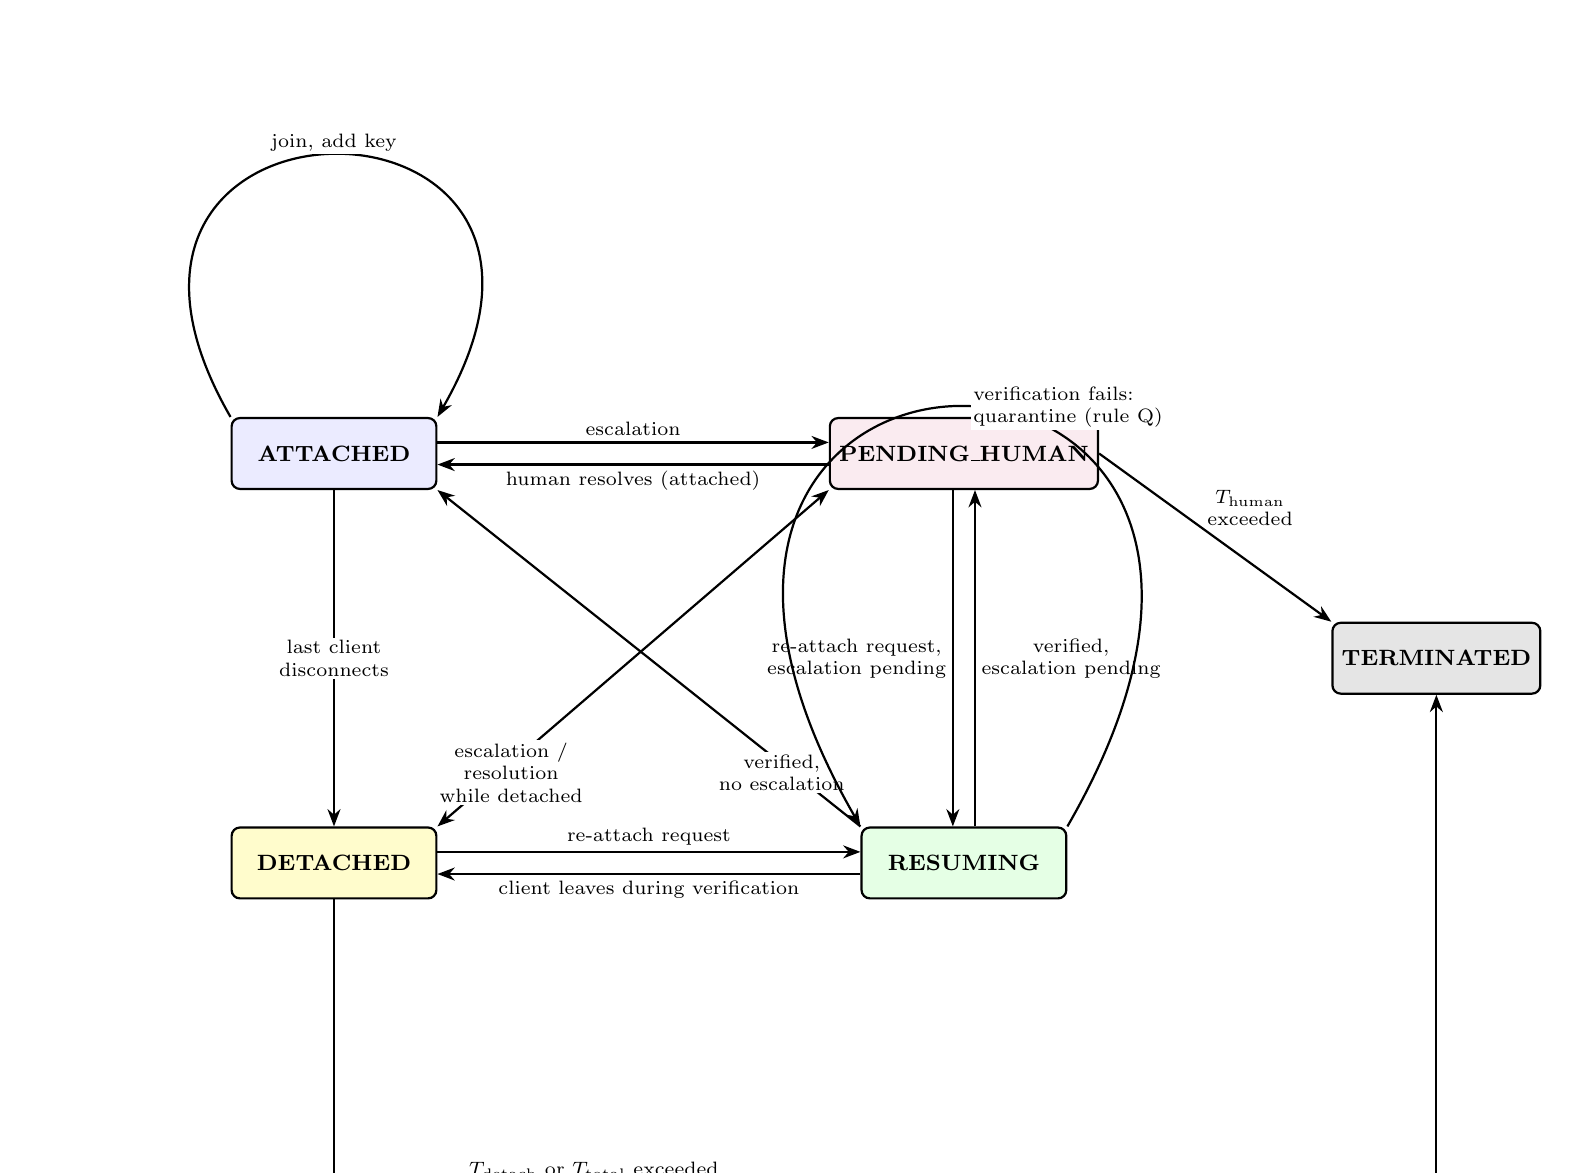
\begin{tikzpicture}[
  font=\footnotesize,
  st/.style={draw, rounded corners=3pt, thick, minimum width=2.6cm,
             minimum height=0.9cm, align=center, font=\footnotesize\bfseries},
  ed/.style={-{Stealth[length=2.2mm]}, thick},
  lb/.style={font=\scriptsize, fill=white, inner sep=1pt, align=center},
]
\node[st, fill=blue!8]   (att)  at (0,0)     {ATTACHED};
\node[st, fill=purple!8] (pend) at (8,0)     {PENDING\_HUMAN};
\node[st, fill=gray!20]  (term) at (14,-2.6) {TERMINATED};
\node[st, fill=yellow!20](det)  at (0,-5.2)  {DETACHED};
\node[st, fill=green!10] (res)  at (8,-5.2)  {RESUMING};

\draw[ed] (att) -- node[lb] {last client\\disconnects} (det);
\draw[ed] ([yshift=4pt]att.east) -- node[lb, above=1pt] {escalation} ([yshift=4pt]pend.west);
\draw[ed] ([yshift=-4pt]pend.west) -- node[lb, below=1pt] {human resolves (attached)} ([yshift=-4pt]att.east);
\draw[ed] ([yshift=4pt]det.east) -- node[lb, above=1pt] {re-attach request} ([yshift=4pt]res.west);
\draw[ed] ([yshift=-4pt]res.west) -- node[lb, below=1pt] {client leaves during verification} ([yshift=-4pt]det.east);
\draw[ed] (res.north west) -- node[lb, pos=0.16, xshift=-4pt] {verified,\\no escalation} (att.south east);
\draw[ed, {Stealth[length=2.2mm]}-{Stealth[length=2.2mm]}] (det.north east) -- node[lb, pos=0.16, xshift=4pt] {escalation /\\resolution\\while detached} (pend.south west);
\draw[ed] ([xshift=-4pt]pend.south) -- node[lb, left=1pt] {re-attach request,\\escalation pending} ([xshift=-4pt]res.north);
\draw[ed] ([xshift=4pt]res.north) -- node[lb, right=1pt] {verified,\\escalation pending} ([xshift=4pt]pend.south);
\draw[ed] (pend.east) -- node[lb, pos=0.45, above right] {$T_{\mathrm{human}}$\\exceeded} (term.north west);
\draw[ed] (det.south) -- ++(0,-3.6) -| (term.south);
\node[lb, anchor=south] at (3.3,-9.25) {$T_{\mathrm{detach}}$ or $T_{\mathrm{total}}$ exceeded};

\draw[ed] (att.north west) to[out=120, in=60, looseness=5]
  node[lb, above] {join, add key} (att.north east);
% Quarantine self-loop on RESUMING: drawn on the right side of RESUMING
% so it does not visually overlap the $T_{\mathrm{detach}}$ arrow that
% runs from DETACHED down and across to TERMINATED.
\draw[ed] (res.north east) to[out=60, in=120, looseness=8]
  node[lb, right=2pt, align=left] {verification fails:\\quarantine (rule~Q)} (res.north west);
\end{tikzpicture}
}
\caption{Derived view of named states of the Bridge Contract state machine.
Arrows are allowed transitions; each MUST emit a governance event before
mutating state (Invariant I7). A clean end or abort leads to TERMINATED from
every state, and a successful bridge restart leads to DETACHED; neither is
drawn. A failed verification or recovery quarantines the session and does not
terminate it. The normative model is the product machine of
Definition~\ref{def:sm}.}\label{fig:state-machine}
\end{figure}

In Table~\ref{tab:transitions}, $a$ and $h$ are placeholders for any
value of that dimension unless a value is stated; ``events'' lists the
events emitted, in order, before the cell changes (I7). The table lists
the transitions that change a cell, together with the join and re-attach
transitions that leave it as it is. Events that leave every cell
unchanged (tool-call events, \texttt{KEY\_REVOKED},
\texttt{OPERATOR\_ADD\_KEY}, narrowing, \texttt{AUTHORITY\_EXTENSION\_REJECTED})
are defined by the invariants (I2, I3, I10, I11-REVOKE, I13, I14), not by
a row of the table.

\begin{table}[htbp]
\centering
\caption{Allowed transitions over the product machine.}
\label{tab:transitions}
\footnotesize
\begin{tabularx}{\columnwidth}{l X X}
\toprule
\textbf{Transition} & \textbf{Precondition} & \textbf{Events} \\
\midrule
$(\textsc{Att},h) \to (\textsc{Det},h)$ & Transport disconnect of the
last connected client ($|C|=1$). & \texttt{DETACHMENT},
\texttt{RESUME\_PREPARED}. \\
$(\textsc{Att},h) \to (\textsc{Att},h)$ & Transport disconnect of one
client while others remain ($|C|\geq 2$). & \texttt{CLIENT\_LEFT}. \\
$(\textsc{Det},h) \to (\textsc{Det},h)$ & Idempotent disconnect (also of a
client that is not in $C$). & None. \\
$(\textsc{Att},h) \to (\textsc{Att},h)$ & Join: an authentic request
(I11) from a registered key, with a live unused nonce and a prefix of the
chain (I4, I9); $C := C \cup \{k\}$. & \texttt{CLIENT\_JOINED}; the
events after the acknowledged prefix are replayed to the joiner. \\
$(\textsc{Att},h) \to (\textsc{Att},h)$ & A registered client adds a
further key for the principal. & \texttt{CLIENT\_ADDED}. \\
$(a,\textsc{None}) \to (a,\textsc{Pend})$ & Agent escalates to a
human. & \texttt{HUMAN\_PENDING}; tool queue initialised. \\
$(a,\textsc{Pend}) \to (a,\textsc{Pend})$ & Second escalation while
one is pending: escalations coalesce. & \texttt{HUMAN\_PENDING}, recorded
for audit; the human dimension and $T_{\text{human}}$ (measured from the
first escalation) are unchanged. \\
$(a,\textsc{Pend}) \to (a,\textsc{None})$ & Human resolves. &
\texttt{HUMAN\_RESOLVED}, which ends every coalesced escalation at once.
The queue drains only once $a=\textsc{Att}$ (rule~D below). \\
$(\textsc{Det},h) \to (\textsc{Res},h)$ & Re-attach request that is
signed under a registered client key, uses a live unused nonce, and
names a prefix of the chain (I4, I9, I11). & \texttt{RESUME\_STARTED}. \\
$(a,h) \to (a,h)$, $a \neq \textsc{Res}$ & Re-attach or join request
with a bad signature or unknown key, a consumed, expired or unknown
nonce, a prefix the chain does not contain, or a reported 0-RTT replay
(I4, I8, I9, I11). & \texttt{RESUME\_REJECTED}; no state change. \\
$(\textsc{Att},h) \to (\textsc{Att},h)$ & Re-attach request, authentic
(I11) but made while the session is attached: join is the only way into an
attached session. & \texttt{RESUME\_REJECTED} (\texttt{already\_attached});
no state change, the nonce is spent. \\
$(\textsc{Res},h) \to (\textsc{Res},h)$ & Any further request while one is
being verified. & \texttt{RESUME\_REJECTED} (\texttt{resume\_in\_progress});
no state change. \\
$(\textsc{Res},h) \to (\textsc{Att},h)$ & Hash-chain verification
succeeds. & \texttt{RESUME\_VERIFIED}; then the queue drains (rule~D). \\
$(\textsc{Res},h) \to (\textsc{Det},h)$ & The re-attaching client
disconnects during verification. & \texttt{DETACHMENT}, \texttt{RESUME\_PREPARED}. \\
$(\textsc{Res},h) \to (\textsc{Res},h)$, quarantined & Hash-chain
verification fails (I5). & \texttt{RESUME\_FAILED}; no cell change; the
session is quarantined (rule~Q below). \\
$(\textsc{Det},h) \to \bot$ & $T_{\text{detach}}$ exceeded, or the time
spent detached over all episodes reached $T_{\text{total}}$. &
\texttt{DETACH\_TIMEOUT}, \texttt{TERMINATION}. \\
$(a,\textsc{Pend}) \to \bot$ & $T_{\text{human}}$ exceeded. &
\texttt{HUMAN\_TIMEOUT}, \texttt{TERMINATION}. \\
$(a,h) \to \bot$ & Clean session end or abort. & \texttt{TERMINATION}. \\
$(a,h) \to (\textsc{Det},h)$ & Bridge restart; recovery succeeds
(Section~\ref{sec:recovery}). & \texttt{BRIDGE\_RECOVERED},
\texttt{DETACHMENT}, \texttt{RESUME\_PREPARED}. \\
$(a,h) \to (a,h)$, quarantined & Bridge restart; recovery fails
(Section~\ref{sec:recovery}). & \texttt{RECOVERY\_FAILED}; no cell
change; the session is quarantined (rule~Q below). \\
\bottomrule
\end{tabularx}
\end{table}

\paragraph{Rule D (queue drain).} Queued tool calls drain, in arrival
order, whenever the session is in $(\textsc{Att},\textsc{None})$ with a
non-empty queue: that is, on \texttt{HUMAN\_RESOLVED} while attached, or
on \texttt{RESUME\_VERIFIED} when no escalation is outstanding. A human
who resolves while the client is detached or re-attaching leaves the
queue in place; it drains when the client is back. This is the
conservative reading of G1: the bridge cannot know that a queued call
is client-independent. Each call is re-validated at drain against the current scope, its own
lifetime and approval (I13) and its answer (I14); a call that fails is
not forwarded.

\paragraph{Forwarding acknowledgement.} A drained call passes through
stages that the log records separately: \emph{committed}
(\texttt{TOOL\_CALL\_DRAINED} is durable, I12), \emph{delivered} (the
runtime acknowledges receipt, \texttt{TOOL\_CALL\_DELIVERED}) and
\emph{completed} (the runtime reports the result,
\texttt{TOOL\_CALL\_COMPLETED}). The bridge forwards a call only after
its drain is committed, so a crash can leave a call committed but not
delivered. Such a call stays \emph{unacknowledged}: whenever the session is
in $(\textsc{Att},\textsc{None})$ and a bridge instance has not yet
forwarded an unacknowledged call, it forwards the call again with the
same idempotency key (I13), without a second drain event. A call that is
delivered is never forwarded again. Delivery is therefore at-least-once
with deduplication by the runtime; exactly-once execution is the runtime's
responsibility.

\paragraph{Calls outside an escalation (G1) --- conformance profiles.}
Rule D and I2 govern calls
that arrive while $h=\textsc{Pend}$. A call that arrives with
$h=\textsc{None}$ while $a\neq\textsc{Att}$ has no escalation to wait for,
and the contract gives the deployment a choice among the
\emph{conformance profiles} \texttt{refuse}, \texttt{queue} and
\texttt{forward}, fixed by configuration
and the same for every session of the deployment. The deployment
documents which profile it uses and, for the \texttt{forward} profile,
who may configure the forward allowlist (an operator role named in the
deployment documentation).
\begin{description}[leftmargin=2em]
\item[\texttt{refuse} (mandatory default).] The bridge refuses the call: it is not
queued, not forwarded and not recorded as a queued call, and the error
reaches the runtime. This profile is mandatory: every conformant
bridge MUST implement it, and it is the default if the deployment does
not name one. Every other statement in
this section assumes this profile unless it says otherwise.
\item[\texttt{queue} (optional).] The bridge queues the call
(\texttt{TOOL\_CALL\_QUEUED} with \texttt{held} set). It is held until a
human answers it (I14) and the session is in $(\textsc{Att},\textsc{None})$,
and is then forwarded under rule~D. A held call that is still unanswered
at drain is not rejected as unanswered; it waits and expires after
$T_{\text{call}}$ (I13). Held calls do not depend on an escalation, so
$T_{\text{approve}}$ does not apply to them.
\item[\texttt{forward} (optional).] The operator lists permissions that may run
without the client. A call whose permission is on that list and in the
current scope is recorded as queued, answered (source
\texttt{operator\_policy}) and drained in one committed batch, and
forwarded after the batch is durable (I12). Any other call is refused as
under \texttt{refuse}.
\end{description}
No profile changes I2: while $h=\textsc{Pend}$ every call is queued or
rejected under rule~D, whatever the profile. The \texttt{forward} profile
is the operator-defined exception to rule~D that a deployment opts into;
the bridge cannot tell on its own which calls are client-independent.

\paragraph{Rule Q (quarantine).} A session whose log cannot be vouched
for is \emph{quarantined}, not terminated. This applies when the hash
chain fails to verify after a re-attach was accepted
(\texttt{RESUME\_FAILED}), and when recovery after a restart finds the
chain broken
(\texttt{RECOVERY\_FAILED}); the cause is the storage or an attacker on it,
not the client, so ending the session would punish the wrong party and
destroy the evidence. The bridge MUST record the failure if it can still
append, MUST NOT emit \texttt{TERMINATION}, and MUST then refuse every
client operation on the session (attach, join, challenge, escalation,
tool call, authority change), run no timer on it and emit no further event
for it, except an operator's explicit termination (\texttt{TERMINATION}).
An operator's key addition is refused on a quarantined session
(\texttt{quarantined}), and no \texttt{CHECKPOINT} is appended to one. The session's
event log MUST be preserved read-only for forensic review: the bridge
MUST NOT append, truncate, or rewrite any record of a quarantined
session except the failure event that rule~Q itself permits and any
later \texttt{TERMINATION} the operator issues. The session
keeps the cell it had; quarantine is not a cell of the product machine,
and a restart does not lift it (the failure event is in the log; if it
could not be appended, recovery finds the broken chain again). Release
from quarantine is an operator action outside the contract; the only
action the contract permits on a quarantined session is operator
\texttt{TERMINATION}. Chain
verification follows authentication (I11), so a presenter without a
registered key cannot cause a quarantine. Quarantine is defence in depth
for a violated A1 (it freezes a session whose chain no longer verifies);
the guarantee of the safety argument rests on A1 and does not include it.

\subsection{Conformance Invariants}

\begin{invariant}[I1 --- Resume Preparedness]\label{inv:I1}
For every transition into a cell with $a=\textsc{Det}$ caused by a
disconnect (of the last connected client from $(\textsc{Att},h)$, or of
the re-attaching client from $(\textsc{Res},h)$), the bridge
MUST emit \texttt{DETACHMENT} followed by \texttt{RESUME\_PREPARED}
\emph{before} the cell changes.
\end{invariant}

\paragraph{Termination effects.}
On \texttt{TERMINATION}, the session enters $\bot$ (I6). The
following effects are normative:
\begin{itemize}[leftmargin=2em]
\item The tool-call queue is discarded; queued calls are not
forwarded. The runtime MUST be notified that the session is
terminated and SHOULD clean up any in-flight work.
\item In-flight tool calls (calls the bridge forwarded before
termination but whose \texttt{TOOL\_CALL\_COMPLETED} was not
emitted) are not tracked further; the runtime is responsible for
their disposition.
\item No timer runs on a terminated session; no further events are
emitted; no client operation is accepted (I6).
\item The event log is retained for audit (A1); the deployment
SHOULD apply its retention policy (Section~\ref{sec:limitations}).
\end{itemize}

\begin{invariant}[I2 --- Tool Call Suspension]\label{inv:I2}
While $h=\textsc{Pend}$, every tool call that the runtime submits to the
bridge for approval or forwarding MUST be either queued (with \texttt{TOOL\_CALL\_QUEUED} emitted) or rejected.
The bridge MUST NOT forward any tool call to the agent runtime for
execution while $h=\textsc{Pend}$. In-flight tool calls initiated
before \texttt{HUMAN\_PENDING} are not retracted; their completion is
audited as \texttt{TOOL\_CALL\_COMPLETED} (the separate completion event
of the forwarding acknowledgement, rule~D).
I2 covers what the runtime submits to the bridge; execution that the
bridge does not mediate is outside the contract (Section~\ref{sec:coverage}).
\end{invariant}

\begin{invariant}[I3 --- Authority Lock]\label{inv:I3}
In every cell, any attempt to widen \texttt{Authority-Scope} (any
proposed scope containing a permission that the current scope lacks)
MUST be rejected and MUST emit \texttt{AUTHORITY\_EXTENSION\_REJECTED};
the scope the bridge holds is unchanged. The scope of a session may only
narrow (I10). Widening requires a new attach with a freshly granted
scope, which is a new session. A tool call submitted while the session is
in $(\textsc{Att}, \textsc{None})$ with no human decision pending, whose
permission is not in the current scope, MUST be refused with the reason
\texttt{scope} and recorded as \texttt{TOOL\_CALL\_REJECTED} with
\texttt{direct} set; a call inside the scope is forwarded as before. I3 has two parts:
\begin{description}[leftmargin=2em]
\item[Enforced.] A change requested \emph{through the bridge} is refused
before it takes effect.
\item[Observed.] A change that the runtime announces \emph{itself} (for
example an Agent Client Protocol (ACP) agent switching its own mode; see
Section~\ref{sec:rw-agtp-thread} for the ACP disambiguation) has already happened when
the bridge learns of it. The bridge MUST emit
\texttt{AUTHORITY\_EXTENSION\_REJECTED} with source \texttt{observed}
and keep its record unchanged, and SHOULD instruct the runtime to revert
to the recorded scope. I3 does not claim that the bridge prevents a
runtime-initiated widening, only that it never records one as granted and
always reports it.
\end{description}
\end{invariant}

\begin{invariant}[I4 --- Prefix consistency]\label{inv:I4}
A re-attach or join request carries the pair $(\mathit{seq}, \mathit{hash})$ of
the last event the client acknowledged, taken from the event stream the
client observed, not from any artefact issued at detach. The bridge
MUST accept the request only if $\mathit{seq}$ does not exceed the
sequence number of the last committed event and $\mathit{hash}$ equals
the hash of the event with sequence number $\mathit{seq}$ in the bridge's
chain: that is, the client's history is a \emph{prefix} of the bridge's
chain. Any other pair (a different hash at that sequence, or a sequence
the chain has not reached) MUST be rejected with
\texttt{RESUME\_REJECTED} (reason \texttt{prefix\_mismatch}). Rejection
leaves the session in its current cell; it does not terminate the
session. On acceptance the bridge MUST deliver every committed event
after $\mathit{seq}$ to the client (the re-attaching or joining client),
including those that changed the
authority scope or the human dimension while the client was away; the
client reconciles its view from this replay.
\end{invariant}

\begin{invariant}[I5 --- Hash Chain Integrity]\label{inv:I5}
Every Governance Event MUST carry a \texttt{prev\_hash} field equal
to the SHA-256 of the canonical JSON of the immediately preceding
event in the same session. The genesis event's \texttt{prev\_hash}
MUST be the empty string.

I5 detects an insertion, deletion, rewrite or reordering of events in
the middle of the log. It does not detect the removal or rewrite of the
last events: a log cut back to an earlier event, or whose final event is
replaced, is again a valid chain. Detecting that requires the head
(sequence and hash) to be committed outside the log, as an
I-CHECKPOINT anchor does.
\end{invariant}

\begin{invariant}[I6 --- Terminality]\label{inv:I6}
The cell $\bot$ is terminal. Any subsequent operation that would
mutate state MUST raise an error. This covers every operation, including
attach, disconnect, join, add a client key, escalate, re-attach, submit
tool call, attempt authority extension, narrowing, human resolution, a
tool-call answer and the operator's key operations.
\end{invariant}

\begin{invariant}[I7 --- Event-before-Mutation]\label{inv:I7}
For every transition, the corresponding governance events MUST be
emitted and appended to the event log \emph{before} the cell is
changed. This ensures that the audit trail records the intent to
transition before the transition takes effect. Together with I12 this
ordering survives a bridge crash.
\end{invariant}

\subsection{Assumptions and Axioms}\label{sec:axioms}

The safety argument in Section~\ref{sec:safety-argument} rests on the
following assumptions, stated as axioms. A bridge implementation
operating in violation of any axiom is out of scope of this
specification.

\begin{description}[leftmargin=2em]
\item[A1 --- Reliable storage.] A record that has been committed under
I12 is not lost, reordered, or mutated by the storage medium or by the
bridge itself. (Mid-log tampering is detected by I5; truncation or
rewriting of the last events is not, without an external head.)
Rule~Q is defence in depth for a violated A1 and is not part of the
guarantee that rests on A1.
\item[A2 --- Monotonic sequence by construction.] The bridge's
sequence-number generator returns a strictly increasing value
on each call, including across restarts (it is recovered from the
log). Production of sequence numbers is monotonic by construction;
acceptance of client-claimed sequences is governed by I4.
\item[A3 --- SHA-256 collision resistance.] SHA-256 is collision
resistant under the assumed adversary. \texttt{prev\_hash} chaining
and the prefix check of I4 rely on this. The signature scheme of I11 is
assumed to be existentially unforgeable, and nonces are drawn from a
cryptographically secure source.
\item[A4 --- Trusted bridge.] The bridge is non-Byzantine: it does not
deliberately suppress governance events, forge events,
or lie about its state. (Byzantine bridge mitigations
are deployment-level, see \S\ref{sec:scope}.)
\item[A5 --- Serialised event emission per session.] Concurrent
event emission per session is serialised by the bridge's internal
locking. Concurrent sessions are independent. Because the dimensions of
the product machine are orthogonal, serialised events from different
dimensions (e.g., \texttt{DETACHMENT} and \texttt{HUMAN\_PENDING})
commute on the cell they reach.
\item[A6 --- Clocks.] While the bridge runs, timeouts use a monotonic
clock; wall-clock skew does not affect them. Across a restart, elapsed
time is taken from the timestamps of committed events, so a timeout may
fire late by at most the wall-clock error of the host. A host clock that
reads earlier than the last committed timestamp is treated as reading
that timestamp: no time is counted until the clock passes it, and
committed timestamps never decrease. Downtime counts toward
$T_{\text{human}}$, which is measured from the original
\texttt{HUMAN\_PENDING}, and toward $T_{\text{total}}$, but not toward
$T_{\text{detach}}$, which restarts at the recovered detachment
(Section~\ref{sec:recovery}). Fair scheduling
is assumed: the timeout check is eventually invoked (see
Appendix~\ref{app:formal-limitations}).
\item[A7 --- Key custody.] The private keys of registered clients are
not disclosed to the adversary, and the registry of client public keys
survives restarts (it is rebuilt from the log, I12). Compromise of a
client key is a deployment-level concern. The contract provides
operator-signed revocation (I11-REVOKE): a lost or compromised device
key can be revoked by the operator, after which it is no longer
accepted for re-attach or join. Soft revocation (\texttt{rotation})
keeps active connections; hard revocation (\texttt{compromise})
removes the key from the client set and detaches the session if that was
the last connected client. When all keys are revoked, the session enters
\texttt{key\_exhausted} (not rule~Q); the operator can add a new key
or terminate, and otherwise a detached session ends after the detachment
bound. Before revocation, a lost device stays authorised
until the session ends, which in the persistent profile can be
days; revocation is the operator's recovery path.
\end{description}

\subsection{Deployment requirements}
\label{sec:deployment-requirements}

The axioms above state what the contract assumes of the bridge and the
storage. A conformant deployment must additionally provide what
Table~\ref{tab:deployment-requirements} lists; the table makes explicit
what the baseline MUSTs leave to the operator.

\begin{table}[htbp]
\centering
\caption{Assumptions and deployment requirements.}
\label{tab:deployment-requirements}
\footnotesize
\begin{tabularx}{\columnwidth}{l X}
\toprule
\textbf{Requirement} & \textbf{What the deployment must provide} \\
\midrule
Append-only storage &
A storage medium that, once a record is committed under I12, does not
lose, reorder, or mutate it (A1). Mid-log tampering is detected by I5;
truncation of the tail is detected only against a head held outside the
log, and, if required, by I-SIGN-EVENT and I-CHECKPOINT. \\
Trusted bridge &
A non-Byzantine bridge (A4): one that does not deliberately suppress
governance events, forge events, or lie about its state. Byzantine-bridge
mitigations are deployment-level (external transparency logs). \\
Client-key custody &
The principal holds the private keys of every registered client key
(A7); the contract provides operator-signed revocation (I11-REVOKE)
for lost or compromised keys. Soft revocation (\texttt{rotation})
keeps active connections; hard (\texttt{compromise}) removes the key
from the client set and detaches the session if it was the last
connected client. When
all keys are revoked, the session enters \texttt{key\_exhausted};
the operator adds a new key or terminates, and otherwise a detached
session ends after the detachment bound. \\
Human-resolution and answer channel &
An authenticated channel for \texttt{HUMAN\_RESOLVED},
\texttt{TOOL\_CALL\_ANSWERED} and a clean end of session. The deployment
documents who may emit them and under which key. The contract does not
specify the channel; the bridge trusts whatever the deployment feeds it. \\
Runtime idempotency contract &
The runtime deduplicates forwarded calls by idempotency key. The key
scope is the session. The deployment states a retention bound for
spent keys. A second submission of the same key with different content
is rejected: this is a MUST while the first call is queued (I13,
reason \texttt{duplicate\_key}); for a key already spent, the same
rejection is a SHOULD that holds within the deployment's retention
bound, and beyond that bound the contract states no requirement.
\texttt{DELIVERED}
means receipt, not execution; exactly-once external effects are not
guaranteed. \\
Runtime routes execution and authority through the bridge &
Where the deployment wants the bridge to enforce (rather than observe)
authority, the runtime routes every authority change and every
tool-call submission through the bridge. Execution the bridge does not
mediate is outside the contract (Section~\ref{sec:coverage}). \\
Log access authorisation and retention &
The deployment documents who may read the event log and the replay, and
the bridge enforces a retention bound after which the log is archived or
destroyed (Section~\ref{sec:limitations}). \\
\bottomrule
\end{tabularx}
\end{table}

\subsection{Lemmas}\label{sec:lemmas}

The following lemmas are immediate consequences of the invariants and
axioms. Their proofs are short and are provided for completeness.

\begin{lemma}[Audit ordering]\label{lem:atomicity}
I5 $+$ I7 $+$ I12 $\Rightarrow$ no externally observable change of cell
exists without its governing events already committed in the log, and
the log alone determines the cell that recovery rebuilds.
\end{lemma}

\begin{proof}[Sketch.]
I7 requires the events to be appended before the cell changes, and I12
requires the append to be durable before the change and before any
acknowledgement to the client. I5 links each event to its predecessor.
Therefore any cell visible to a client, or recoverable after a crash,
is preceded by a verifiable committed event. A crash between the append
and the change leaves the log ahead of the cell; recovery
(Section~\ref{sec:recovery}) resolves this in favour of the log. The
lemma asserts ordering, not atomicity: it does not claim that append and
change occur indivisibly. \qedhere
\end{proof}

\begin{lemma}[No authority drift]\label{lem:no-drift}
I3 $+$ I10 $\Rightarrow$ in every cell, at every point of an execution,
the authority scope that the bridge holds for a session is a subset of
its scope at attach. (The runtime's effective authority equals it only
for changes requested through the bridge; see I3, observed.)
\end{lemma}

\begin{proof}[Sketch.]
The scope is changed only by an accepted narrowing (I10); every
widening attempt is rejected without changing it (I3). By induction
over the transitions, the scope after each step is a subset of the scope
before it, hence of the scope at attach. \qedhere
\end{proof}

\begin{lemma}[Resume recoverability]\label{lem:recover}
I1 $+$ I4 $+$ I5 $+$ I11 $\Rightarrow$ on an authenticated re-attach,
the client is brought to the bridge's current state by a verifiable
replay of the events it has not seen.
\end{lemma}

\begin{proof}[Sketch.]
I1 forces \texttt{RESUME\_PREPARED} to be emitted and stored before the
cell changes to $a=\textsc{Det}$, so the resume point is recorded
durably. I11 ensures the presenter holds a registered client key and
answers a fresh nonce, so the request is neither forged nor replayed. I4
ensures that the $(\mathit{seq}, \mathit{hash})$ the client presents lies
on the bridge's chain, and I5 ensures that every event after it carries
the \texttt{prev\_hash} of its predecessor, so the client can verify the
replay against the hash it already holds. Hence the client's resulting
view is a causally consistent extension of what it had acknowledged.
\qedhere
\end{proof}

\begin{lemma}[Terminality]\label{lem:terminality}
I6 $\Rightarrow$ after $\bot$, no further state mutation is
possible for the session.
\end{lemma}

\begin{proof}[Sketch.]
The lemma restates I6: I6 forbids every state-mutating operation on a
session in $\bot$, and $\bot$ has no outgoing transition in
Table~\ref{tab:transitions} ($F=\{\bot\}$). \qedhere
\end{proof}

\subsection{Liveness properties}\label{sec:liveness}

The Bridge Contract's liveness properties depend on the timeouts
defined in \S\ref{sec:timeouts}. Without timeouts the contract
satisfies safety but not liveness: a session could remain in a cell
with $a=\textsc{Det}$ or $h=\textsc{Pend}$ indefinitely. The following
liveness properties hold \emph{conditionally on the bridge's timer
mechanism being scheduled fairly} (Axiom A6; see
Appendix~\ref{app:formal-limitations} for the fairness limitation in the
formal model). Without a fairness assumption on the scheduler, L1 and L2
do not hold: a scheduler that indefinitely postpones the timeout check
would leave the session in such a cell forever, which does not violate
any safety invariant but violates liveness.

\begin{description}[leftmargin=2em]
\item[L1.] \emph{(conditional on fair scheduling, A6)} For every
session that enters a cell with $a=\textsc{Det}$, either the client
re-attaches successfully (through $a=\textsc{Res}$ to
$a=\textsc{Att}$), or the session reaches $\bot$ within
$T_{\text{detach}}$ of that detachment, or it is quarantined (the exception
discussed after L2). A \texttt{key\_exhausted} session is no exception: its
timers keep running, so unless the operator adds a key it reaches $\bot$
within $T_{\text{detach}}$ as well. Over the whole session, the time
spent in cells with $a=\textsc{Det}$, summed over all detachments and
including time during which the bridge was down, never exceeds
$T_{\text{total}}$: once it has used up $T_{\text{total}}$, a session in
$a=\textsc{Det}$ reaches $\bot$ even if no single detachment has lasted
$T_{\text{detach}}$ (the model checks that it then leaves $a=\textsc{Det}$,
by a re-attach in progress, or ends, or is quarantined; \texttt{CapEnds}).
A re-attach does not depend on any artefact issued
at detach (I4, I11), so no secondary expiry can terminate the session
earlier.
\item[L2.] \emph{(conditional on fair scheduling, A6)} For every session
that enters a cell with $h=\textsc{Pend}$, either the human resolves
(the session moves to $h=\textsc{None}$) or the session reaches
$\bot$ within $T_{\text{human}}$ of the first escalation, or earlier if
the detach timeout fires first, or the session is quarantined. The
human timer of a \texttt{key\_exhausted} session keeps running. While $a=\textsc{Det}$ the detach
timer runs (it is stopped in $a=\textsc{Res}$), so a human wait never outlasts the detachment the deployment
tolerates; while the client is attached the wait may be longer than
$T_{\text{detach}}$ if $T_{\text{human}}$ is.
\end{description}

L1 and L2 together imply that no active session that is not quarantined
remains in a transient cell indefinitely (under fair scheduling), with one
reservation about a \texttt{key\_exhausted} session: while a client is
still connected on a softly revoked key the cell is $a=\textsc{Att}$ and no
detach timer runs, until the transport is lost or the operator acts (the
hazard of rotating the only key is described under Key exhaustion).
$\bot$ is the only
cell in which a session may persist without bound, apart from
$(\textsc{Att},\textsc{None})$, which has no timer and is stable by design,
and from a quarantined session, which is frozen by rule~Q until an operator
acts. A re-attach
cannot hold the session in $a=\textsc{Res}$ without bound, because a
client disconnect during verification returns it to $a=\textsc{Det}$ and
verification itself is a finite computation over the log. A re-attach that
is started and abandoned repeatedly is a limit of this bound: time in
$a=\textsc{Res}$ and $a=\textsc{Att}$ is not counted by $T_{\text{total}}$,
so $T_{\text{total}}$ does not bound such a cycle. A revocation of the only key while it is being
verified, soft or hard, abandons the verification and the session returns
to $a=\textsc{Det}$, where the detach timer runs.

\subsection{Timeouts}\label{sec:timeouts}

The state machine depends on the timers of Table~\ref{tab:timers}.
$T_{\text{human}}$, $T_{\text{call}}$ and $T_{\text{total}}$ default from
$T_{\text{detach}}$; $T_{\text{approve}}$ and $T_{\text{nonce}}$ do not
(Table~\ref{tab:timer-profiles}). The
applicability of $T_{\text{detach}}$ and $T_{\text{human}}$ to each cell
is:

\begin{center}
\small
\begin{tabular}{l l l}
\toprule
\textbf{Cell} & $T_{\text{detach}}$ & $T_{\text{human}}$ \\
\midrule
$(\textsc{Att},\textsc{None})$ & --- & --- \\
$(\textsc{Att},\textsc{Pend})$ & --- & running \\
$(\textsc{Det},\textsc{None})$ & running & --- \\
$(\textsc{Det},\textsc{Pend})$ & running & running \\
$(\textsc{Res},\textsc{None})$ & stopped & --- \\
$(\textsc{Res},\textsc{Pend})$ & stopped & running \\
\bottomrule
\end{tabular}
\end{center}

\begin{table}[htbp]
\centering
\caption{The timers: start event, clock source, pause/reset
behaviour, survival across a bridge restart, expiry event and
interactions. Defaults and bounds are listed in
Table~\ref{tab:timer-profiles}.}
\label{tab:timers}
\scriptsize
\begin{tabularx}{\columnwidth}{l X X X X X}
\toprule
\textbf{Timer} & \textbf{Starts on} & \textbf{Clock} & \textbf{Pause / reset} & \textbf{Survives restart?} & \textbf{Expiry event} \\
\midrule
$T_{\text{detach}}$ &
The \texttt{DETACHMENT} that begins a detachment; not restarted by later events while detached. &
Monotonic while running; across a restart, elapsed time is taken from committed event timestamps (A6). &
Stopped while $a=\textsc{Res}$; a return from $a=\textsc{Res}$ to $a=\textsc{Det}$ is a new \texttt{DETACHMENT} and starts a fresh interval ($T_{\text{total}}$ keeps counting the time spent detached, so that time is bounded over the cycle; a re-attach started and abandoned repeatedly is not bounded by $T_{\text{total}}$, which does not count time in $a=\textsc{Res}$); reset to a fresh interval by a bridge restart while detached (recovery rule~2). &
The interval is reset (the restart begins a new detachment). &
\texttt{DETACH\_TIMEOUT}, \texttt{TERMINATION}. \\
$T_{\text{total}}$ &
The first \texttt{DETACHMENT} of the session; summed over every away interval. &
Computed from committed event timestamps; never held as an in-memory timer. &
Never reset; time in $a=\textsc{Res}$ and $a=\textsc{Att}$ is not counted; bridge downtime while detached is counted. &
Yes --- downtime is part of the away interval. &
\texttt{DETACH\_TIMEOUT}, \texttt{TERMINATION}. \\
$T_{\text{human}}$ &
The first \texttt{HUMAN\_PENDING} of the current escalation; a second escalation while one is pending does not restart it. &
Monotonic while running; across a restart, elapsed time is taken from the original \texttt{HUMAN\_PENDING} (A6). &
Running while $h=\textsc{Pend}$; stopped when $h=\textsc{None}$; bridge downtime while $h=\textsc{Pend}$ counts toward it. &
Yes --- measured from the original \texttt{HUMAN\_PENDING}; an elapsed timeout is applied after recovery. &
\texttt{HUMAN\_TIMEOUT}, then \texttt{TERMINATION}. \\
$T_{\text{call}}$ &
The \texttt{TOOL\_CALL\_QUEUED} event of the call. &
Monotonic. &
Not paused; expires even if the queue is held under the \texttt{queue} profile. The call is removed on expiry. &
Yes (queued in the log); a call whose $T_{\text{call}}$ elapsed during downtime is expired at recovery. &
\texttt{TOOL\_CALL\_EXPIRED}; the call is not forwarded. \\
$T_{\text{approve}}$ &
The \texttt{HUMAN\_RESOLVED} event of the escalation. &
Monotonic. &
Not paused; runs even while the client is away. An approval that lapses is void at the next drain. &
Yes (queued in the log). &
\texttt{TOOL\_CALL\_EXPIRED} on every call of the lapsed escalation at the next drain; the expiry is recorded per call when the approval is given, so a later approval does not revive it. \\
$T_{\text{nonce}}$ &
The bridge issues a challenge and returns a nonce. &
Monotonic; the bridge's own clock. &
Not paused; the nonce is volatile and is void after a restart. &
No --- outstanding nonces are void; the client asks for a fresh challenge. &
The nonce is rejected on next use with \texttt{RESUME\_REJECTED} (reason \texttt{nonce\_expired}). \\
\bottomrule
\end{tabularx}
\end{table}

\paragraph{Derivation of the timers.} The timers are not independent:
\[
T_{\text{call}} \;\leq\; T_{\text{human}}
\qquad\text{and}\qquad
T_{\text{detach}} \;\leq\; T_{\text{total}}
\qquad (\text{MUST}),
\]
and $T_{\text{human}}$ defaults to $T_{\text{detach}}$,
$T_{\text{call}}$ to $T_{\text{human}}$ and $T_{\text{total}}$ to four
times $T_{\text{detach}}$. $T_{\text{call}} \leq T_{\text{human}}$ is a configuration simplification:
a call may not outlive the longest wait the session tolerates (under the
\texttt{queue} profile a held call has no escalation, but is bounded the
same way). The cap is useless if it is below a single detachment.
$T_{\text{human}} \leq T_{\text{detach}}$ is a recommendation that the
profiles follow, not a configuration bound: it constrains a session only
where the client is away, and there the detach timer enforces it without
help, because a detached session ends at $T_{\text{detach}}$ whatever the
human timer says. With the client attached, an escalation may wait longer
than $T_{\text{detach}}$ if the deployment sets $T_{\text{human}}$ so. When
the client then detaches, the wait is bounded by the time that remains of
$T_{\text{human}}$ and by $T_{\text{detach}}$ from the detachment,
whichever ends first. Independent defaults (for example 24~h and 1~h) that
did not follow from $T_{\text{detach}}$ would end work that a mobile owner
expects to survive a long detach. A deployment chooses one
\emph{profile}:

\begin{table}[htbp]
\centering
\caption{Timer profiles. Defaults are informative; operators MAY set
the timers to any non-negative values that satisfy the bounds above (the
value 0 is degenerate: a nonce expires on issue, a detachment ends at
once).}
\label{tab:timer-profiles}
\footnotesize
\begin{tabular}{l r r r r r r}
\toprule
\textbf{Profile} & \makebox[1.4cm]{$T_{\text{detach}}$} & \makebox[1.4cm]{$T_{\text{human}}$} &
\makebox[1.2cm]{$T_{\text{call}}$} & \makebox[1.4cm]{$T_{\text{total}}$} & \makebox[1.3cm]{$T_{\text{approve}}$} &
\makebox[1.1cm]{$T_{\text{nonce}}$} \\
\midrule
interactive-short (default) & 30 min & 30 min & 30 min & 2 h & 15 min & 60 s \\
persistent & 7 days & 7 days & 7 days & 28 days & 15 min & 60 s \\
\bottomrule
\end{tabular}
\end{table}

\noindent $T_{\text{approve}}$ (I13) is a freshness bound on an approval,
not a liveness bound on the session, and is deliberately independent: in
the persistent profile an approval given while the client is away still
expires after 15 minutes and the call is rejected at drain, so the agent
must ask again. A deployment that wants approvals to outlive a detachment
raises $T_{\text{approve}}$ and accepts the weaker freshness.

\paragraph{Interaction.} In $(\textsc{Det},\textsc{Pend})$ both timers
run and whichever fires first terminates the session; the cumulative cap
$T_{\text{total}}$ runs in the same cells and ends the session if it is
reached first. Because a detached session ends at $T_{\text{detach}}$
regardless, holding it open for a longer $T_{\text{human}}$ would serve
no purpose. A deployment that must wait on a human for longer while the
client is away MUST raise $T_{\text{detach}}$ (and $T_{\text{total}}$)
accordingly.

\paragraph{Conflict resolution (both timeouts fire simultaneously).}
If both timeouts expire in the same tick in
$(\textsc{Det},\textsc{Pend})$, the bridge MUST:
\begin{enumerate}[leftmargin=2em]
\item Emit \texttt{HUMAN\_TIMEOUT} (the human-side timeout event);
\item Emit \texttt{DETACH\_TIMEOUT} (the detach-side timeout event,
to preserve audit completeness --- suppressing it would lose
information about which timeouts fired, contradicting the
event-completeness rationale of Table~\ref{tab:event-completeness});
\item Emit \texttt{TERMINATION} with reason field
\texttt{human\_timeout+detach\_timeout (simultaneous)};
\item Transition to $\bot$.
\end{enumerate}
The order is fixed: \texttt{HUMAN\_TIMEOUT}, then
\texttt{DETACH\_TIMEOUT}, then \texttt{TERMINATION}, so that two logs of the
same run are equal. The choice of \texttt{human\_timeout} as the leading
reason-token in (3) follows a default priority rule, not an
alphabetical one: the human escalation is the semantically more salient event for
audit consumers. The bridge
SHOULD apply this default consistently across all simultaneous-timeout
cases; operators MAY override the default priority via configuration
(e.g., to prefer \texttt{detach\_timeout} in deployments where
detach is the more salient signal). An override changes only the leading
token of the reason in (3), never the order of the events. An override is a
deployment configuration, not a contract violation.

\paragraph{Edge cases (normative).}
\begin{enumerate}[leftmargin=2em]
\item \emph{Timer expiry in the same tick as an incoming request.}
If a timer expires in the same tick as an incoming request that would
move the session out of the timed cell (for example, $T_{\text{detach}}$
expiring in the same tick as a re-attach request that names a valid
prefix), the bridge MUST process the request first. If the request
succeeds (e.g., \texttt{RESUME\_STARTED}), the timer is no longer
applicable to the new cell and is not fired. If the request fails
(e.g., \texttt{RESUME\_REJECTED}), the timer fires in the same tick
and the session transitions accordingly. The reference bridges follow the
rule: a timer that expires in the tick of a re-attach or a join waits for the
request, and one that expired in an earlier tick has ended the session, so
the request is refused uniformly. The one exception is $T_{\text{human}}$: it
wins over a resolve that arrives in its own tick (a resolve is the only request
that moves a session out of the pending-approval cell; every other request
leaves the session in that cell, so the rule above does not apply to it). The bridge ends the session
with \texttt{HUMAN\_TIMEOUT} and \texttt{TERMINATION}, refuses the resolve and
answers it \texttt{terminated}.
\item \emph{The same idempotency key arriving with different content.}
A second tool call submitted with an idempotency key that is already
queued MUST NOT be queued, regardless of whether the content matches
or differs from the first submission; the caller is answered with the
reason \texttt{duplicate\_key}. The first submission's content
and hash are retained; the second is discarded and commits no event, so
the queued record is returned and the log does not record the second
submission (limitations register).
\end{enumerate}

\paragraph{Configuration.} Default values are informative.
Operators MAY set the timers to any values $\geq 0$ that satisfy the
bounds above. A timeout of $0$ means ``immediate termination on entry to the cell''; this is
useful for testing and for deployments that prefer fail-fast.
With $T_{\text{detach}} = 0$: on entry to a cell with $a=\textsc{Det}$,
the bridge MUST still emit \texttt{DETACHMENT} +
\texttt{RESUME\_PREPARED} (per I1) before transitioning to $\bot$ with
\texttt{DETACH\_TIMEOUT} + \texttt{TERMINATION}.

\subsection{Bridge restart and recovery}\label{sec:recovery}

When the bridge process restarts with live sessions, it MUST recover
each session from its durable event log (I12) before accepting any
client message for it. The rules are:

\begin{enumerate}[leftmargin=2em]
\item \textbf{Replay.} Read the committed log from genesis (or from the
latest verified checkpoint, I-CHECKPOINT), verify the hash chain (I5),
and rebuild the cell, the scope and \texttt{scope\_version}, the
registry of client keys, the tool queue, the idempotency keys, and the
timer anchors. A trailing record
that is not fully durable is discarded; by I12 it has no externally
visible effect.
\item \textbf{Transports are gone.} Every client transport was lost with
the process, so every recovered active session has an empty client set
and $a=\textsc{Det}$; the registered keys $K$ are rebuilt from the log,
with the scheme tag and public key each event records, and the key registry
in storage is repaired from them: the log is the source of truth, so a key
missing from the registry is written back, an entry the log does not record
(a crash between the registry write and the event commit leaves one) is
dropped, and an entry whose scheme or public key differs from the log is
replaced. \texttt{BRIDGE\_RECOVERED} names the key ids repaired.
The bridge MUST emit \texttt{BRIDGE\_RECOVERED}, then \texttt{DETACHMENT}
(reason \texttt{bridge\_restart}) and \texttt{RESUME\_PREPARED} (the
resume record of the new detachment), before the cell changes.
$T_{\text{detach}}$ restarts at the new \texttt{DETACHMENT}; the
cumulative cap $T_{\text{total}}$ does not (a restart while detached
continues the away interval, downtime included). Challenge
nonces are volatile and are void after a restart: a client that holds
one simply requests another (I11).
\item \textbf{Elapsed timeouts.} $T_{\text{human}}$ is measured from the
original \texttt{HUMAN\_PENDING} (A6). If it has already elapsed, the
bridge MUST terminate the session after recovery with
\texttt{HUMAN\_TIMEOUT} and \texttt{TERMINATION}. Likewise, if the
cumulative cap $T_{\text{total}}$ has already been reached (downtime
included), the reference bridge terminates the session after recovery with
\texttt{DETACH\_TIMEOUT} and \texttt{TERMINATION}; $T_{\text{detach}}$
itself has just restarted and cannot have elapsed. The expiry of an
approval, $T_{\text{approve}}$, is recorded as \texttt{valid\_until} in
\texttt{HUMAN\_RESOLVED}; recovery reads it back from the log, so an approval
that had lapsed before the restart stays lapsed.
\item \textbf{Recovery failure.} If the chain does not verify, the
bridge MUST NOT resume the session and leaves the key registry as it is.
The bridge quarantines the session (rule~Q): it
emits \texttt{RECOVERY\_FAILED} if it can still append, emits no
\texttt{TERMINATION}, and leaves the session to an operator.
A log that cannot be replayed at all (no \texttt{ATTACHED} event first, or
one without the fields the session is built from) quarantines its own
session in memory, appends nothing to it, and does not stop the recovery
of the other sessions. A chain
failure found during a re-attach is handled the same way, because the
cause is the same and is not attributable to the client.
\item \textbf{In-flight tool calls.} A call whose drain was committed
but whose delivery the runtime did not acknowledge before the crash
(\texttt{TOOL\_CALL\_DELIVERED}) is forwarded again, with the same
idempotency key (I13), when the session is back in
$(\textsc{Att},\textsc{None})$ (rule~D); it is not drained twice. A call
that was queued but not drained is subject to the usual drain checks. The
runtime deduplicates by key. Delivery is therefore at-least-once with
deduplication, never silently lost, and a call that was committed as
drained is never dropped silently either.
\end{enumerate}

Bridge availability (replication, failover to another host) is a
deployment concern beyond this rule: the rules above hold for any bridge
instance that has the durable log and the registered client keys.

\subsection{Additional invariants}\label{sec:additional-invariants}

The following invariants are conditioned on deployment-specific
concerns or strengthen the core set $\{I_1, \ldots, I_7\}$. They are
stated here to make normative requirements that would otherwise live
in \S\ref{sec:limitations} live instead in the specification.

\subsubsection{Event signing (Invariants I-SIGN-EVENT and I-SIGN-JWKS)}\label{sec:invariants-signing}

\begin{invariant}[I-SIGN-EVENT --- Event signing in GEC-less deployments (SHOULD)]
\label{inv:isign-sign}
In a GEC-less deployment (Definition~\ref{def:gecless}), the bridge
SHOULD sign each emitted event with an operator key whose JWKS
endpoint is published through an out-of-band channel bound to the
operator's deployment identity (per GAR \S 6.1).
In a GEC-present deployment, the bridge forwards unsigned events to
the GEC for signing; I-SIGN-EVENT is vacuous.
\end{invariant}

\begin{invariant}[I-SIGN-JWKS --- JWKS endpoint source restriction (MUST)]
\label{inv:isign-jwks}
The bridge MUST NOT accept a JWKS endpoint learned from
session-supplied metadata. The JWKS endpoint used by the bridge for
event signing (or for forwarding to the GEC) MUST be configured via
an out-of-band channel bound to the operator's deployment identity.
A JWKS endpoint learned from the client or from session-supplied
metadata is not a trust anchor.
\end{invariant}

I-SIGN-EVENT is SHOULD (not MUST) because event signing requires
operator key management infrastructure that may not be available in
testing or small deployments. Operators who omit signing accept
that downstream consumers cannot verify event provenance without an
out-of-band trust channel. I-SIGN-JWKS is MUST because accepting
session-supplied JWKS endpoints would allow the client (or an
adversary) to substitute a different signing key, breaking the
trust model; this is not optional regardless of deployment size.

\subsubsection{QUIC 0-RTT replay (Invariant I8)}\label{sec:invariants-quic}

\begin{invariant}[I8 --- QUIC 0-RTT replay rejection]\label{inv:I8}
The bridge MUST NOT accept a client re-attach whose underlying
transport is a replayed QUIC 0-RTT session. Replay detection is
governed by AGTP-SESSION \S 10.5, which forbids establishing a session in
0-RTT data, and by the replay-safety profile of AGTP-BINDINGS \S 4.6, which
restricts early data to safe idempotent methods \cite{I-D.hood-agtp-bindings};
the bridge defers to the transport layer for replay identification and rejects the re-attach (with
\texttt{RESUME\_REJECTED}) if the transport reports a replay.
\end{invariant}

I8 is conditioned on the transport layer's replay detection. In
deployments that do not use QUIC 0-RTT, I8 is vacuous. In deployments
that do, the bridge's responsibility is to \emph{honour} the
transport's replay verdict, not to perform replay detection itself.

\subsubsection{Challenge nonce lifetime (Invariant I9)}
\label{sec:invariants-ttl}

\begin{invariant}[I9 --- Challenge nonce lifetime]\label{inv:I9}
A challenge nonce (I11) is valid for $T_{\text{nonce}}$ after the bridge
issued it, measured on the bridge's monotonic clock (A6). A re-attach
that presents a nonce older than $T_{\text{nonce}}$ MUST be rejected
with \texttt{RESUME\_REJECTED} (reason \texttt{nonce\_expired}). The
rejection does not change the cell and does not terminate the session:
only a timeout ($T_{\text{detach}}$, $T_{\text{total}}$ or, while an
escalation is pending, $T_{\text{human}}$) ends a detached session. \emph{Default:}
$T_{\text{nonce}} = 60$~seconds. \emph{Configurable:} yes,
per-deployment.
\end{invariant}

A design that bounds the lifetime of a resume token issued at detach,
and terminates the session when it expires, cannot serve a client that vanished abruptly: the token is minted when
the client is already gone and has nowhere to be delivered. The
challenge is instead minted when the client asks for it, so its
lifetime can be short without ever stranding the client; I9 bounds the
window in which a captured nonce and signature could be replayed, and
nothing else.

\subsubsection{Authority scope versioning (Invariant I10)}
\label{sec:invariants-scope-version}

\begin{invariant}[I10 --- Authority scope versioning]\label{inv:I10}
The session's authority scope carries a monotonically increasing
\texttt{scope\_version} counter, incremented on each successful
narrowing (i.e., each \texttt{AUTHORITY\_NARROWED} event), in every
cell. The counter starts at 0 at attach. Each
\texttt{AUTHORITY\_NARROWED} event MUST include
\texttt{new\_version} = \texttt{previous\_version} + 1 and a scope that
is a strict subset of the current scope. A duplicate or out-of-order
narrowing, or one whose proposed scope equals the current scope, MUST be
rejected with \texttt{AUTHORITY\_NARROWING\_REJECTED}; a proposal that
widens the scope is governed by I3 and is rejected with
\texttt{AUTHORITY\_EXTENSION\_REJECTED}. A proposal that is not a strict
subset of the current scope is therefore rejected: if it contains any
permission the current scope lacks, including a partial overlap that also
drops permissions, it is an extension and is rejected as above. A scope change that happened
while the client was away is not a reason to refuse its re-attach: it is
part of the replay that I4 requires, and the client reconciles to the
new scope.
\end{invariant}

I10 gives auditors a monotonic history of authority scope changes per
session. Regulators can trace the scope trajectory from attach
(version 0) through any narrowings (versions 1, 2, \ldots) to the
current state. With I3 it makes the authority of a session
non-increasing for its entire life.

\subsubsection{Challenge-response resume (Invariant I11)}
\label{sec:invariants-token-auth}

\begin{invariant}[I11 --- Authenticated single-use challenge]\label{inv:I11}
\begin{enumerate}[leftmargin=2em,label=(\alph*)]
\item \emph{Key binding.} The client registers a public key at attach;
the key is recorded in the genesis \texttt{ATTACHED} event and bound to
\texttt{Owner-ID}.
\item \emph{Challenge.} To re-attach, the client first requests a
challenge, naming the key identifier it will sign with. The bridge
returns a fresh nonce of at least 128 bits from a
cryptographically secure source, bound to the session and to that key
identifier, valid for $T_{\text{nonce}}$ (I9) and usable once. The record of
the nonce holds the key identifier and whether the key was a registered,
unrevoked key of the session when the nonce was issued. The answer to a
challenge is the same for every key identifier, registered or not: a nonce of
the same form and lifetime, counted against the same limit (f); no answer to
a challenge depends on the registry. A nonce issued for a key that was not
registered at issue never verifies, however the registry changes later, and a
nonce presented with another key identifier than the one it was issued for
does not verify either; both are answered as a request whose signature does
not verify (\texttt{bad\_signature}), recorded as \texttt{nonce\_binding} and
not spent. Issuing a challenge is not a
governance event and changes no state. The bridge SHOULD return a uniform rejection
to unauthenticated callers (e.g., for an unknown session ID) so
that the \texttt{challenge} op does not confirm session existence
or lifecycle state. Nonces are not durable (Section~\ref{sec:recovery}).
\item \emph{Proof of possession.} The re-attach request carries
$(\mathit{nonce}, \mathit{seq}, \mathit{hash})$ and a signature, under
a registered client key, over the tuple of Appendix~\ref{app:wire-format}
(signature scope), which binds the operation (re-attach or join), the
session, the key id, the nonce and the prefix. The request is authentic
iff the signature verifies for the operation received. A request that
names a key id the session does not register is answered as one whose
signature does not verify (\texttt{bad\_signature}), so the answer does not
list the registered key ids; the log records \texttt{unknown\_key}. A
registration of a further key (\texttt{add\_client}) is verified in the same
order: the signature first, and the lifecycle of the session (unknown,
terminated, quarantined, key-exhausted) is named only to a caller whose
signature verified; any other caller is answered \texttt{bad\_signature}.
\item \emph{Single use.} A nonce is consumed by the first authentic
request that presents it, whether that request is then accepted or
rejected for a later reason; a consumed nonce is never accepted again.
A request that is not authentic does not consume the nonce. A request
refused with \texttt{resume\_in\_progress}, \texttt{already\_attached} (a
re-attach on an attached session) or \texttt{not\_attached} (a join on a
detached one) is authentic and so spends its nonce: a second device that
meets a re-attach in progress asks for a new challenge. These reasons are
given only after the key, the signature, the revocation, the binding of the
nonce and the nonce itself have passed, so none of them tells an
unauthenticated caller anything about the attachment. A request that was
presented and refused is never accepted later, whoever presents it again and
whatever the registry has become in between.
\item \emph{No state-changing rejection.} A request that fails (c), (d),
I9, I8, I11-REVOKE or I4 MUST be answered with \texttt{RESUME\_REJECTED} and MUST NOT
change the cell. Through the re-attach path, only a failure of hash-chain
verification after acceptance (\texttt{RESUME\_FAILED}), which quarantines
the session (rule~Q), or a timeout, which terminates it, changes the
session's standing.
\item \emph{Bounded issue, no eviction.} The bridge keeps at most a
fixed number of live nonces per session (the reference bridges use 16), where
live means unspent and unexpired. Issuing a challenge MUST NOT
invalidate a live nonce: when the limit is reached the bridge discards
spent and expired records to make room and, if none exists, refuses the
challenge. A nonce a genuine client already holds therefore stays valid
whatever other callers request. The \texttt{challenge} op is
unauthenticated, so the limit also bounds what a caller without a key can
do; the refusal reveals only that the session cannot issue a nonce now,
and the rejection of a re-attach request is unchanged (the uniform rejection
of (b)).
\item \emph{Bounded logging of unauthenticated failures.} A failure
before authentication (\texttt{transport\_replay}, \texttt{unknown\_key},
\texttt{nonce\_binding}, \texttt{bad\_signature}) is recorded as \texttt{RESUME\_REJECTED} only
until the session has recorded a fixed number of such failures since its
last authentic request (the reference bridges use 16); further ones are
refused in the same way and not recorded. A request whose signature
verifies restores the allowance, and every failure of such a request is
recorded. A replay of a captured authentic request also verifies, so
whoever holds its bytes, not only the holder of the key, can restore the
allowance: the limit bounds the failures before authentication between two
verifying requests, not the log as a whole (Residual denial, below). The limit is held in
memory, so a restart restores it; the number of unauthenticated records
a session can gain is bounded by the limit for each period between
restarts and authentic requests.
\end{enumerate}
\end{invariant}

The verifier checks in this order: (1) key and signature, then
(2) revocation (I11-REVOKE), then (3) the binding of the nonce to the key
and to the registry at issue, then (4) nonce (unknown, consumed,
expired), then (5) prefix (I4), and only then what depends on the state of
the session (an attachment in progress, an attached or a detached session),
so that an
unauthenticated party learns nothing about the state of nonces, of the
chain or of the attachment beyond a rejection. A timer that expires in the
very tick of a request waits for the request; one that expired earlier has
ended the session, and the request is refused uniformly. I11 ensures that knowing the session
identifier is not enough and that a captured request cannot be replayed:
one that was accepted has spent its nonce, an unspent nonce expires after
$T_{\text{nonce}}$, and a request refused before authentication cannot
become acceptable by a later registration of its key, because a nonce
issued for a key that was not registered never verifies. A rejected request does not change the cell, so a
party without a key cannot terminate a session by presenting bad requests;
it can still end a detached session by holding the live-nonce limit
(Residual denial, below). Theft of a client key is out of scope (A7).

\paragraph{Residual denial.} Item (f) stops a caller without a key from
invalidating a nonce, and item (g) bounds the failures before
authentication that it can have recorded between two verifying requests.
Neither bounds the log as a whole: a caller that holds the bytes of one
captured authentic request can replay it, each replay verifies, is
recorded (\texttt{nonce\_used}) and restores the allowance of (g), so the
log grows linearly in the caller's effort (Appendix~\ref{app:attacker},
Limits). Nor do they stop it from using up the live-nonce limit: while the limit is
held by its nonces, a client that needs a new challenge is refused until
one expires, up to $T_{\text{nonce}}$ later, and the caller must keep
asking at that rate to keep the limit held. A client that already holds a
nonce is not affected. A detached client that needs a challenge is, and if
the caller keeps the limit held until $T_{\text{detach}}$ elapses, the
session ends with \texttt{DETACH\_TIMEOUT}: a party that knows only the
session identifier can terminate a detached session this way. L1 is
therefore a bound on how long a session stays detached, not an
availability property. A deployment that needs more than this authenticates
or rate-limits the transport in front of \texttt{challenge} (for example
per source address); the contract has no identity to limit by before a
signature.

\paragraph{Outsider.} In this document an \emph{outsider} is a party that
observes and modifies the traffic between a client and the bridge, knows
the session identifier, and has seen earlier challenges and requests, but
holds no registered private key of the session (A7). I11 states that an
outsider cannot have a re-attach request accepted, and cannot spend a
nonce, except with a probability that is negligible under the assumptions
of A3 on the signature scheme and on the nonce source; the reference
bridges and the model meet this also for a request that was refused
before its key was registered (above). I11-REVOKE extends
the refusal to a party that holds a key revoked before the request: its
signature verifies, and the request is refused as \texttt{revoked\_key}.
The model has an explicit attacker (Appendix~\ref{app:attacker}): it observes
the log and the wire, replays and reorders, submits with keys it does not
hold and never obtains a client key. TLC checks, in the attacker
configuration, that every request accepted on entering $a=\textsc{Res}$ or
on a join carries a signature that an honest client produced for that key,
nonce and prefix verdict (\texttt{NoForgery}), so the attacker cannot build
an acceptable signature of its own, and that every accepted request was
presented by an honest client and that a request that was refused is never
accepted later (\texttt{SP\_Honest}, \texttt{SP\_NoReplay}). The unforgeability of the signature scheme is assumed
(UF, stated there) and the statement about concrete signatures rests on the
tests and mutants of the reference implementations.

\paragraph{Relayed requests.} The signed message of a re-attach covers
the operation, the session, the key, the nonce and the prefix, and no
identifier of the transport channel. A party that relays a genuine client's signature,
obtained for a nonce the bridge issued, is therefore not distinguishable
from the client at the contract level. Protection rests on the client
signing only nonces it requested from the bridge it means to reach, and
on the transport authenticating the bridge to the client. A deployment
that needs more can bind the signature to a channel identifier (for
example a TLS exporter value); this document does not specify that
binding.

\paragraph{Extension I11-REVOKE (key lifecycle).}
A key that has been revoked (recorded in the log with
\texttt{KEY\_REVOKED}) MUST NOT be accepted for re-attach or join,
even if the signature verifies. The rejection is
\texttt{RESUME\_REJECTED} (reason \texttt{revoked\_key}); the cell
does not change, and the nonce is spent (I11d). The verifier checks
revocation after key/signature verification and before the nonce
check, so an unauthenticated party learns nothing about nonce state.
Spending the nonce is a deliberate trade: leaving it live on a
revoked-key attempt would tell the holder of a revoked key that the
nonce is still outstanding (an oracle), at the price that such a holder,
who has a valid signature, can burn the outstanding nonce and force the
legitimate client to request another; this costs one round trip and
grants no access.

Revocation is operator-signed (Section~\ref{sec:invariants-token-auth}): the \texttt{KEY\_REVOKED}
event carries an Ed25519 signature under the operator key over
\texttt{["bc/v1/revoke", bridge\_id, sid, key\_id, reason, seq, head]},
and the bridge MUST verify it before committing the event (reason
\texttt{operator\_signature\_invalid}; nothing is committed). A client
may \emph{request} revocation (\texttt{KEY\_REVOCATION\_REQUESTED},
informational), but only a revocation with a verifying operator signature
is executed. The same holds for \texttt{OPERATOR\_ADD\_KEY}
(\texttt{["bc/v1/add-key", bridge\_id, sid, key\_id, scheme, public\_key,
seq, head]}) and \texttt{OPERATOR\_TERMINATION}
(\texttt{["bc/v1/terminate", bridge\_id, sid, reason, seq, head]}). The
bridge identity and the log position bind a signature to one bridge and
one moment: \texttt{seq} and \texttt{head} are the sequence number and the
hash of the last committed event of the session when the operator signs,
and the bridge verifies against the current last event, so a signature
verifies only while nothing has been committed after the position it names.
A captured operator action cannot be replayed at another bridge or later in
the session's life; if the log has moved, the operator signs again. The
bridge checks them against the operator key that
verifies scope grants; which key that is, and how it is protected, is
the deployment's.

\textbf{Soft vs hard revocation.} The \texttt{reason} field
distinguishes the two:
\begin{description}[leftmargin=2em]
\item[\texttt{rotation} (soft).] The key is revoked for new
re-attach and join, but already-attached connections using this key are
not disconnected and the key stays in $C(s)$ until its transport leaves
(I15(e)); if the key is the one whose re-attach is being verified, the
verification is abandoned as for a hard revocation. Used for rotation (\texttt{CLIENT\_ADDED} $\to$
overlap $\to$ \texttt{KEY\_REVOKED}).
\item[\texttt{compromise} (hard).] The key is revoked for all
purposes. A connection using this key leaves $C(s)$ at once (I15(e)); if
it was the only connected client, or the key whose re-attach was being
verified (a soft revocation of that key does the same), the session is forcibly detached (\texttt{DETACHMENT} +
\texttt{RESUME\_PREPARED}). Used for compromise response.
\end{description}

\textbf{Key exhaustion.} When the last active (unrevoked) key in $K(s)$ is
revoked, the session enters a \texttt{key\_exhausted} state: a side
predicate on the session, not a cell of the product machine and not
rule~Q. The session keeps its current cell and accepts no client
operation. The timers keep running: $T_{\text{detach}}$,
$T_{\text{human}}$ and the cumulative cap $T_{\text{total}}$ are
evaluated as in any session, a restart treats the session like any other
(it is recovered as detached and $T_{\text{detach}}$ restarts), and the
loss of a client's transport detaches it. The rule of permitted operations
governs the operations that a client or the operator requests; the events the
timers drive still fire. Only these operations are permitted: \texttt{OPERATOR\_ADD\_KEY} (adds a new key, clears
\texttt{key\_exhausted}) and \texttt{OPERATOR\_TERMINATION}
(transitions to $\bot$). A termination without the operator's signature
(the unsigned \texttt{terminate} of the transport binding) is refused on an
exhausted session and commits nothing; a quarantined session is still ended
by it. The operator's signed termination of a session that is both
quarantined and key-exhausted appends \texttt{OPERATOR\_TERMINATION}, then
\texttt{TERMINATION}, as for any exhausted session. Unless the operator adds a key, an exhausted
session that is detached therefore terminates after the detachment bound
($T_{\text{detach}}$ of the detachment, or $T_{\text{total}}$); one that
stays in $a=\textsc{Att}$ on a softly revoked key does not (see the hazard
below). A hard revocation of the last connected key also detaches the
session, as defined in I11-REVOKE. Once
the session has terminated, adding a key or terminating it changes
nothing. This is distinct from rule~Q (storage
corruption): key exhaustion is a deliberate action by an authorised
party, and it has a recovery path.

\textbf{Deployment hazard: rotating the only key.} A soft revocation
of the only registered key reaches \texttt{key\_exhausted} just as a
hard one does, but leaves the revoked key connected: the session stays
in $a=\textsc{Att}$, accepts no client operation, and runs no detach
timer. It ends only when the transport of that client is lost (the
session is then detached and $T_{\text{detach}}$ applies) or the operator
acts, so the runtime behind it may keep executing meanwhile. The
recommended operator procedure is to rotate by adding the new key first
(\texttt{CLIENT\_ADDED}, then \texttt{KEY\_REVOKED} of the old key), so
that the registry never holds zero active keys. A hard revocation of
the only key detaches the client, so the exhausted session is detached
and ends by timeout unless a key is added in time.

\subsubsection{Durable append (Invariant I12)}
\label{sec:invariants-durable}

\begin{invariant}[I12 --- Durable append]\label{inv:I12}
An event is \emph{committed} when it is durable on the medium assumed
by A1 (e.g., after \texttt{fsync} or an equivalent barrier). The bridge
MUST NOT change the cell, forward a message to the agent runtime, or
acknowledge any client request that depends on an event until that event
is committed.
\end{invariant}

I12 is what gives I7 its meaning in a process that can crash. It is
checked by the recovery rules of Section~\ref{sec:recovery}.

\subsubsection{Queue integrity and approval freshness (Invariant I13)}
\label{sec:invariants-queue}

\begin{invariant}[I13 --- Queue integrity and approval freshness]\label{inv:I13}
Every queued tool call carries an \emph{idempotency key}, unique within
the session, which MUST be forwarded to the runtime with the call. The
key is supplied by the runtime when it can and generated by the bridge
otherwise; a call that is forwarded again after a restart reuses the
key it was queued with, never a new one. The
queue has a maximum size ($Q_{\max}$, default 64) and each queued call a
lifetime ($T_{\text{call}}$, default $T_{\text{human}}$, with
$T_{\text{call}} \leq T_{\text{human}}$ as a
MUST, Section~\ref{sec:timeouts}). A call arriving at a full
queue MUST be rejected with \texttt{TOOL\_CALL\_REJECTED}; a call whose
key is already queued MUST NOT be queued twice; an expired call MUST be
removed with \texttt{TOOL\_CALL\_EXPIRED}. A human approval
(\texttt{HUMAN\_RESOLVED}) is valid for $T_{\text{approve}}$ (default
15 minutes) from its emission, strictly before it has elapsed; the expiry is
recorded for each call queued under the escalation when the approval is
given, and a later approval does not extend it; a call held under the detached-call
policy (rule~D, calls outside an escalation) has no escalation approval
and relies on its own answer (I14) and $T_{\text{call}}$. When the queue drains (rule~D), every
call MUST be re-validated against the \emph{current} authority scope and
approval, and against its answer (I14); a call that requires a permission the scope no longer
contains, or whose approval has expired, MUST NOT be forwarded and is
audited with \texttt{TOOL\_CALL\_REJECTED} or \texttt{TOOL\_CALL\_EXPIRED}
respectively.
\end{invariant}

I13 prevents a long detach from replaying stale or over-privileged side
effects (for example, a queued \texttt{git push} that was approved
hours earlier). A rejected-at-drain call is not retried; the agent must
re-escalate.

\subsubsection{Answer binding (Invariant I14)}
\label{sec:invariants-answer}

\begin{invariant}[I14 --- Answer binding]\label{inv:I14}\label{inv:answer_binding}
Let $h(x)$ be the SHA-256 of the canonical JSON of $x$. Every queued tool
call records $h_q = h(\{\mathit{tool}, \mathit{permission},
\mathit{content}\})$ in \texttt{TOOL\_CALL\_QUEUED}, where \emph{content}
is what the human is shown to decide on that call (arguments and any
explanation), taken as null when the runtime supplies none; the tool name
and the permission are hashed in every case, so the hash does not depend on
what the runtime chose to put in \emph{content}. The event retains the
tool, the permission and the content as hashed. A human decision on a call is
recorded as \texttt{TOOL\_CALL\_ANSWERED} carrying the call's key, the
decision (approve or deny) and $h_a$, the hash of the call (tool, permission
and content) the human's client displayed when the human decided. The first answer to a
call is final; a second one MUST be refused. When the queue drains
(rule~D), a call MUST be forwarded only if it has an approving answer
with $h_a = h_q$, and the request the bridge forwards MUST be the tool,
permission and content the bridge hashed at queue time, taken from the
retained record (the bridge MUST NOT synthesise, substitute or alter the
call between queue and forward). Otherwise it MUST NOT be forwarded and is audited with
\texttt{TOOL\_CALL\_REJECTED} and the reason \texttt{unanswered},
\texttt{denied} or \texttt{answer\_mismatch}. The
\texttt{TOOL\_CALL\_DRAINED} event repeats $h_q$ together with the
retained tool, permission and content, so a forward repeated after a restart
sends the same request.
\end{invariant}

I14 binds the bridge's forwarded request to the hash recorded at
queue time and the hash reported in the answer. A view
that is reset, re-rendered or compacted after a resume cannot silently
change what was approved: if the client now displays something else, its
answer carries a different hash and the call is not forwarded. I14
protects against content drift by an honest client whose rendering
differs from what the bridge recorded; it does not protect against a
malicious client that reports whatever hash it was given (the bridge has
no independent view of what the client displayed). The
approval of I13 (\texttt{HUMAN\_RESOLVED}) says that the escalation is
over and how long answers stay fresh; I14 says what each answer was an
answer to. The two anchors are independent and a drain needs both: a call
is forwarded only if its own answer matches (I14) and the approval of its
escalation has not lapsed (I13). With the persistent profile an approval
given while the client is away is void $T_{\text{approve}}$ after the
human gave it, so a client that returns later finds the call expired
(\texttt{approval\_ttl}) and the agent must re-escalate; this is
deliberate. I14 does not say that the content is a faithful description
of the action the runtime will perform: that is outside what a bridge can
see (Section~\ref{sec:coverage}).

\subsubsection{Client set (Invariant I15)}
\label{sec:invariants-client-set}

\begin{invariant}[I15 --- Client set coherence]\label{inv:I15}
\begin{enumerate}[leftmargin=2em,label=(\alph*)]
\item \emph{Derivation.} $C(s) \subseteq K(s)$, and the attachment is
the function of $C(s)$ defined in Section~\ref{sec:product-model}:
$a=\textsc{Att}$ iff $|C|\geq 1$ (outside a verification in progress).
\item \emph{Departure.} The transport disconnect of a client while
$|C| \geq 2$ MUST emit \texttt{CLIENT\_LEFT} and MUST NOT change the cell,
emit \texttt{DETACHMENT} or start $T_{\text{detach}}$. Only the
departure of the last connected client detaches the session (I1).
\item \emph{Joining.} After attach (whose key is the first member of $C$), a key enters $C$ only through an authentic request
that passes I9, I11 and I4 (a join while $a=\textsc{Att}$, a re-attach
while $a=\textsc{Det}$). A re-attach request while $a=\textsc{Att}$ is
refused with \texttt{already\_attached}, so a proof made for a re-attach
never causes a join. A key not in $K$ is never accepted.
\item \emph{Registration.} A key enters $K$ only at attach, through
\texttt{CLIENT\_ADDED} or through the operator-signed
\texttt{OPERATOR\_ADD\_KEY} (on a \texttt{key\_exhausted} session, in any
cell). \texttt{CLIENT\_ADDED} is authorised by a client in $C$ by a signature
under its own registered key over the new key, the session and a
bridge-issued single-use nonce, under its own domain tag (Appendix~\ref{app:wire-format});
a request without such a signature, with one made for another operation,
key or session, or with a spent, unknown or expired nonce is refused with
a named reason and commits nothing. Knowing the key id of a connected
client is therefore not authority. \texttt{CLIENT\_ADDED} is impossible while
$a \neq \textsc{Att}$. The new key is bound to the same
\texttt{Owner-ID}.
\item \emph{Revocation (I11-REVOKE).} Revoked keys remain in $K(s)$
with \texttt{revoked\_at} and \texttt{reason} markers; they are
never deleted. A key revoked for \texttt{compromise} (hard) leaves
$C(s)$ at once. A key revoked for \texttt{rotation} (soft) stays in
$C(s)$ for as long as its transport is connected and leaves it when the
transport does; it cannot join or re-attach. A key enters the revoked
state via \texttt{KEY\_REVOKED} (operator-signed, see the
revocation paragraph of Section~\ref{sec:invariants-token-auth}) and
never returns to the active state.
\end{enumerate}
\end{invariant}

I15 is what makes ``attached'' mean the same thing for a phone and a
laptop: the session is detached only when nobody is connected, a scope
narrowed from one device reaches every other device through the replay of
its next join or re-attach (I4), and no device can be added by someone who
is not already trusted by an attached one. With I11-REVOKE, a hard-revoked key is no longer in $C(s)$ even if its
transport is still connected (hard revocation removes it, and detaches the
session if it was the last connected client), whereas a
soft-revoked key stays in $C(s)$ until its transport leaves; the session
is detached only when no key in $C(s)$ has a connected transport.

\subsubsection{Checkpoint anchoring (Invariant I-CHECKPOINT)}
\label{sec:invariants-checkpoint}

\begin{invariant}[I-CHECKPOINT --- Checkpoint anchoring (SHOULD)]\label{inv:icheckpoint}
The bridge SHOULD emit a \texttt{CHECKPOINT} event at least every $N$
events (default 1000) or every $T_{\text{cp}}$ (default 5 minutes),
whichever comes first. The event carries the Merkle tree hash of RFC~9162, \S2.1.1
(Appendix~\ref{app:merkle}) over the hashes of all preceding events of the
session, the tree size, and
a signature under the operator key. The bridge SHOULD submit the
checkpoint to an external append-only transparency log (e.g., SCITT)
and record the receipt in the event payload.
\end{invariant}

Checkpoints let an auditor detect a bridge that rewrites history after
the fact, which the hash chain alone cannot (A4), provided the receipt is
anchored in an external log (a SHOULD); without it the operator key can
sign a rewritten log afresh. They also let recovery and
re-attach verify only the chain suffix after the latest verified
checkpoint, giving verification cost $O(m)$ in the suffix length $m$
rather than $O(n)$ in the whole log. The $O(n)$ full-chain verification
remains the fallback.

\subsection{Product model and derived view}\label{sec:mece-status}

The product machine of Definition~\ref{def:sm} is mutually exclusive and
collectively exhaustive over the dimensions it names: every
configuration of a live session is exactly one of the active cells
or $\bot$, and the human and attachment dimensions are independent. In
particular there is no artificial transition that merely changes which
dimension is salient. The names of the derived view are
retained because they make the gap classes G1--G4 of
Definition~\ref{def:gap} visible at a glance, but they are a lossy fold
and are not normative. Appendix~\ref{app:product-model} gives the
mapping.

\subsection{Safety argument}\label{sec:safety-argument}

The following is a \emph{safety argument}, not a formal theorem. A
formal theorem would require a proof (by induction, model checking, or
both) that $\forall \tau: \mathrm{Safe}(\tau)$ holds under the
invariants and axioms, for the predicate $\mathrm{Safe}(\tau)$ over
execution traces $\tau$ defined below. The
present argument is informal and goes property by property, not by a
full induction over the trace length;
the conformance suite in Section~\ref{sec:conformance} provides
executable evidence for the invariants in a controlled test setting,
but does not constitute a formal proof.

Let $\tau$ be an execution trace of a bridge $B$. Define
$\mathrm{Safe}(\tau) = \mathrm{Audited}(\tau) \wedge
\mathrm{NoDrift}(\tau) \wedge \mathrm{NoLoss}(\tau)$, one conjunct for
each of the conclusions (a), (b) and (c) of Safety Argument~1:
\begin{description}[leftmargin=2em]
\item[$\mathrm{Audited}(\tau)$.] Every step of $\tau$ that changes the
cell also commits events whose \texttt{prev\_hash} links them to the
previous committed event (I5, I7, I12).
\item[$\mathrm{NoDrift}(\tau)$.] No step of $\tau$ widens the scope
that the bridge holds (I3, I10).
\item[$\mathrm{NoLoss}(\tau)$.] Every event committed before a detach, a
restart or a re-attach is replayed to the re-attaching presenter or is
recoverable from the committed log (I1, I4, I5, I11), for a log whose
last events the bridge has not truncated or rewritten (A1, A4; I5 does not
detect that).
\end{description}
TLC checks these conjuncts on bounded configurations, and not all
equally. $\mathrm{NoDrift}$ is checked directly: I3 and I10 are TLC state
invariants and step properties. In $\mathrm{Audited}$ the step property
of I7 (a cell change commits new events) is checked, while the hash
link is a corruption flag in the model (I5). In $\mathrm{NoLoss}$, I1 is a
TLC state invariant, while the prefix check is a flag (I4) and the proof of
possession is a possession predicate against an attacker that holds no client
key (I11). Table~\ref{tab:invariant-independence} records the
status of each invariant.

\begin{quote}
\textbf{Safety Argument 1} (no unaudited state transition, no
authority drift, no lost events). Let $B$ be a bridge implementation
that satisfies Invariants I1--I7, I10, I11 and I12 under Axioms A1--A7. Then
no execution of $B$ produces (a) an unaudited state transition,
(b) an authority extension granted in any cell, or (c) a lost event during
detach--resume--reattach or across a restart, for a committed log whose
last events have not been truncated or rewritten (A1, A4).
\end{quote}

\emph{Argument.} The argument takes each conclusion from the invariants
and lemmas it names; it is not a complete induction over the trace length.

\emph{Base case.} The genesis event is emitted with
\texttt{prev\_hash} = $\epsilon$ (empty string), satisfying I5, and is
committed before the cell is set to $(\textsc{Att},\textsc{None})$,
satisfying I7 and I12. No authority extension occurs at attach, satisfying
I3. No detach has occurred, so I1 is vacuously satisfied. The tool queue
is empty, so I2 is vacuously satisfied.

\emph{Per-property argument.} Assume the invariants hold. It does not
split into the kinds of step (timeout termination, drain and forward,
operator actions, client departure, quarantine by rule~Q), and those step
kinds are not covered by it; they rest on the invariants' own statements, on
the tests and mutants, and on TLC on bounded configurations.

\emph{(a) Unaudited state transition.} By Lemma~\ref{lem:atomicity}
(I5 $+$ I7 $+$ I12), the events are committed before the cell changes
and carry a valid \texttt{prev\_hash} linking them to step $k$'s last
event. Hence the transition is audited.

\emph{(b) Authority extension.} By Lemma~\ref{lem:no-drift}
(I3 $+$ I10), a widening attempt in any cell is rejected, emits
\texttt{AUTHORITY\_EXTENSION\_REJECTED}, and does not mutate the scope
the bridge holds. Hence no authority extension is granted; one that the
runtime performs on its own is reported, not prevented.

\emph{(c) Lost event during detach--resume--reattach.} By
Lemma~\ref{lem:recover} (I1 $+$ I4 $+$ I5 $+$ I11), on detach,
\texttt{RESUME\_PREPARED} is committed before the cell changes. On
re-attach, only a presenter that holds a registered key and answers a
live, unused nonce is admitted, and only for a history that is a prefix
of the chain (I4, I11); every later event is replayed to it. On success,
the bridge enters $a=\textsc{Res}$ and re-verifies the hash chain. By I5, any edit or reordering of the chain before its last events is
detected; removal or rewriting of the last events is not (Section~\ref{sec:limitations}). Across a restart, the cell is rebuilt from the committed log
(Section~\ref{sec:recovery}), so no committed event is lost, provided
the committed log has not been cut back or had its last events rewritten
(A1, A4). $\square$

\begin{remark}
The argument above is informal. The invariants it relies on are checked
by TLC on bounded configurations (Appendix~\ref{app:formal}) to the
extent recorded in Table~\ref{tab:invariant-independence}: some are
checked as TLC state invariants or step properties, some are abstracted
in the model (I4, I5 and I14 hold only as flag abstractions there; I11 is
checked against an attacker, with the scheme's unforgeability assumed);
I11-REVOKE is checked in part (the state invariant \texttt{IRev} and
step properties; the operator signature and the wire form only by tests),
and I8 is tests-only. For I6 and for the no-eviction rule of I11 (f) the
TLC checks are vacuous as configured, so these rest on the tests and
mutants. The reference suite, its
mutants and the shared vectors (Section~\ref{sec:conformance})
exercise the invariants in a controlled test setting. The invariants
are the author's statement of what the bridge must preserve, derived from
the design; the STRIDE-lite threat model (Section~\ref{sec:threat-model}) is
a second enumeration by the same author, and no hazard analysis from the
operator's side backs the set. Consistency with the stated invariants
therefore does not show that the set is complete for an operator's safety.
A full formal
proof requires a proof of $\mathrm{Safe}(\tau)$ for every trace of
the unbounded product machine, and Coq/Isabelle mechanisation;
these are targets for a future revision.
\end{remark}

% ================================================================================

\section{Relationship to Existing Protocols}
\label{sec:mapping}
% ================================================================================

This section answers RQ1--RQ4 by comparing each Bridge Contract
obligation with the cited drafts and one product, and states the
complementarity boundary explicitly. Section~\ref{sec:related-work} gives
the per-draft readings; this section holds the cross-draft comparison and
does not restate them.

\subsection{Method}\label{sec:comparison-method}

The candidates are the drafts that name a session, resumption, human
escalation or audit concern close to the contract (AGTP with its session
and bindings companions, GAR, HEM, PACE, the Agent Audit Trail) and one
product that implements detach (Herdr). The drafts on evidence binding and
attestation composition were read and left out because they concern none of
the obligations. AgentThread analyses protocols but specifies none, so it
has no column. Termenbox, the author's own product, is closed source: no text
of it can be checked by a reader, so it has no column and claims about it stay
as reported by the author.

The rows are the contract's own obligations. Each cell records one status:
specified, partly (a neighbouring mechanism covers part),
described (a product behaviour with no specification), not specified, or
not verified. ``Not specified'' means \emph{as read}: the saved text
under \texttt{paper/sources/} was searched for the concern and nothing was
found; it is a statement about those bytes and not about the protocol's
intent or any later revision. ``Not verified'' marks a reading whose
normative text was not read, and is a stated limit rather than a guess. The
cells were first drafted on 28 October 2026; each was checked again
against the saved text on 10 November 2026, with one exception: the RESUME
method of the AGTP standard-methods companion was not read (its bytes were not
retrievable, see \texttt{paper/sources/MANIFEST.md}) and is cited as reported. The data (Table~\ref{tab:mapping}), with the version, section,
evidence and reading date of each cell, are in
\texttt{data/related-work-matrix.json}; the table is generated from it
(\texttt{make related-matrix}) and \texttt{make validate} fails on a stale
file, a cell without a section pointer or a source that is not saved.

\subsection{Matrix}

% Generated by scripts/related_work_matrix.py from data/related-work-matrix.json. Do not edit by hand.
\begin{table}[htbp]
\centering
\caption{Bridge Contract obligations against the cited drafts and Herdr, as read. S: a mechanism is specified; P: a neighbouring mechanism covers part; D: a product describes the behaviour, with no specification; $-$: not specified as read (the saved text was searched and nothing found); ?: not verified. Pointers are sections of the draft in the column; the version read, the evidence and the reading date of each cell are in \texttt{data/related-work-matrix.json}.}
\label{tab:mapping}
\scriptsize
\begin{tabularx}{\columnwidth}{p{0.17\columnwidth}>{\raggedright\arraybackslash}X>{\raggedright\arraybackslash}X>{\raggedright\arraybackslash}X>{\raggedright\arraybackslash}X>{\raggedright\arraybackslash}X>{\raggedright\arraybackslash}X}
\toprule
\textbf{Obligation} & \textbf{AGTP} & \textbf{GAR} & \textbf{HEM} & \textbf{PACE} & \textbf{Audit Trail} & \textbf{Herdr} \\
\midrule
Detached execution & P~SESSION \S3.2 & $-$ & $-$ & P~\S4.5, \S10.1 & $-$ & D~README, state page \\
Human-pending queue & P~\S8.2.10 & $-$ & P~\S4, \S5, \S13.1 & $-$ & $-$ & P~README \\
Resume proof & P~\S8.2.12 & $-$ & $-$ & P~\S4.5, Table 17 & P~\S7.7 & $-$ \\
Audit continuity & P~\S6.5.4 & S~\S3, \S6 & P~\S3.4.3 & $-$ & S~\S4, \S5.2, \S6, \S8.2 & $-$ \\
Authority drift & P~\S6.5.3, \S6.6 & P~\S2, \S12.1 & ? & P~\S9.1.2 & $-$ & $-$ \\
Detach and human timers & P~\S8.2.12 & $-$ & S~\S14.1, \S14.2 & P~\S4.6, \S10.1 & P~\S7.4 & $-$ \\
Answer binding & P~\S8.2.11 & $-$ & S~\S12.8 & $-$ & P~\S7.3 & $-$ \\
Quarantine & $-$ & $-$ & $-$ & $-$ & $-$ & $-$ \\
Restart recovery & P~SESSION \S3.2 & $-$ & $-$ & P~\S4.5, \S10.1 & P~\S8.2, \S8.3 & D~state page \\
\bottomrule
\end{tabularx}
\end{table}


\subsection{Analysis}

\emph{Neighbours, not owners.} For detached execution, the human-pending
queue, resume proof and restart recovery no source specifies
the obligation for a bridge: the best cell is partly, and the closest
mechanisms are AGTP SUSPEND with its nonce, PACE re-subscription, and the
Agent Audit Trail's pause, resume and recovery records. For quarantine
every cell is not specified: GAR quarantines telemetry spans and the Audit
Trail flags a broken chain, and neither isolates a session. Each is
a message or a record, not a check made against a durable chain, which is
why the contract attaches the proof to the log (I4, I5, I11, I12).

\emph{Overlaps the contract reuses.} Audit continuity is specified by
GAR and the Agent Audit Trail, and the human timers and the single-use
signed decision by HEM. These are the contract's I11, I14 and timer rules in
another setting, and the contract does not present them as new; it borrows
the chain shape and ties the timers to a detach. The GAR and Audit Trail
cells also conflict with one another: GAR presupposes a GEC as sole source,
while the Audit Trail lets the agent record itself and asks, from trust
level L2, for an independent recorder (an API gateway or reverse proxy, a
sidecar or middleware, or an external monitor) that SHOULD sign records
with its own key (Audit Trail \S 5.2); the bridge is a recorder of that
kind, so the Audit Trail neighbours the contract's audit role more closely
than GAR does. Their chains use different parent
fields; no mapping between them is specified, and the contract's
sequence-numbered events fit neither exactly.

\emph{Gaps.} No source checks that authority did not grow
while the client was away. AGTP does reject a request outside the
Authority-Scope with status 262 (AGTP \S 6.5.3, \S 6.6, as read); the claim is that
the check is per request and has no relation to a detach. HEM's cell for
drift is not verified. The answer-binding cell for PACE and Herdr and the timer cell for
Herdr are empty only as far as the pages read go.

On the drafts as read, every obligation has a neighbour in at least one source and
none specifies the obligation for a bridge; this is
a reading, not a proof, and it does not hold for every future revision. The
matrix has limits of its own. The obligations are the contract's, so a row
can show a neighbour or a gap but not that the contract chose the right
rows, and a cell can be wrong in either direction. The Bridge Contract is
thus positioned as a complement, not a competitor. RQ1's answer: yes,
uncovered bridge obligations exist (the gap classes G1--G4 of
Definition~\ref{def:gap}). RQ2's answer: the Bridge Contract is an
execution-side precondition for GAR in non-GEC deployments. RQ3's
answer: the Bridge Contract's resume record and re-attach protocol complement
PACE; PACE handles ``how to re-attach'', the Bridge Contract handles
``what happened during the detach''.

\paragraph{Why a separate contract and not a profile or extension.}
An extension of one of AGTP, GAR or PACE would bind only the implementers
of that draft, yet each obligation of the contract crosses the scopes of
more than one of them: the transport (AGTP), the audit record (GAR) and
the resumption of a suspended session (PACE). A bridge sits at their
intersection, and none of AGTP, GAR and PACE can impose a requirement on the
others. Table~\ref{tab:why-separate} gives, for the obligations that the
matrix does not mark as specified in any source, and for audit continuity
where no GEC is present (GAR and the Audit Trail specify it for a GEC or
for a recorder other than the bridge), the closest provision as read and
why placing the obligation there would not suffice. Quarantine and restart
recovery are in the last row.

\begin{table}[htbp]
\centering
\caption{Why an existing draft, as read, does not suffice as the home of
an obligation.}
\label{tab:why-separate}
\footnotesize
\begin{tabularx}{\columnwidth}{p{0.24\columnwidth} X X}
\toprule
\textbf{Obligation} & \textbf{Closest provision} & \textbf{Why a profile of it is not enough} \\
\midrule
Detached execution & PACE defines a suspended state and recovery
(\S\ref{sec:rw-pace}); AGTP defines transport headers
(\S\ref{sec:rw-agtp}). & Neither says what the bridge does while the
client is away; the obligation is about a component that neither draft
defines. \\
Resume proof & PACE re-attaches a suspended session
but, as read, defines no resume credential and reserves
\texttt{SESSION\_RESUME} (0x06) without a body; the AGTP SUSPEND method as read issues
a single-use nonce for a requested pause but binds it to no audit
position, and the RESUME method itself is reported to be specified in the companion
\cite{I-D.hood-agtp-standard-methods} \S 8.7 (not read; reported by its table of contents) (\S\ref{sec:rw-pace}, \S\ref{sec:rw-agtp}). & The
proof depends on a durable, hash-chained record kept by the bridge
(I4, I5, I11, I12), not on a message field, so a message-level profile
would leave the record unspecified. \\
Audit continuity (no GEC) & GAR defines the record shape and presupposes a
GEC as the source (\S\ref{sec:rw-gar}). & A GAR profile cannot make the
bridge the source without dropping GAR's own assumption; the contract
instead emits into GAR's shape when no GEC is present
(Definition~\ref{def:gecless}). \\
Human-pending queue, authority drift &
HEM specifies a pending state, timeouts and single-use decisions per
governed object (\S\ref{sec:rw-hem}); none of the drafts ties them to held
tool calls. & The obligations couple the
escalation, the queue and the log (I2, I3, I13, I14); each draft would
carry only the part inside its own scope. \\
Quarantine, restart recovery & GAR quarantines telemetry spans from
unauthenticated processes (\S15), and the Audit Trail flags a chain break
and records a recovery gap (\S13.4, \S8.2, \S8.3); PACE and AGTP say that a
session survives a restart (\S\ref{sec:rw-gar}, \S\ref{sec:rw-pace}). &
None isolates a session whose log fails verification or re-verifies the
chain on restart; the obligations are about the bridge's own log, which a
profile of a message format would not reach. \\
\bottomrule
\end{tabularx}
\end{table}

This is an argument from the drafts as read. It would weaken if one of
them were extended to define the bridge component and its detach-window
obligations itself.

\paragraph{RQ4: contribution.} The contribution is one artifact made of a
specification, evidence and a gap analysis. The \emph{specification} is the naming of the orphaned bridge
obligations (G1--G4), the product state model, a normative transition
table, a challenge-response re-attach pinned to the acknowledged prefix of
the chain, and invariants I1--I15. The \emph{executable evidence} and the
\emph{formal model} are described in Section~\ref{sec:conformance} and
Appendix~\ref{app:formal}. Relative to
product implementations such as Herdr, which restore sessions but, as far as I could find, publish
no interoperable format or conformance criteria, the difference is that the Bridge
Contract is a specification that can be tested; it makes no claim that
such products lack the behaviour.

\begin{figure}[t]
\centering
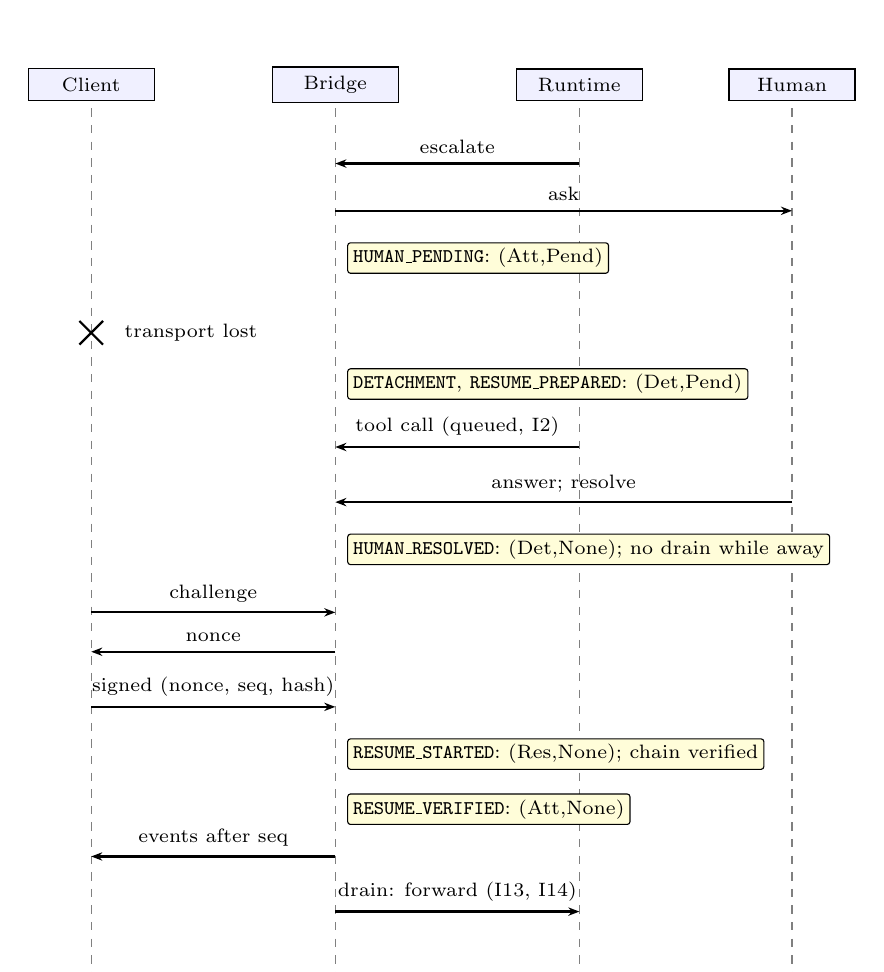
\begin{tikzpicture}[x=1cm,y=1cm,font=\scriptsize,
  msg/.style={-{Stealth[length=4pt]},thick},
  note/.style={draw,rounded corners=1pt,fill=gray!10,inner sep=2pt,align=left},
  cell/.style={draw,rounded corners=1pt,fill=yellow!15,inner sep=2pt}]
\def\cx{0}\def\bx{3.1}\def\rx{6.2}\def\hx{8.9}
\foreach \n/\x in {Client/\cx,Bridge/\bx,Runtime/\rx,Human/\hx}{
  \node[draw,fill=blue!6,minimum width=1.6cm] (\n) at (\x,0) {\n};
  \draw[dashed,gray] (\x,-0.3) -- (\x,-11.4);}
\draw[msg] (\rx,-1) -- node[above]{escalate} (\bx,-1);
\draw[msg] (\bx,-1.6) -- node[above]{ask} (\hx,-1.6);
\node[cell,anchor=west] at (\bx+0.15,-2.2) {\texttt{HUMAN\_PENDING}: (Att,Pend)};
\draw[thick] (\cx-0.15,-3) -- (\cx+0.15,-3.3) (\cx-0.15,-3.3) -- (\cx+0.15,-3) ;
\node[anchor=west] at (\cx+0.3,-3.15) {transport lost};
\node[cell,anchor=west] at (\bx+0.15,-3.8) {\texttt{DETACHMENT}, \texttt{RESUME\_PREPARED}: (Det,Pend)};
\draw[msg] (\rx,-4.6) -- node[above]{tool call (queued, I2)} (\bx,-4.6);
\draw[msg] (\hx,-5.3) -- node[above]{answer; resolve} (\bx,-5.3);
\node[cell,anchor=west] at (\bx+0.15,-5.9) {\texttt{HUMAN\_RESOLVED}: (Det,None); no drain while away};
\draw[msg] (\cx,-6.7) -- node[above]{challenge} (\bx,-6.7);
\draw[msg] (\bx,-7.2) -- node[above]{nonce} (\cx,-7.2);
\draw[msg] (\cx,-7.9) -- node[above]{signed (nonce, seq, hash)} (\bx,-7.9);
\node[cell,anchor=west] at (\bx+0.15,-8.5) {\texttt{RESUME\_STARTED}: (Res,None); chain verified};
\node[cell,anchor=west] at (\bx+0.15,-9.2) {\texttt{RESUME\_VERIFIED}: (Att,None)};
\draw[msg] (\bx,-9.8) -- node[above]{events after seq} (\cx,-9.8);
\draw[msg] (\bx,-10.5) -- node[above]{drain: forward (I13, I14)} (\rx,-10.5);
\end{tikzpicture}
\caption{The disconnect / resume / re-attach sequence, with an escalation
pending when the client disconnects. Cells are written (attachment,
human). The re-attach is a challenge and a signed request, not a token;
the human's resolution while the client is away does not drain the queue,
verification does.}\label{fig:sequence}
\end{figure}

\subsection{Threat model (STRIDE-lite)}
\label{sec:threat-model}

This subsection presents the threat model for the Bridge Contract
following the STRIDE methodology~\cite{shostack2014threat}, restricted to the
categories relevant to bridge-mediated session governance (the
``-lite'' suffix). For each STRIDE category we state whether the
Bridge Contract mitigates it, partially mitigates it, or defers to
another specification; for ``No'' rows we identify the residual-risk
owner.

\paragraph{Assets.} The Bridge Contract protects the following
assets:
\begin{itemize}[leftmargin=2em]
\item \textbf{Event log integrity.} The append-only, hash-chained
log of governance events per session (A1, I5).
\item \textbf{Resume integrity and authenticity.} The resume record
written at detach and the challenge-response that gates re-attach (I1,
I4, I5, I9, I11).
\item \textbf{Authority scope.} The set of permissions granted to
the session at attach; widening is refused, or reported when the runtime does it itself, in every cell (I3, I10).
\item \textbf{Tool-call queue.} The queue of pending tool calls
while the human dimension is pending; queue contents are part of the resume
record and of the replay (I2, I13).
\item \textbf{Session lifecycle.} The set of allowed state
transitions; $\bot$ is terminal (I6).
\end{itemize}

\paragraph{Adversaries.} The threat model considers the following
adversaries:
\begin{itemize}[leftmargin=2em]
\item \textbf{Network attacker.} Can observe and modify traffic
between client, bridge, and (in GEC-present deployments) GEC.
The contract specifies no transport binding, so this is mitigated only by a transport the deployment supplies (``Approvals and resolutions are not signed'', Table~\ref{tab:limitations}); I-SIGN-EVENT is a SHOULD without a test.
\item \textbf{Byzantine client (in scope, \S\ref{sec:scope}).} May attempt to replay captured
re-attach requests, present a history that is not a prefix of the chain,
forge requests to terminate sessions, or supply malicious JWKS
endpoints. Mitigated by I4, I9 and I11 (prefix consistency, short-lived
single-use nonce, proof of possession, rejection without state change)
and I-SIGN-JWKS (MUST NOT accept session-supplied JWKS), assuming no
registered client key is stolen (A7).
The formal model gives this adversary explicit capabilities and checks
the re-attach path against it (Appendix~\ref{app:attacker}).
\item \textbf{Byzantine bridge.} May suppress governance events or
forge events. \emph{Out of scope} (A4); mitigations are
deployment-level (external transparency logs, e.g., SCITT), and the residual risk is owned by a future revision of the contract (see the register below).
\item \textbf{Operator error.} May misconfigure timeouts, JWKS
endpoints, or authority scope. Mitigated by I-SIGN-JWKS (JWKS
source restriction), I3 (authority lock) and the timer bounds of
Section~\ref{sec:timeouts}.
\item \textbf{Compromised runtime.} The agent runtime may be
prompt-injected or otherwise compromised. It may self-approve
escalations (bypassing I2/I13 if the bridge does not authenticate
the human channel), flood the tool-call queue (mitigated by
$Q_{\max}$, I13), squat on client keys (mitigated by I11-REVOKE
revocation), or attempt to widen its own authority (reported by I3
as \texttt{observed}, not prevented). The runtime is trusted for
execution (the bridge cannot see what the runtime does with a
forwarded call), but not for authority changes: I3 and I10 ensure
the bridge's record never widens, even if the runtime's effective
authority does.
\end{itemize}

\paragraph{Trust boundaries.} The trust boundaries assumed by the
Bridge Contract are:
\begin{itemize}[leftmargin=2em]
\item \textbf{Client $\leftrightarrow$ Bridge.} Untrusted: the
client may be Byzantine, but it does not control the bridge's event log;
its misbehaviour is mitigated by I4, I9, I11 and I-SIGN-JWKS, except where it
holds a valid key (A7).
\item \textbf{Bridge $\leftrightarrow$ Agent runtime.} Trusted
under A4 (the bridge is non-Byzantine); the agent runtime is
out of scope.
\item \textbf{Bridge $\leftrightarrow$ GEC.} In GEC-present
deployments, the GEC is the sole authoritative event source
(per GAR \S 3); the bridge forwards unsigned events.
\item \textbf{Bridge $\leftrightarrow$ Audit consumer.} The audit
consumer (e.g., a SIEM feed, a SCITT transparency log) reads
events emitted by the bridge; in GEC-less deployments, the
consumer verifies the operator key binding out-of-band
(I-SIGN-EVENT).
\end{itemize}

\paragraph{STRIDE coverage.} Table~\ref{tab:threats} maps STRIDE
categories to Bridge Contract invariants. ``S'' = Spoofing;
``T'' = Tampering; ``R'' = Repudiation; ``I'' = Information
Disclosure; ``D'' = Denial of Service; ``E'' = Elevation of
Privilege.

\begin{table}[htbp]
\centering
\caption{STRIDE coverage: threats the Bridge Contract mitigates
(or does not), with residual-risk owner for unmitigated rows.}
\label{tab:threats}
\small
\begin{tabularx}{\columnwidth}{l >{\raggedright\arraybackslash}X >{\raggedright\arraybackslash}X >{\raggedright\arraybackslash}X}
\toprule
\textbf{STRIDE} & \textbf{Threat} & \textbf{Mitigated by BC?} & \textbf{Residual-risk owner} \\
\midrule
S & Authority spoofing (forged or widened scope) & Partial (I3 observed, not enforced, when the runtime widens its own authority; a forwarded call in (Att,None) is not scope-checked; I10 for the bridge's record) & Runtime; deployment operator (Table~\ref{tab:limitations}) \\
S & JWKS endpoint spoofing & Yes (I-SIGN-JWKS, MUST; by inspection only, Table~\ref{tab:limitations})\textsuperscript{a} & --- \\
S & Re-attach spoofing & Yes (I11 proof of possession) & Key custody (A7): deployment \\
T & Event log tampering (edit or reordering of events inside the log) & Yes (A1, I5) & --- \\
T & Truncation of the log, or rewriting of its last events & No without a head held outside the log (I-CHECKPOINT anchor) & Bridge operator (storage integrity, external head) \\
T & Tampering with the history presented at re-attach & Yes (I4 prefix check, I5) & --- \\
T & Forged or injected approval, resolution or escalation on an unauthenticated transport (these ops carry no signature) & No: they are transport-authenticated (Appendix~\ref{app:wire-format}) & Transport binding; deployment operator \\
T & Tampering during storage write & Partial (I12, I5) & Bridge operator (storage integrity, A1) \\
T & Replay of queued side effects after detach or crash & Yes (I13), with a cooperating runtime & Runtime must honour idempotency keys \\
R & Agent repudiation & Partial (I5 + I-SIGN-EVENT) & GEC if present; otherwise bridge operator \\
R & Bridge repudiation (a Byzantine bridge is out of scope, A4) & Partial (I5 + I-SIGN-EVENT + I-CHECKPOINT; both SHOULD, not in the baseline; the reference bridges keep no external head and the Rust crate emits no checkpoints) & External transparency log (SCITT) \\
\textbf{I} & \textbf{Disclosure of the resume record and of the replay} & \textbf{Partial} & \textbf{Bridge operator (encryption at rest and in transit per \S\ref{sec:limitations})} \\
I & Event log information disclosure & No & Bridge operator (deployment-level access control) \\
I & Tool-call queue information disclosure & No & Bridge operator (queue contents in the log and the replay; mitigate via encryption) \\
D & Detach timeout exhaustion & Partial (L1 bounds detachment and gives no availability; Table~\ref{tab:limitations}) & Bridge operator; deployment (Table~\ref{tab:limitations}) \\
D & Human timeout exhaustion & Yes (L2) & --- \\
D & Session termination by forged re-attach attempts or by holding the nonce book & Partial (I11: a rejected request changes no cell; but a caller without a key that holds the live-nonce limit refuses a detached client every challenge until $T_{\text{detach}}$ ends the session, Section~\ref{sec:invariants-token-auth}) & Rate-limiting or authentication of the transport in front of \texttt{challenge}: bridge operator \\
D & Denying a genuine re-attach by flooding \texttt{challenge} or the log without a key & Partial (I11 (f), (g): a live nonce is never evicted, and the failures before authentication recorded between two verifying requests are bounded; a replayed authentic request is recorded and restores that allowance, so the log grows with the caller's effort; the limit of live nonces can still be held, delaying a new challenge by up to $T_{\text{nonce}}$ each time) & Rate-limiting or authentication of the transport in front of \texttt{challenge}: bridge operator \\
D & Bridge restart & Partial (I12, Section~\ref{sec:recovery}) & Bridge operator (HA, replication) \\
E & Authority drift in any cell & Partial (I3 observed; I10 for the bridge's record) & Runtime; deployment operator (Table~\ref{tab:limitations}) \\
E & Privilege escalation by presenting a stale or forged history & Yes (I4, I11) & --- \\
S & Replay of a captured re-attach or join request & Yes (a captured request cannot be replayed: I11 single use, I9 lifetime, and a nonce issued for a key that was not registered never verifies) & --- \\
S & Theft of a client key & Partial (I11-REVOKE: operator can revoke) & Key management: deployment (operator must sign revocation) \\
\bottomrule
\end{tabularx}
\end{table}

\noindent\textsuperscript{a} I-SIGN-JWKS is vacuous in GEC-present deployments (the GEC provides the JWKS endpoint).

\paragraph{Residual-risk register.} Rows marked ``Partial'' or
``No'' have residual risk owned by:
\begin{itemize}[leftmargin=2em]
\item \textbf{Bridge operator (deployment).} Configures
persistence, HA, encryption at rest, access control. Not in scope
for BC.
\item \textbf{GEC (if present).} Authoritative event source per
GAR; bridge forwards events in GEC-present deployments.
\item \textbf{External transparency log (SCITT).} For
non-repudiation of bridge events in GEC-less deployments where
the bridge operator is potentially untrusted.
\item \textbf{Future revision of BC.} For concerns explicitly
deferred (multi-hop composition, Byzantine bridge, partial
detach), the residual risk is owned by a future revision of this
specification.
\end{itemize}

\paragraph{Out-of-scope threats.} The following STRIDE-relevant
threats are explicitly out of scope for this document (see
\S\ref{sec:scope}):
\begin{itemize}[leftmargin=2em]
\item Bridge replication and failover (D): deployment-level.
\item Network partition / partial detach (D, T): not modelled.
\item True concurrency on the same session (T, R): events are
serialised (A5); interleavings are covered by the product machine only.
\item Byzantine bridge (T, R, I): A4 assumes non-Byzantine bridge.
\item Multi-hop composition (S, T, E): BC $\circ$ BC not modelled.
\end{itemize}

% ================================================================================

\section{Reference Implementation Notes}
\label{sec:impl}
% ================================================================================

This section sketches how a generic agent-runtime bridge can implement
the Bridge Contract without requiring changes to AGTP, GAR, or PACE.
The implementation is on the bridge side only.

\paragraph{State store.} The bridge maintains a state store keyed by
\texttt{Session-ID}, mapping each session to its current state, its
Session Identity Descriptor, its tool queue, and its event log. The store
is private to the bridge; AGTP, GAR, and PACE components do not read
from it directly.

\paragraph{Event emitter.} The bridge emits events in a JSON shape that
is compatible with GAR's SAR record (causal ordering, hash chaining).
In a GEC-present deployment, the events are forwarded to the GEC for
signing; the GEC remains the sole authoritative source. In a GEC-less
deployment (Definition~\ref{def:gecless}), the bridge SHOULD sign the
events itself with an operator key whose JWKS endpoint is published
through an out-of-band channel bound to the operator's deployment
identity (GAR \S 6.1, Invariants I-SIGN-EVENT and I-SIGN-JWKS). The bridge MUST NOT accept a
JWKS endpoint learned from session-supplied metadata.

\paragraph{Challenge store.} The bridge keeps, per session, a small
volatile set of live challenge nonces with their issue times and a
used flag (I9, I11). It is not durable: a restart voids every nonce and
clients ask again. The registry of client keys is scoped to a session and is rebuilt from the
log, which records each key's scheme tag and public key, and a restart
compares the stored registry with it.
Everything else needed to resume, the chain and the resume record, is in
the log (I12). The Python reference bridge and the Rust crate verify
resume requests signed with Ed25519 or ECDSA P-256 (clients and fixtures
sign), and their key registries
hold a scheme tag and public keys only, so the evidence exercises proof of possession against verification
material alone.

\paragraph{Tool-call queue.} While the human dimension is pending,
the bridge maintains a bounded queue of pending tool calls, each with
an idempotency key. Each enqueued call emits
\texttt{TOOL\_CALL\_QUEUED}. Once the client is attached and no
escalation is outstanding, the queue is drained in arrival order, each
call re-validated against the current scope and approval (I13).

\paragraph{Durable log and recovery.} The event log is written with a
commit barrier before any state change or acknowledgement (I12). On
start the bridge replays each log, verifies the chain, and recovers
sessions as detached (Section~\ref{sec:recovery}).

\paragraph{Findings from integration.} Mapping the contract onto a real
product (Termenbox ACP workspaces: the server is the bridge, the browser
the client, the agent a child process on stdio) found, as reported by the
author (the product is closed source and no reader can check this), problems that the
paper's own evidence could not, because the evidence came from the same
author reading the same text. A resume token minted at detach and
superseded by every later change while the client was away, could not
reach a client that vanished abruptly, and I9 then terminated the
session when it expired; the model had one client where a product owner
has several devices attached at once; the bridge sees an approval
request, not tool execution, so I2 as first worded promised more than a
bridge can see; an agent announces its own mode changes, which a bridge
can observe and revert but not prevent; and the independent defaults for
the human and call timers ended work that a mobile owner expects to
survive. Each, as reported, led to a change of the specification, not of the product
(challenge-response resume, a client set, answer binding, the
coverage limits of I2 and I3, derived timers). The same author wrote
both sides, which limits what this shows.

\paragraph{Reference implementation.} A reference implementation is
provided in the conformance test suite (Section~\ref{sec:conformance}).
The suite includes a \texttt{Bridge} class that the suite and its mutants
exercise against invariants $I_1, \ldots, I_{15}$; known deviations are
recorded in the limitations register (Table~\ref{tab:limitations}). It also has a
\texttt{SessionIdentity}, \texttt{Event}, and re-attach request data
model. A second implementation in Rust
(\texttt{supplementary/rust-bridge/}), written from Sections~4 and~5
rather than ported from the Python code (though it shares comments, error
texts and the key format with it), runs the same JSON vectors except
V52--V54, V88 and V89, which expect checkpoint events the crate does not
emit; it
has the same author, so it shows consistency of one reading of the
text. A runtime such as
Termenbox~\cite{termenbox}, a self-hosted web terminal for AI coding agents
(the author's project; see the note on evidence at the front of this
document), is one
example of a runtime that could implement the Bridge Contract; the
contract is deliberately implementation-agnostic and does not depend
on any particular runtime substrate.

% ================================================================================

\section{Conformance Suite}
\label{sec:conformance}
% ================================================================================

The reference test suite comprises the pytest cases in
\texttt{conformance\_suite.py} (Python 3.10, pytest 9.1.1, Hypothesis
6.168.5; \texttt{requirements.txt}): deterministic tests T1--T158 (some
parametrised over the active cells), and property-based tests
T8--T10 that run random action sequences of up to 40 operations (30 for T10), % count-ok
including a second device, restarts and clock jumps. Every invariant
I1--I15 is exercised (Table~\ref{tab:invariant-independence}). The tests
run the reference \texttt{Bridge} class through its public API only, and
no deterministic test passes by swallowing a refusal
(\texttt{BridgeError}); the property-based driver treats refusals as
expected outcomes and checks the invariants after every action. I8 is
tested through a transport-reported replay flag. I-SIGN-EVENT and
I-SIGN-JWKS concern keys and external services outside the reference
bridge and have no test or vector; I-SIGN-JWKS is a MUST, so a claim
of conformance to it rests on inspection of how the bridge obtains
keys, not on a test, and it has no mutant. I-CHECKPOINT local emission
and field names are tested by T63--T66 and by vectors V52--V54, V88 and
V89, which expect the \texttt{CHECKPOINT} event and run on the Python bridge
only, because the Rust crate has no emission (its runner skips vectors that
require it); external anchoring (SCITT submission) has no test.

\textbf{Important caveat.} The pytest suite tests the
reference \texttt{Bridge} class only and is not an interop test. The
language-neutral vectors (\S\ref{sec:test-vectors}) are the interface for
other implementations; so far they have been run against the Python reference bridge
and the Rust crate, both by the same author; no third-party implementation exists.
Table~\ref{tab:tests} maps the tests to the invariants they exercise;
Table~\ref{tab:traceability} (Appendix~\ref{app:traceability}) traces each
invariant to its TLA+ property, tests, vectors and mutants.

% GENERATED by supplementary/tests_table.py --emit-tex; do not edit.
\begin{longtable}{p{0.12\columnwidth} p{0.2\columnwidth} p{0.58\columnwidth}}
\caption{Tests and the invariants they exercise.}\label{tab:tests}\\
\toprule
\textbf{Tests} & \textbf{Invariants} & \textbf{What they check} \\
\midrule
T1, T7, T10, T11, T19c--T22, T52 & I1, I4, I5, I7, I11 &
Detach emits \texttt{RESUME\_PREPARED} before the cell changes; an
authentic re-attach goes through RESUMING, emits \texttt{RESUME\_VERIFIED}
only on RESUMING $\to$ ATTACHED, and replays exactly the events after the
acknowledged prefix; a history that is not a prefix of the chain is
refused without changing state; a request while RESUMING is refused;
disconnect during resume returns to DETACHED; a broken chain during
resume quarantines the session (T22--T22d); a client resumes however long it was away (T10, T31),
which a held token of limited lifetime could not guarantee. \\
T2, T25 & I2, I13 &
Calls queue under $\textsc{Pend}$ in every attachment, are forwarded only
in $(\textsc{Att},\textsc{None})$, and drain with one
\texttt{TOOL\_CALL\_DRAINED} each. \\
T3, T12, T15, T15b, T56 & I3, I10 &
Widening is rejected in every active cell and emits
\texttt{AUTHORITY\_EXTENSION\_REJECTED}; a widening the runtime announces
itself is reported with source \texttt{observed}, the bridge's record is
unchanged and a revert is requested; narrowing is allowed everywhere as
one event, and a narrowing made while the client was away does not fail
its re-attach. \\
T4, T40 & I6 &
Every mutating operation fails after termination, including across a
restart. \\
T5 & I5 &
A tampered or forged event is detected by chain verification. \\
T6, T26--T29, T30b--T30e & L1, L2, I6 &
Detach and human timeouts, their anchors, simultaneous expiry, and the
zero-timeout edge case; a human wait that outlasts $T_{\text{detach}}$
only while the client is attached; the cumulative cap across episodes,
across restarts and not counting time attached or resuming. \\
T8, T9 & A2, I1--I3, I5, I6, I10, I11, I14, I15 &
Property-based: gap-free sequences, and the invariants hold after every
action of a random sequence, with the cell and the client set equal to
the fold of the log. \\
T13, T13b, T30, T31 & I9, I11 &
An expired nonce is rejected without terminating and without revealing
more than a bad signature; the timer bounds are enforced and derived. \\
T22--T22d, T38 & I5, I12 &
A chain failure after an accepted re-attach, and a recovery failure,
quarantine the session: the failure is recorded, nothing terminates, no
operation or timer acts on it, a restart does not lift it, and a
presenter without a registered key cannot cause it. \\
T57--T59b (vectors V33--V37) & I2, I14 &
A call outside an escalation is refused by default; under the queue
variant it is held until answered after re-attach; under the forward
variant only allowlisted, in-scope permissions are forwarded; while an
escalation is pending nothing is forwarded under any variant. \\
T60--T60d (vectors V38--V40) & I12, I13 &
A drained call awaits delivery and completion; an unacknowledged call is
forwarded again after a restart, with the same key and without a second
drain, only in $(\textsc{Att},\textsc{None})$. \\
T61 & A6, I2 &
Escalations coalesce: a second one is audited, changes no cell and does
not restart $T_{\text{human}}$; one resolution ends them all. \\
T62 (vector V43) & A6 &
A host clock that went backwards across a restart counts as no time
elapsed, and committed timestamps never decrease. \\
T43 (vector V41) & I13, I14 &
An approval given while the client is away lapses after
$T_{\text{approve}}$: the call expires on re-attach and is not
forwarded. \\
T19 (vector V42) & I11 &
A request refused as \texttt{resume\_in\_progress} spends its nonce. \\
T14 & I10 &
\texttt{scope\_version} increments on each strict narrowing; no-op
narrowing is rejected. \\
T16 & I8 &
A transport-reported 0-RTT replay is rejected, cell unchanged. \\
T17--T19b, T51 & I11 &
The signature covers every field; the session, a nonce and the chain (a
bearer) are not enough; a consumed, unknown or foreign-session nonce is
never accepted, and an authentic request spends its nonce even when
rejected later; issuing a challenge writes nothing to the log. \\
T23, T24 & I2, I13 &
Human resolution while detached keeps the queue and drains only after
verification. \\
T32--T40 & I7, I12 &
A failed append changes nothing; nothing is forwarded before its drain
event is durable; restart recovers every cell as detached with an empty
client set, voids outstanding nonces, restarts timers, applies elapsed
timeouts, and fails on a broken chain or a lost key registry. \\
T41--T45 & I13 &
Idempotency keys, queue limit, call expiry, approval expiry, and
revalidation of the current scope at drain; the resume record carries the
queue. \\
T47--T50 & I15 &
A second device joins an attached session; only the last departure
detaches; an added key resumes, an unregistered one is refused, and
registration needs a connected client; a scope narrowed from one device
reaches the other through the replay. \\
T119--T123 (vectors V105--V108) & I15 &
A client registration needs a fresh signature by a connected, unrevoked
key over the operation, session, new key and nonce: unsigned, forged,
other-operation, replayed, expired and revoked-key requests are refused with
a named reason and commit nothing; the signed bytes are pinned by known
answers. \\
T124--T125 & I11 &
The attach proof of possession is the bytes of the tagged tuple that names
the bridge, the session and the key with its scheme tag, pinned by known
answers that a changed field does not verify against; the wire constructors
for attach and client registration carry the scheme. \\
T126 (vector V109) & I11 (a) &
\texttt{challenge} refuses an unknown, a terminated and a quarantined
session with one text that names neither the session nor its state. \\
T127 (vector V110) & I11 (a) &
\texttt{reattach} and \texttt{join} refuse an unknown, a terminated and a
quarantined session with one text that names neither the session nor its
state. \\
T128 (vector V111) & I11-REVOKE &
A key revoked for compromise while its re-attach is verified is not the
attached client afterwards: the re-attach is abandoned (detached, resume
record rewritten) and \texttt{complete\_resume} refuses; a soft revocation
leaves the verification alone. \\
T138--T140 (vectors V121--V126; \texttt{vectors/bytes\_kat.json}) & I-OPERATOR &
An operator signature is bound to the bridge identity and to the log
position (sequence and hash of the last event) at signing: one made for
another bridge, or at an earlier or other position, is refused for a
revocation, a key addition and a termination, and the signed bytes and
signatures are pinned by known answers that a changed field does not verify
against. \\
T141--T142 (vectors V127, V128) & I11, I15 &
A re-attach on an attached session is refused as
\texttt{already\_attached} (rejected, nonce spent, no change of cell) and join
is the way in; the reason is given only to an authentic request, so an
unauthenticated one still gets its own reason. \\
T129--T130 (vectors V112, V113) & I14 &
The approval hash covers the tool and the permission as well as the
content, so approving the arguments of one call does not release another
under a different tool name; the bridge retains the hashed request in the
log and forwards exactly that request, also when it forwards it again after
a restart. \\
T131 (vector V114) & rule Q &
A log that cannot be replayed (no \texttt{ATTACHED} first, or one
without its fields) quarantines its own session only; the other sessions are
recovered and nothing is appended to the malformed log. \\
T132 & I11-REVOKE &
Unsigned revocation requests are written up to a bound per session and
refused past it without a log entry; a signed revocation restores the
budget. \\
T133 & Appendix B &
The reference wire server calls an authentication hook for each unsigned
op and refuses it as \texttt{unauthenticated} on a false answer; signed ops
do not reach the hook. \\
T53--T55 & I14 &
A matching answer drains and the event repeats the hash; a changed view,
a denial or no answer block the forward; the first answer is final. \\
T63--T66, T63b (vectors V52--V54, V88, V89; Python only) & I-CHECKPOINT &
A \texttt{CHECKPOINT} is emitted after the configured number of events
since the last checkpoint and after $T_{\text{cp}}$; its root matches the
recomputed Merkle root; the receipt is optional. The vectors expect the
\texttt{CHECKPOINT} event in the log. \\
T97--T100 (vectors V86, V87) & I11 (f), (g) &
Keyless challenges cannot evict a live nonce and are refused once the
limit is reached; spent and expired nonces make room; unauthenticated
rejections are recorded only up to the bound and are refused uniformly;
the genuine re-attach is accepted after both floods. \\
T101--T104 (vectors V90--V94; \texttt{vectors/bytes\_kat.json}) & I11, I5 &
RFC~8785 known answers (non-ASCII strings, escapes, UTF-16 key order,
numbers, inputs with no canonical form); pinned event and content
hashes; the exact bytes and Ed25519 signature of a re-attach and a join
proof; a proof made for the other operation, for another key id, over
the untagged tuple or without the key id is refused as
\texttt{bad\_signature}. \\
T105--T112, T143 (vectors V95, V96, V102--V104, V129) & I11, I12 &
A key identifier is scoped to its session: a second, validly granted
session that reuses it neither replaces the first session's key nor can
re-attach to the first session, and the owner is not locked out;
\texttt{ATTACHED}, \texttt{CLIENT\_ADDED} and \texttt{OPERATOR\_ADD\_KEY}
carry the scheme tag and public key; recovery repairs the registry from
the log, which is the source of truth: an entry that differs is replaced, one
the log does not record (a crash between the registry write and the event
commit) is dropped, a missing one is written back, and
\texttt{BRIDGE\_RECOVERED} names the keys repaired; a refused append leaves
no registry entry. \\
T113--T118 (vectors V97--V101) & I-GRANT, I11 &
Attach needs a proof of possession by the registered key, under its own
domain tag and bound to the bridge, the session and the key; a missing
proof, a proof by another key and a proof made for another bridge are
refused as \texttt{possession\_invalid}; the grant binds the public key
and the bridge, so a grant seen in transit cannot be used with another
public key under the same key identifier or at another bridge
(\texttt{grant\_invalid}). \\
T67--T69, T75, T76, T86, T87 & I11-REVOKE, I11 &
A soft revocation does not detach an active client; a hard revocation
detaches the revoked key's client and keeps the others connected; a
revoked key is refused on re-attach, also when revoked after its
challenge; two-phase rotation; revoked keys survive a restart. \\
T70--T74, T88, T89 & I11-REVOKE, I6 &
Revoking the last key enters \texttt{key\_exhausted}; client operations are
refused there; the operator adds a recovery key or terminates; the state
and the recovery key survive a restart; refused revocations commit
nothing. \\
T134--T137 (vectors V115--V120) & I11-REVOKE, L1, L2 &
The timers of a \texttt{key\_exhausted} session keep running: it ends
after $T_{\text{detach}}$ (a client operation on an expired session reports
the end, not the exhaustion), an operator key must arrive before the bound,
a restart treats the session like any other and restarts $T_{\text{detach}}$,
a pending escalation times out, and a session whose revoked key is still
connected detaches on transport loss and then ends. \\
T77--T81 & I-GRANT &
An attach is accepted only with a valid grant, which is bound to the
session, scope lineage and key and carries its own domain tag; without
a grant verifier every attach is refused. \\
T82--T85 & I11 &
P-256 proof of possession is accepted and forged proofs are rejected; a
scheme tag is not interchangeable; a known-answer signature from an
independent signer verifies; a server takes only a client's public key. \\
T144 & I11 &
A test-only further scheme tag is accepted at attach through the
pluggable verifier, with no change to the bridge, and refused where the
verifier lacks the tag (extension, Section~\ref{sec:ext-schemes}). \\
T145, T146 (vector V130) & I11-REVOKE, I6 &
An unsigned terminate of a key-exhausted session is refused and commits
nothing; only the operator's signed termination ends it. The refusal
defers to the timers (an expired session is found ended) and to
quarantine (the operator's way out of quarantine stays open). \\
T147 (vector V131) & I11, I15 &
A re-attach naming an unregistered key and one with a bad signature get
the same refusal, so the answer does not list the registered key ids;
the log keeps the true reason. \\
T148--T151 (vector V132) & wire, I-OPERATOR &
The wire server creates a session from an \texttt{attach} message
(refusing a missing grant or proof by name), answers \texttt{resolve} and
\texttt{extend} (the scope in force, a requested revert), verifies the
operator events from the message and names their refusals, and names the
key-exhausted refusal of a bare terminate. \\
T152--T155 (vectors V133, V134) & I11, I11g, I15, wire &
Two sessions on one bridge that hold the same client key share
nothing but the bridge: a nonce issued for one session is unknown to the
other for a re-attach, a join and a registration, and spent by neither
refusal; the budgets of challenges, unauthenticated rejections and
revocation requests are kept per session and are not restored by a
request in another; a tool call key means a call only in its session,
across a restart; every unsigned wire op is asked of the authentication
hook with the message that names its session, and a hook that accepts one
session's caller does not open another. \\
T156--T158 & I11, I14 &
Cases the mutation check could not see while its scratch copies failed
on their own: recovery leaves the registry of a quarantined session as
found; ATTACHED records the scheme of the first key, so a lost entry is
written back with it; a call held while no client is attached carries the
hash of the call a client is shown. \\
T90--T96 (vectors V75--V85) & I-OPERATOR &
Revocation, key addition and termination require a valid operator
signature bound to the session, key and operation; a bridge without an
operator verifier refuses them; the signature is logged and survives
recovery; the operator domain tags separate the signatures. \\
T46 & --- &
The derived view of named states. \\
\bottomrule
\end{longtable}


\paragraph{Mutation check.} A passing suite shows little unless it can
fail. \texttt{mutation\_check.py} applies one-line mutants to the
reference bridge, at least one per invariant I1--I15 and one for the
timer bounds (for example: mutate before append, drop the previous hash,
skip the prefix check, spend a nonce only on success, let an expired
nonce terminate, forward on a mismatching answer hash, detach on a
partial departure, record an observed widening), and requires the suite
to fail on each. A mutant is killed only when pytest exits with code 1
and reports a failed test; a collection, import or syntax error is
reported as an error, not a kill, and a patch that changes nothing must
survive (a control). The script prints the failing tests and whether one
of them carries the mutant's invariant tag in its docstring (kills by a
test with no such tag are listed). Every mutant is killed; the script
exits non-zero otherwise. I-SIGN-JWKS, which is checked by inspection, has none. The mutants include the eviction of a live nonce by a further challenge
and the unbounded logging of unauthenticated failures (I11 (f), (g)), the
dropping of the operation tag or of the key id from the re-attach and join
proof, and, in the canonical encoding, the escaping of non-ASCII text,
code point instead of UTF-16 key order, the printing of an integral float
as \texttt{1.0} and the acceptance of an integer beyond $2^{53}$; and
the count trigger of I-CHECKPOINT
(counting the whole log instead of the events since the last
checkpoint). The Rust crate has a separate, smaller harness,
\texttt{mutation\_check\_rust.py}, which applies one-line mutants to
signature verification, nonce spend, expiry and replay, revoked-key
rejection, the registered-key check, the acknowledged-prefix check, the
hash chain, the operation tag and key id of the resume proof and the
canonical encoding, and requires \texttt{cargo test} to fail on each. It is
a sample of the highest-value rules, not one mutant per invariant; the
mutation evidence for I1--I15 as a whole is on the Python bridge.

\paragraph{Reproducibility.} To reproduce, from
\texttt{paper/supplementary}:

\begin{lstlisting}[language=,basicstyle=\ttfamily\small,frame=single,backgroundcolor=\color{codebg},breaklines=true]
$ python3 -I -m pytest conformance_suite.py -q     # all tests passed
$ python3 -I mutation_check.py                     # every mutant killed
$ python3 -I mutation_check_rust.py                # every Rust mutant killed
$ python3 -I run_vectors.py                        # all vectors passed (V01-V134)
$ python3 -I run_vectors.py --wire                 # wire roundtrip smoke test
$ (cd rust-bridge && cargo test)                   # all vectors on MemStorage and FileStorage
\end{lstlisting}

\noindent The same commands are listed in \texttt{paper/supplementary/REPRODUCE.md}
for readers who prefer a shell-readable copy. The TLC runs are described in
Appendix~\ref{app:formal}. The commands assume a virtual environment in
which \texttt{requirements.txt} is installed (\texttt{python3 -I} ignores
packages installed per user). The runtime requirements of the Python
suite are Python $\geq 3.10$, \texttt{pytest} $\geq 8.0$,
\texttt{hypothesis} $\geq 6.0$, \texttt{cryptography} and
\texttt{jsonschema} (the schema check), with the RFC~8785 encoder bundled
as \texttt{jcs.py}; \texttt{requirements.txt} lists them.

\paragraph{Conformance language and unit.} ``Conformance'' in this
specification is defined at the \emph{bridge} level: a bridge
implementation is conformant if it satisfies all MUST invariants
($I_1, \ldots, I_{15}$, I11-REVOKE, I-GRANT, I-OPERATOR and
I-SIGN-JWKS) for every session it
mediates. Conformance is \emph{not} defined at the session,
deployment, or runtime level; a non-conformant bridge may still
mediate conformant sessions, but its emitted event log is not a
trustworthy audit feed. The tests and vectors provided with this
document check the Python reference bridge and the Rust crate, written by one author; they are not a
third-party interop campaign.

\subsection{Test vectors}\label{sec:test-vectors}

The vectors are language-neutral JSON files in
\texttt{supplementary/vectors/} (\texttt{V01.json}--\texttt{V134.json}).
Each gives a session, an optional configuration, a list of actions and
the expected committed event kinds, final cell and scope version; the
file \texttt{vectors/README.md} defines the schema. The table below is
generated from those files by \texttt{run\_vectors.py --emit-tex} and
checked for staleness by \texttt{run\_vectors.py --check-paper}; a
trailing \texttt{!} marks an action the bridge must refuse. The Python
reference bridge passes all of them (\texttt{python3 -I run\_vectors.py}),
and the Rust crate in \texttt{supplementary/rust-bridge/} runs the same
files, except V52--V54, V88 and V89, which expect checkpoint events the
crate does not emit.

Table~\ref{tab:vectors} lists them.

% GENERATED by supplementary/run_vectors.py --emit-tex; do not edit.
\begingroup\scriptsize\setlength{\tabcolsep}{3pt}
\begin{longtable}{@{}p{0.05\columnwidth} >{\raggedright\arraybackslash}p{0.17\columnwidth} >{\raggedright\arraybackslash}p{0.21\columnwidth} >{\raggedright\arraybackslash}p{0.38\columnwidth} >{\raggedright\arraybackslash}p{0.11\columnwidth}@{}}
\caption{Language-neutral test vectors.}\label{tab:vectors}\\
\toprule
\textbf{ID} & \textbf{Scenario} & \textbf{Actions} & \textbf{Expected event kinds} & \textbf{Final cell} \\
\midrule
\endfirsthead
\toprule
\textbf{ID} & \textbf{Scenario} & \textbf{Actions} & \textbf{Expected event kinds} & \textbf{Final cell} \\
\midrule
\endhead
\texttt{V01} & Detach while a human is pending, then authenticated resume & \texttt{escalate; disconnect; reattach} & \texttt{ATTACHED, HUMAN\_\allowbreak{}PENDING, DETACHMENT, RESUME\_\allowbreak{}PREPARED, RESUME\_\allowbreak{}STARTED, RESUME\_\allowbreak{}VERIFIED} & Att/Pend \\
\texttt{V02} & A rejected re-attach (hash-mismatch) does not terminate; a second re-attach succeeds & \texttt{disconnect; reattach(hash-mismatch)!; reattach} & \texttt{ATTACHED, DETACHMENT, RESUME\_\allowbreak{}PREPARED, RESUME\_\allowbreak{}REJECTED, RESUME\_\allowbreak{}STARTED, RESUME\_\allowbreak{}VERIFIED} & Att/None \\
\texttt{V03} & RESUME\_\allowbreak{}VERIFIED marks Res to Att, not entry to Res & \texttt{disconnect; reattach(no-complete); complete\_\allowbreak{}resume} & \texttt{ATTACHED, DETACHMENT, RESUME\_\allowbreak{}PREPARED, RESUME\_\allowbreak{}STARTED, RESUME\_\allowbreak{}VERIFIED} & Att/None \\
\texttt{V04} & Widening rejected in (Det,Pend) & \texttt{disconnect; escalate; extend([read:docs,exec:shell,exec:sudo])!} & \texttt{ATTACHED, DETACHMENT, RESUME\_\allowbreak{}PREPARED, HUMAN\_\allowbreak{}PENDING, AUTHORITY\_\allowbreak{}EXTENSION\_\allowbreak{}REJECTED} & Det/Pend \\
\texttt{V05} & An expired nonce is rejected and does not terminate; a fresh one resumes & \texttt{disconnect; challenge; advance(60); reattach(n1)!; reattach} & \texttt{ATTACHED, DETACHMENT, RESUME\_\allowbreak{}PREPARED, RESUME\_\allowbreak{}REJECTED, RESUME\_\allowbreak{}STARTED, RESUME\_\allowbreak{}VERIFIED} & Att/None \\
\texttt{V06} & Scope versioning; narrowing only & \texttt{narrow([read:docs]); narrow([]); narrow([read:docs])!} & \texttt{ATTACHED, AUTHORITY\_\allowbreak{}NARROWED, AUTHORITY\_\allowbreak{}NARROWED, AUTHORITY\_\allowbreak{}EXTENSION\_\allowbreak{}REJECTED} & Att/None, sv=2 \\
\texttt{V06b} & The scope is recorded as a sorted set: order and repetition do not change the authority hash & \texttt{disconnect} & \texttt{ATTACHED, DETACHMENT, RESUME\_\allowbreak{}PREPARED} & Det/None \\
\texttt{V06c} & A narrowing that is not strict is refused as not\_\allowbreak{}a\_\allowbreak{}strict\_\allowbreak{}narrowing, whether it repeats the scope or widens it & \texttt{narrow([exec:shell,read:docs,read:docs])!; narrow([read:docs,exec:shell,admin])!; narrow([read:docs])} & \texttt{ATTACHED, AUTHORITY\_\allowbreak{}NARROWING\_\allowbreak{}REJECTED, AUTHORITY\_\allowbreak{}EXTENSION\_\allowbreak{}REJECTED, AUTHORITY\_\allowbreak{}NARROWED} & Att/None, sv=1 \\
\texttt{V07} & A nonce that was used once is never accepted again & \texttt{disconnect; reattach(as:n1); disconnect; reattach(n1)!} & \texttt{ATTACHED, DETACHMENT, RESUME\_\allowbreak{}PREPARED, RESUME\_\allowbreak{}STARTED, RESUME\_\allowbreak{}VERIFIED, DETACHMENT, RESUME\_\allowbreak{}PREPARED, RESUME\_\allowbreak{}REJECTED} & Det/None \\
\texttt{V08} & A request without a valid signature is rejected & \texttt{disconnect; reattach(bad-signature)!} & \texttt{ATTACHED, DETACHMENT, RESUME\_\allowbreak{}PREPARED, RESUME\_\allowbreak{}REJECTED} & Det/None \\
\texttt{V09} & A reported 0-RTT replay is rejected & \texttt{disconnect; reattach(replay)!} & \texttt{ATTACHED, DETACHMENT, RESUME\_\allowbreak{}PREPARED, RESUME\_\allowbreak{}REJECTED} & Det/None \\
\texttt{V09b} & A request the transport flags as a replay has spent its nonce: the same request is refused without the flag & \texttt{disconnect; reattach(as:r1,replay)!; reattach(again:r1)!; reattach} & \texttt{ATTACHED, DETACHMENT, RESUME\_\allowbreak{}PREPARED, RESUME\_\allowbreak{}REJECTED, RESUME\_\allowbreak{}REJECTED, RESUME\_\allowbreak{}STARTED, RESUME\_\allowbreak{}VERIFIED} & Att/None \\
\texttt{V10} & Restart recovers a pending session as detached, then it resumes & \texttt{escalate; tool\_\allowbreak{}call(k1); restart; reattach} & \texttt{ATTACHED, HUMAN\_\allowbreak{}PENDING, TOOL\_\allowbreak{}CALL\_\allowbreak{}QUEUED, BRIDGE\_\allowbreak{}RECOVERED, DETACHMENT, RESUME\_\allowbreak{}PREPARED, RESUME\_\allowbreak{}STARTED, RESUME\_\allowbreak{}VERIFIED} & Att/Pend \\
\texttt{V11} & Restart applies an elapsed human timeout & \texttt{escalate; restart(500)} & \texttt{ATTACHED, HUMAN\_\allowbreak{}PENDING, BRIDGE\_\allowbreak{}RECOVERED, DETACHMENT, RESUME\_\allowbreak{}PREPARED, HUMAN\_\allowbreak{}TIMEOUT, TERMINATION} & Terminated \\
\texttt{V12} & Human resolves while detached: queue drains only after resume (Rule D) & \texttt{disconnect; escalate; tool\_\allowbreak{}call(k1); resolve; reattach} & \texttt{ATTACHED, DETACHMENT, RESUME\_\allowbreak{}PREPARED, HUMAN\_\allowbreak{}PENDING, TOOL\_\allowbreak{}CALL\_\allowbreak{}QUEUED, TOOL\_\allowbreak{}CALL\_\allowbreak{}ANSWERED, HUMAN\_\allowbreak{}RESOLVED, RESUME\_\allowbreak{}STARTED, RESUME\_\allowbreak{}VERIFIED, TOOL\_\allowbreak{}CALL\_\allowbreak{}DRAINED} & Att/None \\
\texttt{V12b} & A resolution with no escalation pending is refused & \texttt{resolve!; disconnect; resolve!} & \texttt{ATTACHED, DETACHMENT, RESUME\_\allowbreak{}PREPARED} & Det/None \\
\texttt{V13} & Queue limit and idempotency keys & \texttt{escalate; tool\_\allowbreak{}call(k1); tool\_\allowbreak{}call(k1); tool\_\allowbreak{}call(k2); tool\_\allowbreak{}call(k3)} & \texttt{ATTACHED, HUMAN\_\allowbreak{}PENDING, TOOL\_\allowbreak{}CALL\_\allowbreak{}QUEUED, TOOL\_\allowbreak{}CALL\_\allowbreak{}QUEUED, TOOL\_\allowbreak{}CALL\_\allowbreak{}REJECTED} & Att/Pend \\
\texttt{V13b} & A generated key does not collide with a key the runtime supplied & \texttt{escalate; tool\_\allowbreak{}call(tc-0002); tool\_\allowbreak{}call; tool\_\allowbreak{}call} & \texttt{ATTACHED, HUMAN\_\allowbreak{}PENDING, TOOL\_\allowbreak{}CALL\_\allowbreak{}QUEUED, TOOL\_\allowbreak{}CALL\_\allowbreak{}QUEUED, TOOL\_\allowbreak{}CALL\_\allowbreak{}QUEUED} & Att/Pend \\
\texttt{V14} & An approval that lapsed before drain is not honoured & \texttt{escalate; disconnect; tool\_\allowbreak{}call(k1); resolve; advance(200); reattach} & \texttt{ATTACHED, HUMAN\_\allowbreak{}PENDING, DETACHMENT, RESUME\_\allowbreak{}PREPARED, TOOL\_\allowbreak{}CALL\_\allowbreak{}QUEUED, TOOL\_\allowbreak{}CALL\_\allowbreak{}ANSWERED, HUMAN\_\allowbreak{}RESOLVED, RESUME\_\allowbreak{}STARTED, RESUME\_\allowbreak{}VERIFIED, TOOL\_\allowbreak{}CALL\_\allowbreak{}EXPIRED} & Att/None \\
\texttt{V15} & Drain revalidates the current scope & \texttt{escalate; tool\_\allowbreak{}call(k1); tool\_\allowbreak{}call(k2); narrow([read:docs]); resolve} & \texttt{ATTACHED, HUMAN\_\allowbreak{}PENDING, TOOL\_\allowbreak{}CALL\_\allowbreak{}QUEUED, TOOL\_\allowbreak{}CALL\_\allowbreak{}QUEUED, AUTHORITY\_\allowbreak{}NARROWED, TOOL\_\allowbreak{}CALL\_\allowbreak{}ANSWERED, TOOL\_\allowbreak{}CALL\_\allowbreak{}ANSWERED, HUMAN\_\allowbreak{}RESOLVED, TOOL\_\allowbreak{}CALL\_\allowbreak{}REJECTED, TOOL\_\allowbreak{}CALL\_\allowbreak{}DRAINED} & Att/None, sv=1 \\
\texttt{V15b} & A direct call outside the current scope is refused and recorded; one inside it is forwarded & \texttt{narrow([read:docs]); tool\_\allowbreak{}call(k1)!; tool\_\allowbreak{}call(k2); tool\_\allowbreak{}call(k3)!} & \texttt{ATTACHED, AUTHORITY\_\allowbreak{}NARROWED, TOOL\_\allowbreak{}CALL\_\allowbreak{}REJECTED, TOOL\_\allowbreak{}CALL\_\allowbreak{}REJECTED} & Att/None, sv=1 \\
\texttt{V16} & Later events do not restart T\_\allowbreak{}detach & \texttt{disconnect; advance(1000); escalate; advance(800); tick} & \texttt{ATTACHED, DETACHMENT, RESUME\_\allowbreak{}PREPARED, HUMAN\_\allowbreak{}PENDING, DETACH\_\allowbreak{}TIMEOUT, TERMINATION} & Terminated \\
\texttt{V16b} & A re-attach in the tick in which T\_\allowbreak{}detach expires is processed first and succeeds & \texttt{disconnect; advance(600,no-tick); reattach} & \texttt{ATTACHED, DETACHMENT, RESUME\_\allowbreak{}PREPARED, RESUME\_\allowbreak{}STARTED, RESUME\_\allowbreak{}VERIFIED} & Att/None \\
\texttt{V16c} & A re-attach refused in the tick in which T\_\allowbreak{}detach expires: the timer fires after it & \texttt{disconnect; advance(600,no-tick); reattach(bad-signature)!} & \texttt{ATTACHED, DETACHMENT, RESUME\_\allowbreak{}PREPARED, RESUME\_\allowbreak{}REJECTED, DETACH\_\allowbreak{}TIMEOUT, TERMINATION} & Terminated \\
\texttt{V16d} & A re-attach after T\_\allowbreak{}detach expired finds the session over: the uniform refusal, and no rejection is logged & \texttt{disconnect; advance(601,no-tick); reattach!} & \texttt{ATTACHED, DETACHMENT, RESUME\_\allowbreak{}PREPARED, DETACH\_\allowbreak{}TIMEOUT, TERMINATION} & Terminated \\
\texttt{V17} & Simultaneous timeouts emit both events & \texttt{escalate; disconnect; advance(100); tick} & \texttt{ATTACHED, HUMAN\_\allowbreak{}PENDING, DETACHMENT, RESUME\_\allowbreak{}PREPARED, HUMAN\_\allowbreak{}TIMEOUT, DETACH\_\allowbreak{}TIMEOUT, TERMINATION} & Terminated \\
\texttt{V18} & Widening rejected in (Res,None) & \texttt{disconnect; reattach(no-complete); extend([read:docs,exec:shell,exec:sudo])!} & \texttt{ATTACHED, DETACHMENT, RESUME\_\allowbreak{}PREPARED, RESUME\_\allowbreak{}STARTED, AUTHORITY\_\allowbreak{}EXTENSION\_\allowbreak{}REJECTED} & Res/None \\
\texttt{V19} & Recovery on a broken hash chain quarantines the session & \texttt{disconnect; tamper\_\allowbreak{}log; restart} & \texttt{ATTACHED, DETACHMENT, RESUME\_\allowbreak{}PREPARED, RECOVERY\_\allowbreak{}FAILED} & Det/None \\
\texttt{V20} & T\_\allowbreak{}call greater than T\_\allowbreak{}human is a configuration error & \texttt{(construct bridge)} & \texttt{---} & configuration error \\
\texttt{V21} & Resume after a scope change made while the client was away & \texttt{disconnect; narrow([read:docs]); reattach} & \texttt{ATTACHED, DETACHMENT, RESUME\_\allowbreak{}PREPARED, AUTHORITY\_\allowbreak{}NARROWED, RESUME\_\allowbreak{}STARTED, RESUME\_\allowbreak{}VERIFIED} & Att/None, sv=1 \\
\texttt{V21b} & The resume record carries the scope and the scope version in force at the detachment & \texttt{narrow([read:docs]); disconnect} & \texttt{ATTACHED, AUTHORITY\_\allowbreak{}NARROWED, DETACHMENT, RESUME\_\allowbreak{}PREPARED} & Det/None, sv=1 \\
\texttt{V22} & A second registered device joins an attached session & \texttt{add\_\allowbreak{}client(ck-2); join(ck-2)} & \texttt{ATTACHED, CLIENT\_\allowbreak{}ADDED, CLIENT\_\allowbreak{}JOINED} & Att/None \\
\texttt{V23} & Only the last departure detaches; the added device resumes & \texttt{add\_\allowbreak{}client(ck-2); join(ck-2); disconnect(ck-1); advance(100000); disconnect(ck-2); reattach(ck-2)} & \texttt{ATTACHED, CLIENT\_\allowbreak{}ADDED, CLIENT\_\allowbreak{}JOINED, CLIENT\_\allowbreak{}LEFT, DETACHMENT, RESUME\_\allowbreak{}PREPARED, RESUME\_\allowbreak{}STARTED, RESUME\_\allowbreak{}VERIFIED} & Att/None \\
\texttt{V23b} & The disconnect of another key does not abandon a re-attach that is being verified & \texttt{add\_\allowbreak{}client(ck-2); disconnect; reattach(ck-1,no-complete); disconnect(ck-2); complete\_\allowbreak{}resume} & \texttt{ATTACHED, CLIENT\_\allowbreak{}ADDED, DETACHMENT, RESUME\_\allowbreak{}PREPARED, RESUME\_\allowbreak{}STARTED, RESUME\_\allowbreak{}VERIFIED} & Att/None \\
\texttt{V24} & A key that was never registered cannot resume & \texttt{disconnect; reattach(ck-9)!} & \texttt{ATTACHED, DETACHMENT, RESUME\_\allowbreak{}PREPARED, RESUME\_\allowbreak{}REJECTED} & Det/None \\
\texttt{V25} & An answer to different content than was queued is not forwarded & \texttt{escalate; tool\_\allowbreak{}call(k1); answer(k1,other); resolve} & \texttt{ATTACHED, HUMAN\_\allowbreak{}PENDING, TOOL\_\allowbreak{}CALL\_\allowbreak{}QUEUED, TOOL\_\allowbreak{}CALL\_\allowbreak{}ANSWERED, HUMAN\_\allowbreak{}RESOLVED, TOOL\_\allowbreak{}CALL\_\allowbreak{}REJECTED} & Att/None \\
\texttt{V26} & A second answer to the same call is refused & \texttt{escalate; tool\_\allowbreak{}call(k1); answer(k1); answer(k1)!; resolve} & \texttt{ATTACHED, HUMAN\_\allowbreak{}PENDING, TOOL\_\allowbreak{}CALL\_\allowbreak{}QUEUED, TOOL\_\allowbreak{}CALL\_\allowbreak{}ANSWERED, HUMAN\_\allowbreak{}RESOLVED, TOOL\_\allowbreak{}CALL\_\allowbreak{}DRAINED} & Att/None \\
\texttt{V27} & A widening announced by the runtime is reported and a revert requested & \texttt{extend([read:docs,exec:shell,exec:sudo],observed)} & \texttt{ATTACHED, AUTHORITY\_\allowbreak{}EXTENSION\_\allowbreak{}REJECTED} & Att/None \\
\texttt{V27b} & A widening the runtime announces is recorded on a key-exhausted session; one asked for is refused as key\_\allowbreak{}exhausted & \texttt{revoke(ck-1,rotation); extend([read:docs,exec:shell,exec:sudo],observed); extend([read:docs,exec:shell,exec:sudo])!} & \texttt{ATTACHED, KEY\_\allowbreak{}REVOKED, AUTHORITY\_\allowbreak{}EXTENSION\_\allowbreak{}REJECTED} & Att/None \\
\texttt{V28} & Persistent profile: resume after six days away & \texttt{disconnect; advance(518400); reattach} & \texttt{ATTACHED, DETACHMENT, RESUME\_\allowbreak{}PREPARED, RESUME\_\allowbreak{}STARTED, RESUME\_\allowbreak{}VERIFIED} & Att/None \\
\texttt{V29} & Chain failure during a re-attach quarantines the session & \texttt{disconnect; tamper\_\allowbreak{}log; reattach!; advance(100000)} & \texttt{ATTACHED, DETACHMENT, RESUME\_\allowbreak{}PREPARED, RESUME\_\allowbreak{}STARTED, RESUME\_\allowbreak{}FAILED} & Res/None \\
\texttt{V30} & T\_\allowbreak{}human may exceed T\_\allowbreak{}detach: the escalation waits while attached, the detach timer ends it once the client is away & \texttt{escalate; advance(2400); disconnect; advance(599); advance(1)} & \texttt{ATTACHED, HUMAN\_\allowbreak{}PENDING, DETACHMENT, RESUME\_\allowbreak{}PREPARED, DETACH\_\allowbreak{}TIMEOUT, TERMINATION} & Terminated \\
\texttt{V31} & The cumulative detachment cap spans episodes & \texttt{disconnect; advance(500); reattach; disconnect; advance(500)} & \texttt{ATTACHED, DETACHMENT, RESUME\_\allowbreak{}PREPARED, RESUME\_\allowbreak{}STARTED, RESUME\_\allowbreak{}VERIFIED, DETACHMENT, RESUME\_\allowbreak{}PREPARED, DETACH\_\allowbreak{}TIMEOUT, TERMINATION} & Terminated \\
\texttt{V31b} & The cumulative cap and a human timeout in one tick: the events name detach\_\allowbreak{}total\_\allowbreak{}timeout & \texttt{disconnect; advance(500); reattach; escalate; disconnect; advance(500)} & \texttt{ATTACHED, DETACHMENT, RESUME\_\allowbreak{}PREPARED, RESUME\_\allowbreak{}STARTED, RESUME\_\allowbreak{}VERIFIED, HUMAN\_\allowbreak{}PENDING, DETACHMENT, RESUME\_\allowbreak{}PREPARED, HUMAN\_\allowbreak{}TIMEOUT, DETACH\_\allowbreak{}TIMEOUT, TERMINATION} & Terminated \\
\texttt{V32} & A crash loop restarts T\_\allowbreak{}detach but not the cumulative cap & \texttt{disconnect; restart(300); restart(300); restart(300); restart(300)} & \texttt{ATTACHED, DETACHMENT, RESUME\_\allowbreak{}PREPARED, BRIDGE\_\allowbreak{}RECOVERED, DETACHMENT, RESUME\_\allowbreak{}PREPARED, BRIDGE\_\allowbreak{}RECOVERED, DETACHMENT, RESUME\_\allowbreak{}PREPARED, BRIDGE\_\allowbreak{}RECOVERED, DETACHMENT, RESUME\_\allowbreak{}PREPARED, BRIDGE\_\allowbreak{}RECOVERED, DETACHMENT, RESUME\_\allowbreak{}PREPARED, DETACH\_\allowbreak{}TIMEOUT, TERMINATION} & Terminated \\
\texttt{V33} & By default a call that arrives away with no escalation is refused & \texttt{disconnect; tool\_\allowbreak{}call(k1)!} & \texttt{ATTACHED, DETACHMENT, RESUME\_\allowbreak{}PREPARED} & Det/None \\
\texttt{V34} & Queue policy: a call away is held, and forwarded only once re-attached and answered & \texttt{disconnect; tool\_\allowbreak{}call(k1); reattach; answer(k1)} & \texttt{ATTACHED, DETACHMENT, RESUME\_\allowbreak{}PREPARED, TOOL\_\allowbreak{}CALL\_\allowbreak{}QUEUED, RESUME\_\allowbreak{}STARTED, RESUME\_\allowbreak{}VERIFIED, TOOL\_\allowbreak{}CALL\_\allowbreak{}ANSWERED, TOOL\_\allowbreak{}CALL\_\allowbreak{}DRAINED} & Att/None \\
\texttt{V35} & Queue policy: an unanswered held call waits, then expires after T\_\allowbreak{}call & \texttt{disconnect; tool\_\allowbreak{}call(k1); reattach; advance(60)} & \texttt{ATTACHED, DETACHMENT, RESUME\_\allowbreak{}PREPARED, TOOL\_\allowbreak{}CALL\_\allowbreak{}QUEUED, RESUME\_\allowbreak{}STARTED, RESUME\_\allowbreak{}VERIFIED, TOOL\_\allowbreak{}CALL\_\allowbreak{}EXPIRED} & Att/None \\
\texttt{V36} & Forward policy: an allowlisted call is forwarded away; any other is refused & \texttt{disconnect; tool\_\allowbreak{}call(k1); tool\_\allowbreak{}call(k2)!} & \texttt{ATTACHED, DETACHMENT, RESUME\_\allowbreak{}PREPARED, TOOL\_\allowbreak{}CALL\_\allowbreak{}QUEUED, TOOL\_\allowbreak{}CALL\_\allowbreak{}ANSWERED, TOOL\_\allowbreak{}CALL\_\allowbreak{}DRAINED} & Det/None \\
\texttt{V37} & Forward policy: while an escalation is pending a call is queued, not forwarded & \texttt{disconnect; escalate; tool\_\allowbreak{}call(k1)} & \texttt{ATTACHED, DETACHMENT, RESUME\_\allowbreak{}PREPARED, HUMAN\_\allowbreak{}PENDING, TOOL\_\allowbreak{}CALL\_\allowbreak{}QUEUED} & Det/Pend \\
\texttt{V38} & A drained call is delivered and completed at most once & \texttt{escalate; tool\_\allowbreak{}call(k1); resolve; delivered(k1); completed(k1); delivered(k1)!} & \texttt{ATTACHED, HUMAN\_\allowbreak{}PENDING, TOOL\_\allowbreak{}CALL\_\allowbreak{}QUEUED, TOOL\_\allowbreak{}CALL\_\allowbreak{}ANSWERED, HUMAN\_\allowbreak{}RESOLVED, TOOL\_\allowbreak{}CALL\_\allowbreak{}DRAINED, TOOL\_\allowbreak{}CALL\_\allowbreak{}DELIVERED, TOOL\_\allowbreak{}CALL\_\allowbreak{}COMPLETED} & Att/None \\
\texttt{V38b} & Completion is accepted once for a call forwarded directly and refused for a call that was denied & \texttt{tool\_\allowbreak{}call(d1); completed(d1); completed(d1)!; escalate; tool\_\allowbreak{}call(k2); answer(k2); resolve; completed(k2)!} & \texttt{ATTACHED, TOOL\_\allowbreak{}CALL\_\allowbreak{}COMPLETED, HUMAN\_\allowbreak{}PENDING, TOOL\_\allowbreak{}CALL\_\allowbreak{}QUEUED, TOOL\_\allowbreak{}CALL\_\allowbreak{}ANSWERED, HUMAN\_\allowbreak{}RESOLVED, TOOL\_\allowbreak{}CALL\_\allowbreak{}REJECTED} & Att/None \\
\texttt{V39} & A drained call that was not delivered is forwarded again after a restart, without a second drain & \texttt{escalate; tool\_\allowbreak{}call(k1); resolve; restart; reattach} & \texttt{ATTACHED, HUMAN\_\allowbreak{}PENDING, TOOL\_\allowbreak{}CALL\_\allowbreak{}QUEUED, TOOL\_\allowbreak{}CALL\_\allowbreak{}ANSWERED, HUMAN\_\allowbreak{}RESOLVED, TOOL\_\allowbreak{}CALL\_\allowbreak{}DRAINED, BRIDGE\_\allowbreak{}RECOVERED, DETACHMENT, RESUME\_\allowbreak{}PREPARED, RESUME\_\allowbreak{}STARTED, RESUME\_\allowbreak{}VERIFIED} & Att/None \\
\texttt{V40} & A delivered call is not forwarded again after a restart & \texttt{escalate; tool\_\allowbreak{}call(k1); resolve; delivered(k1); restart; reattach} & \texttt{ATTACHED, HUMAN\_\allowbreak{}PENDING, TOOL\_\allowbreak{}CALL\_\allowbreak{}QUEUED, TOOL\_\allowbreak{}CALL\_\allowbreak{}ANSWERED, HUMAN\_\allowbreak{}RESOLVED, TOOL\_\allowbreak{}CALL\_\allowbreak{}DRAINED, TOOL\_\allowbreak{}CALL\_\allowbreak{}DELIVERED, BRIDGE\_\allowbreak{}RECOVERED, DETACHMENT, RESUME\_\allowbreak{}PREPARED, RESUME\_\allowbreak{}STARTED, RESUME\_\allowbreak{}VERIFIED} & Att/None \\
\texttt{V41} & An approval given while the client is away lapses after T\_\allowbreak{}approve if the client returns later & \texttt{disconnect; escalate; tool\_\allowbreak{}call(k1); resolve; advance(901); reattach} & \texttt{ATTACHED, DETACHMENT, RESUME\_\allowbreak{}PREPARED, HUMAN\_\allowbreak{}PENDING, TOOL\_\allowbreak{}CALL\_\allowbreak{}QUEUED, TOOL\_\allowbreak{}CALL\_\allowbreak{}ANSWERED, HUMAN\_\allowbreak{}RESOLVED, RESUME\_\allowbreak{}STARTED, RESUME\_\allowbreak{}VERIFIED, TOOL\_\allowbreak{}CALL\_\allowbreak{}EXPIRED} & Att/None \\
\texttt{V41b} & An approval that lapsed is not revived by the resolution of a later escalation & \texttt{escalate; disconnect; tool\_\allowbreak{}call(k1); resolve; advance(150); escalate; tool\_\allowbreak{}call(k2); resolve; advance(50); reattach} & \texttt{ATTACHED, HUMAN\_\allowbreak{}PENDING, DETACHMENT, RESUME\_\allowbreak{}PREPARED, TOOL\_\allowbreak{}CALL\_\allowbreak{}QUEUED, TOOL\_\allowbreak{}CALL\_\allowbreak{}ANSWERED, HUMAN\_\allowbreak{}RESOLVED, HUMAN\_\allowbreak{}PENDING, TOOL\_\allowbreak{}CALL\_\allowbreak{}QUEUED, TOOL\_\allowbreak{}CALL\_\allowbreak{}ANSWERED, HUMAN\_\allowbreak{}RESOLVED, RESUME\_\allowbreak{}STARTED, RESUME\_\allowbreak{}VERIFIED, TOOL\_\allowbreak{}CALL\_\allowbreak{}EXPIRED, TOOL\_\allowbreak{}CALL\_\allowbreak{}DRAINED} & Att/None \\
\texttt{V41c} & An approval is void at exactly T\_\allowbreak{}approve: the call expires & \texttt{escalate; disconnect; tool\_\allowbreak{}call(k1); resolve; advance(100); reattach} & \texttt{ATTACHED, HUMAN\_\allowbreak{}PENDING, DETACHMENT, RESUME\_\allowbreak{}PREPARED, TOOL\_\allowbreak{}CALL\_\allowbreak{}QUEUED, TOOL\_\allowbreak{}CALL\_\allowbreak{}ANSWERED, HUMAN\_\allowbreak{}RESOLVED, RESUME\_\allowbreak{}STARTED, RESUME\_\allowbreak{}VERIFIED, TOOL\_\allowbreak{}CALL\_\allowbreak{}EXPIRED} & Att/None \\
\texttt{V41d} & An approval is valid one second before T\_\allowbreak{}approve: the call is forwarded & \texttt{escalate; disconnect; tool\_\allowbreak{}call(k1); resolve; advance(99); reattach} & \texttt{ATTACHED, HUMAN\_\allowbreak{}PENDING, DETACHMENT, RESUME\_\allowbreak{}PREPARED, TOOL\_\allowbreak{}CALL\_\allowbreak{}QUEUED, TOOL\_\allowbreak{}CALL\_\allowbreak{}ANSWERED, HUMAN\_\allowbreak{}RESOLVED, RESUME\_\allowbreak{}STARTED, RESUME\_\allowbreak{}VERIFIED, TOOL\_\allowbreak{}CALL\_\allowbreak{}DRAINED} & Att/None \\
\texttt{V42} & A request refused as resume\_\allowbreak{}in\_\allowbreak{}progress spends its nonce & \texttt{disconnect; challenge; reattach(no-complete); reattach(n2)!; complete\_\allowbreak{}resume; disconnect; reattach(n2)!} & \texttt{ATTACHED, DETACHMENT, RESUME\_\allowbreak{}PREPARED, RESUME\_\allowbreak{}STARTED, RESUME\_\allowbreak{}REJECTED, RESUME\_\allowbreak{}VERIFIED, DETACHMENT, RESUME\_\allowbreak{}PREPARED, RESUME\_\allowbreak{}REJECTED} & Det/None \\
\texttt{V43} & A clock that went backwards across a restart counts as no time elapsed & \texttt{disconnect; advance(500); reattach; disconnect; restart(-1000); advance(1999); advance(1)} & \texttt{ATTACHED, DETACHMENT, RESUME\_\allowbreak{}PREPARED, RESUME\_\allowbreak{}STARTED, RESUME\_\allowbreak{}VERIFIED, DETACHMENT, RESUME\_\allowbreak{}PREPARED, BRIDGE\_\allowbreak{}RECOVERED, DETACHMENT, RESUME\_\allowbreak{}PREPARED, DETACH\_\allowbreak{}TIMEOUT, TERMINATION} & Terminated \\
\texttt{V44} & Wire: simplest detach and reattach (no escalation) & \texttt{disconnect; reattach} & \texttt{ATTACHED, DETACHMENT, RESUME\_\allowbreak{}PREPARED, RESUME\_\allowbreak{}STARTED, RESUME\_\allowbreak{}VERIFIED} & Att/None \\
\texttt{V45} & Wire: add\_\allowbreak{}client then join with the new key (multi-device) & \texttt{add\_\allowbreak{}client(ck-2); join(ck-2)} & \texttt{ATTACHED, CLIENT\_\allowbreak{}ADDED, CLIENT\_\allowbreak{}JOINED} & Att/None \\
\texttt{V46} & Wire: tool\_\allowbreak{}call with explicit content, answer, drain & \texttt{escalate; tool\_\allowbreak{}call(k1); answer(k1); resolve} & \texttt{ATTACHED, HUMAN\_\allowbreak{}PENDING, TOOL\_\allowbreak{}CALL\_\allowbreak{}QUEUED, TOOL\_\allowbreak{}CALL\_\allowbreak{}ANSWERED, HUMAN\_\allowbreak{}RESOLVED, TOOL\_\allowbreak{}CALL\_\allowbreak{}DRAINED} & Att/None \\
\texttt{V47} & Wire: narrow then extend (observed) — authority wire ops & \texttt{narrow([read:docs]); extend([read:docs,exec:shell,exec:sudo],observed)} & \texttt{ATTACHED, AUTHORITY\_\allowbreak{}NARROWED, AUTHORITY\_\allowbreak{}EXTENSION\_\allowbreak{}REJECTED} & Att/None, sv=1 \\
\texttt{V48} & Wire: delivered then completed — forwarding acknowledgement chain & \texttt{escalate; tool\_\allowbreak{}call(k1); answer(k1); resolve; delivered(k1); completed(k1)} & \texttt{ATTACHED, HUMAN\_\allowbreak{}PENDING, TOOL\_\allowbreak{}CALL\_\allowbreak{}QUEUED, TOOL\_\allowbreak{}CALL\_\allowbreak{}ANSWERED, HUMAN\_\allowbreak{}RESOLVED, TOOL\_\allowbreak{}CALL\_\allowbreak{}DRAINED, TOOL\_\allowbreak{}CALL\_\allowbreak{}DELIVERED, TOOL\_\allowbreak{}CALL\_\allowbreak{}COMPLETED} & Att/None \\
\texttt{V49} & Wire: terminate from (Att, None) — terminate wire op & \texttt{terminate(clean\_\allowbreak{}end)} & \texttt{ATTACHED, TERMINATION} & Terminated \\
\texttt{V50} & Wire: tick fires detach timeout — tick wire op & \texttt{disconnect; advance(1800); tick} & \texttt{ATTACHED, DETACHMENT, RESUME\_\allowbreak{}PREPARED, DETACH\_\allowbreak{}TIMEOUT, TERMINATION} & Terminated \\
\texttt{V51} & Wire: disconnect specific key, then disconnect all — partial disconnect & \texttt{add\_\allowbreak{}client(ck-2); join(ck-2); disconnect(ck-1); disconnect} & \texttt{ATTACHED, CLIENT\_\allowbreak{}ADDED, CLIENT\_\allowbreak{}JOINED, CLIENT\_\allowbreak{}LEFT, DETACHMENT, RESUME\_\allowbreak{}PREPARED} & Det/None \\
\texttt{V52} & Checkpoint emitted by the event threshold, with a tool call queued & \texttt{escalate; tool\_\allowbreak{}call(k1)} & \texttt{ATTACHED, HUMAN\_\allowbreak{}PENDING, TOOL\_\allowbreak{}CALL\_\allowbreak{}QUEUED, CHECKPOINT} & Att/Pend \\
\texttt{V53} & Checkpoint emitted by the time threshold on a tick & \texttt{escalate; advance(100); tick} & \texttt{ATTACHED, HUMAN\_\allowbreak{}PENDING, CHECKPOINT} & Att/Pend \\
\texttt{V54} & A checkpointed log that is tampered with fails recovery (rule Q) & \texttt{escalate; tool\_\allowbreak{}call(k1); tamper\_\allowbreak{}log; restart} & \texttt{ATTACHED, HUMAN\_\allowbreak{}PENDING, TOOL\_\allowbreak{}CALL\_\allowbreak{}QUEUED, CHECKPOINT, RECOVERY\_\allowbreak{}FAILED} & Att/Pend \\
\texttt{V54b} & No checkpoint follows a TERMINATION & \texttt{escalate; terminate} & \texttt{ATTACHED, HUMAN\_\allowbreak{}PENDING, CHECKPOINT, TERMINATION} & Terminated \\
\texttt{V54c} & No checkpoint over a log that does not verify, nor on the session it quarantines & \texttt{disconnect; tamper\_\allowbreak{}log; reattach!; advance(100)} & \texttt{ATTACHED, DETACHMENT, RESUME\_\allowbreak{}PREPARED, CHECKPOINT, RESUME\_\allowbreak{}STARTED, RESUME\_\allowbreak{}FAILED} & Res/None \\
\texttt{V55} & Attach without a scope grant is refused & \texttt{attach with grant none} & \texttt{(none: attach refused, grant\_\allowbreak{}invalid)} & no session \\
\texttt{V56} & Attach with a grant from another authority is refused & \texttt{attach with grant forged} & \texttt{(none: attach refused, grant\_\allowbreak{}invalid)} & no session \\
\texttt{V57} & Attach with a grant issued for another session is refused & \texttt{attach with grant other-session} & \texttt{(none: attach refused, grant\_\allowbreak{}invalid)} & no session \\
\texttt{V58} & Attach claiming a wider scope than the grant is refused & \texttt{attach with grant wider-scope} & \texttt{(none: attach refused, grant\_\allowbreak{}invalid)} & no session \\
\texttt{V59} & P-256: a valid signature under the registered key resumes & \texttt{disconnect; reattach} & \texttt{ATTACHED, DETACHMENT, RESUME\_\allowbreak{}PREPARED, RESUME\_\allowbreak{}STARTED, RESUME\_\allowbreak{}VERIFIED} & Att/None \\
\texttt{V60} & P-256: a real signature by another key is rejected & \texttt{disconnect; reattach(wrong-key)!} & \texttt{ATTACHED, DETACHMENT, RESUME\_\allowbreak{}PREPARED, RESUME\_\allowbreak{}REJECTED} & Det/None \\
\texttt{V61} & P-256: a valid signature over a different message is rejected & \texttt{disconnect; reattach(other-message)!} & \texttt{ATTACHED, DETACHMENT, RESUME\_\allowbreak{}PREPARED, RESUME\_\allowbreak{}REJECTED} & Det/None \\
\texttt{V62} & P-256: a nonce issued for a key before it was registered never verifies, also after the key is added & \texttt{challenge(ck-2); add\_\allowbreak{}client(ck-2); disconnect; reattach(ck-2,n1)!; reattach(ck-2)} & \texttt{ATTACHED, CLIENT\_\allowbreak{}ADDED, DETACHMENT, RESUME\_\allowbreak{}PREPARED, RESUME\_\allowbreak{}REJECTED, RESUME\_\allowbreak{}STARTED, RESUME\_\allowbreak{}VERIFIED} & Att/None \\
\texttt{V62b} & A join refused before its key was registered is refused again, byte for byte, after the registration & \texttt{join(ck-2,as:r1)!; add\_\allowbreak{}client(ck-2); join(again:r1)!; join(ck-2,r1)!; join(ck-2)} & \texttt{ATTACHED, RESUME\_\allowbreak{}REJECTED, CLIENT\_\allowbreak{}ADDED, RESUME\_\allowbreak{}REJECTED, RESUME\_\allowbreak{}REJECTED, CLIENT\_\allowbreak{}JOINED} & Att/None \\
\texttt{V62c} & A re-attach refused on a key-exhausted session is refused again after the operator adds its key & \texttt{revoke(ck-1,compromise); reattach(ck-2,as:r1)!; reattach(ck-1)!; operator\_\allowbreak{}add\_\allowbreak{}key(ck-2); reattach(again:r1)!; reattach(ck-2)} & \texttt{ATTACHED, KEY\_\allowbreak{}REVOKED, DETACHMENT, RESUME\_\allowbreak{}PREPARED, RESUME\_\allowbreak{}REJECTED, RESUME\_\allowbreak{}REJECTED, OPERATOR\_\allowbreak{}ADD\_\allowbreak{}KEY, RESUME\_\allowbreak{}REJECTED, RESUME\_\allowbreak{}STARTED, RESUME\_\allowbreak{}VERIFIED} & Att/None \\
\texttt{V62d} & A nonce issued for one key is refused for another registered key and stays live for its own & \texttt{add\_\allowbreak{}client(ck-2); disconnect; challenge(ck-1); reattach(ck-2,n1)!; reattach(ck-1,n1)} & \texttt{ATTACHED, CLIENT\_\allowbreak{}ADDED, DETACHMENT, RESUME\_\allowbreak{}PREPARED, RESUME\_\allowbreak{}REJECTED, RESUME\_\allowbreak{}STARTED, RESUME\_\allowbreak{}VERIFIED} & Att/None \\
\texttt{V62e} & A challenge is answered for a key id the session does not register, and counts against the same limit & \texttt{disconnect; challenge(nobody,16); challenge(ck-1)!; challenge(nobody)!} & \texttt{ATTACHED, DETACHMENT, RESUME\_\allowbreak{}PREPARED} & Det/None \\
\texttt{V62f} & A client registration with a nonce issued for another key is refused as a bad signature & \texttt{add\_\allowbreak{}client(ck-2); challenge(ck-2); add\_\allowbreak{}client(ck-3,bad\_\allowbreak{}signature,n1)!; add\_\allowbreak{}client(ck-3)} & \texttt{ATTACHED, CLIENT\_\allowbreak{}ADDED, CLIENT\_\allowbreak{}ADDED} & Att/None \\
\texttt{V63} & Soft revocation keeps the connected client & \texttt{add\_\allowbreak{}client(ck-2); revoke(ck-1,rotation)} & \texttt{ATTACHED, CLIENT\_\allowbreak{}ADDED, KEY\_\allowbreak{}REVOKED} & Att/None \\
\texttt{V64} & Two-phase rotation: add the new key, revoke the old, only the new one re-attaches & \texttt{add\_\allowbreak{}client(ck-2); revoke(ck-1,rotation); disconnect; reattach(ck-1)!; reattach(ck-2)} & \texttt{ATTACHED, CLIENT\_\allowbreak{}ADDED, KEY\_\allowbreak{}REVOKED, DETACHMENT, RESUME\_\allowbreak{}PREPARED, RESUME\_\allowbreak{}REJECTED, RESUME\_\allowbreak{}STARTED, RESUME\_\allowbreak{}VERIFIED} & Att/None \\
\texttt{V65} & Hard revocation removes only the revoked client while another stays connected & \texttt{add\_\allowbreak{}client(ck-2); join(ck-2); revoke(ck-1,compromise)} & \texttt{ATTACHED, CLIENT\_\allowbreak{}ADDED, CLIENT\_\allowbreak{}JOINED, KEY\_\allowbreak{}REVOKED} & Att/None \\
\texttt{V66} & Revoking the last key by compromise detaches and leaves the session key exhausted; its re-attach is refused as revoked & \texttt{revoke(ck-1,compromise); escalate!; reattach(ck-1)!; revoke(ck-1,compromise)!} & \texttt{ATTACHED, KEY\_\allowbreak{}REVOKED, DETACHMENT, RESUME\_\allowbreak{}PREPARED, RESUME\_\allowbreak{}REJECTED} & Det/None \\
\texttt{V67} & OPERATOR\_\allowbreak{}ADD\_\allowbreak{}KEY recovers a key exhausted session; the revoked key stays revoked & \texttt{revoke(ck-1,compromise); operator\_\allowbreak{}add\_\allowbreak{}key(ck-2); reattach(ck-2); disconnect; reattach(ck-1)!} & \texttt{ATTACHED, KEY\_\allowbreak{}REVOKED, DETACHMENT, RESUME\_\allowbreak{}PREPARED, OPERATOR\_\allowbreak{}ADD\_\allowbreak{}KEY, RESUME\_\allowbreak{}STARTED, RESUME\_\allowbreak{}VERIFIED, DETACHMENT, RESUME\_\allowbreak{}PREPARED, RESUME\_\allowbreak{}REJECTED} & Det/None \\
\texttt{V68} & OPERATOR\_\allowbreak{}TERMINATION ends a key exhausted session & \texttt{revoke(ck-1,compromise); operator\_\allowbreak{}terminate; operator\_\allowbreak{}add\_\allowbreak{}key(ck-2)!} & \texttt{ATTACHED, KEY\_\allowbreak{}REVOKED, DETACHMENT, RESUME\_\allowbreak{}PREPARED, OPERATOR\_\allowbreak{}TERMINATION, TERMINATION} & Terminated \\
\texttt{V69} & A client's revocation request is recorded and revokes nothing & \texttt{revoke(ck-1,rotation,requested,unsigned)} & \texttt{ATTACHED, KEY\_\allowbreak{}REVOCATION\_\allowbreak{}REQUESTED} & Att/None \\
\texttt{V70} & A key revoked between its challenge and its re-attach is rejected, and no other key can use that nonce & \texttt{add\_\allowbreak{}client(ck-2); disconnect; challenge; revoke(ck-1,rotation); reattach(ck-1,n1)!; reattach(ck-2,n1)!; reattach(ck-2)} & \texttt{ATTACHED, CLIENT\_\allowbreak{}ADDED, DETACHMENT, RESUME\_\allowbreak{}PREPARED, KEY\_\allowbreak{}REVOKED, RESUME\_\allowbreak{}REJECTED, RESUME\_\allowbreak{}REJECTED, RESUME\_\allowbreak{}STARTED, RESUME\_\allowbreak{}VERIFIED} & Att/None \\
\texttt{V70b} & Refusals of a revoked key are logged only up to the bound, then the active key re-attaches & \texttt{add\_\allowbreak{}client(ck-2); disconnect; revoke(ck-1,rotation); reattach(ck-1,unknown,20)!; reattach(ck-2)} & \texttt{ATTACHED, CLIENT\_\allowbreak{}ADDED, DETACHMENT, RESUME\_\allowbreak{}PREPARED, KEY\_\allowbreak{}REVOKED, RESUME\_\allowbreak{}REJECTED, RESUME\_\allowbreak{}REJECTED, RESUME\_\allowbreak{}REJECTED, RESUME\_\allowbreak{}REJECTED, RESUME\_\allowbreak{}REJECTED, RESUME\_\allowbreak{}REJECTED, RESUME\_\allowbreak{}REJECTED, RESUME\_\allowbreak{}REJECTED, RESUME\_\allowbreak{}REJECTED, RESUME\_\allowbreak{}REJECTED, RESUME\_\allowbreak{}REJECTED, RESUME\_\allowbreak{}REJECTED, RESUME\_\allowbreak{}REJECTED, RESUME\_\allowbreak{}REJECTED, RESUME\_\allowbreak{}REJECTED, RESUME\_\allowbreak{}REJECTED, RESUME\_\allowbreak{}STARTED, RESUME\_\allowbreak{}VERIFIED} & Att/None \\
\texttt{V71} & A revoked key stays revoked across a restart & \texttt{add\_\allowbreak{}client(ck-2); revoke(ck-1,rotation); restart; reattach(ck-1)!; reattach(ck-2)} & \texttt{ATTACHED, CLIENT\_\allowbreak{}ADDED, KEY\_\allowbreak{}REVOKED, BRIDGE\_\allowbreak{}RECOVERED, DETACHMENT, RESUME\_\allowbreak{}PREPARED, RESUME\_\allowbreak{}REJECTED, RESUME\_\allowbreak{}STARTED, RESUME\_\allowbreak{}VERIFIED} & Att/None \\
\texttt{V72} & Key exhaustion and the recovery key are rebuilt from the log after restarts & \texttt{revoke(ck-1,compromise); restart; escalate!; operator\_\allowbreak{}add\_\allowbreak{}key(ck-2); restart; reattach(ck-2)} & \texttt{ATTACHED, KEY\_\allowbreak{}REVOKED, DETACHMENT, RESUME\_\allowbreak{}PREPARED, BRIDGE\_\allowbreak{}RECOVERED, DETACHMENT, RESUME\_\allowbreak{}PREPARED, OPERATOR\_\allowbreak{}ADD\_\allowbreak{}KEY, BRIDGE\_\allowbreak{}RECOVERED, DETACHMENT, RESUME\_\allowbreak{}PREPARED, RESUME\_\allowbreak{}STARTED, RESUME\_\allowbreak{}VERIFIED} & Att/None \\
\texttt{V73} & Revocation refusals: unknown key, add-key outside exhaustion, a registered key id, revoking when exhausted & \texttt{revoke(ck-9)!; operator\_\allowbreak{}add\_\allowbreak{}key(ck-2)!; operator\_\allowbreak{}terminate!; revoke(ck-1,compromise); operator\_\allowbreak{}add\_\allowbreak{}key(ck-1)!; revoke(ck-1,compromise)!} & \texttt{ATTACHED, KEY\_\allowbreak{}REVOKED, DETACHMENT, RESUME\_\allowbreak{}PREPARED} & Det/None \\
\texttt{V73b} & A revocation names rotation or compromise, and a key that is revoked is not revoked again & \texttt{add\_\allowbreak{}client(ck-2); revoke(ck-1,lost)!; revoke(ck-1,rotation); revoke(ck-1,compromise)!; revoke(ck-1,rotation,requested,unsigned)!} & \texttt{ATTACHED, CLIENT\_\allowbreak{}ADDED, KEY\_\allowbreak{}REVOKED} & Att/None \\
\texttt{V74} & Soft revocation of the only connected key keeps it in the client set until it disconnects, then it cannot re-attach & \texttt{add\_\allowbreak{}client(ck-2); revoke(ck-1,rotation); disconnect(ck-1); reattach(ck-1)!} & \texttt{ATTACHED, CLIENT\_\allowbreak{}ADDED, KEY\_\allowbreak{}REVOKED, DETACHMENT, RESUME\_\allowbreak{}PREPARED, RESUME\_\allowbreak{}REJECTED} & Det/None \\
\texttt{V75} & A revocation signed by the operator is accepted and logged & \texttt{revoke(ck-1,rotation)} & \texttt{ATTACHED, KEY\_\allowbreak{}REVOKED} & Att/None \\
\texttt{V76} & A revocation with an operator signature missing is refused and commits nothing & \texttt{revoke(ck-1,compromise,sig-none)!} & \texttt{ATTACHED} & Att/None \\
\texttt{V77} & A revocation with an operator signature signed by another key is refused and commits nothing & \texttt{revoke(ck-1,compromise,sig-forged)!} & \texttt{ATTACHED} & Att/None \\
\texttt{V78} & A revocation with an operator signature signed over another operation is refused and commits nothing & \texttt{revoke(ck-1,compromise,sig-other-operation)!} & \texttt{ATTACHED} & Att/None \\
\texttt{V79} & An operator key addition with a signature missing is refused and the session stays key exhausted & \texttt{revoke(ck-1,compromise); operator\_\allowbreak{}add\_\allowbreak{}key(ck-2,sig-none)!} & \texttt{ATTACHED, KEY\_\allowbreak{}REVOKED, DETACHMENT, RESUME\_\allowbreak{}PREPARED} & Det/None \\
\texttt{V80} & An operator key addition with a signature signed by another key is refused and the session stays key exhausted & \texttt{revoke(ck-1,compromise); operator\_\allowbreak{}add\_\allowbreak{}key(ck-2,sig-forged)!} & \texttt{ATTACHED, KEY\_\allowbreak{}REVOKED, DETACHMENT, RESUME\_\allowbreak{}PREPARED} & Det/None \\
\texttt{V81} & An operator key addition with a signature signed over another operation is refused and the session stays key exhausted & \texttt{revoke(ck-1,compromise); operator\_\allowbreak{}add\_\allowbreak{}key(ck-2,sig-other-operation)!} & \texttt{ATTACHED, KEY\_\allowbreak{}REVOKED, DETACHMENT, RESUME\_\allowbreak{}PREPARED} & Det/None \\
\texttt{V82} & An operator termination with a signature missing is refused and the session stays key exhausted & \texttt{revoke(ck-1,compromise); operator\_\allowbreak{}terminate(sig-none)!} & \texttt{ATTACHED, KEY\_\allowbreak{}REVOKED, DETACHMENT, RESUME\_\allowbreak{}PREPARED} & Det/None \\
\texttt{V83} & An operator termination with a signature signed by another key is refused and the session stays key exhausted & \texttt{revoke(ck-1,compromise); operator\_\allowbreak{}terminate(sig-forged)!} & \texttt{ATTACHED, KEY\_\allowbreak{}REVOKED, DETACHMENT, RESUME\_\allowbreak{}PREPARED} & Det/None \\
\texttt{V84} & An operator termination with a signature signed over another operation is refused and the session stays key exhausted & \texttt{revoke(ck-1,compromise); operator\_\allowbreak{}terminate(sig-other-operation)!} & \texttt{ATTACHED, KEY\_\allowbreak{}REVOKED, DETACHMENT, RESUME\_\allowbreak{}PREPARED} & Det/None \\
\texttt{V85} & A signed operator termination ends a key-exhausted session & \texttt{revoke(ck-1,compromise); operator\_\allowbreak{}terminate} & \texttt{ATTACHED, KEY\_\allowbreak{}REVOKED, DETACHMENT, RESUME\_\allowbreak{}PREPARED, OPERATOR\_\allowbreak{}TERMINATION, TERMINATION} & Terminated \\
\texttt{V86} & Keyless challenges cannot evict the nonce a genuine client holds & \texttt{disconnect; challenge; challenge(15); challenge!; reattach(genuine)} & \texttt{ATTACHED, DETACHMENT, RESUME\_\allowbreak{}PREPARED, RESUME\_\allowbreak{}STARTED, RESUME\_\allowbreak{}VERIFIED} & Att/None \\
\texttt{V87} & Unauthenticated rejections are logged only up to a bound, then the genuine re-attach succeeds & \texttt{disconnect; reattach(unknown,20,bad-signature)!; reattach} & \texttt{ATTACHED, DETACHMENT, RESUME\_\allowbreak{}PREPARED, RESUME\_\allowbreak{}REJECTED, RESUME\_\allowbreak{}REJECTED, RESUME\_\allowbreak{}REJECTED, RESUME\_\allowbreak{}REJECTED, RESUME\_\allowbreak{}REJECTED, RESUME\_\allowbreak{}REJECTED, RESUME\_\allowbreak{}REJECTED, RESUME\_\allowbreak{}REJECTED, RESUME\_\allowbreak{}REJECTED, RESUME\_\allowbreak{}REJECTED, RESUME\_\allowbreak{}REJECTED, RESUME\_\allowbreak{}REJECTED, RESUME\_\allowbreak{}REJECTED, RESUME\_\allowbreak{}REJECTED, RESUME\_\allowbreak{}REJECTED, RESUME\_\allowbreak{}REJECTED, RESUME\_\allowbreak{}STARTED, RESUME\_\allowbreak{}VERIFIED} & Att/None \\
\texttt{V88} & Checkpoint emitted when the event threshold is reached & \texttt{escalate; tool\_\allowbreak{}call(k1)} & \texttt{ATTACHED, HUMAN\_\allowbreak{}PENDING, TOOL\_\allowbreak{}CALL\_\allowbreak{}QUEUED, CHECKPOINT} & Att/Pend \\
\texttt{V89} & Checkpoint emitted when the time threshold is reached & \texttt{escalate; advance(100); tick} & \texttt{ATTACHED, HUMAN\_\allowbreak{}PENDING, CHECKPOINT} & Att/Pend \\
\texttt{V90} & A signature made for a re-attach is refused when presented as a join & \texttt{add\_\allowbreak{}client(ck-2); join(ck-2,other-operation)!} & \texttt{ATTACHED, CLIENT\_\allowbreak{}ADDED, RESUME\_\allowbreak{}REJECTED} & Att/None \\
\texttt{V90b} & A join on a detached session: unverified it is a bad signature, verified it is refused as not\_\allowbreak{}attached and starts no re-attach & \texttt{add\_\allowbreak{}client(ck-2); disconnect; join(ck-2,bad-signature)!; join(ck-2,as:r1)!; join(again:r1)!; reattach(ck-2)} & \texttt{ATTACHED, CLIENT\_\allowbreak{}ADDED, DETACHMENT, RESUME\_\allowbreak{}PREPARED, RESUME\_\allowbreak{}REJECTED, RESUME\_\allowbreak{}REJECTED, RESUME\_\allowbreak{}REJECTED, RESUME\_\allowbreak{}STARTED, RESUME\_\allowbreak{}VERIFIED} & Att/None \\
\texttt{V90c} & A revoked key cannot join & \texttt{add\_\allowbreak{}client(ck-2); revoke(ck-2,rotation); join(ck-2)!} & \texttt{ATTACHED, CLIENT\_\allowbreak{}ADDED, KEY\_\allowbreak{}REVOKED, RESUME\_\allowbreak{}REJECTED} & Att/None \\
\texttt{V90d} & A join while a re-attach is being verified: unverified it is a bad signature, verified it is refused as resume\_\allowbreak{}in\_\allowbreak{}progress & \texttt{add\_\allowbreak{}client(ck-2); disconnect; reattach(ck-1,no-complete); join(ck-2,bad-signature)!; join(ck-2)!; complete\_\allowbreak{}resume; join(ck-2)} & \texttt{ATTACHED, CLIENT\_\allowbreak{}ADDED, DETACHMENT, RESUME\_\allowbreak{}PREPARED, RESUME\_\allowbreak{}STARTED, RESUME\_\allowbreak{}REJECTED, RESUME\_\allowbreak{}REJECTED, RESUME\_\allowbreak{}VERIFIED, CLIENT\_\allowbreak{}JOINED} & Att/None \\
\texttt{V91} & A signature made for a join is refused when presented as a re-attach & \texttt{disconnect; reattach(other-operation)!} & \texttt{ATTACHED, DETACHMENT, RESUME\_\allowbreak{}PREPARED, RESUME\_\allowbreak{}REJECTED} & Det/None \\
\texttt{V92} & A re-attach proof over the untagged tuple of an earlier format is refused & \texttt{disconnect; reattach!} & \texttt{ATTACHED, DETACHMENT, RESUME\_\allowbreak{}PREPARED, RESUME\_\allowbreak{}REJECTED} & Det/None \\
\texttt{V93} & A re-attach proof that omits the signing key id is refused & \texttt{disconnect; reattach!} & \texttt{ATTACHED, DETACHMENT, RESUME\_\allowbreak{}PREPARED, RESUME\_\allowbreak{}REJECTED} & Det/None \\
\texttt{V94} & P-256: a signature made for a join is refused when presented as a re-attach & \texttt{disconnect; reattach(other-operation)!} & \texttt{ATTACHED, DETACHMENT, RESUME\_\allowbreak{}PREPARED, RESUME\_\allowbreak{}REJECTED} & Det/None \\
\texttt{V95} & A second session that reuses the key id leaves the first session's key in place and the owner re-attaches & \texttt{attach\_\allowbreak{}other(ck-1,sess-95b); disconnect; reattach(ck-1)} & \texttt{ATTACHED, DETACHMENT, RESUME\_\allowbreak{}PREPARED, RESUME\_\allowbreak{}STARTED, RESUME\_\allowbreak{}VERIFIED} & Att/None \\
\texttt{V96} & A second session that reuses the key id cannot re-attach to the first session with its own key & \texttt{attach\_\allowbreak{}other(ck-1,sess-96b); disconnect; reattach(ck-1,other-session-key)!} & \texttt{ATTACHED, DETACHMENT, RESUME\_\allowbreak{}PREPARED, RESUME\_\allowbreak{}REJECTED} & Det/None \\
\texttt{V97} & Attach without a proof of possession is refused as possession\_\allowbreak{}invalid & \texttt{attach with possession none} & \texttt{(none: attach refused, possession\_\allowbreak{}invalid)} & no session \\
\texttt{V98} & Attach with a proof signed by another key is refused as possession\_\allowbreak{}invalid & \texttt{attach with possession wrong-key} & \texttt{(none: attach refused, possession\_\allowbreak{}invalid)} & no session \\
\texttt{V99} & Attach with a grant made for another public key under the same key id is refused as grant\_\allowbreak{}invalid & \texttt{attach with grant other-key} & \texttt{(none: attach refused, grant\_\allowbreak{}invalid)} & no session \\
\texttt{V100} & Attach with a grant made for another bridge is refused as grant\_\allowbreak{}invalid & \texttt{attach with grant other-bridge} & \texttt{(none: attach refused, grant\_\allowbreak{}invalid)} & no session \\
\texttt{V101} & Attach with a proof of possession made for another bridge is refused as possession\_\allowbreak{}invalid & \texttt{attach with possession other-bridge} & \texttt{(none: attach refused, possession\_\allowbreak{}invalid)} & no session \\
\texttt{V102} & Recovery repairs a registered public key that differs from the one in the log & \texttt{disconnect; tamper\_\allowbreak{}registry(ck-1,other-key); restart; reattach} & \texttt{ATTACHED, DETACHMENT, RESUME\_\allowbreak{}PREPARED, BRIDGE\_\allowbreak{}RECOVERED, DETACHMENT, RESUME\_\allowbreak{}PREPARED, RESUME\_\allowbreak{}STARTED, RESUME\_\allowbreak{}VERIFIED} & Att/None \\
\texttt{V103} & Recovery removes a registry entry the log does not record & \texttt{disconnect; tamper\_\allowbreak{}registry(ck-9,extra); restart} & \texttt{ATTACHED, DETACHMENT, RESUME\_\allowbreak{}PREPARED, BRIDGE\_\allowbreak{}RECOVERED, DETACHMENT, RESUME\_\allowbreak{}PREPARED} & Det/None \\
\texttt{V104} & Recovery accepts a registry that matches the log, with a key added by a connected client & \texttt{add\_\allowbreak{}client(ck-2); disconnect; restart; reattach(ck-2)} & \texttt{ATTACHED, CLIENT\_\allowbreak{}ADDED, DETACHMENT, RESUME\_\allowbreak{}PREPARED, BRIDGE\_\allowbreak{}RECOVERED, DETACHMENT, RESUME\_\allowbreak{}PREPARED, RESUME\_\allowbreak{}STARTED, RESUME\_\allowbreak{}VERIFIED} & Att/None \\
\texttt{V105} & A client registration without a signature is refused & \texttt{add\_\allowbreak{}client(ck-2,bad\_\allowbreak{}signature,none)!} & \texttt{ATTACHED} & Att/None \\
\texttt{V106} & A client registration signed by another holder of the key id is refused and the stranger cannot join & \texttt{add\_\allowbreak{}client(ck-2,bad\_\allowbreak{}signature,forged)!; join(ck-2)!} & \texttt{ATTACHED, RESUME\_\allowbreak{}REJECTED} & Att/None \\
\texttt{V107} & A signature made for a join is refused as a client registration & \texttt{add\_\allowbreak{}client(ck-2,bad\_\allowbreak{}signature,other-operation)!} & \texttt{ATTACHED} & Att/None \\
\texttt{V108} & A client registration presented a second time is refused & \texttt{add\_\allowbreak{}client(ck-2); add\_\allowbreak{}client(ck-2,nonce\_\allowbreak{}used,replay)!} & \texttt{ATTACHED, CLIENT\_\allowbreak{}ADDED} & Att/None \\
\texttt{V108b} & A client registration is verified before the connection is answered: an unregistered authorising key is a bad signature, a registered one that is not connected is via\_\allowbreak{}not\_\allowbreak{}connected & \texttt{add\_\allowbreak{}client(ck-2); add\_\allowbreak{}client(ck-3,bad\_\allowbreak{}signature)!; add\_\allowbreak{}client(ck-3,via\_\allowbreak{}not\_\allowbreak{}connected)!; add\_\allowbreak{}client(ck-3)} & \texttt{ATTACHED, CLIENT\_\allowbreak{}ADDED, CLIENT\_\allowbreak{}ADDED} & Att/None \\
\texttt{V109} & A challenge for a terminated session is refused exactly as one for an unknown session & \texttt{terminate; challenge\_\allowbreak{}uniform; challenge!} & \texttt{ATTACHED, TERMINATION} & Terminated \\
\texttt{V110} & A re-attach request for a terminated session is refused exactly as one for an unknown session & \texttt{terminate; reattach\_\allowbreak{}uniform(unknown); reattach(unknown)!} & \texttt{ATTACHED, TERMINATION} & Terminated \\
\texttt{V111} & Revoking by compromise the key whose re-attach is being verified abandons the re-attach & \texttt{disconnect; reattach(no-complete); revoke(ck-1,compromise); complete\_\allowbreak{}resume!} & \texttt{ATTACHED, DETACHMENT, RESUME\_\allowbreak{}PREPARED, RESUME\_\allowbreak{}STARTED, KEY\_\allowbreak{}REVOKED, DETACHMENT, RESUME\_\allowbreak{}PREPARED} & Det/None \\
\texttt{V111b} & Revoking by rotation the only key while its re-attach is verified abandons the re-attach; the session then ends at T\_\allowbreak{}detach & \texttt{disconnect; reattach(no-complete); revoke(ck-1,rotation); complete\_\allowbreak{}resume!; advance(600)} & \texttt{ATTACHED, DETACHMENT, RESUME\_\allowbreak{}PREPARED, RESUME\_\allowbreak{}STARTED, KEY\_\allowbreak{}REVOKED, DETACHMENT, RESUME\_\allowbreak{}PREPARED, DETACH\_\allowbreak{}TIMEOUT, TERMINATION} & Terminated \\
\texttt{V111c} & Revoking by rotation the key whose re-attach is verified abandons it; another key then resumes & \texttt{add\_\allowbreak{}client(ck-2); disconnect; reattach(ck-1,no-complete); revoke(ck-1,rotation); reattach(ck-2)} & \texttt{ATTACHED, CLIENT\_\allowbreak{}ADDED, DETACHMENT, RESUME\_\allowbreak{}PREPARED, RESUME\_\allowbreak{}STARTED, KEY\_\allowbreak{}REVOKED, DETACHMENT, RESUME\_\allowbreak{}PREPARED, RESUME\_\allowbreak{}STARTED, RESUME\_\allowbreak{}VERIFIED} & Att/None \\
\texttt{V112} & An approval of the content alone does not release a call under another tool name & \texttt{escalate; tool\_\allowbreak{}call(k1); answer(k1,content-only); resolve} & \texttt{ATTACHED, HUMAN\_\allowbreak{}PENDING, TOOL\_\allowbreak{}CALL\_\allowbreak{}QUEUED, TOOL\_\allowbreak{}CALL\_\allowbreak{}ANSWERED, HUMAN\_\allowbreak{}RESOLVED, TOOL\_\allowbreak{}CALL\_\allowbreak{}REJECTED} & Att/None \\
\texttt{V113} & The forwarded request is the hashed tool, permission and content, also when forwarded again after a restart & \texttt{escalate; tool\_\allowbreak{}call(k1); resolve; restart; reattach} & \texttt{ATTACHED, HUMAN\_\allowbreak{}PENDING, TOOL\_\allowbreak{}CALL\_\allowbreak{}QUEUED, TOOL\_\allowbreak{}CALL\_\allowbreak{}ANSWERED, HUMAN\_\allowbreak{}RESOLVED, TOOL\_\allowbreak{}CALL\_\allowbreak{}DRAINED, BRIDGE\_\allowbreak{}RECOVERED, DETACHMENT, RESUME\_\allowbreak{}PREPARED, RESUME\_\allowbreak{}STARTED, RESUME\_\allowbreak{}VERIFIED} & Att/None \\
\texttt{V114} & A session whose log cannot be replayed is quarantined alone; the others recover & \texttt{plant\_\allowbreak{}malformed\_\allowbreak{}log(bad-1,no-genesis); plant\_\allowbreak{}malformed\_\allowbreak{}log(bad-2,missing-field); restart; other\_\allowbreak{}quarantined(bad-1); other\_\allowbreak{}quarantined(bad-2)} & \texttt{ATTACHED, BRIDGE\_\allowbreak{}RECOVERED, DETACHMENT, RESUME\_\allowbreak{}PREPARED} & Det/None \\
\texttt{V114b} & An operator key addition is refused on a quarantined session & \texttt{revoke(ck-1,compromise); tamper\_\allowbreak{}log; restart; operator\_\allowbreak{}add\_\allowbreak{}key(ck-2)!; operator\_\allowbreak{}add\_\allowbreak{}key(ck-2,sig-none)!} & \texttt{ATTACHED, KEY\_\allowbreak{}REVOKED, DETACHMENT, RESUME\_\allowbreak{}PREPARED, RECOVERY\_\allowbreak{}FAILED} & Det/None \\
\texttt{V115} & A key-exhausted session keeps its detach timer and ends when T\_\allowbreak{}detach elapses & \texttt{revoke(ck-1,compromise); advance(599); advance(1)} & \texttt{ATTACHED, KEY\_\allowbreak{}REVOKED, DETACHMENT, RESUME\_\allowbreak{}PREPARED, DETACH\_\allowbreak{}TIMEOUT, TERMINATION} & Terminated \\
\texttt{V116} & A restart treats a key-exhausted session like any other: T\_\allowbreak{}detach restarts and the session ends & \texttt{revoke(ck-1,compromise); advance(400); restart; advance(599); advance(1)} & \texttt{ATTACHED, KEY\_\allowbreak{}REVOKED, DETACHMENT, RESUME\_\allowbreak{}PREPARED, BRIDGE\_\allowbreak{}RECOVERED, DETACHMENT, RESUME\_\allowbreak{}PREPARED, DETACH\_\allowbreak{}TIMEOUT, TERMINATION} & Terminated \\
\texttt{V117} & The operator adds a key before T\_\allowbreak{}detach elapses: the new key re-attaches and the timer stops & \texttt{revoke(ck-1,compromise); advance(300); operator\_\allowbreak{}add\_\allowbreak{}key(ck-2); reattach(ck-2); advance(5000)} & \texttt{ATTACHED, KEY\_\allowbreak{}REVOKED, DETACHMENT, RESUME\_\allowbreak{}PREPARED, OPERATOR\_\allowbreak{}ADD\_\allowbreak{}KEY, RESUME\_\allowbreak{}STARTED, RESUME\_\allowbreak{}VERIFIED} & Att/None \\
\texttt{V118} & After T\_\allowbreak{}detach a key-exhausted session is over: OPERATOR\_\allowbreak{}ADD\_\allowbreak{}KEY is refused & \texttt{revoke(ck-1,compromise); advance(600); operator\_\allowbreak{}add\_\allowbreak{}key(ck-2)!} & \texttt{ATTACHED, KEY\_\allowbreak{}REVOKED, DETACHMENT, RESUME\_\allowbreak{}PREPARED, DETACH\_\allowbreak{}TIMEOUT, TERMINATION} & Terminated \\
\texttt{V119} & A pending escalation on a key-exhausted session still times out & \texttt{escalate; revoke(ck-1,compromise); advance(599); advance(1)} & \texttt{ATTACHED, HUMAN\_\allowbreak{}PENDING, KEY\_\allowbreak{}REVOKED, DETACHMENT, RESUME\_\allowbreak{}PREPARED, HUMAN\_\allowbreak{}TIMEOUT, TERMINATION} & Terminated \\
\texttt{V120} & A key-exhausted session whose client stays connected has no timer until the transport is lost, then it ends after T\_\allowbreak{}detach & \texttt{revoke(ck-1,rotation); advance(5000); escalate!; disconnect; advance(599); advance(1)} & \texttt{ATTACHED, KEY\_\allowbreak{}REVOKED, DETACHMENT, RESUME\_\allowbreak{}PREPARED, DETACH\_\allowbreak{}TIMEOUT, TERMINATION} & Terminated \\
\texttt{V121} & A revocation signed for another bridge is refused and commits nothing & \texttt{revoke(ck-1,compromise,sig-other-bridge)!} & \texttt{ATTACHED} & Att/None \\
\texttt{V122} & A revocation signed at an earlier log position is refused and commits nothing & \texttt{add\_\allowbreak{}client(ck-2); revoke(ck-1,compromise,sig-stale)!} & \texttt{ATTACHED, CLIENT\_\allowbreak{}ADDED} & Att/None \\
\texttt{V123} & An operator key addition signed for another bridge is refused and the session stays key exhausted & \texttt{revoke(ck-1,compromise); operator\_\allowbreak{}add\_\allowbreak{}key(ck-2,sig-other-bridge)!} & \texttt{ATTACHED, KEY\_\allowbreak{}REVOKED, DETACHMENT, RESUME\_\allowbreak{}PREPARED} & Det/None \\
\texttt{V124} & An operator key addition signed at an earlier log position is refused and the session stays key exhausted & \texttt{revoke(ck-1,compromise); operator\_\allowbreak{}add\_\allowbreak{}key(ck-2,sig-stale)!} & \texttt{ATTACHED, KEY\_\allowbreak{}REVOKED, DETACHMENT, RESUME\_\allowbreak{}PREPARED} & Det/None \\
\texttt{V125} & An operator termination signed for another bridge is refused and the session stays key exhausted & \texttt{revoke(ck-1,compromise); operator\_\allowbreak{}terminate(sig-other-bridge)!} & \texttt{ATTACHED, KEY\_\allowbreak{}REVOKED, DETACHMENT, RESUME\_\allowbreak{}PREPARED} & Det/None \\
\texttt{V126} & An operator termination signed at an earlier log position is refused and the session stays key exhausted & \texttt{revoke(ck-1,compromise); operator\_\allowbreak{}terminate(sig-stale)!} & \texttt{ATTACHED, KEY\_\allowbreak{}REVOKED, DETACHMENT, RESUME\_\allowbreak{}PREPARED} & Det/None \\
\texttt{V127} & A re-attach on an attached session is refused as already\_\allowbreak{}attached and changes no cell & \texttt{add\_\allowbreak{}client(ck-2); reattach(ck-2)!} & \texttt{ATTACHED, CLIENT\_\allowbreak{}ADDED, RESUME\_\allowbreak{}REJECTED} & Att/None \\
\texttt{V128} & After a refused re-attach on an attached session, join is the way in & \texttt{add\_\allowbreak{}client(ck-2); reattach(ck-2)!; join(ck-2)} & \texttt{ATTACHED, CLIENT\_\allowbreak{}ADDED, RESUME\_\allowbreak{}REJECTED, CLIENT\_\allowbreak{}JOINED} & Att/None \\
\texttt{V129} & Recovery writes back a registry entry the log records & \texttt{add\_\allowbreak{}client(ck-2); disconnect; tamper\_\allowbreak{}registry(ck-2,missing); restart; reattach(ck-2)} & \texttt{ATTACHED, CLIENT\_\allowbreak{}ADDED, DETACHMENT, RESUME\_\allowbreak{}PREPARED, BRIDGE\_\allowbreak{}RECOVERED, DETACHMENT, RESUME\_\allowbreak{}PREPARED, RESUME\_\allowbreak{}STARTED, RESUME\_\allowbreak{}VERIFIED} & Att/None \\
\texttt{V130} & A bare terminate is refused on a key-exhausted session; only the operator's signed termination ends it & \texttt{revoke(ck-1); terminate!; operator\_\allowbreak{}terminate} & \texttt{ATTACHED, KEY\_\allowbreak{}REVOKED, OPERATOR\_\allowbreak{}TERMINATION, TERMINATION} & Terminated \\
\texttt{V131} & A re-attach naming an unregistered key is refused as a bad signature; the log keeps the true reason & \texttt{disconnect; reattach\_\allowbreak{}key\_\allowbreak{}uniform(ck-9)} & \texttt{ATTACHED, DETACHMENT, RESUME\_\allowbreak{}PREPARED, RESUME\_\allowbreak{}REJECTED, RESUME\_\allowbreak{}REJECTED} & Det/None \\
\texttt{V132} & Operator events refused on the wire with named reasons & \texttt{revoke(ck-9)!; operator\_\allowbreak{}add\_\allowbreak{}key(ck-2)!; operator\_\allowbreak{}terminate!; revoke(ck-1,compromise); operator\_\allowbreak{}add\_\allowbreak{}key(ck-1)!; revoke(ck-1,compromise)!} & \texttt{ATTACHED, KEY\_\allowbreak{}REVOKED, DETACHMENT, RESUME\_\allowbreak{}PREPARED} & Det/None \\
\texttt{V132b} & Operator events check the signature before they name the state of the session; a session that is over is not terminated again & \texttt{revoke(ck-9,sig-forged)!; operator\_\allowbreak{}add\_\allowbreak{}key(ck-2,sig-none)!; operator\_\allowbreak{}terminate(sig-forged)!; terminate; operator\_\allowbreak{}terminate(sig-forged)!; operator\_\allowbreak{}terminate!; revoke(ck-1)!} & \texttt{ATTACHED, TERMINATION} & Terminated \\
\texttt{V133} & A re-attach with a nonce issued for another session is refused and the owner then re-attaches & \texttt{attach\_\allowbreak{}other(ck-1,sess-133b); disconnect; reattach(ck-1,other-session)!; reattach(ck-1)} & \texttt{ATTACHED, DETACHMENT, RESUME\_\allowbreak{}PREPARED, RESUME\_\allowbreak{}REJECTED, RESUME\_\allowbreak{}STARTED, RESUME\_\allowbreak{}VERIFIED} & Att/None \\
\texttt{V134} & A client registration with a nonce issued for another session is refused & \texttt{attach\_\allowbreak{}other(ck-1,sess-134b); add\_\allowbreak{}client(ck-2,nonce\_\allowbreak{}unknown,other-session)!} & \texttt{ATTACHED} & Att/None \\
\bottomrule
\end{longtable}
\endgroup


\subsection{Event schemas}\label{sec:schemas}

Every event kind has a JSON Schema for its payload in
\texttt{supplementary/schemas/events/}, and \texttt{event.schema.json}
fixes the envelope (\texttt{kind}, \texttt{session\_id}, \texttt{sequence},
\texttt{prev\_hash}, \texttt{payload}, \texttt{timestamp}). The schemas close
the free-form gap that otherwise lets bridges satisfy the invariants and
still produce non-interoperable logs (Section~\ref{sec:limitations}). They
are generated by \texttt{schemas/build\_schemas.py}, and
\texttt{check\_schemas.py} validates every event the reference bridge emits
during the test suite against them and fails if an emitted kind has no
schema. \texttt{CHECKPOINT} is specified (I-CHECKPOINT, SHOULD) with
frozen field names (\texttt{root}, \texttt{tree\_size},
\texttt{signature}, \texttt{receipt}) and is emitted by the
reference bridge when the configured threshold is reached
(tests T63--T66, vectors V52--V54, V88, V89).

\subsection{Fault-injection and cost measurements}\label{sec:measurements}

The tests show that each invariant holds; they do not show what the
mechanism buys in operation or what it costs. The measurements of event loss and of verification cost address
that, produced by \texttt{supplementary/measure\_faults.py}
(\texttt{make measurements}), which is seeded and reports only counts
(calls, events, SHA-256 computations), so a rerun gives the same tables.

\paragraph{Event loss.} For each fault class the script generates
seeded schedules of tool calls, human escalations and answers, clock
advances and one injected fault type (client disconnects, human
timeouts, replays of re-attach requests the bridge had accepted, resubmitted call keys, bridge
restarts, and all of them together), and runs the same schedule against
the reference bridge and against an acknowledging relay. The relay is a
stand-in whose rules are listed in the script: it numbers every accepted
call and writes the call, its acknowledgement and the open prompt to a
store that survives a restart; it forwards while a client is attached and
no prompt is open, holds the other calls unacknowledged and replays them
on re-attach; it denies a prompt after $T_{\text{human}}$, drops the calls
behind it and records the drop; it never terminates a session on a
timeout; and it accepts any re-attach request, with no nonce and no
signature. It is the strongest baseline that still lacks an authenticated
resume, so the measurement asks what the contract adds beyond reliable
delivery. A call counts as \emph{accepted} if the agent was told so, as
\emph{lost} if it was neither forwarded nor left any recorded
disposition, and as \emph{orphaned} if it is in the log but the session
ended by timeout before it was forwarded, rejected or expired. Both
systems are scored on the same set: the calls both accepted and the replay
attempts both made, so the Accepted columns of a row are equal. (The
bridge refuses calls after a timeout has terminated the session; the relay
never terminates, so it accepts more calls than the bridge in those rows,
and the surplus is left out.)

% Generated by supplementary/measure_faults.py --emit-tex; do not edit.
\begin{table}[ht]\centering\small
\caption{Event loss under injected faults, an acknowledging relay against the bridge (seed 20260101, 200 schedules of 60 actions per row). Both systems are scored on the same calls and the same replay attempts. Accepted: calls both accepted. Lost: no delivery and no trace. Orphaned: queued and logged but without a recorded disposition (session terminated by a timeout). Dup: keys forwarded twice. Replays: re-attach requests that had been accepted, presented again, accepted / attempted. Early: requests that were refused before their key was registered, presented again before or after the registration, accepted / attempted.}\label{tab:fault-loss}
\begin{tabular}{@{}l l r r r r r r@{}}\toprule
Fault & System & Accepted & Lost (\%) & Orphaned & Dup & Replays & Early \\\midrule
no fault & relay & 6549 & 0 (0.0) & 0 & 0 & 0/0 & 0/0 \\
 & bridge & 6549 & 0 (0.0) & 0 & 0 & 0/0 & 0/0 \\
\addlinespace
disconnects & relay & 4393 & 0 (0.0) & 0 & 0 & 0/0 & 0/0 \\
 & bridge & 4393 & 0 (0.0) & 0 & 0 & 0/0 & 0/0 \\
\addlinespace
human timeouts & relay & 3565 & 0 (0.0) & 0 & 0 & 0/0 & 0/0 \\
 & bridge & 3565 & 0 (0.0) & 266 & 0 & 0/0 & 0/0 \\
\addlinespace
replays & relay & 3851 & 0 (0.0) & 0 & 906 & 837/837 & 0/0 \\
 & bridge & 3851 & 0 (0.0) & 0 & 714 & 0/837 & 0/0 \\
\addlinespace
pre-registration replays & relay & 3398 & 0 (0.0) & 0 & 0 & 0/0 & 1015/1015 \\
 & bridge & 3398 & 0 (0.0) & 0 & 0 & 0/0 & 0/1015 \\
\addlinespace
restarts & relay & 4854 & 0 (0.0) & 0 & 0 & 0/0 & 0/0 \\
 & bridge & 4854 & 0 (0.0) & 0 & 0 & 0/0 & 0/0 \\
\addlinespace
all faults & relay & 2133 & 0 (0.0) & 0 & 539 & 481/481 & 334/334 \\
 & bridge & 2133 & 0 (0.0) & 226 & 296 & 0/481 & 0/334 \\
\bottomrule
\end{tabular}\end{table}

\begin{table}[ht]\centering\small
\caption{Verification cost in SHA-256 computations against log length. Events: events of the plain log; the checkpointed log holds the same events plus the checkpoints and is the one verified. Full: recompute every event hash of it (I5). Suffix: recompute only from the latest checkpoint, worst and mean over all prefixes of the checkpointed log. Proof: one Merkle inclusion proof for a mid-log event (the leaf hash and one hash per level of the tree of RFC 9162). Writer: total cost of emitting the checkpoints (event hashes, leaf hashes and interior nodes), per event of the log; it grows with the log because the reference recomputes the whole tree at each checkpoint.}\label{tab:verify-cost}
\begin{tabular}{@{}r r r r r r r@{}}\toprule
Events & Checkpoints & Full & Suffix worst & Suffix mean & Proof & Writer per event \\\midrule
1003 & 1 & 1004 & 1000 & 499 & 11 & 3 \\
4003 & 4 & 4007 & 1002 & 501 & 13 & 7 \\
16003 & 16 & 16019 & 1002 & 502 & 15 & 25 \\
64003 & 64 & 64067 & 1002 & 502 & 17 & 97 \\
\bottomrule\end{tabular}\end{table}


Table~\ref{tab:fault-loss} shows no loss for either system on any
schedule: a relay that numbers and stores its calls, acknowledges them and
replays the unacknowledged ones loses nothing under disconnects, human
timeouts or restarts, so the bridge's log is not what separates the two
on this measure. The columns that differ are the others. Replays of
re-attach requests that the bridge had accepted are rejected in every
attempt by the bridge (nonce use and expiry, I9) and accepted in every
attempt by the relay, which has nothing to check them against; this is the
authentication the contract adds and the relay lacks by construction. The
measurement replays only requests that were accepted: a request refused
before its key was registered, which both bridges accept on replay once the
key is registered (limitations register), is not among its fault classes. The bridge forwards fewer duplicate
keys (the Dup column) because it holds a queued call under its key (I14);
the relay forwards a resubmitted key as a new call. The bridge does
\emph{not} remove duplicates in general: a call forwarded directly while a
client is attached and no prompt is open leaves no record, so a
resubmission under the same key is forwarded again. The cost of the
contract shows in the orphaned column: when a timeout terminates the
session, queued calls remain logged without a recorded disposition, which
an operator must treat as an audit finding; the relay avoids this by never
ending the session, which is the unbounded detachment the contract exists
to rule out.

\paragraph{Verification cost.} The script grows real logs of the
reference bridge to the lengths in Table~\ref{tab:verify-cost}, with and
without checkpoints, and counts SHA-256 computations. The checkpoints
are emitted by the count trigger at the default interval of $N=1000$
events since the previous checkpoint. Both logs are driven through the
same number of cycles, so they hold the same events; the checkpointed
log holds in addition the checkpoint events themselves (the
\emph{Events} column counts the events of the plain log, and the full
verification of the checkpointed log hashes those plus the
checkpoints). Full verification (I5) is linear in the log. Verifying
only the suffix after the latest checkpoint is bounded by the
checkpoint interval whatever the log length, and one Merkle inclusion
proof grows with $\log_2$ of the log. The price is on the writing side,
and it grows: the reference bridge recomputes the whole tree over all
preceding events at every checkpoint, so with a checkpoint every $N$
events the total writer cost is quadratic in the log length and the cost
per logged event grows linearly with it (last column: a few
computations per event at the shortest log, tens at the longest). This
growth belongs to the reference implementation, not to the contract:
I-CHECKPOINT requires the root over the preceding events and says
nothing about how it is computed, and an incremental (append-only) tree
that keeps only its right-hand frontier would make the work per
appended event constant and a checkpoint cost logarithmic in the log.
The reference does not have one, and the measurement does not test that
claim. The suffix figures assume the checkpoint root is
trusted; the signature field in the reference is a placeholder, and a verifier that recomputes the root
pays the full linear cost once.

\paragraph{Limits.} The same author wrote the bridge, the relay, the
fault injector and the loss definition, so a zero shows that the
mechanisms behave as designed on these schedules, not that they are
complete. The relay is this paper's own construction, chosen as the
strongest baseline without an authenticated resume; a different relay (one
that checks a nonce, or that does not record its drops) would give
different columns, and a real product was not measured. It records its
drops and survives a restart by assumption, which a deployment may not
provide. The faults are synthetic and independent of each other and the
schedules are short. Scoring on the calls both systems accepted makes
the columns comparable inside a row; rows with human timeouts and restarts
differ in the number of calls because the bridge terminates sessions, so the
rows are not comparable as rates. The loss measure says nothing about
approval: a relay that replays held calls after a disconnect may forward
a call no human answered, and \texttt{Lost} does not count that. The Rust
crate is not measured: it does not emit \texttt{CHECKPOINT}. Timing is not
reported because wall-clock figures of a single-process reference say little
about a deployment. The writer cost reported is that of the reference's
recompute-everything checkpoint, not a lower bound for the contract.

\paragraph{Conformance classes.} Following IETF conventions, the
conformance classes are:

\begin{itemize}[leftmargin=2em]
\item \textbf{MUST} (mandatory): Invariants $I_1, \ldots, I_{15}$,
I11-REVOKE, I-GRANT, I-OPERATOR and I-SIGN-JWKS; the corresponding tests and vectors. A bridge that fails any
MUST is non-conformant.
\item \textbf{SHOULD}: Invariants I-SIGN-EVENT (event signing in
GEC-less deployments, per GAR \S 6.1) and I-CHECKPOINT (anchored
checkpoints).
\item \textbf{MAY}: Custom event payload schemas; additional states or
conditions beyond the cells of the product state machine
(Definition~\ref{def:sm}). Extensions MUST be documented and MUST
NOT weaken any MUST invariant.
\end{itemize}

% ================================================================================

\section{Limitations and Threats to Validity}
\label{sec:limitations}
% ================================================================================

\paragraph{Boundaries of applicability.} The Bridge Contract adds value
only when the client can detach or the human can be unavailable. In
scenarios with perfect-availability connectivity and an always-available
human, the Bridge Contract is overhead: every state transition emits an
event, and every detach produces a resume record that is
never used. Conformant deployments MAY skip resume-record production when
no detach is possible, but MUST still emit lifecycle events
(ATTACHED, TERMINATION).

\paragraph{What the bridge does not see.} The contract covers what
crosses the bridge (Section~\ref{sec:coverage}). Where the bridge sees
an approval request but not the tool execution, I2 applies to the
request and execution is outside the contract. A runtime that runs a
tool without first submitting an approval request is outside the gate in
the same way: I2 and I13 govern only the calls that cross the bridge.
Where the runtime
announces its own authority or mode change, I3 is \emph{observed}, not
enforced: the bridge reports the change and SHOULD instruct a revert,
but the runtime holds the widened authority until it complies. A bridge
claims \emph{enforced} authority only where the runtime routes all
authority changes through it; otherwise its authority is
\emph{observed} (Section~\ref{sec:coverage}). Neither
limit can be removed by a bridge alone; both need a runtime that routes
execution and authority changes through it.

\paragraph{Post-quantum signatures.} The contract fixes what a key must
prove at re-attach (possession, bound to the session, the nonce and the
acknowledged prefix of the chain), not which signature scheme does the
proving. The implementations and the evidence use Ed25519 and, as a second
scheme, ECDSA P-256 (V59--V62); neither is post-quantum secure, and the model checking treats a signature as a
possession predicate whose unforgeability is assumed. A re-attach signature matters only while its nonce is live
($T_{\text{nonce}}$, default 60~s), so a later break of Ed25519 does
not reopen past re-attaches; but a break that is feasible while a
session is still live would let an attacker who knows a registered
public key forge a re-attach for any session that is still in a
detached or re-attaching cell, which in the \emph{persistent} profile
is up to $T_{\text{total}}$ of that profile (Table~\ref{tab:timer-profiles}) after the last detach. The signatures
that must stay unforgeable for years are those on archived audit evidence,
the operator signatures on events and checkpoints (I-SIGN-EVENT,
I-CHECKPOINT); a deployment that keeps such evidence for long should move
those to a post-quantum or hybrid scheme first. Section~\ref{sec:ext-schemes}
gives the scheme-list convention and the guidance as an extension that
weakens no MUST invariant; no post-quantum scheme is implemented or tested.

\paragraph{Out of scope.} The following are explicitly out of scope
(see \S\ref{sec:scope} for the full failure model): bridge
replication and failover, network partition (partial detach), true
concurrency on the same session, compromise of the client or bridge
keys, Byzantine bridge, multi-hop composition (BC $\circ$ BC), and
multi-agent composition (A2A, MCP). Auditor
marking (annotations anchored to events via \texttt{event\_hash}),
routing, and broadcast are also explicitly out of scope for this
version; BC reserves \texttt{AUDITOR\_MARK}, \texttt{ROUTING\_HINT},
and \texttt{BROADCAST\_SUBSCRIPTION} as extension points for a
separate specification. A
future revision may extend the contract to cover some of these.

\paragraph{Implementation divergence.} Two bridge implementations may
satisfy the invariants but produce wire formats that are not
byte-for-byte interoperable. The Bridge Contract defines the resume record
(Definition~\ref{def:rt}) as a tuple, the supplementary schemas fix
the envelope and the payload of every event kind
(Section~\ref{sec:conformance}), and Appendix~\ref{app:wire-format}
specifies the client--bridge wire format (the op-types,
single-envelope JSON, signature scope, error reasons); it is normative
for the signed bytes and reason names, which the vectors and known
answers check, and for the envelope only where the wire front-ends of the
two implementations serve it. What remains
open is the transport binding (HTTP, WebSocket, QUIC): the wire
format is the JSON message content, and the transport carries it.
The two implementations in this deposit agree on the committed event
kinds and the final cell on every vector V01--V134 that does not require
checkpoint emission (V52--V54, V88, V89). In wire mode
(\texttt{run\_vectors.py -{}-wire}) the vector actions that have a
server-side handler in the wire front-end of each implementation, which
includes session creation (\texttt{attach}), \texttt{resolve}, \texttt{extend} and the
operator events, are sent as
Appendix~B messages with real signatures and the bridge verifies them from the
envelope; the actions without a handler (clock and restart hooks, log and
registry tampering, a re-attach left incomplete or flagged as a transport
replay) are applied to the bridge directly (the Python runner also checks that they encode and decode).
The byte level is checked separately: the
canonical encoding is RFC~8785 for strings, integers up to $2^{53}$ and
finite numbers, and the event hash, the content hash and the
re-attach and join proofs are pinned by known-answer vectors
(\texttt{vectors/bytes\_kat.json}, T101--T104) that both bridges read.
Outside that subset (NaN, infinities, integers beyond $2^{53}$, which
no event of the contract carries) a bridge refuses to canonicalise.
Byte-level agreement with a third implementation has not been shown,
only with the JavaScript string and number rules and the Node.js Ed25519
verifier on the file's contents.

\paragraph{The human channel.} The contract does not say who may emit
\texttt{HUMAN\_RESOLVED}, \texttt{TOOL\_CALL\_ANSWERED} or a clean end of
session, nor under which key. The human channel is outside the contract:
the bridge trusts its runtime and the deployment to deliver them from the
human. I14 binds an answer to the bytes the client reports having shown;
it protects against rendering drift by an honest client, not against a
client that reports whatever hash it was given.

\paragraph{Confidentiality of the log and the replay.} The resume
record and the events replayed on re-attach carry the authority scope
and the pending tool calls. In regulated deployments these may leak
sensitive information. Operators SHOULD encrypt the log at rest with a
key bound to the principal's identity, and the replay MUST travel over
an authenticated, confidential transport. The event log and the replay
are, as a deployment requirement, readable only by parties the
deployment has authorised (the principal, auditors with a documented
scope, and the bridge operator), and the deployment documents who those
parties are. The deployment enforces a retention bound on the event log
of every session, and the operator defines the policy by which the log
is archived or destroyed after it. These are deployment requirements
(Table~\ref{tab:deployment-requirements}); none is an invariant of the contract and none
is checked by it. A future revision may specify
a standard encryption envelope.

\paragraph{Audit levels.} The audit guarantees of this contract
fall into the levels below, in increasing strength:
\begin{description}[leftmargin=2em]
\item[Crash durability (I12).] The durable append of I12 and the
recovery rules of Section~\ref{sec:recovery} ensure that a bridge
crash loses no committed event and that the cell recovered from the
log matches the cell the bridge last acknowledged. This is the first
level, and the baseline MUSTs require it.
\item[Internal consistency (I5).] The hash chain of I5 makes the log
tamper-evident against an unsophisticated editor for edits inside the
log: an insertion, a deletion, a rewrite or a reordering of records
that are followed by other records breaks the chain and is detected on
verification, whether at re-attach (I4) or at restart recovery
(Section~\ref{sec:recovery}). It does not detect truncation or the
rewriting of the last events: a log cut back to an earlier event is a
valid chain, and recovery then accepts it, so a terminated session can
become active again and a revoked key can be accepted again. Closing
that needs a head (sequence and hash) held outside the log, such as an
I-CHECKPOINT anchor; the reference bridges keep none. This is also
required by the baseline MUSTs.
\item[External tamper evidence (I-SIGN-EVENT, I-CHECKPOINT).] A
determined operator with write access to the log can rewrite it and
recompute the chain. Detecting that requires operator-signed events
(I-SIGN-EVENT, SHOULD) plus checkpoints anchored outside the
operator's control (I-CHECKPOINT, SHOULD), for example in a SCITT
transparency log. This external-tamper-evidence level is not required by the baseline
MUSTs; a deployment that needs it adopts both SHOULDs.
\end{description}
The baseline contract delivers crash durability and internal
consistency; external tamper evidence is the SHOULD-level extension
that defends against a Byzantine operator (A4 is otherwise assumed).

\paragraph{Performance considerations.} Verification of the event hash
chain on re-attach is $O(n)$ in the number of events emitted since
session attach. For long-running sessions ($n > 10^4$), the bridge
SHOULD emit signed Merkle checkpoints (I-CHECKPOINT,
Appendix~\ref{app:merkle}) so that verification covers only the suffix
after the latest verified checkpoint; the conformance suite still uses
an $O(n)$ full-chain verification. The size of the event log is unbounded in this document;
the operator defines the retention policy, as a deployment requirement (above). The size of the pending
tool-call queue $Q$ in the resume record is bounded by $Q_{\max}$ (I13);
a call arriving at a full queue is refused rather than evicting an
older one.

\paragraph{Non-goals.} The contract is not a transport or message
format and does not replace AGTP, GAR, or PACE; the client--bridge
wire format is specified normatively in
Appendix~\ref{app:wire-format}, but the transport binding (HTTP,
WebSocket, QUIC) is not; the contract does not defend against a compromised bridge, a compromised
runtime, or a stolen client key; it gives no guarantee for work the
runtime performs without submitting it to the bridge (Section~\ref{sec:coverage});
and it is not a proof of correctness of any implementation.

\paragraph{Limitations register.}
Table~\ref{tab:limitations} lists each limitation of this work, what
it affects, who owns the residual risk, and the mitigation or future
work that addresses it. The register is the single place to look for
``what this document does not claim''; the prose paragraphs above
give the reasoning, the table gives the index.

\footnotesize
\begin{longtable}{p{0.18\columnwidth} p{0.22\columnwidth} p{0.18\columnwidth} p{0.26\columnwidth}}
\caption{Limitations register.}
\label{tab:limitations}\\
\toprule
\textbf{Limitation} & \textbf{Affects} & \textbf{Owner} & \textbf{Mitigation} \\
\midrule
\endfirsthead
\toprule
\textbf{Limitation} & \textbf{Affects} & \textbf{Owner} & \textbf{Mitigation} \\
\midrule
\endhead
Single author, two implementations &
Validity of the evidence (consistency, not independent confirmation) &
Author; future implementers &
External implementer; future work; V01--V134 are the interface \\
Bounded TLC (two-session run does not fire Disconnect/Resolve/Submit/Drain) &
Generalisability of the model check to multi-session detach paths &
Author; future model-checking work &
Deeper single-session runs cover the detach paths; unbounded argument is future work \\
Cryptographic checks abstracted in TLA+ (I4, I5, I14 hold only as flag abstractions; I11 is checked against an attacker that holds no client key) &
Formal rigour: unforgeability and hash-chain integrity are assumed, not model-checked; \texttt{NoForgery} checks that an accepted signature was produced by an honest client, not that the request was presented by one, so it admits a replayed honest signature; the state invariant for I6 is a tautology and the no-eviction property of I11 (f) reads over an empty set in every configuration (\texttt{LiveLimit} is one), so these two are not meaningfully TLC-checked &
Author; formal-methods community &
Conformance suite and mutants exercise the cryptography (Ed25519, SHA-256); a property that every accepted request is honest, a real I6 conjunct and a configuration with more than one live nonce are planned and not done (they need a TLC rerun); mechanised proof is future work \\
I8 (QUIC 0-RTT replay) is tests-only, not in TLA+ &
Model coverage of the transport-replay invariant &
Author; transport-layer implementers &
Tested through a transport-reported replay flag; vacuous where QUIC 0-RTT is not used \\
I-SIGN-JWKS is inspection-only, no test, vector or mutant &
Conformance claim for the JWKS-source invariant &
Deployment operator (inspects the bridge's key sources) &
A claim of conformance rests on inspection, not on a test \\
Key revocation is operator-only (I11-REVOKE); client cannot self-revoke &
A compromised client cannot lock the principal out; but the principal
must contact the operator to revoke a lost device key &
Deployment operator; principal &
I11-REVOKE adds operator-signed revocation, two-phase
rotation, key\_exhausted predicate; soft/hard revocation. A key\_exhausted
session keeps its timers and ends after the detachment bound unless the
operator adds a key; one whose softly revoked key stays connected is in
$a=\textsc{Att}$, has no detach timer, and ends only after the transport is
lost or the operator acts (the $a=\textsc{Res}$ case is a separate row below) \\
A re-attach signature carries no channel identifier &
A relayed genuine signature is indistinguishable from the client at the contract level &
Deployment operator; transport binding &
The client signs only nonces it requested from the intended bridge and the transport authenticates the bridge; a channel-bound signature (for example a TLS exporter value) is not specified \\
Scope is a flat set of opaque identifiers &
I3 and I10 compare sets by inclusion; a structured scope (for example a hierarchy) is outside the document unless mapped to identifiers whose subset relation is its order &
Deployment operator &
Stated in Section~\ref{sec:spec}; defining a partial order is future work \\
I14 protects only against honest rendering drift &
A malicious client that reports whatever hash it was given is not detected by I14 &
Deployment operator; client-side implementation &
The bridge has no independent view of what the client displayed; future work may bind the answer to a client-side attestation \\
Wire format for client--bridge messages specified normatively (Appendix~\ref{app:wire-format}); transport binding not specified &
Byte-level interoperability between bridges for the JSON message content; transport-layer interop &
Implementer (must choose a transport binding) &
The wire format (Appendix~\ref{app:wire-format}) specifies the wire format; a future revision MAY add a binary encoding (protobuf, CBOR) and transport bindings \\
The key registry and the event log are written in two steps &
A crash between the registry write and the commit of \texttt{ATTACHED}, \texttt{CLIENT\_ADDED} or \texttt{OPERATOR\_ADD\_KEY} leaves a registry entry the log does not record &
Storage implementer &
Recovery drops it: the log is the source of truth, so recovery repairs the registry from the log (writes back a missing entry, drops an extra one, replaces one that differs) and names the key ids in \texttt{BRIDGE\_RECOVERED}; the session is not quarantined, and a registry that has been tampered with is silently restored, so storage tampering is detected only through the log; the reference bridges undo the registration when the append fails and repair the rest at recovery; a durable store may write both in one transaction; tests T108--T112 and T143, vectors V102--V104 and V129 \\
A grant is bound to a bridge identity that the deployment configures &
Two bridges with the same identity accept each other's grants; a captured attach (grant and proof) can create the session once at its bridge, with the same key, which gives the replayer nothing it can sign with &
Deployment operator &
Give each bridge a distinct identity; the attach proof has no nonce, so freshness of the attach itself is not claimed \\
Truncation or rewriting of the last events is not detected by I5 &
A log cut back to an earlier event, or whose final event is replaced, is a valid chain; recovery accepts it, so a terminated session can become active again and a revoked key can be accepted again &
Bridge operator; storage implementer &
Hold the head (sequence and hash) outside the log, for example as an I-CHECKPOINT anchor; the reference bridges keep no external head \\
A re-attach request lets an unauthenticated caller tell a live session from a dead one &
An unknown, a terminated and a quarantined session get one refusal (\texttt{refused}), but a session that is live answers a request with a bad signature, a stale nonce or a wrong prefix under those reasons, and a key\_exhausted session says so; a caller who guesses session identifiers can therefore list the identifiers that are live, though it learns nothing about their keys (an unregistered key is answered as a bad signature) &
Transport binding; deployment operator &
Use unguessable session identifiers and rate-limit unauthenticated resume requests per source; the contract bounds only what such requests write to the log (I11g), not what they reveal \\
A join tells an attached session from a detached one before authentication &
In both reference bridges a \texttt{join} with any signature is answered \texttt{bad\_signature} (and one \texttt{RESUME\_REJECTED} is logged) when the session is attached, and \texttt{refused} with nothing logged when it is detached or re-attaching, because the cell is checked before the signature; a key\_exhausted or expired session is likewise reported before any signature check; this departs from I11 (d), which gives such answers only after the signature verifies &
Author (reference bridges); deployment operator &
Checking the signature and nonce before the cell and the timers is planned and not done; until then the mitigation of the row above applies \\
A request refused before authentication can be accepted later (pre-registration replay) &
A join or re-attach signed by a key the session does not yet register is refused (\texttt{unknown\_key}, answered \texttt{bad\_signature}; on a key\_exhausted session \texttt{key\_exhausted}, before any check) and its nonce stays live; if \texttt{CLIENT\_ADDED} or \texttt{OPERATOR\_ADD\_KEY} registers that key within $T_{\text{nonce}}$, anyone who captured the bytes can present them and is accepted. After \texttt{OPERATOR\_ADD\_KEY} on a detached, exhausted session the replayer becomes the only attached client and receives the replay of the log. Both reference bridges behave so, and the TLA+ model reaches the same trace (\texttt{NoForgery} admits it). This violates the single-use statement of I11 and the outsider statement of Section~\ref{sec:invariants-token-auth} &
Author (reference bridges, model); deployment operator until fixed &
A rule that a registry change voids the live nonces of the session, stated in I11 and checked in the model, is planned and not done. Until then: register a key before its device presents a request with it, or let $T_{\text{nonce}}$ pass after a refused attempt before registering the key \\
Replays of a captured authentic request grow the log without bound &
A replayed authentic request verifies, is recorded (\texttt{nonce\_used}) and restores the I11 (g) allowance, so a caller without a key that holds one captured request makes the log grow linearly in its effort (Appendix~\ref{app:attacker}) &
Deployment operator &
Rate-limit or authenticate the transport in front of re-attach and join; the contract has no identity to limit by before a signature \\
A caller without a key can end a detached session &
Holding the live-nonce limit (I11 (f)) refuses a detached client every challenge; kept up until $T_{\text{detach}}$ elapses, the session ends with \texttt{DETACH\_TIMEOUT} (Residual denial in Section~\ref{sec:invariants-token-auth}); L1 bounds detachment, it does not give availability &
Deployment operator &
Rate-limit or authenticate the transport in front of \texttt{challenge} \\
A later approval revives a lapsed one &
Both reference bridges keep one approval expiry per session, set by the latest \texttt{HUMAN\_RESOLVED}; a queued call approved under an escalation whose $T_{\text{approve}}$ has lapsed is forwarded at the drain that follows a later, unrelated approval, instead of \texttt{TOOL\_CALL\_EXPIRED} (\texttt{approval\_ttl}) as I13 and Table~\ref{tab:timers} require. The TLA+ model has the same single countdown, so TLC cannot see it &
Author (reference bridges, model) &
Recording the approval expiry per call at approval time, in both bridges and the model, is planned and not done; $T_{\text{call}}$ still bounds every queued call \\
The Python bridge can append \texttt{CHECKPOINT} after the end of a session &
With checkpoints enabled (the default configuration), the Python bridge emits a \texttt{CHECKPOINT} whenever the threshold is reached, with no check of the lifecycle or of quarantine and before chain verification: after \texttt{TERMINATION} (against I6 and the termination effects), on a quarantined session (against rule~Q), and over a tampered log when a re-attach starts. The suite runs with checkpoints off, so no test sees it. The Rust crate emits no checkpoints &
Author (Python bridge) &
Guarding emission by lifecycle and quarantine and placing it after chain verification, with tests that run with checkpoints on, is planned and not done; a reader of a Python bridge log ignores a \texttt{CHECKPOINT} after \texttt{TERMINATION} or after the failure event \\
A re-attach in the tick in which $T_{\text{detach}}$ expires is refused &
The edge-case rule of Section~\ref{sec:timeouts} says the request MUST be processed first; both reference bridges evaluate the timers before the request, so the session ends with \texttt{DETACH\_TIMEOUT} and \texttt{TERMINATION} and the request is answered \texttt{terminated} &
Author (reference bridges) &
Verifying the request before the timers is planned and not done; the effect is confined to the instant at which $T_{\text{detach}}$ expires \\
A soft revocation of the key being verified does not abandon the verification &
Through the two-phase interface (a re-attach begun and completed in separate calls), a \texttt{KEY\_REVOKED} with reason \texttt{rotation} between the two leaves the revoked key attached when the verification completes; if it was the only key, the session is key\_exhausted in $a=\textsc{Res}$, the completion is refused and no detach timer runs, so the session stays in $a=\textsc{Res}$ until the transport is lost, a human timer fires or the operator acts (against L1 and the bound on $a=\textsc{Res}$). The wire front-ends of both bridges run both phases in one call, so the case is not reachable over their wire; by reading, the model has the same shape (no TLC run of the property) &
Author (reference bridges, model); implementer of an asynchronous bridge &
Abandoning the verification on a soft revocation as on a hard one, in both bridges and the model, is planned and not done; until then revoke a key that is being verified with reason \texttt{compromise} \\
An operator key addition is accepted on a quarantined session &
Rule~Q permits only an operator \texttt{TERMINATION} on a quarantined session; both reference bridges accept \texttt{OPERATOR\_ADD\_KEY} with a valid operator signature on a session that is quarantined and key\_exhausted and append it. An operator-signed termination of a quarantined session that still has active keys is refused (\texttt{not\_key\_exhausted}); the unsigned \texttt{terminate} ends it &
Author (reference bridges); deployment operator &
Refusing \texttt{OPERATOR\_ADD\_KEY} on a quarantined session is planned and not done; until then the operator adds no key to a quarantined session \\
A call forwarded directly is neither scope-checked nor recorded &
While the session is in $(\textsc{Att},\textsc{None})$, both reference bridges forward a submitted call with no event and no check against the current scope, also after a narrowing or for a permission never granted; I3 and I10 bind the scope the bridge holds and the queue and drain path, not the direct path, and no MUST covers the direct path &
Runtime; deployment operator &
The runtime enforces the scope on what it executes; a MUST that a direct call outside the current scope is refused and recorded would be a design change (both bridges, vectors, model) and is not made \\
A duplicate submission leaves no record &
A call submitted for queuing (while $h=\textsc{Pend}$, or while detached) under a key the session has already queued is answered \texttt{duplicate\_key} and commits no event, so the log does not show that the runtime resubmitted the key, with the same content or other content; a key the bridge generates (\texttt{tc-} and a counter) can coincide with one the runtime supplied, and that distinct call is then dropped as a duplicate &
Runtime; author &
The runtime supplies its own key for every call or for none; generated keys that skip taken identifiers are planned and not done \\
Approvals and resolutions are not signed &
Anyone who can speak the transport can inject \texttt{resolve}, \texttt{answer\_tool\_call}, \texttt{escalate}, \texttt{disconnect} or \texttt{terminate}; the contract binds an approval to a request hash (I14), not to a person &
Transport binding; deployment operator &
These ops stay transport-authenticated (Appendix~\ref{app:wire-format}); the deployment documents the authentication and the identity accepted; the reference wire server takes a caller-identity hook but ships none \\
A key that a connected client registers is not checked for well-formedness &
\texttt{add\_client} verifies the signature of the connected key, not the scheme tag or the length of the new public key; a key of an unknown scheme or of the wrong length is registered, can never prove possession, and counts as an unrevoked key, so the session does not reach \texttt{key\_exhausted} (and the operator's key addition and termination stay unavailable) until the operator revokes it &
Client implementer; deployment operator &
The registering key is itself registered and connected; the timers and the unsigned terminate still end the session; a deployment can refuse unknown schemes in its verifier \\
Quarantine is not a cell in $Q$ (the product machine) &
The state machine has active cells and $\bot$; quarantine is a side predicate &
Reader (may miscount states) &
Stated explicitly in Section~\ref{sec:product-model} and rule Q; vectors V19, V29 exercise it \\
\bottomrule
\end{longtable}

\paragraph{Claims and their limits.} Table~\ref{tab:claims} lists each
headline claim of this document next to the evidence behind it and the
limit of that evidence.

\begin{table}[htbp]
\centering
\caption{Claims, evidence and limits.}
\label{tab:claims}
\footnotesize
\begin{tabularx}{\columnwidth}{X X X}
\toprule
\textbf{Claim} & \textbf{Evidence} & \textbf{Limit} \\
\midrule
The obligations in G1--G4 are not assigned to the bridge by AGTP, GAR, or PACE &
The comparison matrix in Section~\ref{sec:mapping}, built from the texts read
(\texttt{paper/sources/}, with \texttt{paper/sources/MANIFEST.md}
recording the URL and SHA-256 of each version; the sources are working
copies and are not re-licensed under CC-BY-4.0 or MIT) &
An argument from the drafts as read; it weakens if one of them is extended.
Cells not verified are marked as such in the matrix. \\
The product state machine and invariants I1--I7 and I9--I15 have no violation under bounded model checking, with I8 not modelled and I6 and I11 (f) only weakly checked (see the register) &
TLC on bounded configurations; mutants of the TLA+ model are rejected
(Appendix~\ref{app:formal}) &
Bounded sessions, clients and permissions; hashes and event
replay are abstracted, so I4, I5 and I14 are checked as flags only, I8 is tests-only, the state invariant for I6 is a tautology and the no-eviction property of I11 (f) is vacuous as configured, and signatures
are a possession predicate with unforgeability assumed, and the attacker is checked only in a narrow configuration (one permission, one call key, no log tampering, two remembered signatures); no mechanised proof for unbounded parameters;
liveness only under stated fairness. \\
The invariants are testable &
Pytest suite T1--T158, property-based tests T8--T10, a killed mutant for
every invariant I1--I15 (Table~\ref{tab:invariant-independence}) &
Tests run against the author's own bridge; a mutant kill shows the suite
is sensitive to that edit, not that the invariant holds in general. \\
One author implemented the specification from the text &
Rust crate written by the same author after the Python bridge, from
Sections 4 and 5 and with comments, error texts and the generated key
format shared with the Python code, so it is not an independent reading; shared vectors V01--V134 pass on the Python bridge, and on the
crate except V52--V54, V88 and V89, which expect \texttt{CHECKPOINT}
events the crate does not emit and which its runner skips; the crate runs the same vectors on two storage backends &
One author for both implementations; agreement shows one reading is
consistent, not that the text is unambiguous. A second, independent
implementation is the next step; V01--V134 are the interface for it. \\
Proof of possession (I11) holds against an outsider, except for the
pre-registration replay in the register; I11-REVOKE
extends it to revoked keys &
Ed25519 and ECDSA P-256 (wrong key, other message, key added after the
challenge; the proof of the other operation, another key id or no tag;
V59--V62, V90--V94, T82--T84, T101--T104) in the Python bridge and the Rust crate;
key identifiers scoped to a session and a registry repaired from the log at recovery (T105--T112, T143, V95, V96, V102--V104, V129, mutants \texttt{registry-*}); a proof of possession at attach (T113--T118, V97, V98, V101);
registering a further key needs a signature by a connected, unrevoked key over the key, the session and a single-use nonce (unsigned, forged, other-operation, replayed, expired and revoked-key requests are refused with a named reason: V105--V108, T119--T123, mutants \texttt{I15-add-client-*});
registry holds public keys and a scheme tag only; mutants for forged requests; revocation, rotation, key exhaustion and in-flight revocation: tests T67--T76, T85--T89 and T134--T137, vectors V63--V74 and V115--V120 on both implementations (the timers of a key\_exhausted session keep running: mutants \texttt{TIMERS-key-exhausted-*}, \texttt{EXHAUST-*}); the operator signature on a revocation, key addition and termination is verified (T90--T96, V75--V85, mutants \texttt{IOPERATOR-*}); an unsigned terminate is refused on a key\_exhausted session (T145, T146, V130, mutants \texttt{I11-REVOKE-bare-terminate-*}, \texttt{EXHAUST-bare-terminate-*}), and a re-attach for an unregistered key is answered as a bad signature (T147, V131, mutants \texttt{I11-unknown-key-distinguishable}, \texttt{RESUME-unknown-key-distinguishable});
two sessions on one bridge do not share the resources listed (nonces, challenge, rejection and revocation-request budgets, tool call keys, the authentication hook of the unsigned wire ops: T152--T155, V133, V134, mutants \texttt{session-*}, \texttt{SESSION-*}); the TLC model is single-session and does not see this class &
Unforgeability of the signature scheme is assumed; the model's attacker holds no
client key (bounded as in the register). It does not hold for a request
refused before its key was registered: both bridges and the model accept
its replay once the key is registered within $T_{\text{nonce}}$ (register). The operator key is the one that signs scope grants; its
custody, rotation and revocation are the deployment's, and a signature
carries no sequence number, so a captured one is replayable only where
the operation is still legal (a key already revoked or registered is
refused). \\
The initial scope is verified against a grant before attach is committed &
Tests T77--T81 and T113--T118, vectors V55--V58 and V99--V101 (the grant binds the public key and the bridge) and mutants of the check
(Table~\ref{tab:invariant-independence}) &
The grant format is the deployment's; the reference verifier checks an
operator signature, so what a real authority issues is not tested; the
model does not represent attach. \\
The contract is usable in a product runtime &
Mapping onto Termenbox, which changed the contract &
Same author; the server is not wired to the crate; no production case
study. \\
\bottomrule
\end{tabularx}
\end{table}

\paragraph{Threats to validity.} The safety argument in
Section~\ref{sec:safety-argument} is informal. TLC checks the invariants
only on bounded models, and the cryptographic checks are not modelled
there, so the unforgeability of the signature scheme is an assumption
and is not model-checked; the implementations exercise it with Ed25519
against a registry of public keys (Appendix~\ref{app:formal-limitations}). The conformance suite,
its mutants and the vectors test two implementations (the Python
reference bridge and the Rust crate); they show consistency of one reading
of the specification, not independent confirmation, and no third-party
bridge has been tested. The specification
does not address cross-session correlation (deferred to
AGTP-SESSION \S 10.3) or governance of multi-agent composition
(deferred to A2A and MCP composition analyses). The product machine
(Section~\ref{sec:product-model}) is the normative state model; the
state names that survive in the figures are a lossy derived view,
not the semantics. No case study from a production runtime exists yet,
and the author's runtime project (Termenbox) intends to adopt this
specification, without a schedule, so the first production case study is still to come.

% ================================================================================

\section{Extension: Signature Schemes and Long-Lived Evidence}
\label{sec:ext-schemes}
% Self-contained extension: no invariant of the core is changed or weakened.
% Written to move unchanged into the extension part of a core/extension split.
% ================================================================================

This section is an extension. It adds conventions and guidance and removes
no MUST: every invariant of \S\ref{sec:additional-invariants} holds with
any scheme whose verifier is unforgeable, because the contract constrains
\emph{what a signature binds} (the domain-separated tuple of
Appendix~\ref{app:wire-format}), not how it is computed.

\paragraph{Scheme tag and registry convention.} Each client key is
registered with a scheme tag and verification material (I15), and the
tag is part of the signed registration tuple, so a key cannot be
re-read under another scheme. A deployment keeps a scheme list: a mapping
from tag to a verifier and to the encoding of its public key and
signature. The reference list holds \texttt{ed25519} and
\texttt{ecdsa-p256}. A tag not on the list is invalid, never a fallback to
another scheme, and a verifier answers false for malformed material. A
further scheme, a post-quantum one such as ML-DSA, or a hybrid that
requires both signatures to verify, is added by registering a tag and a
verifier; the bridge, the state machine and the log format are unchanged.
Tags SHOULD name the algorithm and parameter set, and a hybrid SHOULD have
its own tag rather than reuse a component's. The schemas list the
reference tags and are extended by the deployment with its own. Evidence:
a test-only stub scheme is accepted through the same verifier on both
runners (T144, and the test \texttt{a\_further\_scheme\_is\_accepted\_through\_the\_verifier}
of the Rust crate), and the same key is refused where the verifier lacks
the tag; it exercises dispatch only and says nothing about a real
post-quantum scheme.

\paragraph{Long-lived signatures.} The signatures differ in how long they
must hold. A re-attach, join or key-addition signature matters while its
nonce is live and, for the key, while the session can still be resumed,
so migrating client keys to a new scheme is a rotation (I15,
I11-REVOKE) that needs no change to past events. The operator
signatures on events and checkpoints are archived evidence and outlive any
algorithm. For these:
\begin{itemize}
\item Sign checkpoints (I-CHECKPOINT) with a post-quantum or hybrid scheme
 first; a checkpoint covers every earlier event through the Merkle root,
 so protecting it protects the prefix.
\item Before a scheme is retired, re-sign: write a new checkpoint over the
 current head under the new scheme, and keep the old checkpoint. The
 hash chain, not the old signature, then carries integrity of the prefix, as
 long as the hash function remains collision resistant.
\item Anchor the checkpoint root outside the bridge (a transparency
 service or a timestamp) before the old algorithm weakens, so that
 evidence made earlier cannot be backdated after a break.
\item Record the scheme tag with every signature and allow several
 signatures over one checkpoint, so a verifier accepts evidence that
 verifies under any scheme it still trusts.
\end{itemize}

\paragraph{Algorithm agility without downgrade.} A verifier trusts a
configured list, not the tag a signer presents. Removing a scheme from the
list rejects new signatures under it, and archived evidence under it is
accepted only with an anchor or a later re-signature as above. The bridge
never negotiates a scheme with the client. Hash agility (the chain and
Merkle hash) is out of scope here.

\section{Conclusion}
% ================================================================================

This document has specified the Bridge Contract, a tuple
$BC = (S, E, R, C)$ that fixes the obligations of a bridge component
during client detach, human unavailability, and session
resume. The contract specifies one class of the obligations that
AgentThread \cite{zheng2026formal} reports unassigned across protocols,
here at the intersection of AGTP's transport scope, GAR's audit scope,
and PACE's resumption scope; it does not show that class to be complete. The contract is
positioned as a complement to---not a replacement for---AGTP, GAR,
and PACE: AGTP defines the transport headers the bridge populates;
GAR defines the audit record shape the bridge emits into (under the
GEC-less deployment profile of Definition~\ref{def:gecless} when no
GEC is present); PACE defines the re-attach mechanism for which the
bridge keeps a resume record. The contract comprises a
product state machine (Attachment $\times$ Human $\times$ Lifecycle, with
the state names kept only as a derived view), core and extended
conformance invariants I1--I15 including a challenge-response re-attach
with proof of possession over a single-use nonce, answer binding, several
clients per principal, durable append and crash recovery, a statement of
what the bridge can see, and a safety argument, explicit axioms and lemmas,
liveness properties dependent on derived timeouts, and a conformance test
suite of executable tests (example-based, property-based, and
deterministic edge-case).

The criterion of validity is independent implementability: if two
developers, reading this specification, can produce bridges whose logs
agree on the same input trace --- the same committed event kinds and the
same final cell for the vectors V01--V134 --- the specification is
independently implementable (relative to the vectors V01--V134). The Bridge Contract does not claim on-the-wire
interoperability between bridges (the suite is a self-test, not an
interop harness; see Section~\ref{sec:limitations}). The evidence
delivered with this document falls short of that criterion and supports
a weaker claim. TLC finds no invariant violation in the product model,
key lifecycle included, on bounded configurations (two sessions $\times$ two principals
$\times$ two permissions, and a deeper single-session run). I4, I5 and I14
are flag abstractions in the model, the I6 state invariant and the I11(f)
no-eviction property are not meaningfully checked as configured, and I8 is
checked by tests only (see the limitations register). The
two-session run never fires Disconnect, Resolve, Submit or Drain, so
the detach paths are checked only in single-session runs. The model
also rejects every one of its deliberately broken variants. The Python
reference bridge passes its tests, and each of the invariants I1--I15
has a mutant that the suite kills, and no mutant survives. The
language-neutral vectors pass on the Python bridge and (except V52--V54, V88 and V89) on a Rust crate
written by the same author after it, from the text but sharing comments,
error texts and the generated key format with the Python code. Both implementations have one
author, so their agreement shows that one reading of the specification
is consistent, not that the text is unambiguous; the vectors fix
several choices the text leaves open (Rust README). The criterion is
met only when a bridge written by someone else passes the vectors. That
is the next step. Mapping the contract onto a product runtime
(Termenbox, same author, closed source; as reported by the author on 2026-10-28, a release of the crate is vendored there and the server is not yet wired to it) has already changed the contract: the
resume token held by the client, the single attached client, answer
binding, the coverage limits and the timer derivation were revised as a
result. That is a finding about the draft, not independent
confirmation.

% ================================================================================

% BACKMATTER:VERSION:START
\section*{Version Statement}

This is version~0.10.5 of the manuscript, dated
2026-11-26, prepared for Zenodo
deposit as a preprint.
% BACKMATTER:VERSION:END

\section*{Data availability}
\addcontentsline{toc}{section}{Data availability}

This document is a normative specification; no empirical data about deployments is
used; the measurements in Section~\ref{sec:conformance} are synthetic. The evidence is executable and is deposited with the paper in a
single Zenodo record: the PDF and an archive of the source tree at the
release tagged \texttt{v0.10.5}. A copy of the paper's source without these
artefacts may be posted elsewhere (for example on arXiv); the artefacts are
then reached through the Zenodo record and the repository named below, not
through that copy. The archive contains the conformance suite and Hypothesis
properties (T1--T158), the mutation check, the test vectors and their runner,
the Rust crate, the TLA+ model with its TLC configurations, and the event
schemas. The same tree is published at
\url{https://github.com/strebulaev-articles/articles.bridge_contract_for_agent_session_governance.public};
the Zenodo record is the citable snapshot of tag \texttt{v0.10.5}. The paper text is released under
CC-BY-4.0 and the code under the MIT licence (files \texttt{LICENSE} and
\texttt{LICENSE-CODE}).

The \texttt{paper/sources/} directory of the archive (it is not part of a copy
of the paper posted without the artefacts) holds the source
texts that were read for the bibliography and the mapping tables, with a
manifest (\texttt{paper/sources/MANIFEST.md}) listing the URL and the
SHA-256 of each version cited. Those source texts are the IETF
Internet-Drafts, the arXiv preprint, and the Herdr documentation and
licence; they are reproduced here only as the working copies that were
verified by hash, and they remain the property of their respective
authors under their respective licences (the IETF Trust's provisions for
Internet-Drafts, the arXiv non-exclusive licence, the Apache-2.0
licence for Herdr). They are not deposited under the CC-BY-4.0 or MIT
terms that cover the rest of this archive.

To reproduce the reported results from the archive, run in
\texttt{paper/supplementary}: \texttt{python3 -I -m pytest
conformance\_suite.py -q}, \texttt{python3 -I mutation\_check.py},
\texttt{python3 -I run\_vectors.py -{}-check-paper
../sections/generated\_vectors.tex}, and \texttt{cargo test} in
\texttt{rust-bridge}. The model-checking commands and configurations
are in \texttt{formal-spec/README.md}.

\section*{AI use}
\addcontentsline{toc}{section}{AI use}

AI tools were used during the preparation of this manuscript for
grammatical correction and technical formatting (sentence structure for
academic tone, formatting of the bibliographic references), for code
generation, and for review of the text and the citations. The
supplementary code (conformance suite, mutation check, vector runner,
Rust crate, TLA+ model and event schemas) was written with AI
assistance. The bibliography was checked against the cited sources by
the human author, who read each cited draft at the version recorded in
\texttt{paper/sources/MANIFEST.md} and verified the cited section
numbers against the text. One entry (the companion
\cite{I-D.hood-agtp-standard-methods} vocabulary, which expired on
2026-10-18) is cited on the strength of an automated retrieval that
confirmed the draft's title and section structure but did not yield a
hashable byte stream; this limitation is recorded in the manifest, and
rows in the comparison table (Table~\ref{tab:comparison}) that depend
on that entry are marked accordingly. AI was not employed for
literature synthesis, data analysis, or the generation of the core
ideas, hypotheses, and scientific conclusions. The human author
retains full responsibility for the content; they reviewed the edited
text to ensure terminological precision and performed bibliographic
verification of the entries the manifest records.

\section*{Competing interests}
\addcontentsline{toc}{section}{Competing interests}

The author develops Termenbox, the proprietary, free-to-use, self-hosted web terminal for
AI coding agents to which the contract was mapped (Section~\ref{sec:impl}
and the mapping in Section~\ref{sec:mapping}) and which may adopt the
specification: adoption is intended and not scheduled. The specification is written to be implementation-agnostic;
the interest is disclosed so that readers can weigh the Termenbox findings
accordingly.

\appendix
\section{Formal Specification}
\label{app:formal}
% ================================================================================

This appendix provides the formal artefacts accompanying the
Bridge Contract specification. The artefacts are also available as
standalone files in the accompanying \texttt{formal-spec/} directory:
\texttt{BridgeContract.tla}, the TLC configurations, a mutation script
and a \texttt{README.md} with run instructions and the recorded results.
The product machine of Section~\ref{sec:product-model} is the normative
state model stated here, and the TLA+ module models it (Appendix~\ref{app:tla-extract}).

\subsection{Product model}
\label{app:product-model}

The formal state space is the product
\[
\mathcal{S} = \textsc{Attachment} \times \textsc{Human} \times \textsc{Lifecycle}
\]
where
\begin{itemize}[leftmargin=2em]
\item $\textsc{Attachment} = \{\textsc{Attached},
\textsc{Detached}, \textsc{Resuming}\}$;
\item $\textsc{Human} = \{\textsc{None}, \textsc{Pending}\}$;
\item $\textsc{Lifecycle} = \{\textsc{Active}, \textsc{Terminated}\}$.
\end{itemize}

The product space is Attachment $\times$ Human $\times$ Lifecycle. Every
active cell is reachable; the terminated cells are folded into
one, $\bot$:

\footnotesize
\begin{longtable}{l l l p{0.40\columnwidth}}
\caption{Product cells and their derived named-state view.}\label{tab:cells}\\
\toprule
\textbf{Attachment} & \textbf{Human} & \textbf{Lifecycle} & \textbf{Derived view of named states} \\
\midrule
Attached & None & Active & ATTACHED \\
Detached & None & Active & DETACHED \\
Attached & Pending & Active & PENDING\_HUMAN \\
Detached & Pending & Active & PENDING\_HUMAN \\
Resuming & None & Active & RESUMING \\
Resuming & Pending & Active & RESUMING \\
any & any & Terminated & TERMINATED ($\bot$) \\
\bottomrule
\end{longtable}

The fold of $(\textsc{Att},\textsc{Pend})$ and $(\textsc{Det},\textsc{Pend})$
into one name is lossy, which is why the named-state view is not
normative (Section~\ref{sec:mece-status}).

\subsection{TLA+ model and TLC results}
\label{app:tla-extract}

\texttt{formal-spec/BridgeContract.tla} models the product machine with
the client set (I15), challenge-response re-attach with a single-use nonce
and a prefix check (I4, I9, I11), narrow-only authority (I3, I10), durable
append and restart recovery (I12), the tool queue (I13) and answer binding
(I14), quarantine on a chain failure (rule~Q), the cumulative detachment
cap $T_{\text{total}}$, the detached-call policy (rule~D, calls outside an
escalation), the forwarding acknowledgement and the key lifecycle
(I11-REVOKE). The key set $K$ keeps revoked keys, marked as revoked
(\texttt{rev}) and, for a revocation for compromise, as hard
(\texttt{hard}); the actions are a soft or hard revocation (KEY\_REVOKED; a
hard one also detaches a connected client and abandons a re-attach that
client is verifying), \texttt{OperatorAddKey} (OPERATOR\_ADD\_KEY) and
\texttt{OperatorEnd} (OPERATOR\_TERMINATION, also for a key-exhausted
session). A session in which every registered key is revoked is
key\_exhausted, a side predicate rather than a cell: it keeps its cell and
serves no client action, but its timers keep running, a restart treats it like
any other session and a lost transport detaches it, so a detached
key-exhausted session ends after $T_{\text{detach}}$ unless
\texttt{OperatorAddKey} adds a key; \texttt{OperatorEnd} ends it at once. A revoked key
is refused at re-attach, which still spends the nonce it names. A revocation of the
key being verified, hard or soft, abandons the verification; both reference
bridges abandon the re-attach in the same way (T128, V111). Invariants carry
the paper's names (\texttt{IRev}: a key revoked for compromise is neither
connected nor being verified); step properties
($[\,][\,]_{\mathit{vars}}$ formulas) state I3, I4, I5--I7, I9, I10, I11,
I11-REVOKE, I14, I15 and Rule~D over single transitions, among them that
$K$, \texttt{rev} and \texttt{hard} only grow, that a joining client is not
revoked, that a key is registered only through a connected unrevoked client or
by the operator on a key-exhausted session, and that a key-exhausted session
changes only by time, a restart or a lost transport, the operator's end or a
new key. The event log is represented by its
length and the state it determines, a transition appends its events and
changes the state in one committed step, and a crash between the append and the in-memory change is
equivalent to the same step followed by a restart, which rebuilds the
state from the log. Hashes are abstract. A re-attach is presented as a key, a signature, a
claimed nonce and a prefix verdict; the signature is a record that verifies
only for the key, nonce and verdict it names (Appendix~\ref{app:attacker}),
and only an authentic request with a live unspent nonce and a matching prefix
is accepted. The nonce book keeps every nonce issued with its own countdown;
at most a bounded number are live and a challenge is refused when the book is
full (I11 (f)); an unauthenticated failure is recorded only while fewer than a
bounded number were recorded since the last request whose signature verified
(I11 (g)).

SANY parses the module and TLC reports no error in every configuration
(Table~\ref{tab:tlc}). The runs used the TLC build
\texttt{2026.11.19.180144} (the revision of the TLA+ tools jar, \texttt{bc1b506}, not of this repository) from the TLA+ tools release
(sha256 \texttt{fdffef24\ldots 6713}; the banner is a build
number, not a release number such as 2.19), OpenJDK 21 in the container
\texttt{eclipse-temurin:21-jre}, one core and one worker per run. The image digest is
\texttt{sha256:d77e090a\ldots de0d}; the
logs are in \texttt{docs/logs/tlc-rerun-2026-11-25/} of the repository. No run
was resumed from a checkpoint, so every count is exact; the configurations ran one
at a time. The counts are sizes, not values a rerun must reproduce
to the last digit.

\begin{table}[htbp]
\centering
\caption{TLC results for \texttt{BridgeContract.tla}. The safety rows count
classes of states under a view that drops what cannot affect the checked
properties (see the text); the fair row runs without it.}
\label{tab:tlc}
\small
\begin{tabularx}{\columnwidth}{X l r r r}
\toprule
\textbf{Configuration} & \textbf{Checks} & \textbf{Generated} & \textbf{Distinct} & \textbf{Depth} \\
\midrule
2 sessions, \texttt{MaxEvents}=2, no attacker & safety & 13,591,683 & 2,883,227 & 21 \\
1 session, \texttt{MaxEvents}=7, no attacker & safety & 42,459,668 & 7,896,325 & 21 \\
1 session, \texttt{MaxEvents}=5, attacker, \texttt{ObsMax}=2 & safety & 17,159,349 & 444,499 & 18 \\
1 session, \texttt{MaxEvents}=5, fair & L1, L1Res, L2, cap & 6,358,094 & 1,391,382 & 20 \\
1 session, \texttt{MaxEvents}=5, policy \texttt{queue} & safety & 2,989,885 & 661,356 & 18 \\
1 session, \texttt{MaxEvents}=6, policy \texttt{forward} & safety & 11,321,712 & 2,259,734 & 20 \\
1 session, \texttt{MaxEvents}=5, $T_{\text{human}} > T_{\text{detach}}$ & safety & 3,714,583 & 821,343 & 18 \\
1 session, \texttt{MaxEvents}=5, one permission, up to two live nonces and two recorded failures & safety & 2,668,635 & 425,861 & 18 \\
\bottomrule
\end{tabularx}
\end{table}

\paragraph{What each configuration reaches.} A configuration that
reaches few cells or fires few actions checks little, whatever its state
count. Table~\ref{tab:tlc-reach} lists, for each configuration, the cells
that no state is in and the actions that generate no new state
(\texttt{formal-spec/tlc\_coverage.py}; the cells are the active cells,
$\bot$, quarantine and the key\_exhausted side predicate; the fair configuration is probed without fairness,
which does not change which states exist). The two-session run, with an event bound of 2,
never reaches a cell with $a=\textsc{Res}$ and never fires
\texttt{Disconnect}, \texttt{Resolve}, \texttt{Submit}, \texttt{Drain},
\texttt{Forward}, \texttt{OperatorAddKey}, \texttt{OperatorEnd} or the
re-attach completion: a detachment appends two
events and so exceeds the bound. What it checks is the interaction of two
sessions through the clock and a restart, over escalation, narrowing and
termination, and key revocation (\texttt{Revoke} fires and the key\_exhausted
state is reached, but the operator's add-key and end from it are not); the
detach, resume, drain and key-exhaustion exits are checked by the one-session
runs, which reach every cell and the key\_exhausted state. \texttt{SubmitAway} never fires under the policy
\texttt{refuse}, because a refused call changes nothing. \texttt{Deliver},
the delivery acknowledgement, fires only in the run with the larger event
bound; the other runs do not exercise it, and the acknowledgement mutants
are run on a deeper, narrower configuration for that reason. The adversarial
form of \texttt{Present} fires only in the attacker configuration, as the
attacker is off in the others, and is left out of the table for that reason.
The probes ran one configuration at a time, each as one uninterrupted run, and
their results are in \texttt{docs/logs/tlc-coverage-2026-11-24/}.

\begin{table}[htbp]
\centering
\caption{Cells not reached and actions that never fire, per TLC
configuration.}
\label{tab:tlc-reach}
\small
\begin{tabularx}{\columnwidth}{X l X}
\toprule
\textbf{Configuration} & \textbf{Cells not reached} & \textbf{Actions that never fire} \\
\midrule
2 sessions, \texttt{MaxEvents}=2, no attacker & $(\textsc{Res},\textsc{None})$,
$(\textsc{Res},\textsc{Pend})$ & \texttt{Answer}, \texttt{CompleteResume},
\texttt{Deliver}, \texttt{Disconnect}, \texttt{Drain},
\texttt{ExpireCall}, \texttt{Extend}, \texttt{Forward},
\texttt{OperatorAddKey}, \texttt{OperatorEnd}, \texttt{Resolve}, \texttt{Submit},
\texttt{SubmitAway} \\
1 session, \texttt{MaxEvents}=7, no attacker & none & \texttt{SubmitAway} \\
1 session, \texttt{MaxEvents}=5, attacker, \texttt{ObsMax}=2 & quarantine &
\texttt{Corrupt}, \texttt{Deliver}, \texttt{SubmitAway} \\
1 session, \texttt{MaxEvents}=5, fair & none & \texttt{Deliver},
\texttt{SubmitAway} \\
1 session, \texttt{MaxEvents}=5, policy \texttt{queue} & none &
\texttt{Deliver} \\
1 session, \texttt{MaxEvents}=6, policy \texttt{forward} & none &
\texttt{Deliver} \\
1 session, \texttt{MaxEvents}=5, $T_{\text{human}} > T_{\text{detach}}$ &
none & \texttt{Deliver}, \texttt{SubmitAway} \\
1 session, \texttt{MaxEvents}=5, one permission, up to two live nonces and two recorded failures &
quarantine & \texttt{Corrupt}, \texttt{Deliver}, \texttt{SubmitAway} \\
\bottomrule
\end{tabularx}
\end{table}

\paragraph{State-space reduction and what it costs.} Adding the attacker to
every configuration made the deep run too large (it had not finished after
five hours at over $10^8$ distinct states), so the model has two switches and
a view. The attacker is on only in the attacker configuration (one session,
one permission, one call key, no log tampering, \texttt{MaxEvents}=5); in
the others it is off, so the configuration with two sessions has no attacker. The
attacker remembers at most \texttt{ObsMax}=2 honest signatures. Hence the
attacker checks (\texttt{NoForgery}, replay, forgery with its own keys) run
only in that configuration; its interleaving with the tool queue, draining
and forwarding, and with log corruption and quarantine (the cell is not
reached there), is not checked; and an attack that combines three or more
distinct remembered signatures is not explored. The nonce-book and
failure-record invariants stay in every configuration. The safety
configurations use a view that drops the last presentation, the spent-nonce
set and the countdowns of dead nonces, the approval countdown when it cannot
be read, and all but the outcome of a terminated session; step properties are
evaluated on every transition. The argument that the view is sound is in the
README of the specification; the queue, forward and long human timeout configurations use it too.

To check that the verdict is not vacuous, mutants of the module are
defined (for example, for the key lifecycle, a revoked key accepted, a
revocation that removes the key from $K$ or accepts a key outside it, a hard
revocation that leaves the client connected or does not abandon a
verification, a revoked client that registers a key, a key-exhausted session
that serves client operations, whose timers stop or whose timeout does not fire,
OPERATOR\_ADD\_KEY on a session that is not key-exhausted or that clears the
revocation markers; for the attacker model, a client's signing key in the attacker's hands, a signature that verifies under any key or that is not bound to its nonce or to the prefix verdict; for I11 (f) and (g), a challenge that ignores the live-nonce limit or evicts a live nonce, unauthenticated failures that are all recorded, a verifying request dropped past the limit and an authentic request that does not restore the allowance; and further an expired or spent nonce accepted, the prefix not
checked, a partial departure that detaches, a drain that ignores the answer
hash, a widening applied, a chain failure that terminates instead of
quarantining, a cap that a restart or a disconnect resets or that counts
time attached, a delivered call forwarded again, a forward that ignores
the operator's allowlist). TLC rejects every mutant in the set, run on one session with \texttt{MaxEvents}=6 under the same view (the attacker mutants with the attacker on; the last line of
\texttt{docs/logs/tlc-rerun-2026-11-25/mutants.log} reports all killed; each yields a violation
of an invariant or of the step properties), and removing the fairness of
the timeout action makes L1 and L2 fail on this model. Findings from the
model: L1 is verified in its per-episode form (a detached session leaves
$\textsc{Det}$, terminates or is quarantined), and it showed that a
quarantined session is the one cell besides $\bot$ in which a session may
stay for ever. An earlier form of the model froze a key-exhausted session,
so that no timer ended it, and L1 and L2 had to name it as an exception;
the model now keeps its timers running and L1 and L2 name only quarantine. The cumulative
cap is checked as a safety property (it is never reset and runs down only
while detached) and, under fairness, as a liveness property (a detached
session whose cap is used up leaves $\textsc{Det}$, ends or is quarantined);
the model cannot exhibit an unbounded detach/re-attach cycle, so the
absence of one is argued by the cap and shown by the reference bridge and
vectors. Delivery of a drained call across a crash is modelled by the
forwarding acknowledgement: a drained call that was not delivered is
forwarded again after a restart, and a delivered one never is.

\subsection{Attacker model}\label{app:attacker}

This subsection is the threat model of the formal specification; the
broader STRIDE-lite table is in Section~\ref{sec:threat-model}. The model has an
explicit attacker for the re-attach and join path (I11), and TLC checks the
safety properties against it.

\paragraph{Capabilities.} The attacker (i) observes the log and the wire, so
every signature an honest client has produced is known to it; (ii) replays a
request or a signature it has observed, at any later time and in any session
state; (iii) reorders, by presenting a signature after a newer challenge has
been issued or after the nonce it names has been spent or has expired;
(iv) submits requests of its own, with a key that is registered but whose
signing key it does not hold, with a key that is not registered, and with any
nonce number and prefix verdict; and (v) holds signing keys of its own
(\texttt{AdvKeys}), none of which is a client key. It never obtains a signing
key of a registered client; the theft of such a key is out of scope (A7), and
I11-REVOKE, not this model, is the answer to it. It cannot make the bridge
diverge from the log (A4).

\paragraph{Possession.} A signature is a record of the key that signed, the
nonce it covers and the prefix verdict it covers. The predicate
\texttt{Verifies(key, sig, claimed, pre)} holds iff the signing key is the
key the request names and the signed nonce and verdict are the ones the
request carries. An honest client builds only signatures with its own key
over what it presents, and each goes on the wire; the attacker builds
signatures only with its own keys, or resubmits one from the wire. A request
is authentic iff its key is registered and \texttt{Verifies} holds (and, for
I11-REVOKE, the key is not revoked).

\paragraph{Unforgeability assumption (UF).} The model assumes that a
signature verifies for a key only if the holder of that key produced it,
and that it covers the fields \texttt{Verifies} compares. This is the
existential unforgeability of A3 for the signature scheme, stated once and
not model-checked: TLC does not check that Ed25519 or ECDSA P-256 are
unforgeable, and it does not check that the reference bridges sign the
fields the wire format lists (the tests, vectors and mutants do). What TLC
checks is that, if UF holds, the attacker cannot build a signature of its
own that is accepted. The step property
\texttt{NoForgery} (the conjunct on entering \textsc{Res} or joining) states
that every accepted request has a live nonce that it spends and a signature
that an honest client produced for that key, nonce and verdict. The step
properties \texttt{SP\_Honest} and \texttt{SP\_NoReplay} add that an honest
client presented every accepted request, and that a request that was presented
and refused is never accepted later, whatever the registry has become. The
nonce of an honest request for a key that is not yet registered is bound to
that key as not eligible at issue, so adding the key afterwards does not make
an observed signature acceptable.

\paragraph{What TLC checks.} The model records who built a
request. The checks are: a signature replayed under another nonce, or
with another prefix verdict, is refused (a nonce is single use and bound to
the signature); a replayed signature under a spent or expired nonce is
refused and changes nothing (under a live nonce it can be accepted, above); a request signed by a key the attacker holds is
never authentic for a registered key; and the nonce book and the record of
unauthenticated failures stay within their bounds under the same attacker
(I11 (f), (g); the bounds stand for the limits of the reference bridges, which are
configuration values, not protocol constants). Every configuration sets
\texttt{LiveLimit} to one, so the property that a challenge never evicts a
live nonce reads over an empty set and is not meaningfully checked; the
bound on the book is. The model
mutants of the attacker are in the list of mutants above; each is killed.

\paragraph{Limits.} One honest client signs for each key; the attacker
does not interleave sessions, so a signature replayed from one session in
another is not modelled (the model is single-session in its attacker and the
wire format binds the session id). The attacker does not attack the chain
(I5 stays a corruption fault), the transport (I8), the operator signatures
or the attach proof (I-GRANT). Requests whose signature verifies are
recorded without bound, so replaying one observed request fills the log at
the rate of the attacker; I11 (g) bounds only the failures before
authentication, as its text says. The attacker is on only in the attacker
configuration, which has one permission, one call key and no log tampering,
and remembers at most two honest signatures; its checks do not reach the
tool queue, draining, quarantine or an attack that combines three or more
distinct remembered signatures, and the other configurations, including the
two-session one, run without it.

\subsection{Compositional safety arguments}
\label{app:comp-safety}

\paragraph{BC $\circ$ PACE.}
The compositional safety property for PACE is stated over the committed
log of a session, $L$, which is the only store the contract needs:
\[
\forall i:\ L[i].\textit{kind} = \texttt{RESUME\_STARTED}
\Rightarrow
\exists j < i:\ L[j].\textit{kind} = \texttt{RESUME\_PREPARED}
\,\wedge\, L[j].\textit{seq} = L[i].\textit{seq}.
\]
This holds only when the client names the chain head as it stood at
detachment, which is the \texttt{RESUME\_PREPARED} event, or an anchor
that PACE itself defines. It is not claimed for a client that names any
other event of the chain as last seen: the contract admits such a client
(I4) and replays every later event, so \texttt{RESUME\_STARTED}
then names an event that need not be a \texttt{RESUME\_PREPARED}. For the
restricted case, every accepted re-attach names a
\texttt{RESUME\_PREPARED} event that is in the log. Under the contract's own re-attach, a
client is admitted iff its presented history is a prefix of the
hash-chained log and it answers a live challenge, which is guaranteed by
I1 + I4 + I5 + I11 (Lemma~\ref{lem:recover}). This is a statement about
the contract's re-attach, not about PACE: PACE, as read, reserves
\texttt{SESSION\_SUSPEND} (0x05) and \texttt{SESSION\_RESUME} (0x06) in
its message-type registry without a defined body, and defines no resume
credential.

\paragraph{BC $\circ$ GEC.}
The compositional safety property for GEC is vacuous in
GEC-present deployments (the GEC signs events; the bridge forwards
unsigned events). In GEC-less deployments, the bridge is the sole
emitter; the property states that every event in the log was emitted
by the bridge: every event $L[i]$ in the log carries
$L[i].\textit{prev\_hash}=\textit{event\_hash}(L[i-1])$ (I5), so an
event that the bridge did not emit breaks the chain. I-SIGN-EVENT (SHOULD)
governs whether the bridge signs events with an operator key; this is
a deployment choice, not a structural property.

\paragraph{Multi-hop composition (BC $\circ$ BC).}
Multi-hop composition is out of scope (Section~\ref{sec:scope}) and
not modelled here. A future revision may extend the contract with a
\texttt{BC\_HOP} invariant that requires the downstream bridge to
verify the upstream bridge's signature chain before accepting
resumes.

\subsection{Merkle tree for $O(\log n)$ verification (informative)}
\label{app:merkle}

\textbf{Partly normative.} The Merkle tree below is the construction
referenced by the SHOULD-level checkpoint rule I-CHECKPOINT
(Section~\ref{sec:invariants-checkpoint}). The Merkle-augmented
\emph{resume record} $R^+$ remains an informative sketch. The
resume record is bridge-private (I11): a client never holds it, so $R^+$
describes what the bridge could derive for its own use, not a message. The conformance suite in Section~\ref{sec:conformance} still
uses an $O(n)$ full-chain verification.

The conformance suite's full-chain verification is
$O(n)$ in the number of events emitted since session attach. For
long-running sessions ($n > 10^4$), the bridge SHOULD maintain a
Merkle tree over event hashes to enable $O(\log n)$ inclusion proofs.

\begin{definition}[Merkle tree over event log]\label{def:merkle}
Let $\mathit{log} = [e_0, e_1, \ldots, e_{n-1}]$ be the event log of a
session, and let $h_i = \textit{event\_hash}(e_i)$. The Merkle tree
$T(\mathit{log})$ is the Merkle tree hash of RFC~9162, \S2.1.1: the hash of
a leaf is $\textit{SHA-256}(\texttt{0x00} \,\|\, h_i)$, the hash of an
interior node is $\textit{SHA-256}(\texttt{0x01} \,\|\, \textit{left} \,\|\,
\textit{right})$, a tree of $n>1$ leaves is split at the largest power of two
below $n$ (no last node is duplicated), and the root of an empty log is
$\textit{SHA-256}$ of the empty string. The tree's root
$\textit{root}(\mathit{log})$ is the hash of the topmost node. The prefixes
keep a leaf from standing for an interior node.

An inclusion proof for event $e_i$ is the sequence of sibling hashes
along the path from leaf $i$ to the root; verification requires
$O(\log n)$ SHA-256 computations.
\end{definition}

\begin{definition}[Merkle-augmented resume record]\label{def:merkle-rt}
A Merkle-augmented resume record extends
Definition~\ref{def:rt} with two additional fields:
\[
R^+ = R \cup (\textit{merkle\_root}, \textit{inclusion\_proof})
\]
where $\textit{merkle\_root} = \textit{root}(\mathit{log}_{\textit{seq}})$
is the Merkle root over the event log up to and including the
\texttt{RESUME\_PREPARED} event whose sequence number is
$\mathit{seq}$, and $\textit{inclusion\_proof}$ is the inclusion proof
for that event in the Merkle tree. A bridge that keeps $R^+$ verifies
the prefix a re-attaching client names in $O(\log n)$ time.

\end{definition}

The current conformance suite uses an $O(n)$
full-chain verification.

\subsection{Property-based conformance tests}
\label{app:property-tests}

In addition to the example-based tests of
Section~\ref{sec:conformance}, the conformance suite includes the
property-based tests using the Hypothesis library
(\url{https://hypothesis.readthedocs.io/}):

\begin{longtable}{p{0.08\columnwidth} p{0.22\columnwidth} p{0.58\columnwidth}}
\caption{Property-based tests.}\label{tab:property-tests}\\
\toprule
\textbf{Test} & \textbf{Property} & \textbf{Description} \\
\midrule
T8 & Monotonic seq across any action sequence & For any sequence of
bridge operations, the bridge's event log has strictly increasing
\texttt{sequence} numbers (no gaps, no duplicates, no out-of-order). \\
T9 & Invariants across any action sequence & For any sequence
of bridge operations, including restarts and clock jumps, the invariants
I1--I3, I5, I6, I10, I11(d), I14 and I15 hold and the cell equals the fold of the committed
log, at every intermediate state. \\
T10 & Resume from any detached cell & For any sequence that leaves the
session in a cell with $a=\textsc{Det}$, a fresh challenge resumes it and
the invariants hold afterwards. \\
\bottomrule
\end{longtable}

Hypothesis generates random action sequences (up to 40 actions per
sequence for T8 and T9, 30 for T10; 100 examples per property). Each property invariant is checked
after every action, not just at the end. This catches corner cases
that example-based tests miss (e.g., multiple sequential re-attaches
with stale seqs, interleaved detachments and escalations).

\subsection{Traceability matrix}
\label{app:traceability}

Table~\ref{tab:traceability} puts the checks of each invariant and model
rule in one place: the TLA+ property, the tests, the vectors, and the
mutants killed on the Python bridge, on the Rust crate and in the TLA+
module. It is generated by \texttt{supplementary/traceability.py} from the
files that hold those facts (the tags in the pytest docstrings, the
\texttt{covers} field of the vector files, the mutant registries of the Python bridge, the Rust crate and the TLA+ module, with
the verdicts in \texttt{docs/logs/tlc-rerun-2026-11-25/mutants.log}, and the
\texttt{Inv}, \texttt{StepProps} and liveness definitions of
\texttt{BridgeContract.tla}); \texttt{make traceability-check}, part of
\texttt{make validate}, fails on a stale file, on a name that no longer
exists and on an empty cell without a stated limit. An entry
\texttt{Inv.X} is a state invariant and \texttt{StepProps[\ldots]} a
labelled conjunct of the step property, both checked by every safety
configuration of Table~\ref{tab:tlc}; \texttt{L1}, \texttt{L1Res}, \texttt{L2} and
\texttt{CapEnds} are checked by the fair configuration. A ranged entry lists
only members that carry the row. Where a cell says ``---'' it states the
limit that leaves it empty; how far the model covers a row (abstracted flag
or tests only) is argued in Table~\ref{tab:invariant-independence} and not
repeated here. The matrix does not say which configuration reaches which
cell or action; that is Table~\ref{tab:tlc-reach}. Python mutants are filed
under the label their registry gives them, so a name with another prefix
(for example a timer mutant filed under I1) sits in the row of its label's
check. The Rust tests carry no invariant tag, so the matrix lists the Rust
crate through the vectors it runs (all but those that require
\texttt{CHECKPOINT}) and its mutants.

% GENERATED by supplementary/traceability.py --emit-tex; do not edit.
\begingroup\tiny\setlength{\tabcolsep}{2pt}
\begin{longtable}{@{}p{0.09\columnwidth} >{\raggedright\arraybackslash}p{0.17\columnwidth} >{\raggedright\arraybackslash}p{0.14\columnwidth} >{\raggedright\arraybackslash}p{0.12\columnwidth} >{\raggedright\arraybackslash}p{0.44\columnwidth}@{}}
\caption{Traceability matrix: invariant, TLA+ property, tests, vectors and mutants.}\label{tab:traceability}\\
\toprule
\textbf{Row} & \textbf{TLA+ property} & \textbf{Tests} & \textbf{Vectors} & \textbf{Mutants killed (Py: Python bridge; Rs: Rust crate; TLA+: model)} \\
\midrule
\endfirsthead
\toprule
\textbf{Row} & \textbf{TLA+ property} & \textbf{Tests} & \textbf{Vectors} & \textbf{Mutants killed (Py: Python bridge; Rs: Rust crate; TLA+: model)} \\
\midrule
\endhead
I1 & \texttt{Inv.\allowbreak{}I1} & T1, T9, T21b, T45b, T48 & V01, V21b, V23, V23b, V44, V51 & \textbf{Py}: \texttt{no-\allowbreak{}resume-\allowbreak{}prepared}, \texttt{resume-\allowbreak{}record-\allowbreak{}carries-\allowbreak{}a-\allowbreak{}stale-\allowbreak{}scope-\allowbreak{}version}\newline \textbf{Rs}: --- (not among the sampled rules)\newline \textbf{TLA+}: \texttt{I1 detach without a resume record}, \texttt{I1 restart without a resume record} \\
I2 & \texttt{Inv.\allowbreak{}I2}, \texttt{StepProps[I2, I12]} & T2, T9, T25, T25b, T59b, T61b & V12b, V15b, V33, V37, V46 & \textbf{Py}: \texttt{forward-\allowbreak{}while-\allowbreak{}pending}, \texttt{detached-\allowbreak{}call-\allowbreak{}forwarded-\allowbreak{}by-\allowbreak{}default}, \texttt{resolution-\allowbreak{}without-\allowbreak{}an-\allowbreak{}escalation}\newline \textbf{Rs}: --- (not among the sampled rules)\newline \textbf{TLA+}: --- (the model's mutant for this check is filed under I12) \\
I3 & \texttt{StepProps[I3]}, \texttt{StepProps[I3, direct calls]} & T3, T9, T12, T14b--T15, T25b, T56, T56b, T149 & V04, V06--V06c, V15b, V18, V27, V27b, V47 & \textbf{Py}: \texttt{accept-\allowbreak{}widening-\allowbreak{}detached}, \texttt{narrow-\allowbreak{}accepts-\allowbreak{}widening}, \texttt{observed-\allowbreak{}widening-\allowbreak{}recorded}, \texttt{observed-\allowbreak{}widening-\allowbreak{}not-\allowbreak{}reverted}, \texttt{scope-\allowbreak{}recorded-\allowbreak{}as-\allowbreak{}written-\allowbreak{}at-\allowbreak{}attach}, \texttt{direct-\allowbreak{}call-\allowbreak{}outside-\allowbreak{}the-\allowbreak{}scope-\allowbreak{}forwarded}, \texttt{direct-\allowbreak{}refusal-\allowbreak{}not-\allowbreak{}recorded}, \texttt{direct-\allowbreak{}refusal-\allowbreak{}removes-\allowbreak{}a-\allowbreak{}queued-\allowbreak{}call}, \texttt{observed-\allowbreak{}widening-\allowbreak{}refused-\allowbreak{}when-\allowbreak{}key-\allowbreak{}exhausted}\newline \textbf{Rs}: --- (not among the sampled rules)\newline \textbf{TLA+}: \texttt{I3 widening applied}, \texttt{I3 a direct call outside the scope is forwarded}, \texttt{I3 a direct call outside the scope is refused without a record} \\
I4 & \texttt{StepProps[I4, I9, I11, I15]} & T1, T7, T7b, T11, T19, T52 & V01, V02, V21, V44, V45 & \textbf{Py}: \texttt{no-\allowbreak{}prefix-\allowbreak{}check}, \texttt{no-\allowbreak{}replay}, \texttt{replay-\allowbreak{}off-\allowbreak{}by-\allowbreak{}one}, \texttt{negative-\allowbreak{}sequence-\allowbreak{}number-\allowbreak{}accepted}\newline \textbf{Rs}: \texttt{PREFIX-\allowbreak{}hash-\allowbreak{}unchecked}\newline \textbf{TLA+}: \texttt{I4 the prefix is not checked} \\
I5 & \texttt{StepProps[I5]} & T1, T5, T5b, T9, T22, T38, T66d, T66e & V01, V19, V29, V44, V54, V54c & \textbf{Py}: \texttt{no-\allowbreak{}prev-\allowbreak{}hash}, \texttt{resume-\allowbreak{}failure-\allowbreak{}terminates}, \texttt{recovery-\allowbreak{}failure-\allowbreak{}terminates}, \texttt{quarantined-\allowbreak{}session-\allowbreak{}still-\allowbreak{}served}, \texttt{quarantine-\allowbreak{}not-\allowbreak{}durable}, \texttt{chain-\allowbreak{}check-\allowbreak{}ignores-\allowbreak{}the-\allowbreak{}sequence-\allowbreak{}number}\newline \textbf{Rs}: \texttt{CHAIN-\allowbreak{}writer-\allowbreak{}drops-\allowbreak{}prev-\allowbreak{}hash}, \texttt{CHAIN-\allowbreak{}verifier-\allowbreak{}ignores-\allowbreak{}prev-\allowbreak{}hash}, \texttt{CHAIN-\allowbreak{}verifier-\allowbreak{}ignores-\allowbreak{}sequence}, \texttt{CANON-\allowbreak{}non-\allowbreak{}ascii-\allowbreak{}escaped}, \texttt{CANON-\allowbreak{}keys-\allowbreak{}by-\allowbreak{}code-\allowbreak{}point}, \texttt{CANON-\allowbreak{}float-\allowbreak{}printed-\allowbreak{}natively}, \texttt{CANON-\allowbreak{}large-\allowbreak{}integer-\allowbreak{}accepted}\newline \textbf{TLA+}: \texttt{I5 resume verifies a corrupt chain} \\
I6 & \texttt{Inv.\allowbreak{}I6}, \texttt{StepProps[I6]} & T4, T6, T9, T40, T66b, T66e, T145 & V49, V50, V54b, V118, V130 & \textbf{Py}: \texttt{ops-\allowbreak{}after-\allowbreak{}termination}\newline \textbf{Rs}: --- (not among the sampled rules)\newline \textbf{TLA+}: \texttt{I6 a termination keeps the queue}, \texttt{I6 a termination leaves the timers set}, \texttt{I6 an escalation is accepted after termination}, \texttt{I6 time runs on after termination} \\
I7 & \texttt{StepProps[I7]} & T1, T6, T11, T32, T39 & V01, V03 & \textbf{Py}: \texttt{mutate-\allowbreak{}before-\allowbreak{}append}\newline \textbf{Rs}: --- (not among the sampled rules)\newline \textbf{TLA+}: \texttt{I7 cell change without an event} \\
I8 & --- (transport flag; not modelled) & T16, T152g & V09, V09b & \textbf{Py}: \texttt{ignore-\allowbreak{}replay}, \texttt{flagged-\allowbreak{}request-\allowbreak{}keeps-\allowbreak{}its-\allowbreak{}nonce}\newline \textbf{Rs}: --- (not among the sampled rules)\newline \textbf{TLA+}: --- (not modelled) \\
I9 & \texttt{Inv.\allowbreak{}I9}, \texttt{StepProps[I4, I9, I11, I15]}, \texttt{StepProps[I9/I11]} & T13, T13b, T31 & V05, V42 & \textbf{Py}: \texttt{ignore-\allowbreak{}expiry}, \texttt{expiry-\allowbreak{}terminates}\newline \textbf{Rs}: \texttt{NONCE-\allowbreak{}expiry-\allowbreak{}ignored}\newline \textbf{TLA+}: \texttt{I9 an expired nonce is accepted}, \texttt{I9 a nonce outlives T\_\allowbreak{}nonce} \\
I10 & \texttt{Inv.\allowbreak{}I10}, \texttt{StepProps[I10]} & T9, T14--T14c, T15b, T45b, T50 & V06--V06c, V15, V21, V21b, V47 & \textbf{Py}: \texttt{version-\allowbreak{}not-\allowbreak{}incremented}, \texttt{noop-\allowbreak{}narrowing-\allowbreak{}accepted}, \texttt{narrowing-\allowbreak{}refusal-\allowbreak{}not-\allowbreak{}named}, \texttt{narrowed-\allowbreak{}scope-\allowbreak{}recorded-\allowbreak{}as-\allowbreak{}written}\newline \textbf{Rs}: --- (not among the sampled rules)\newline \textbf{TLA+}: \texttt{I10 narrowing without version bump}, \texttt{I10 the version advances without a narrowing} \\
I11 (a)--(e) & \texttt{Inv.\allowbreak{}I11}, \texttt{StepProps[I4, I9, I11, I15]}, \texttt{StepProps[I11, honest presenter]}, \texttt{StepProps[I11, no replay]}, \texttt{StepProps[I11d]}, \texttt{StepProps[I9/I11]} & T1, T7, T9, T13b, T17--T19b, T19d, T26b, T35, T51, T69b, T71b, T82, T85, T103--T112, T118, T121, T126, T127, T141--T144, T147, T150b, T151, T152--T152g, T156, T157 & V01, V02, V07, V08, V09b, V16b--V16d, V42, V44, V45, V59--V62f, V70, V86, V87, V90, V90b, V90d--V98, V101--V110, V114, V127--V129, V131, V133, V134 & \textbf{Py}: \texttt{drop-\allowbreak{}proof-\allowbreak{}check}, \texttt{resume-\allowbreak{}domain-\allowbreak{}tag-\allowbreak{}dropped}, \texttt{resume-\allowbreak{}key-\allowbreak{}id-\allowbreak{}dropped}, \texttt{resume-\allowbreak{}operation-\allowbreak{}ignored}, \texttt{join-\allowbreak{}tagged-\allowbreak{}as-\allowbreak{}reattach}, \texttt{scheme-\allowbreak{}tag-\allowbreak{}ignored}, \texttt{nonce-\allowbreak{}not-\allowbreak{}single-\allowbreak{}use}, \texttt{nonce-\allowbreak{}spent-\allowbreak{}only-\allowbreak{}on-\allowbreak{}success}, \texttt{unauthentic-\allowbreak{}request-\allowbreak{}spends-\allowbreak{}nonce}, \texttt{unknown-\allowbreak{}key-\allowbreak{}spends-\allowbreak{}the-\allowbreak{}nonce}, \texttt{nonce-\allowbreak{}not-\allowbreak{}bound-\allowbreak{}to-\allowbreak{}the-\allowbreak{}key-\allowbreak{}id}, \texttt{nonce-\allowbreak{}issued-\allowbreak{}before-\allowbreak{}registration-\allowbreak{}verifies}, \texttt{eligibility-\allowbreak{}read-\allowbreak{}when-\allowbreak{}presented}, \texttt{binding-\allowbreak{}not-\allowbreak{}checked}, \texttt{binding-\allowbreak{}refusal-\allowbreak{}spends-\allowbreak{}the-\allowbreak{}nonce}, \texttt{binding-\allowbreak{}refusal-\allowbreak{}distinguishable}, \texttt{challenge-\allowbreak{}refuses-\allowbreak{}an-\allowbreak{}unregistered-\allowbreak{}key-\allowbreak{}id}, \texttt{registry-\allowbreak{}stores-\allowbreak{}signing-\allowbreak{}seed}, \texttt{added-\allowbreak{}key-\allowbreak{}registry-\allowbreak{}stores-\allowbreak{}signing-\allowbreak{}seed}, \texttt{nonce-\allowbreak{}not-\allowbreak{}bound-\allowbreak{}to-\allowbreak{}session}, \texttt{bad-\allowbreak{}reattach-\allowbreak{}terminates}, \texttt{registry-\allowbreak{}global-\allowbreak{}by-\allowbreak{}key-\allowbreak{}id}, \texttt{registry-\allowbreak{}reregistration-\allowbreak{}allowed}, \texttt{registry-\allowbreak{}recovery-\allowbreak{}leaves-\allowbreak{}differing-\allowbreak{}entries}, \texttt{registry-\allowbreak{}recovery-\allowbreak{}leaves-\allowbreak{}extra-\allowbreak{}entries}, \texttt{registry-\allowbreak{}recovery-\allowbreak{}leaves-\allowbreak{}missing-\allowbreak{}entries}, \texttt{registry-\allowbreak{}recovery-\allowbreak{}repair-\allowbreak{}unreported}, \texttt{registry-\allowbreak{}recovery-\allowbreak{}repairs-\allowbreak{}a-\allowbreak{}broken-\allowbreak{}chain-\allowbreak{}session}, \texttt{registry-\allowbreak{}client-\allowbreak{}added-\allowbreak{}logs-\allowbreak{}wrong-\allowbreak{}key}, \texttt{registry-\allowbreak{}attached-\allowbreak{}logs-\allowbreak{}no-\allowbreak{}scheme}, \texttt{registry-\allowbreak{}failed-\allowbreak{}attach-\allowbreak{}keeps-\allowbreak{}entry}, \texttt{session-\allowbreak{}nonce-\allowbreak{}book-\allowbreak{}shared}, \texttt{reattach-\allowbreak{}on-\allowbreak{}attached-\allowbreak{}session-\allowbreak{}joins}, \texttt{already-\allowbreak{}attached-\allowbreak{}before-\allowbreak{}authentication}, \texttt{join-\allowbreak{}attachment-\allowbreak{}answered-\allowbreak{}before-\allowbreak{}authentication}, \texttt{join-\allowbreak{}refused-\allowbreak{}as-\allowbreak{}already-\allowbreak{}attached}, \texttt{attach-\allowbreak{}accepts-\allowbreak{}signing-\allowbreak{}key}, \texttt{challenge-\allowbreak{}leaks-\allowbreak{}state}, \texttt{reattach-\allowbreak{}leaks-\allowbreak{}state}, \texttt{add-\allowbreak{}client-\allowbreak{}accepts-\allowbreak{}signing-\allowbreak{}key}, \texttt{unknown-\allowbreak{}key-\allowbreak{}distinguishable}\newline \textbf{Rs}: \texttt{SIG-\allowbreak{}skip-\allowbreak{}check}, \texttt{SIG-\allowbreak{}ed25519-\allowbreak{}accepts-\allowbreak{}any}, \texttt{SIG-\allowbreak{}p256-\allowbreak{}accepts-\allowbreak{}any}, \texttt{CHALLENGE-\allowbreak{}leaks-\allowbreak{}state}, \texttt{RESUME-\allowbreak{}leaks-\allowbreak{}state}, \texttt{NONCE-\allowbreak{}not-\allowbreak{}spent}, \texttt{REVOKE-\allowbreak{}nonce-\allowbreak{}not-\allowbreak{}spent}, \texttt{RESUME-\allowbreak{}domain-\allowbreak{}tag-\allowbreak{}dropped}, \texttt{RESUME-\allowbreak{}key-\allowbreak{}id-\allowbreak{}dropped}, \texttt{RESUME-\allowbreak{}join-\allowbreak{}verified-\allowbreak{}as-\allowbreak{}reattach}, \texttt{RESUME-\allowbreak{}join-\allowbreak{}tagged-\allowbreak{}as-\allowbreak{}reattach}, \texttt{REGISTRY-\allowbreak{}global-\allowbreak{}by-\allowbreak{}key-\allowbreak{}id}, \texttt{REGISTRY-\allowbreak{}reregistration-\allowbreak{}allowed}, \texttt{RECOVERY-\allowbreak{}malformed-\allowbreak{}log-\allowbreak{}not-\allowbreak{}isolated}, \texttt{REVOKE-\allowbreak{}requests-\allowbreak{}unbounded}, \texttt{REGISTRY-\allowbreak{}recovery-\allowbreak{}leaves-\allowbreak{}differing-\allowbreak{}entries}, \texttt{REGISTRY-\allowbreak{}recovery-\allowbreak{}leaves-\allowbreak{}extra-\allowbreak{}entries}, \texttt{REGISTRY-\allowbreak{}recovery-\allowbreak{}leaves-\allowbreak{}missing-\allowbreak{}entries}, \texttt{REGISTRY-\allowbreak{}recovery-\allowbreak{}repair-\allowbreak{}unreported}, \texttt{REGISTRY-\allowbreak{}client-\allowbreak{}added-\allowbreak{}logs-\allowbreak{}wrong-\allowbreak{}key}, \texttt{REGISTRY-\allowbreak{}failed-\allowbreak{}attach-\allowbreak{}keeps-\allowbreak{}entry}, \texttt{RESUME-\allowbreak{}reattach-\allowbreak{}on-\allowbreak{}attached-\allowbreak{}session-\allowbreak{}joins}, \texttt{RESUME-\allowbreak{}join-\allowbreak{}refused-\allowbreak{}as-\allowbreak{}already-\allowbreak{}attached}\newline \textbf{TLA+}: \texttt{I11 an unauthentic request is accepted}, \texttt{I11 a spent nonce is accepted again}, \texttt{I11 an accepted nonce is not consumed}, \texttt{I11 a nonce issued for an unregistered key is marked good}, \texttt{I11 a challenge is refused for an unregistered key}, \texttt{I11 a nonce issued before its key was registered verifies afterwards}, \texttt{I11 a replayed request is accepted once its key is registered}, \texttt{I11 a nonce is accepted for a key it was not issued for}, \texttt{I11 CLIENT\_\allowbreak{}ADDED revives the nonces issued for the new key}, \texttt{I11 OPERATOR\_\allowbreak{}ADD\_\allowbreak{}KEY revives the nonces issued for the new key}, \texttt{I11 a request refused during a verification keeps its nonce}, \texttt{I11 a restart forgets which nonces were spent}, \texttt{I11 a detached session is attached without a request}, \texttt{Attacker holds a client's signing key}, \texttt{Attacker: a signature verifies under any key}, \texttt{Attacker: a signature is not bound to its nonce} \\
I11 (f) & \texttt{Inv.\allowbreak{}IBook}, \texttt{StepProps[I11f]} & T97, T98, T100, T152e, T152h & V62e, V86 & \textbf{Py}: \texttt{I11-\allowbreak{}challenge-\allowbreak{}for-\allowbreak{}unregistered-\allowbreak{}key-\allowbreak{}id-\allowbreak{}is-\allowbreak{}free}, \texttt{I11-\allowbreak{}challenge-\allowbreak{}evicts-\allowbreak{}live-\allowbreak{}nonce}\newline \textbf{Rs}: \texttt{NONCE-\allowbreak{}challenge-\allowbreak{}evicts-\allowbreak{}live-\allowbreak{}nonce}, \texttt{SESSION-\allowbreak{}challenge-\allowbreak{}budget-\allowbreak{}shared}\newline \textbf{TLA+}: \texttt{I11f a challenge ignores the live-\allowbreak{}nonce limit}, \texttt{I11f a challenge evicts a live nonce}, \texttt{I11f a challenge for an unregistered key issues a dead nonce} \\
I11 (g) & \texttt{Inv.\allowbreak{}IFail}, \texttt{StepProps[I11g]} & T99--T100, T142, T152h, T153 & V70b, V87 & \textbf{Py}: \texttt{session-\allowbreak{}unauth-\allowbreak{}budget-\allowbreak{}shared}, \texttt{session-\allowbreak{}unauth-\allowbreak{}budget-\allowbreak{}restored-\allowbreak{}for-\allowbreak{}all}, \texttt{I11-\allowbreak{}unauthenticated-\allowbreak{}rejections-\allowbreak{}unbounded}, \texttt{I11-\allowbreak{}revoked-\allowbreak{}key-\allowbreak{}refusals-\allowbreak{}logged-\allowbreak{}without-\allowbreak{}bound}, \texttt{I11-\allowbreak{}binding-\allowbreak{}refusals-\allowbreak{}logged-\allowbreak{}without-\allowbreak{}bound}\newline \textbf{Rs}: \texttt{LOG-\allowbreak{}unauthenticated-\allowbreak{}rejections-\allowbreak{}unbounded}, \texttt{SESSION-\allowbreak{}unauth-\allowbreak{}budget-\allowbreak{}restored-\allowbreak{}for-\allowbreak{}all}\newline \textbf{TLA+}: \texttt{I11g unauthenticated failures are all recorded}, \texttt{I11g a request that verifies is dropped past the limit}, \texttt{I11g an authentic request does not restore the allowance} \\
I12 & \texttt{StepProps[I2, I12]} & T32--T34, T38, T39, T88, T136, T143 & V10, V11, V19, V32, V36, V38, V39, V40, V43, V48, V71, V72, V102--V104, V113, V116, V129 & \textbf{Py}: \texttt{forward-\allowbreak{}before-\allowbreak{}commit}, \texttt{recovery-\allowbreak{}skips-\allowbreak{}replay}\newline \textbf{Rs}: \texttt{EXHAUST-\allowbreak{}restart-\allowbreak{}skipped}\newline \textbf{TLA+}: \texttt{I12 forward before the DRAINED event} \\
I13 & \texttt{Inv.\allowbreak{}I13}, \texttt{StepProps[Rule D, I13]}, \texttt{StepProps[I13, approval]} & T2, T41--T45, T60e, T61b, T154 & V12--V15, V35, V38, V38b, V41--V41d, V46, V48 & \textbf{Py}: \texttt{no-\allowbreak{}queue-\allowbreak{}limit}, \texttt{duplicate-\allowbreak{}keys-\allowbreak{}queued}, \texttt{no-\allowbreak{}approval-\allowbreak{}expiry}, \texttt{approval-\allowbreak{}valid-\allowbreak{}at-\allowbreak{}t-\allowbreak{}approve}, \texttt{later-\allowbreak{}approval-\allowbreak{}revives-\allowbreak{}a-\allowbreak{}lapsed-\allowbreak{}one}, \texttt{no-\allowbreak{}scope-\allowbreak{}revalidation}, \texttt{no-\allowbreak{}call-\allowbreak{}expiry}, \texttt{acknowledged-\allowbreak{}call-\allowbreak{}forwarded-\allowbreak{}again}, \texttt{generated-\allowbreak{}key-\allowbreak{}collides-\allowbreak{}with-\allowbreak{}a-\allowbreak{}supplied-\allowbreak{}one}, \texttt{second-\allowbreak{}completion-\allowbreak{}accepted}\newline \textbf{Rs}: --- (not among the sampled rules)\newline \textbf{TLA+}: \texttt{I13 drain skips scope revalidation}, \texttt{I13 drain ignores approval expiry}, \texttt{I13 a later resolution renews a lapsed approval}, \texttt{I13 queue bound ignored} \\
I14 & \texttt{StepProps[Rule D, I13]} & T9, T53--T55, T58, T129, T130, T158 & V12, V25, V26, V34, V41, V41b, V46, V112, V113 & \textbf{Py}: \texttt{hash-\allowbreak{}equality-\allowbreak{}not-\allowbreak{}checked}, \texttt{unanswered-\allowbreak{}call-\allowbreak{}drained}, \texttt{denial-\allowbreak{}ignored}, \texttt{second-\allowbreak{}answer-\allowbreak{}accepted}, \texttt{shown-\allowbreak{}hash-\allowbreak{}not-\allowbreak{}of-\allowbreak{}content}, \texttt{drained-\allowbreak{}omits-\allowbreak{}hash}, \texttt{hash-\allowbreak{}omits-\allowbreak{}tool-\allowbreak{}and-\allowbreak{}permission}, \texttt{forwards-\allowbreak{}without-\allowbreak{}hashed-\allowbreak{}content}, \texttt{queued-\allowbreak{}content-\allowbreak{}not-\allowbreak{}retained}, \texttt{held-\allowbreak{}call-\allowbreak{}forwarded-\allowbreak{}unanswered}\newline \textbf{Rs}: \texttt{CALL-\allowbreak{}hash-\allowbreak{}omits-\allowbreak{}tool-\allowbreak{}and-\allowbreak{}permission}, \texttt{CALL-\allowbreak{}forwards-\allowbreak{}without-\allowbreak{}hashed-\allowbreak{}content}\newline \textbf{TLA+}: \texttt{I14 drain ignores the answer} \\
I15 & \texttt{Inv.\allowbreak{}I15}, \texttt{StepProps[I4, I9, I11, I15]}, \texttt{StepProps[I15d]}, \texttt{StepProps[I15b]} & T9, T18b, T19d, T21b, T47--T50, T86, T119--T123, T141, T141b, T147, T152, T152b, T155 & V22--V24, V45, V51, V62, V62b, V62d, V62f, V63, V65, V74, V90--V90d, V95, V96, V105--V108b, V111c, V120, V127, V128, V131, V133, V134 & \textbf{Py}: \texttt{partial-\allowbreak{}departure-\allowbreak{}detaches}, \texttt{unregistered-\allowbreak{}key-\allowbreak{}accepted}, \texttt{registration-\allowbreak{}needs-\allowbreak{}no-\allowbreak{}client}, \texttt{add-\allowbreak{}client-\allowbreak{}skip-\allowbreak{}verify}, \texttt{add-\allowbreak{}client-\allowbreak{}nonce-\allowbreak{}not-\allowbreak{}spent}, \texttt{add-\allowbreak{}client-\allowbreak{}nonce-\allowbreak{}not-\allowbreak{}bound-\allowbreak{}to-\allowbreak{}the-\allowbreak{}key-\allowbreak{}id}, \texttt{add-\allowbreak{}client-\allowbreak{}connection-\allowbreak{}answered-\allowbreak{}before-\allowbreak{}the-\allowbreak{}signature}, \texttt{add-\allowbreak{}client-\allowbreak{}domain-\allowbreak{}tag-\allowbreak{}dropped}, \texttt{add-\allowbreak{}client-\allowbreak{}public-\allowbreak{}key-\allowbreak{}unbound}, \texttt{add-\allowbreak{}client-\allowbreak{}revoked-\allowbreak{}key-\allowbreak{}authorises}, \texttt{join-\allowbreak{}does-\allowbreak{}not-\allowbreak{}add-\allowbreak{}client}, \texttt{resume-\allowbreak{}attaches-\allowbreak{}nobody}, \texttt{added-\allowbreak{}key-\allowbreak{}not-\allowbreak{}registered}, \texttt{join-\allowbreak{}proof-\allowbreak{}starts-\allowbreak{}a-\allowbreak{}reattach}, \texttt{foreign-\allowbreak{}disconnect-\allowbreak{}abandons-\allowbreak{}the-\allowbreak{}reattach}\newline \textbf{Rs}: \texttt{KEY-\allowbreak{}unregistered-\allowbreak{}accepted}, \texttt{ADDCLIENT-\allowbreak{}skip-\allowbreak{}verify}, \texttt{ADDCLIENT-\allowbreak{}nonce-\allowbreak{}not-\allowbreak{}spent}, \texttt{ADDCLIENT-\allowbreak{}domain-\allowbreak{}tag-\allowbreak{}dropped}\newline \textbf{TLA+}: \texttt{I15 a partial departure detaches}, \texttt{I15 a partial departure leaves the attached cell}, \texttt{I15 a key is registered without a connected client}, \texttt{I15 a completed resume attaches nobody}, \texttt{I15 a restart keeps the client set} \\
I11-REVOKE & \texttt{Inv.\allowbreak{}IRev}, \texttt{StepProps[I11-\allowbreak{}REVOKE]}, \texttt{StepProps[I11-\allowbreak{}REVOKE]}, \texttt{StepProps[key\_\allowbreak{}exhausted]} & T56b, T67--T76, T85--T89b, T99b, T122, T128, T128b, T132, T134--T137, T145--T146b, T150, T151, T152d, T153 & V27b, V62c, V63--V85, V90c, V111--V111c, V114b--V126, V130, V132 & \textbf{Py}: \texttt{session-\allowbreak{}revocation-\allowbreak{}requests-\allowbreak{}shared}, \texttt{session-\allowbreak{}revocation-\allowbreak{}requests-\allowbreak{}restored-\allowbreak{}for-\allowbreak{}all}, \texttt{accept-\allowbreak{}revoked-\allowbreak{}key}, \texttt{revoked-\allowbreak{}request-\allowbreak{}keeps-\allowbreak{}nonce}, \texttt{revoked-\allowbreak{}key-\allowbreak{}spends-\allowbreak{}another-\allowbreak{}keys-\allowbreak{}nonce}, \texttt{soft-\allowbreak{}detaches}, \texttt{res-\allowbreak{}not-\allowbreak{}abandoned}, \texttt{soft-\allowbreak{}revocation-\allowbreak{}leaves-\allowbreak{}the-\allowbreak{}verification}, \texttt{revocation-\allowbreak{}checked-\allowbreak{}before-\allowbreak{}the-\allowbreak{}signature}, \texttt{revoked-\allowbreak{}key-\allowbreak{}may-\allowbreak{}join}, \texttt{free-\allowbreak{}form-\allowbreak{}reason-\allowbreak{}accepted}, \texttt{key-\allowbreak{}revoked-\allowbreak{}twice}, \texttt{soft-\allowbreak{}leaves-\allowbreak{}client-\allowbreak{}set}, \texttt{hard-\allowbreak{}keeps-\allowbreak{}client-\allowbreak{}set}, \texttt{key-\allowbreak{}exhausted-\allowbreak{}not-\allowbreak{}blocked}, \texttt{TIMERS-\allowbreak{}key-\allowbreak{}exhausted-\allowbreak{}timers-\allowbreak{}frozen}, \texttt{key-\allowbreak{}exhausted-\allowbreak{}restart-\allowbreak{}skipped}, \texttt{key-\allowbreak{}exhausted-\allowbreak{}refused-\allowbreak{}before-\allowbreak{}timers}, \texttt{key-\allowbreak{}exhausted-\allowbreak{}disconnect-\allowbreak{}refused}, \texttt{add-\allowbreak{}key-\allowbreak{}after-\allowbreak{}expiry}, \texttt{exhaustion-\allowbreak{}not-\allowbreak{}derived}, \texttt{add-\allowbreak{}key-\allowbreak{}not-\allowbreak{}replayed}, \texttt{add-\allowbreak{}key-\allowbreak{}readmits-\allowbreak{}registered-\allowbreak{}id}, \texttt{add-\allowbreak{}key-\allowbreak{}outside-\allowbreak{}exhaustion}, \texttt{added-\allowbreak{}key-\allowbreak{}not-\allowbreak{}registered}, \texttt{terminate-\allowbreak{}outside-\allowbreak{}exhaustion}, \texttt{unknown-\allowbreak{}key-\allowbreak{}revocable}, \texttt{request-\allowbreak{}executes-\allowbreak{}revocation}, \texttt{absent-\allowbreak{}signature-\allowbreak{}is-\allowbreak{}not-\allowbreak{}a-\allowbreak{}request}, \texttt{requests-\allowbreak{}unbounded}, \texttt{bare-\allowbreak{}terminate-\allowbreak{}ends-\allowbreak{}exhausted-\allowbreak{}session}, \texttt{exhausted-\allowbreak{}refusal-\allowbreak{}blocks-\allowbreak{}quarantine-\allowbreak{}exit}, \texttt{exhausted-\allowbreak{}terminate-\allowbreak{}skips-\allowbreak{}timers}\newline \textbf{Rs}: \texttt{REVOKE-\allowbreak{}revoked-\allowbreak{}key-\allowbreak{}accepted}, \texttt{EXHAUST-\allowbreak{}bare-\allowbreak{}terminate-\allowbreak{}ends-\allowbreak{}session}, \texttt{EXHAUST-\allowbreak{}bare-\allowbreak{}terminate-\allowbreak{}blocks-\allowbreak{}quarantine-\allowbreak{}exit}, \texttt{EXHAUST-\allowbreak{}bare-\allowbreak{}terminate-\allowbreak{}skips-\allowbreak{}timers}, \texttt{SESSION-\allowbreak{}revocation-\allowbreak{}requests-\allowbreak{}shared}, \texttt{SESSION-\allowbreak{}revocation-\allowbreak{}requests-\allowbreak{}restored-\allowbreak{}for-\allowbreak{}all}\newline \textbf{TLA+}: \texttt{I11-\allowbreak{}REVOKE a revoked key is accepted}, \texttt{I11-\allowbreak{}REVOKE revoking a key removes it from K}, \texttt{I11-\allowbreak{}REVOKE a key outside K can be revoked}, \texttt{I11-\allowbreak{}REVOKE a hard revocation leaves the client connected}, \texttt{I11-\allowbreak{}REVOKE revoking the last client does not detach}, \texttt{I11-\allowbreak{}REVOKE a hard revocation does not abandon a verification}, \texttt{I11-\allowbreak{}REVOKE a soft revocation does not abandon a verification}, \texttt{I11-\allowbreak{}REVOKE a revoked client registers a key}, \texttt{key\_\allowbreak{}exhausted does not freeze the session}, \texttt{key\_\allowbreak{}exhausted freezes the timers}, \texttt{key\_\allowbreak{}exhausted: a timeout does not fire} \\
I-OPERATOR & \texttt{StepProps[key\_\allowbreak{}exhausted]} & T90--T96, T138--T140, T150, T150b & V75--V85, V114b, V121--V126, V132, V132b & \textbf{Py}: \texttt{revoke-\allowbreak{}skip-\allowbreak{}verify}, \texttt{revoke-\allowbreak{}names-\allowbreak{}the-\allowbreak{}key-\allowbreak{}before-\allowbreak{}the-\allowbreak{}signature}, \texttt{terminate-\allowbreak{}names-\allowbreak{}the-\allowbreak{}session-\allowbreak{}before-\allowbreak{}the-\allowbreak{}signature}, \texttt{add-\allowbreak{}key-\allowbreak{}names-\allowbreak{}the-\allowbreak{}state-\allowbreak{}before-\allowbreak{}the-\allowbreak{}signature}, \texttt{terminate-\allowbreak{}of-\allowbreak{}a-\allowbreak{}terminated-\allowbreak{}session-\allowbreak{}succeeds}, \texttt{add-\allowbreak{}key-\allowbreak{}skip-\allowbreak{}verify}, \texttt{terminate-\allowbreak{}skip-\allowbreak{}verify}, \texttt{no-\allowbreak{}verifier-\allowbreak{}accepts}, \texttt{missing-\allowbreak{}signature-\allowbreak{}accepted}, \texttt{revoke-\allowbreak{}not-\allowbreak{}bound-\allowbreak{}to-\allowbreak{}reason}, \texttt{revoke-\allowbreak{}not-\allowbreak{}bound-\allowbreak{}to-\allowbreak{}key}, \texttt{add-\allowbreak{}key-\allowbreak{}not-\allowbreak{}bound-\allowbreak{}to-\allowbreak{}key-\allowbreak{}material}, \texttt{terminate-\allowbreak{}not-\allowbreak{}bound-\allowbreak{}to-\allowbreak{}session}, \texttt{revoke-\allowbreak{}not-\allowbreak{}bound-\allowbreak{}to-\allowbreak{}bridge}, \texttt{add-\allowbreak{}key-\allowbreak{}not-\allowbreak{}bound-\allowbreak{}to-\allowbreak{}bridge}, \texttt{terminate-\allowbreak{}not-\allowbreak{}bound-\allowbreak{}to-\allowbreak{}bridge}, \texttt{revoke-\allowbreak{}not-\allowbreak{}bound-\allowbreak{}to-\allowbreak{}position}, \texttt{add-\allowbreak{}key-\allowbreak{}not-\allowbreak{}bound-\allowbreak{}to-\allowbreak{}position}, \texttt{terminate-\allowbreak{}not-\allowbreak{}bound-\allowbreak{}to-\allowbreak{}position}, \texttt{revoke-\allowbreak{}binds-\allowbreak{}sequence-\allowbreak{}only}, \texttt{revoke-\allowbreak{}binds-\allowbreak{}hash-\allowbreak{}only}, \texttt{domain-\allowbreak{}tags-\allowbreak{}collide}\newline \textbf{Rs}: \texttt{OPERATOR-\allowbreak{}revoke-\allowbreak{}omits-\allowbreak{}bridge-\allowbreak{}id}, \texttt{OPERATOR-\allowbreak{}add-\allowbreak{}key-\allowbreak{}omits-\allowbreak{}bridge-\allowbreak{}id}, \texttt{OPERATOR-\allowbreak{}terminate-\allowbreak{}omits-\allowbreak{}bridge-\allowbreak{}id}, \texttt{OPERATOR-\allowbreak{}revoke-\allowbreak{}omits-\allowbreak{}position}, \texttt{OPERATOR-\allowbreak{}add-\allowbreak{}key-\allowbreak{}omits-\allowbreak{}position}, \texttt{OPERATOR-\allowbreak{}terminate-\allowbreak{}omits-\allowbreak{}position}, \texttt{OPERATOR-\allowbreak{}revoke-\allowbreak{}binds-\allowbreak{}sequence-\allowbreak{}only}\newline \textbf{TLA+}: \texttt{OPERATOR\_\allowbreak{}ADD\_\allowbreak{}KEY on a session that is not key\_\allowbreak{}exhausted}, \texttt{OPERATOR\_\allowbreak{}ADD\_\allowbreak{}KEY clears the revocation markers} \\
I-GRANT & --- (attach and grants not modelled) & T77--T81, T113--T118, T124 & V55--V58, V97--V101 & \textbf{Py}: \texttt{skip-\allowbreak{}verify}, \texttt{no-\allowbreak{}verifier-\allowbreak{}accepts}, \texttt{grant-\allowbreak{}not-\allowbreak{}bound-\allowbreak{}to-\allowbreak{}scope}, \texttt{grant-\allowbreak{}omits-\allowbreak{}public-\allowbreak{}key}, \texttt{grant-\allowbreak{}omits-\allowbreak{}bridge-\allowbreak{}id}, \texttt{attach-\allowbreak{}skip-\allowbreak{}possession}, \texttt{possession-\allowbreak{}omits-\allowbreak{}bridge-\allowbreak{}id}, \texttt{possession-\allowbreak{}uses-\allowbreak{}grant-\allowbreak{}domain}, \texttt{possession-\allowbreak{}omits-\allowbreak{}public-\allowbreak{}key}\newline \textbf{Rs}: \texttt{ATTACH-\allowbreak{}possession-\allowbreak{}not-\allowbreak{}checked}, \texttt{GRANT-\allowbreak{}omits-\allowbreak{}public-\allowbreak{}key}, \texttt{GRANT-\allowbreak{}omits-\allowbreak{}bridge-\allowbreak{}id}, \texttt{ATTACH-\allowbreak{}proof-\allowbreak{}omits-\allowbreak{}bridge-\allowbreak{}id}, \texttt{ATTACH-\allowbreak{}proof-\allowbreak{}uses-\allowbreak{}grant-\allowbreak{}domain}\newline \textbf{TLA+}: --- (not modelled) \\
I-CHECKPOINT & --- (not modelled) & T63--T66f & V52--V54c, V88, V89 & \textbf{Py}: \texttt{ICHECK-\allowbreak{}drop-\allowbreak{}checkpoint-\allowbreak{}emission}, \texttt{ICHECK-\allowbreak{}wrong-\allowbreak{}root}, \texttt{ICHECK-\allowbreak{}count-\allowbreak{}trigger-\allowbreak{}total-\allowbreak{}length}, \texttt{ICHECK-\allowbreak{}missed-\allowbreak{}deadline}, \texttt{ICHECK-\allowbreak{}checkpoint-\allowbreak{}after-\allowbreak{}termination}, \texttt{ICHECK-\allowbreak{}checkpoint-\allowbreak{}on-\allowbreak{}a-\allowbreak{}quarantined-\allowbreak{}session}, \texttt{ICHECK-\allowbreak{}checkpoint-\allowbreak{}over-\allowbreak{}an-\allowbreak{}unverified-\allowbreak{}log}, \texttt{ICHECK-\allowbreak{}leaf-\allowbreak{}hash-\allowbreak{}without-\allowbreak{}its-\allowbreak{}prefix}, \texttt{ICHECK-\allowbreak{}node-\allowbreak{}hash-\allowbreak{}without-\allowbreak{}its-\allowbreak{}prefix}, \texttt{ICHECK-\allowbreak{}leaf-\allowbreak{}and-\allowbreak{}node-\allowbreak{}share-\allowbreak{}a-\allowbreak{}prefix}, \texttt{ICHECK-\allowbreak{}empty-\allowbreak{}tree-\allowbreak{}root-\allowbreak{}not-\allowbreak{}the-\allowbreak{}empty-\allowbreak{}hash}, \texttt{ICHECK-\allowbreak{}subtrees-\allowbreak{}joined-\allowbreak{}in-\allowbreak{}the-\allowbreak{}wrong-\allowbreak{}order}, \texttt{ICHECK-\allowbreak{}last-\allowbreak{}node-\allowbreak{}repeated-\allowbreak{}in-\allowbreak{}an-\allowbreak{}odd-\allowbreak{}tree}, \texttt{ICHECK-\allowbreak{}audit-\allowbreak{}path-\allowbreak{}misplaces-\allowbreak{}the-\allowbreak{}last-\allowbreak{}leaf}\newline \textbf{Rs}: --- (the crate has no CHECKPOINT emission)\newline \textbf{TLA+}: --- (not modelled) \\
I-SIGN-EVENT & --- (keys and services outside the bridge) & --- (outside the reference bridge; no test) & --- (outside the reference bridge; no vector) & \textbf{Py}: --- (no mutant)\newline \textbf{Rs}: --- (not among the sampled rules)\newline \textbf{TLA+}: --- (not modelled) \\
I-SIGN-JWKS & --- (keys and services outside the bridge) & --- (inspection of key sources; no test) & --- (no vector) & \textbf{Py}: --- (no mutant)\newline \textbf{Rs}: --- (not among the sampled rules)\newline \textbf{TLA+}: --- (not modelled) \\
Timer bounds & \texttt{Inv.\allowbreak{}Timers}, \texttt{StepProps[T\_\allowbreak{}total]}, \texttt{StepProps[T\_\allowbreak{}total, T\_\allowbreak{}detach and T\_\allowbreak{}human]}, \texttt{CapEnds} & T30--T30e & V20, V30--V32, V115, V119 & \textbf{Py}: \texttt{bound-\allowbreak{}not-\allowbreak{}enforced}, \texttt{cap-\allowbreak{}bound-\allowbreak{}not-\allowbreak{}enforced}, \texttt{cap-\allowbreak{}forgets-\allowbreak{}closed-\allowbreak{}episodes}, \texttt{cap-\allowbreak{}restarts-\allowbreak{}with-\allowbreak{}a-\allowbreak{}restart}, \texttt{cap-\allowbreak{}counts-\allowbreak{}time-\allowbreak{}resuming}, \texttt{cap-\allowbreak{}disabled}\newline \textbf{Rs}: --- (not among the sampled rules)\newline \textbf{TLA+}: \texttt{Timers: T\_\allowbreak{}detach not stopped in Res}, \texttt{Timers: an expired call keeps its approval}, \texttt{Timers: a session times out early}, \texttt{T\_\allowbreak{}total a disconnect during verification resets the cap}, \texttt{T\_\allowbreak{}total a restart resets the cap}, \texttt{T\_\allowbreak{}total the cap counts time attached}, \texttt{T\_\allowbreak{}total the cap does not end the session} \\
L1 & \texttt{L1} & T26, T26b, T27b, T30c, T128b, T134, T135, T137, T146 & V16--V17, V28, V31--V32, V50, V111b, V115--V118, V120 & \textbf{Py}: \texttt{detach-\allowbreak{}timer-\allowbreak{}restarts-\allowbreak{}on-\allowbreak{}escalation}, \texttt{timer-\allowbreak{}of-\allowbreak{}the-\allowbreak{}tick-\allowbreak{}fires-\allowbreak{}before-\allowbreak{}the-\allowbreak{}request}, \texttt{refused-\allowbreak{}request-\allowbreak{}skips-\allowbreak{}the-\allowbreak{}timers-\allowbreak{}of-\allowbreak{}its-\allowbreak{}tick}, \texttt{expired-\allowbreak{}session-\allowbreak{}served-\allowbreak{}a-\allowbreak{}reattach}, \texttt{cap-\allowbreak{}expiry-\allowbreak{}named-\allowbreak{}as-\allowbreak{}the-\allowbreak{}detachment-\allowbreak{}bound}\newline \textbf{Rs}: \texttt{EXHAUST-\allowbreak{}timers-\allowbreak{}frozen}, \texttt{EXHAUST-\allowbreak{}refused-\allowbreak{}before-\allowbreak{}timers}, \texttt{EXHAUST-\allowbreak{}disconnect-\allowbreak{}refused}\newline \textbf{TLA+}: \texttt{L1 a soft revocation leaves the session in Res} \\
L2 & \texttt{L2} & T6, T26b, T27b, T137 & V11, V17, V30, V31b, V119 & \textbf{Py}: \texttt{human-\allowbreak{}timeout-\allowbreak{}disabled}\newline \textbf{Rs}: --- (liveness is checked by TLC only)\newline \textbf{TLA+}: \texttt{L2 an escalation never times out} \\
Rule Q & \texttt{Inv.\allowbreak{}EndCause}, \texttt{StepProps[rule Q]} & T5b, T22--T22d, T38, T66c, T131, T146, T146b, T156 & V29, V54c, V114, V114b & \textbf{Py}: \texttt{malformed-\allowbreak{}log-\allowbreak{}aborts-\allowbreak{}recovery}, \texttt{operator-\allowbreak{}key-\allowbreak{}added-\allowbreak{}to-\allowbreak{}a-\allowbreak{}quarantined-\allowbreak{}session}\newline \textbf{Rs}: --- (not among the sampled rules)\newline \textbf{TLA+}: \texttt{Q a chain failure terminates the session}, \texttt{Q a recovery failure terminates the session}, \texttt{Q a quarantined session keeps ticking}, \texttt{Q a restart touches a quarantined session} \\
Rule D & \texttt{Inv.\allowbreak{}Ack}, \texttt{StepProps[Rule D, I13]} & T23, T57--T60e, T154 & V12, V33--V37, V38b & \textbf{Py}: \texttt{I2-\allowbreak{}forward-\allowbreak{}policy-\allowbreak{}ignores-\allowbreak{}allowlist}, \texttt{I12-\allowbreak{}unacknowledged-\allowbreak{}call-\allowbreak{}not-\allowbreak{}forwarded-\allowbreak{}again}, \texttt{RuleD-\allowbreak{}drain-\allowbreak{}while-\allowbreak{}detached}, \texttt{session-\allowbreak{}forwarded-\allowbreak{}key-\allowbreak{}shared}, \texttt{RuleD-\allowbreak{}call-\allowbreak{}never-\allowbreak{}forwarded-\allowbreak{}is-\allowbreak{}completed}, \texttt{RuleD-\allowbreak{}directly-\allowbreak{}forwarded-\allowbreak{}call-\allowbreak{}cannot-\allowbreak{}be-\allowbreak{}completed}\newline \textbf{Rs}: \texttt{SESSION-\allowbreak{}forwarded-\allowbreak{}key-\allowbreak{}shared}\newline \textbf{TLA+}: \texttt{Rule D: drain while detached}, \texttt{Ack a call is delivered that was never forwarded}, \texttt{Ack a delivered call is forwarded again}, \texttt{Ack a call is forwarded while an escalation is pending}, \texttt{G1 forward ignores the allowlist}, \texttt{G1 a held call is drained unanswered} \\
Wire format & --- (bytes are outside the model) & T66f, T84, T101--T104, T148--T150, T151, T151b, T155 & \texttt{bytes\_\allowbreak{}kat.\allowbreak{}json}, \texttt{p256\_\allowbreak{}kat.\allowbreak{}json} & \textbf{Py}: \texttt{WIRESERVER-\allowbreak{}attach-\allowbreak{}asks-\allowbreak{}the-\allowbreak{}transport-\allowbreak{}hook}, \texttt{WIRESERVER-\allowbreak{}resolve-\allowbreak{}not-\allowbreak{}authenticated}, \texttt{WIRESERVER-\allowbreak{}extend-\allowbreak{}not-\allowbreak{}authenticated}, \texttt{WIRESERVER-\allowbreak{}attach-\allowbreak{}grant-\allowbreak{}dropped}, \texttt{WIRESERVER-\allowbreak{}extend-\allowbreak{}revert-\allowbreak{}not-\allowbreak{}reported}, \texttt{WIRESERVER-\allowbreak{}operator-\allowbreak{}signature-\allowbreak{}dropped}, \texttt{WIRESERVER-\allowbreak{}not-\allowbreak{}exhausted-\allowbreak{}named-\allowbreak{}as-\allowbreak{}exhausted}, \texttt{WIRESERVER-\allowbreak{}authentication-\allowbreak{}hook-\allowbreak{}not-\allowbreak{}consulted}, \texttt{WIRESERVER-\allowbreak{}revocation-\allowbreak{}request-\allowbreak{}not-\allowbreak{}authenticated}, \texttt{WIRESERVER-\allowbreak{}nesting-\allowbreak{}not-\allowbreak{}bounded}, \texttt{WIRESERVER-\allowbreak{}verified-\allowbreak{}carries-\allowbreak{}event-\allowbreak{}kinds-\allowbreak{}only}, \texttt{WIRESERVER-\allowbreak{}narrowed-\allowbreak{}omits-\allowbreak{}the-\allowbreak{}new-\allowbreak{}version}, \texttt{WIRESERVER-\allowbreak{}tool-\allowbreak{}call-\allowbreak{}response-\allowbreak{}omits-\allowbreak{}the-\allowbreak{}key}, \texttt{WIRESERVER-\allowbreak{}authentication-\allowbreak{}hook-\allowbreak{}gets-\allowbreak{}no-\allowbreak{}message}, \texttt{WIRESERVER-\allowbreak{}disconnect-\allowbreak{}not-\allowbreak{}authenticated}, \texttt{WIRESERVER-\allowbreak{}escalate-\allowbreak{}not-\allowbreak{}authenticated}, \texttt{WIRESERVER-\allowbreak{}submit-\allowbreak{}tool-\allowbreak{}call-\allowbreak{}not-\allowbreak{}authenticated}, \texttt{WIRESERVER-\allowbreak{}answer-\allowbreak{}tool-\allowbreak{}call-\allowbreak{}not-\allowbreak{}authenticated}, \texttt{WIRESERVER-\allowbreak{}delivered-\allowbreak{}not-\allowbreak{}authenticated}, \texttt{WIRESERVER-\allowbreak{}completed-\allowbreak{}not-\allowbreak{}authenticated}, \texttt{WIRESERVER-\allowbreak{}narrow-\allowbreak{}not-\allowbreak{}authenticated}, \texttt{WIRESERVER-\allowbreak{}terminate-\allowbreak{}not-\allowbreak{}authenticated}, \texttt{CANON-\allowbreak{}non-\allowbreak{}ascii-\allowbreak{}escaped}, \texttt{CANON-\allowbreak{}float-\allowbreak{}printed-\allowbreak{}as-\allowbreak{}python}, \texttt{CANON-\allowbreak{}keys-\allowbreak{}by-\allowbreak{}code-\allowbreak{}point}, \texttt{CANON-\allowbreak{}large-\allowbreak{}integer-\allowbreak{}accepted}, \texttt{CANON-\allowbreak{}exponent-\allowbreak{}threshold}, \texttt{canonical-\allowbreak{}wrong-\allowbreak{}order}, \texttt{canonical-\allowbreak{}extra-\allowbreak{}whitespace}, \texttt{canonical-\allowbreak{}ascii-\allowbreak{}escaped}, \texttt{signature-\allowbreak{}wrong-\allowbreak{}scope}, \texttt{resume-\allowbreak{}tag-\allowbreak{}dropped}, \texttt{resume-\allowbreak{}key-\allowbreak{}id-\allowbreak{}dropped}, \texttt{challenge-\allowbreak{}key-\allowbreak{}id-\allowbreak{}dropped}, \texttt{WIRESERVER-\allowbreak{}noncanonical-\allowbreak{}accepted}, \texttt{WIRESERVER-\allowbreak{}add-\allowbreak{}client-\allowbreak{}nonce-\allowbreak{}dropped}, \texttt{WIRESERVER-\allowbreak{}reattach-\allowbreak{}not-\allowbreak{}completed}, \texttt{WIRESERVER-\allowbreak{}challenge-\allowbreak{}key-\allowbreak{}id-\allowbreak{}ignored}, \texttt{WIRESERVER-\allowbreak{}joined-\allowbreak{}carries-\allowbreak{}event-\allowbreak{}kinds-\allowbreak{}only}, \texttt{WIRESERVER-\allowbreak{}reason-\allowbreak{}lost}\newline \textbf{Rs}: \texttt{non-\allowbreak{}canonical-\allowbreak{}accepted}, \texttt{unsigned-\allowbreak{}ops-\allowbreak{}skip-\allowbreak{}auth}, \texttt{auth-\allowbreak{}asked-\allowbreak{}of-\allowbreak{}signed-\allowbreak{}ops}, \texttt{missing-\allowbreak{}field-\allowbreak{}defaults}, \texttt{resume-\allowbreak{}reason-\allowbreak{}hidden}, \texttt{unknown-\allowbreak{}session-\allowbreak{}not-\allowbreak{}named}, \texttt{reattach-\allowbreak{}not-\allowbreak{}completed}, \texttt{join-\allowbreak{}is-\allowbreak{}reattach}, \texttt{answer-\allowbreak{}decision-\allowbreak{}inverted}, \texttt{duplicate-\allowbreak{}call-\allowbreak{}accepted}, \texttt{queue-\allowbreak{}full-\allowbreak{}accepted}, \texttt{resolve-\allowbreak{}not-\allowbreak{}authenticated}, \texttt{attach-\allowbreak{}grant-\allowbreak{}dropped}, \texttt{extend-\allowbreak{}revert-\allowbreak{}not-\allowbreak{}reported}, \texttt{operator-\allowbreak{}signature-\allowbreak{}dropped}, \texttt{not-\allowbreak{}exhausted-\allowbreak{}named-\allowbreak{}as-\allowbreak{}exhausted}, \texttt{disconnect-\allowbreak{}ignores-\allowbreak{}key}, \texttt{authentication-\allowbreak{}hook-\allowbreak{}gets-\allowbreak{}no-\allowbreak{}message}\newline \textbf{TLA+}: --- (not modelled) \\
\bottomrule
\end{longtable}
\endgroup


\subsection{Limitations of the formal model}
\label{app:formal-limitations}

\begin{itemize}[leftmargin=2em]
\item \textbf{Bounded state space.} TLC checks bounded models: two
sessions with an event bound of 2 (one state-growing action per session
after attach) and one session with a bound of 7, both with two client
keys, at most two challenges, two permissions, two tool-call keys and one
restart. Sessions
interact only through the clock tick and the restart. For the safety
properties this removes the number of sessions as a bound. Every state
invariant and step property is quantified over one session at a time; a
step by one session changes only that session's record and its forwarded
calls; and the clock tick and the restart act on each session as a
function of its own record (the restart also chooses which sessions
suffer a recovery fault). Deleting the other sessions from a trace
therefore leaves a trace of the same model with one session and the same
restart bound, and a violation by a session is a violation in that
trace. A one-session model thus covers any number of sessions for the
properties checked as state invariants and step properties. This is an
informal projection argument, not a mechanised one, and it does not
cover the liveness properties L1 and L2. Results do not generalise to
unbounded keys, challenges, permissions, events or restarts without
additional argument.
\item \textbf{Fairness.} L1 and L2 are checked only under weak
fairness of the clock tick, the timeout actions and the completion of
verification (axiom A6), in a one-session model. The event bound also
bounds the $\textsc{Det}\to\textsc{Res}\to\textsc{Det}$ re-attach cycle, so
the model cannot exhibit a client that cycles forever; L1 is verified in
its per-episode form.
\item \textbf{Simplifications of the new rules.} Time does not pass
during a restart in the model, so the cap counts no bridge downtime
(the reference bridge does, and a vector checks it). The detached-call
variants are checked one per configuration, each with one session.
\texttt{TOOL\_CALL\_COMPLETED} changes no state and is not modelled. An
operator-drained call is forwarded at any later point while no escalation
is pending, which over-approximates the reference bridge, which forwards it
at once.
\item \textbf{Abstract cryptography.} The hash chain and the signature
bytes are not modelled (they rely on A3); the prefix check is a verdict flag,
and tampering with the log is a nondeterministic fault. A signature is a
record whose verification is the possession predicate of
Appendix~\ref{app:attacker}, so TLC checks the protocol against an attacker
that holds no client key, not the scheme: unforgeability is assumed, not
model-checked. The cryptographic checks are exercised by the conformance
suite and its mutants (Ed25519 and ECDSA P-256 signatures, a registry of
public keys and scheme tags only).
\item \textbf{The model is not linked to the code by proof.} The model
is written by hand, and no refinement mapping connects it to the reference
implementations. A clean TLC run is evidence about the model. The evidence
about the code is the conformance suite, the shared vectors and the
mutants (Table~\ref{tab:traceability}), which show that the code agrees with
the checked rules on the cases exercised, not that it refines the model.
\item \textbf{No Byzantine faults.} A4 (trusted bridge) and A5
(serialised event emission) are assumed. Faults are limited to log
tampering and recovery failure.
\item \textbf{No multi-hop.} BC $\circ$ BC composition is not modelled.
\item \textbf{Compositional safety is one-directional.} The
compositional safety properties in \S\ref{app:comp-safety} state
invariants over the bridge's state; they do not prove that PACE and
GEC, when composed, preserve these invariants. A full compositional
proof requires stating the corresponding invariants in the PACE and
GEC specifications and showing that the composition preserves them;
this is the target for a future revision.
\end{itemize}


\section{Client--Bridge Wire Format}
\label{app:wire-format}
% ================================================================================

This appendix is \emph{normative} for the reference transport: a bridge
that claims to speak it and emits or accepts messages in a different
shape is non-conformant at the wire level, even if its committed event
log and final session state agree with the contract. A binding to
another transport keeps only the parts named in
Section~\ref{sec:wire-binding}. The conformance unit remains the committed event log
and the final session state (Section~\ref{sec:formal-status}); the
wire format is what makes byte-level interoperability between
bridges achievable.

\paragraph{What is exercised.} The normative status is wider than the
evidence, and the evidence is stated here. The signed byte strings, the
reason names and the canonical encoding are pinned by known-answer vectors
and checked by both bridges. The envelope is exercised end to end on both
reference implementations: a wire front-end in each
(\texttt{supplementary/wire\_server.py} and
\texttt{supplementary/rust-bridge/src/wire\_server.rs}) decodes a request,
refuses bytes that are not canonical JSON, dispatches the op-types
\texttt{attach}, \texttt{challenge}, \texttt{add\_client},
\texttt{reattach}, \texttt{join}, \texttt{disconnect},
\texttt{escalate}, \texttt{resolve}, \texttt{submit\_tool\_call},
\texttt{answer\_tool\_call}, \texttt{delivered}, \texttt{completed},
\texttt{narrow}, \texttt{extend} and \texttt{terminate}, and the operator
events \texttt{revoke}, \texttt{add\_key} and \texttt{operator\_terminate},
to its bridge, and returns the response. The vectors run through each with
real signatures that the bridge verifies from the message, and the session
of each vector is created by an \texttt{attach} message
(\texttt{run\_vectors.py -{}-wire} and the Rust test
\texttt{all\_vectors\_pass\_through\_the\_wire\_server}). The two
front-ends share the reason names and the hook for the transport's
caller check, and were written by the same author. What the vectors do not
send as messages are the clock and restart hooks and the tampering of logs
and registries, which are test-harness actions, and a re-attach left
incomplete or flagged as a transport replay.

The wire format is JSON, encoded canonically per RFC~8785~\cite{rundgren2020json}
for the value types the contract uses: strings (any Unicode text, emitted
as raw UTF-8 with the RFC~8785 escapes), integers whose magnitude is at
most $2^{53}$, finite numbers (ECMAScript formatting, so a timestamp
\texttt{1.0} is encoded \texttt{1}), arrays, and objects with string
member names sorted by UTF-16 code units. A value outside that set (NaN,
an infinity, an integer beyond $2^{53}$) has no canonical form and a
bridge MUST refuse to hash or sign it. Both reference implementations
produce the same bytes, pinned by known-answer vectors
(Section~\ref{sec:wire-kat}).
A future revision MAY define a binary encoding (e.g., protobuf or
CBOR) as an alternative binding, provided it preserves a canonical
byte representation for signatures.

\subsection{What a transport binding must keep}
\label{sec:wire-binding}

A deployment may carry the contract in its own messages, for example
inside the frames of an existing agent protocol, instead of in the
envelope below. Such a binding is conformant at the wire level when it
keeps the parts listed here and may change the rest.
\begin{itemize}[leftmargin=2em]
\item \textbf{Signature scope.} The arrays in the ``Signature over''
column and in the signature-scope subsection, with their
domain-separation tags and the order of their elements, are normative.
A client and a bridge that sign and verify other bytes do not
interoperate with a bridge that follows the vectors.
\item \textbf{Reason names.} The reasons in Table~\ref{tab:wire-reasons}
are the rejection vocabulary of the contract. A binding MAY wrap a
reason in its own error structure, but it MUST preserve the reason name
so that a client can tell \texttt{prefix\_mismatch} from
\texttt{nonce\_used}.
\item \textbf{Canonical encoding of signed bytes.} What is signed is the
RFC~8785 canonical JSON of the listed array, whatever encoding carries
the message. A binding that does not use JSON on the wire still
reconstructs these bytes before it signs or verifies.
\end{itemize}
The envelope with its \texttt{op}, \texttt{status} and \texttt{reason}
fields, the one-request-one-response framing and the op-type names are
the reference transport only. A binding MAY map each op-type onto its
own message type, and the vectors then act as the acceptance interface
at the level of events and final state, not of message shape. The
requirements on unsigned ops (authentication and freshness by the
transport) apply to every binding.

\subsection{Envelope}

Every client$\to$bridge request is a JSON object with an \texttt{op}
field naming the op-type and a \texttt{session\_id} field (except
\texttt{restart}, which is bridge-level). Every bridge$\to$client
response is a JSON object with a \texttt{status} field and a
\texttt{session\_id} field. Errors use
\texttt{status: "rejected"} and a short snake\_case \texttt{reason}.

\begin{lstlisting}
// client -> bridge
{"op": "<op-type>", "session_id": "<sid>", ...op-specific fields...}

// bridge -> client (success)
{"status": "<status>", "session_id": "<sid>", ...response fields...}

// bridge -> client (error)
{"status": "rejected", "session_id": "<sid>", "reason": "<reason>"}
\end{lstlisting}

\subsection{Op-types}

Table~\ref{tab:wire-ops} lists the op-types. The
\texttt{signature} field, where present, is a hex-encoded signature (Ed25519 or ECDSA P-256 in the
reference implementations), over the canonical JSON of the array listed in the
``Signature over'' column. The bridge verifies signatures against
the registry of client public keys (I11).

\footnotesize
\begin{longtable}{p{0.13\columnwidth} p{0.26\columnwidth} p{0.26\columnwidth} p{0.21\columnwidth}}
\caption{Client--bridge op-types.}\label{tab:wire-ops}\\
\toprule
\textbf{Op} & \textbf{Request fields} & \textbf{Response} & \textbf{Signature over} \\
\midrule
\endfirsthead
\toprule
\textbf{Op} & \textbf{Request fields} & \textbf{Response} & \textbf{Signature over} \\
\midrule
\endhead
\texttt{attach} &
\texttt{session\_id}, \texttt{principal}, \texttt{scope[]}, \texttt{lineage[]}, \texttt{key\_id}, \texttt{scheme}, \texttt{public\_key}, \texttt{grant}, \texttt{signature} &
\texttt{status: "attached"}, \texttt{seq: 0}, \texttt{hash} \emph{or} \texttt{status: "rejected"}, \texttt{reason} &
\texttt{["bc/v1/attach", bridge\_id, sid, principal, scope, lineage, key\_id, scheme, public\_key]} \\
\texttt{add\_client} &
\texttt{session\_id}, \texttt{via\_key\_id}, \texttt{new\_key\_id}, \texttt{scheme}, \texttt{new\_public\_key}, \texttt{nonce}, \texttt{signature} &
\texttt{status: "added"} \emph{or} \texttt{status: "rejected"}, \texttt{reason} &
\texttt{["bc/v1/add-client", sid, via\_key\_id, new\_key\_id, scheme, new\_public\_key, nonce]} \\
\texttt{challenge} &
\texttt{session\_id}, \texttt{key\_id} &
\texttt{status: "nonce"}, \texttt{nonce}, \texttt{ttl\_seconds} &
--- (no signature) \\
\texttt{reattach} &
\texttt{session\_id}, \texttt{key\_id}, \texttt{nonce}, \texttt{seq}, \texttt{hash}, \texttt{signature} &
\texttt{status: "verified"}, \texttt{events[]} \emph{or} \texttt{status: "rejected"}, \texttt{reason} &
\texttt{["bc/v1/reattach", sid, key\_id, nonce, seq, hash]} \\
\texttt{join} &
same as \texttt{reattach} (session is attached) &
\texttt{status: "joined"}, \texttt{events[]} &
\texttt{["bc/v1/join", sid, key\_id, nonce, seq, hash]} \\
\texttt{disconnect} &
\texttt{session\_id}, \texttt{key\_id}? (absent = all), \texttt{reason} &
\texttt{status: "disconnected"} &
--- \\
\texttt{escalate} &
\texttt{session\_id}, \texttt{trigger}? &
\texttt{status: "escalated"} &
--- \\
\texttt{resolve} &
\texttt{session\_id} &
\texttt{status: "resolved"} &
--- \\
\texttt{submit\_tool\_call} &
\texttt{session\_id}, \texttt{tool}, \texttt{key}?, \texttt{permission}?, \texttt{content} &
\texttt{status: "queued"} or \texttt{"forwarded"} (under the forward profile), with the call's \texttt{key}; a duplicate key or a full queue is refused through the error envelope (\texttt{duplicate\_key}, \texttt{queue\_full}) &
--- \\
\texttt{answer\_tool\_call} &
\texttt{session\_id}, \texttt{key}, \texttt{shown\_hash}, \texttt{decision} &
\texttt{status: "answered"} &
--- \\
\texttt{delivered} &
\texttt{session\_id}, \texttt{key} &
\texttt{status: "delivered"} &
--- \\
\texttt{completed} &
\texttt{session\_id}, \texttt{key}, \texttt{result\_hash}? &
\texttt{status: "completed"} &
--- \\
\texttt{narrow} &
\texttt{session\_id}, \texttt{new\_scope[]} &
\texttt{status: "narrowed"|"rejected"}, \texttt{new\_version}?, \texttt{reason}? &
--- \\
\texttt{extend} &
\texttt{session\_id}, \texttt{new\_scope[]}, \texttt{source} &
\texttt{status: "rejected"}, \texttt{reason: "extension\_rejected"},
\texttt{current\_scope[]} for a widening asked for (I3); \texttt{status:
"revert\_requested"} for a widening the runtime announced
(\texttt{source: "observed"}), recorded and to be reverted;
\texttt{status: "unchanged"} for a subset; all three carry
\texttt{current\_scope[]}, the scope in force &
--- \\
\texttt{terminate} &
\texttt{session\_id}, \texttt{reason} &
\texttt{status: "terminated"} &
--- (refused as \texttt{key\_exhausted} on a session without active keys) \\
\texttt{revoke} &
\texttt{session\_id}, \texttt{key\_id}, \texttt{reason}, \texttt{signature}?, \texttt{requested\_by}? &
\texttt{status: "revoked"|"requested"} &
\texttt{["bc/v1/revoke", bridge\_id, sid, key\_id, reason, seq, head]} (operator) \\
\texttt{add\_key} &
\texttt{session\_id}, \texttt{key\_id}, \texttt{scheme}, \texttt{public\_key}, \texttt{signature} &
\texttt{status: "key\_added"} &
\texttt{["bc/v1/add-key", bridge\_id, sid, key\_id, scheme, public\_key, seq, head]} (operator) \\
\texttt{operator\_terminate} &
\texttt{session\_id}, \texttt{reason}, \texttt{signature} &
\texttt{status: "terminated"} &
\texttt{["bc/v1/terminate", bridge\_id, sid, reason, seq, head]} (operator) \\
\bottomrule
\end{longtable}

\noindent The op-types \texttt{tick} (timer evaluation) and
\texttt{restart} (bridge recovery) are test-harness and
operator actions respectively, not client--bridge wire ops. They
are carried by the operator channel, not by the client--bridge wire
format defined here.

\subsection{Signature scope}

In every array, \texttt{sid} is the session identifier. Where
\texttt{bridge\_id} appears it is the identity of the bridge that verifies the
request; it is deployment configuration known to both sides and not a field of
the request. The arrays of \texttt{add\_client}, \texttt{reattach} and
\texttt{join} do not repeat it: each carries a nonce that this bridge issued
for this session and this key, and the nonce is spent by the first authentic
presentation, so it binds the request to the bridge that issued it.

These op-types carry a \texttt{signature} field:
\begin{itemize}[leftmargin=2em]
\item \texttt{attach}: the client proves it holds the private key of
the \texttt{public\_key} it is registering. The signature is made with
that key over the canonical JSON of the array
\texttt{["bc/v1/attach", bridge\_id, sid, principal, scope, lineage,
key\_id, scheme, public\_key]}, where \texttt{bridge\_id} is the identity
of the bridge the request is addressed to (deployment configuration known
to both sides; it is not a field of the request), \texttt{scheme} is the
scheme tag and \texttt{public\_key} the hex string registered. The array
has the fields of the grant (below) under a different tag, so the proof
and the grant cannot stand for one another. A missing proof, or one that
does not verify under the presented key, is answered with the reason
\texttt{possession\_invalid}; nothing is committed and no key is
registered.
\item \texttt{add\_client}: the connected client (identified by
\texttt{via\_key\_id}) authorises the new key. The signature is over
\texttt{["bc/v1/add-client", sid, via\_key\_id, new\_key\_id, scheme,
new\_public\_key, nonce]}, where \texttt{nonce} was issued by a
\texttt{challenge} naming \texttt{via\_key\_id} and is spent by the first
authentic presentation, so the authorisation cannot be replayed, and
\texttt{new\_public\_key} is the hex string registered. The bridge verifies
under the registered key of \texttt{via\_key\_id}, which must be connected
and not revoked. The refusals are \texttt{via\_not\_connected},
\texttt{bad\_signature} (missing, forged, or made for another operation,
session or key), \texttt{revoked\_key}, \texttt{nonce\_unknown},
\texttt{nonce\_used}, \texttt{nonce\_expired} and
\texttt{key\_already\_registered}. The signature is verified first: a caller
whose signature does not verify is answered \texttt{bad\_signature} whatever
the state of the session, and only a caller whose signature verified is told
that the session is \texttt{unknown\_session}, \texttt{terminated},
\texttt{quarantined} or \texttt{key\_exhausted}. A refusal that comes
before the signature has verified commits no event, so a caller that holds no
registered key writes nothing to the log.
\item \texttt{reattach} and \texttt{join}: the client proves
possession of a registered key and binds the request to the
challenge nonce and the last event it saw. The signature is over
\texttt{["bc/v1/reattach", sid, key\_id, nonce, seq, hash]}
(for \texttt{reattach}) or
\texttt{["bc/v1/join", sid, key\_id, nonce, seq, hash]}
(for \texttt{join}); this is the one definition, and the specification
and the state machine refer to it. The domain-separation tag
(\texttt{"bc/v1/reattach"} vs \texttt{"bc/v1/join"})
ensures that a \texttt{reattach} and a \texttt{join} signing the
same underlying values produce different signatures, preventing
cross-operation replay, and the key id ties the proof to the identity
that signs it. The bridge verifies against the operation it received,
not one the request names, so a proof made for the other operation is
refused as \texttt{bad\_signature}. A \texttt{reattach} for a session
that is attached is refused as \texttt{already\_attached}, and a
\texttt{join} for one that is not attached is refused.
\end{itemize}
The reference signature scheme is Ed25519, hex-encoded. A deployment
MAY use another scheme that is existentially unforgeable (A3), for
example ECDSA P-256 where a client platform lacks Ed25519; the
deployment's verifier then fixes the encoding of signature and public
key, and the signed bytes are unchanged. The reference implementations
also implement ECDSA P-256 with SHA-256 (public key: the 65-byte SEC1
uncompressed point; signature: the 64-byte $r \Vert s$ form, as
WebCrypto produces it), and the registry records a scheme tag with each
key. Vectors V59--V62 and V94 use P-256 (the file \texttt{p256\_kat.json} fixes its bytes); the other vectors use Ed25519. The
bridge verifies against
the registry of client public keys (I11); the registry holds
verification material only.

\paragraph{Known-answer vectors.}\label{sec:wire-kat}
\texttt{vectors/bytes\_kat.json} fixes the bytes, not only the behaviour.
It lists, with the bytes as text and as hex: the canonical form of
inputs that cover non-ASCII strings, escapes, key order beyond the
basic plane, integral and fractional numbers and exponent forms; inputs
that have no canonical form; the canonical bytes and hash of an event
and of tool-call content (so the event hash and the content hash are
pinned, including a non-ASCII payload and an integral timestamp); and
re-attach and join proofs under a fixed Ed25519 seed, with the exact
signed bytes and the signature (Ed25519 is deterministic, so the
signature is fixed), together with signatures that must not verify (the
other operation, another key id, the untagged tuple, the tuple without
the key id). Both reference implementations read the file, and the
canonical forms and signatures were also reproduced outside both, with
the string and number rules of JavaScript \texttt{JSON.stringify} and the
Ed25519 verifier of Node.js (OpenSSL). An independent implementation confirms
byte-level conformance by reproducing the file.

\paragraph{Authentication of unsigned ops.}
The op-types \texttt{resolve}, \texttt{answer\_tool\_call},
\texttt{escalate}, \texttt{delivered}, \texttt{completed},
\texttt{narrow}, \texttt{extend}, \texttt{disconnect},
\texttt{submit\_tool\_call}, and \texttt{terminate} do not
carry a client signature in the wire format. They MUST be
authenticated by the transport binding (e.g., TLS client
certificates, mTLS, or a session token issued at \texttt{attach}).
The bridge MUST verify the caller identity and reject unsigned
ops from unauthenticated transports. Unauthenticated answers are a
deployment risk: anyone who can speak the wire can inject a
\texttt{resolve} or \texttt{answer\_tool\_call}. The deployment
MUST document which transport-level authentication is used and
under which identity these ops are accepted. The transport binding
also carries freshness for these ops: they have no nonce or
\texttt{seq} of their own, so the contract does not make them
replay-safe on a transport that does not. Signing them is not
required and is not specified: an approval is bound to the request it
answers by a hash (I14), not to a signing identity, so who approved is
exactly what the transport authenticated, no more. The unsigned
\texttt{terminate} is the exception that the bridge itself narrows: on a
session without active keys it is refused (\texttt{key\_exhausted}) and only
the operator's signed termination ends the session.

\paragraph{Grant.}
The \texttt{grant} field of \texttt{attach} carries the scope grant that
the bridge presents to the deployment's grant verifier before it commits
\texttt{ATTACHED} (Section~\ref{sec:spec}, authorisation boundary). It is
an opaque string to the contract and is not covered by the client
signature: it authenticates itself, because it binds the bridge identity,
the session identifier, the principal, the scope, the lineage and the
client key (identifier, scheme tag and public key) under the domain tag
\texttt{"bc/v1/grant"}. Binding the public key stops a party that sees
a grant in transit from attaching the session under the granted key
identifier with a public key of its own; binding the bridge identity
stops a grant from being replayed at another bridge. The reference
verifier takes a hex Ed25519 signature by the operator over the
canonical JSON of \texttt{["bc/v1/grant", bridge\_id, sid, principal,
scope, lineage, key\_id, scheme, public\_key]}; a
deployment may use another format, such as an AGTP identity document or
a mission contract. A missing grant, a grant that does not verify, or a
bridge with no verifier is answered with the reason
\texttt{grant\_invalid}.

\paragraph{Operator signatures.}
A revocation, a key addition and a termination each carry a hex Ed25519
signature by the operator key, the key that signs scope grants. The signed
bytes are the canonical JSON of
\texttt{["bc/v1/revoke", bridge\_id, sid, key\_id, reason, seq, head]},
\texttt{["bc/v1/add-key", bridge\_id, sid, key\_id, scheme, public\_key,
seq, head]} and
\texttt{["bc/v1/terminate", bridge\_id, sid, reason, seq, head]}, where
\texttt{bridge\_id} is the identity of the bridge that verifies (the one
the grant binds), \texttt{public\_key} is the hex string registered,
\texttt{scheme} its scheme tag, and \texttt{seq} and \texttt{head} are the
sequence number and the event hash of the last committed event of the
session at the moment of signing. The bridge verifies against its current
last event, so a signature holds only while nothing has been committed
after that position and only at the bridge it names. The domain
tags keep these signatures, and the grant, from standing for one another.
A missing signature, one that does not verify, one by another key, or one
over another operation, session, bridge or log position is answered with
the reason \texttt{operator\_signature\_invalid}, and nothing is committed. A
revocation request without a signature (\texttt{KEY\_REVOCATION\_REQUESTED})
is recorded as a request and revokes nothing.

\subsection{Error reasons}

All rejections use \texttt{status: "rejected"} with a short
snake\_case \texttt{reason}. The defined reasons are:

\footnotesize
\begin{longtable}{p{0.28\columnwidth} p{0.60\columnwidth}}
\caption{Error reasons.}\label{tab:wire-reasons}\\
\toprule
\textbf{Reason} & \textbf{Meaning} \\
\midrule
\endfirsthead
\toprule
\textbf{Reason} & \textbf{Meaning} \\
\midrule
\endhead
\texttt{unknown\_session} & The \texttt{session\_id} does not name a known session. \\
\texttt{unknown\_key} & The \texttt{key\_id} is not in the session's registry $K(s)$. A re-attach or join naming such a key is recorded with this reason but answered \texttt{bad\_signature}, so a caller learns nothing about which key ids a session registers (I11); \texttt{revoke} names it. \\
\texttt{nonce\_used} & The nonce has already been spent (I11d). \\
\texttt{nonce\_expired} & The nonce is older than $T_{\text{nonce}}$ (I9). \\
\texttt{nonce\_unknown} & The nonce was never issued by the bridge for this session (I11b). \\
\texttt{nonce\_binding} & The nonce was issued for another key id, or for this one before it was registered or while it was revoked (I11b). Recorded only; the request is answered \texttt{bad\_signature} and the nonce is not spent. \\
\texttt{prefix\_mismatch} & The $(\mathit{seq}, \mathit{hash})$ pair is not a prefix of the bridge's chain (I4). \\
\texttt{resume\_in\_progress} & A re-attach is already being verified (I11d). \\
\texttt{already\_attached} & An authentic \texttt{reattach} reached a session that is attached; \texttt{join} is the only way into an attached session. Given only after the signature, the revocation, the binding and the nonce have been checked; the nonce is spent. \\
\texttt{not\_attached} & An authentic \texttt{join} reached a session that is not attached. Given only after the same checks; the nonce is spent. \\
\texttt{transport\_replay} & The transport reported a 0-RTT replay (I8). \\
\texttt{queue\_full} & The tool-call queue is at $Q_{\max}$ (I13). \\
\texttt{unanswered} & The call has no answer at drain (I14). \\
\texttt{denied} & The call was answered with \texttt{deny} (I14). \\
\texttt{answer\_mismatch} & $h_a \neq h_q$ at drain (I14). \\
\texttt{scope} & The call's permission is not in the current scope, at drain (I13) or, for a call submitted with a client attached and no escalation pending, at submission (I3). \\
\texttt{call\_ttl} & The queued call outlived $T_{\text{call}}$ (I13). \\
\texttt{approval\_ttl} & The approval outlived $T_{\text{approve}}$ (I13). \\
\texttt{terminated} & The session is in $\bot$ (I6). \\
\texttt{quarantined} & The session is quarantined (rule~Q). \\
\texttt{not\_a\_strict\_narrowing} & The proposed scope equals or widens the current scope (I10). \\
\texttt{refused} & The uniform refusal that names no cause: an unknown, terminated or quarantined session at re-attach or join (I11a), and the answer to a request that finds its session ended by a timer that expired in an earlier tick. \\
\texttt{unsupported\_op} & The reference wire server does not serve the op-type named. \\
\texttt{bad\_signature} & The signature does not verify, is malformed, or (re-attach and join) names a key id the session does not register. \\
\texttt{via\_not\_connected} & \texttt{add\_client} names an authorising key that is not connected (I15). \\
\texttt{key\_already\_registered} & \texttt{add\_client} names a key id already in $K(s)$. \\
\texttt{bad\_canonical} & The signed bytes are not canonical JSON per RFC 8785. \\
\texttt{revoked\_key} & The key has been revoked (I11-REVOKE); re-attach is rejected. \\
\texttt{key\_exhausted} & The session has no active keys (I11-REVOKE); all client operations are rejected, as is an unsigned \texttt{terminate}. \\
\texttt{not\_key\_exhausted} & \texttt{add\_key} or \texttt{operator\_terminate} reached a session that has active keys. \\
\texttt{extension\_rejected} & \texttt{extend} asked for a scope wider than the current one (I3); the response carries \texttt{current\_scope}. \\
\texttt{duplicate\_key} & A tool call with this idempotency key is already queued (I13). \\
\texttt{grant\_invalid} & The scope grant is missing or does not verify for this bridge, session, scope and client key (authorisation boundary). \\
\texttt{unauthenticated} & The transport binding did not authenticate the caller of an unsigned op (the paragraph on unsigned ops); nothing is committed. \\
\texttt{possession\_invalid} & The attach carries no proof of possession of the registered key, or the proof does not verify under it; nothing is committed and no key is registered. \\
\texttt{operator\_signature\_invalid} & The operator signature on a revocation, key addition or termination is missing, does not verify under the operator key, or covers another operation, bridge or log position (I-OPERATOR); nothing is committed. \\
\bottomrule
\end{longtable}

\subsection{Worked example}

A challenge--reattach sequence:

\begin{lstlisting}
-> {"op": "challenge", "session_id": "sess-001",
    "key_id": "ck-7f3a"}
<- {"status": "nonce", "session_id": "sess-001",
    "nonce": "9c1f5e0a77d24b3e8a6f21d0c4b7e913",
    "ttl_seconds": 60}

-> {"op": "reattach", "session_id": "sess-001",
    "key_id": "ck-7f3a",
    "nonce": "9c1f5e0a77d24b3e8a6f21d0c4b7e913",
    "seq": 6,
    "hash": "a7ffc6f8bf1ed76651c14756a061d662f3f7...",
    "signature": "q3Zk0f..."}
<- {"status": "verified", "session_id": "sess-001",
    "events": [{"sequence": 7, ...}, {"sequence": 8, ...}]}
\end{lstlisting}

\noindent A rejection:

\begin{lstlisting}
-> {"op": "reattach", "session_id": "sess-001",
    "key_id": "ck-7f3a",
    "nonce": "9c1f5e0a77d24b3e8a6f21d0c4b7e913",
    "seq": 6,
    "hash": "deadbeef...",
    "signature": "q3Zk0f..."}
<- {"status": "rejected", "session_id": "sess-001",
    "reason": "prefix_mismatch"}
\end{lstlisting}

\subsection{What is not in the wire format}

\begin{itemize}[leftmargin=2em]
\item \textbf{Transport layer} (HTTP, WebSocket, QUIC): out of scope.
The wire format is the JSON message content; the transport carries
it. A transport binding MAY recommend \texttt{Content-Type:
application/bridge-contract+json} for HTTP, but this is not
normative. The client authenticates the bridge via the transport
binding (e.g., TLS), which is out of scope here; the wire format
assumes an authenticated channel in the bridge-to-client direction.
\item \textbf{Streaming or batching}: each message is one request,
one response. A future revision MAY define a batch envelope.
\item \textbf{Bridge-to-client authentication}: the bridge is
trusted (A4); the client authenticates the bridge via the transport
binding (e.g., TLS), which is out of scope here.
\item \textbf{Operator actions} (\texttt{OPERATOR\_ADD\_KEY},
\texttt{OPERATOR\_TERMINATION}, \texttt{KEY\_REVOKED}):
not client-initiated. Operator actions travel on a separate operator
channel; the operator key is bound out-of-band (GAR \S 6.1), and the bridge
verifies the operator signature on each action before it commits (see the
operator signatures below). The reference front-ends give these actions
a request form in the same envelope (\texttt{revoke}, \texttt{add\_key},
\texttt{operator\_terminate}), so that the signature check is exercised
from a message; a deployment may carry them otherwise.
\item \textbf{Key exchange}: keys are registered at \texttt{attach}
and \texttt{add\_client}; there is no key-agreement message.
\end{itemize}

% ================================================================================

% References section. Do not edit; the bibliography is rendered
% automatically from refs.bib via \bibliographystyle + \bibliography.
\section*{References}
\addcontentsline{toc}{section}{References}
\begingroup
\emergencystretch=6em
\interlinepenalty=10000
\nocite{bradner1997key,leiba2017rfc}
\bibliographystyle{plainurl}
\bibliography{refs}
\endgroup


\end{document}
